% Compilare con XeLaTeX, due volte. Tutto il testo è in questo unico file.
\documentclass[11pt,a4paper,oneside,openany]{book}
\usepackage[italian]{babel}
\usepackage{fontspec}
\setmainfont{TeX Gyre Pagella}
\setsansfont{TeX Gyre Heros}
\setmonofont{Latin Modern Mono}[Scale=MatchLowercase,BoldFont=lmmonolt10-bold.otf,BoldItalicFont=lmmonolt10-boldoblique.otf]
\usepackage[a4paper,left=22mm,right=22mm,top=23mm,bottom=23mm,headheight=15pt]{geometry}
\usepackage{amsmath,amssymb,mathtools}
\usepackage{graphicx,adjustbox,float}
\usepackage{longtable,booktabs,array,calc,multirow}
\usepackage{etoolbox}
\usepackage{xcolor}
\definecolor{inchiostro}{HTML}{163B4B}
\definecolor{grigio}{HTML}{52636B}
\usepackage[protrusion=false]{microtype}
\usepackage{upquote,fvextra}
\usepackage{titlesec}
\usepackage{fancyhdr}
\usepackage{xurl}
\usepackage[unicode,colorlinks=true,linkcolor=inchiostro,urlcolor=inchiostro,bookmarksnumbered=true]{hyperref}
\usepackage{bookmark}
\usepackage{newunicodechar}
\newunicodechar{→}{\ensuremath{\rightarrow}}
\newunicodechar{←}{\ensuremath{\leftarrow}}
\newunicodechar{×}{\ensuremath{\times}}
\newunicodechar{−}{\ensuremath{-}}
\newunicodechar{≈}{\ensuremath{\approx}}
\newunicodechar{∂}{\ensuremath{\partial}}
\newunicodechar{∈}{\ensuremath{\in}}
\newcommand{\pandocbounded}[1]{\begin{adjustbox}{max width=\linewidth,max totalheight=.70\textheight,keepaspectratio,center}#1\end{adjustbox}}
\providecommand{\tightlist}{\setlength{\itemsep}{0pt}\setlength{\parskip}{0pt}}
\setlength{\parindent}{0pt}
\setlength{\parskip}{5pt plus 1pt minus 1pt}
\setlength{\emergencystretch}{6em}
\setlength{\LTpre}{8pt}
\setlength{\LTpost}{8pt}
\AtBeginEnvironment{longtable}{\small\setlength{\tabcolsep}{4pt}}
\renewenvironment{quote}{\list{}{\leftmargin=1em\rightmargin=0pt}\item\relax}{\endlist}
\titleformat{\chapter}[display]{\sffamily\bfseries\color{inchiostro}}{\large Argomento\ \thechapter}{8pt}{\huge}
\titlespacing*{\chapter}{0pt}{0pt}{24pt}
\titleformat{\section}{\sffamily\Large\bfseries\color{inchiostro}}{\thesection}{.7em}{}
\titleformat{\subsection}{\sffamily\large\bfseries\color{inchiostro}}{\thesubsection}{.7em}{}
\titleformat{\subsubsection}{\sffamily\normalsize\bfseries}{\thesubsubsection}{.7em}{}
\setcounter{secnumdepth}{3}
\setcounter{tocdepth}{0}
\renewcommand{\chaptername}{Argomento}
\addto\captionsitalian{\renewcommand{\contentsname}{Indice degli argomenti}}
\newenvironment{indiceargomento}{\begingroup\small\sffamily\color{grigio}\textbf{Contenuti dell'argomento}\par\begin{itemize}\setlength{\itemsep}{0pt}\setlength{\parskip}{0pt}}{\end{itemize}\endgroup\medskip}
\pagestyle{fancy}
\fancyhf{}
\fancyhead[L]{\footnotesize\sffamily\color{grigio}\nouppercase{\leftmark}}
\fancyfoot[R]{\small\sffamily\thepage}
\renewcommand{\headrulewidth}{.3pt}
\renewcommand{\chaptermark}[1]{\markboth{\thechapter.\ #1}{}}
\hypersetup{pdftitle={Machine Learning e Deep Learning - Dispensa di teoria},pdfsubject={MLP, CNN, RNN e Transformer}}
\begin{document}
\frontmatter
\begin{titlepage}
\vspace*{30mm}
{\sffamily\small\color{grigio}APPUNTI DI STUDIO\par}
\vspace{10mm}
{\sffamily\Huge\bfseries\color{inchiostro}Machine Learning\par e Deep Learning\par}
\vspace{9mm}
{\sffamily\LARGE Dispensa di teoria\par}
\vspace{10mm}
{\color{inchiostro}\rule{\textwidth}{1pt}\par}
\vspace{6mm}
{\large MLP - Multilayer Perceptron\par CNN - Reti convoluzionali\par RNN - Reti ricorrenti\par TCN - Temporal Convolutional Networks\par Transformer\par}
\vfill
\end{titlepage}
\tableofcontents
\mainmatter
% BEGIN F01-B0001
\chapter{MLP - Multilayer Perceptron}\label{fonte01}
% END F01-B0001

% BEGIN F01-B0002
\begin{indiceargomento}
\item \hyperref[f01-r31]{Introduzione}
\item \hyperref[f01-r108]{Un passo indietro: i classificatori lineari}
\item \hyperref[f01-r267]{Modellare un neurone}
\item \hyperref[f01-r419]{Reti neurali: il Multilayer Perceptron}
\item \hyperref[f01-r487]{Potere rappresentazionale}
\item \hyperref[f01-r517]{Iperparametri e overfitting}
\item \hyperref[f01-r548]{Addestrare una rete: funzione obiettivo e loss}
\item \hyperref[f01-r727]{Backpropagation (slide 39--50)}
\item \hyperref[f01-r922]{Inizializzazione dei pesi (slide 51)}
\item \hyperref[f01-r969]{Regolarizzazione nelle reti profonde (slide 52--56)}
\item \hyperref[f01-r1062]{Riepilogo}
\end{indiceargomento}
% END F01-B0002

% BEGIN F01-B0003
\pandocbounded{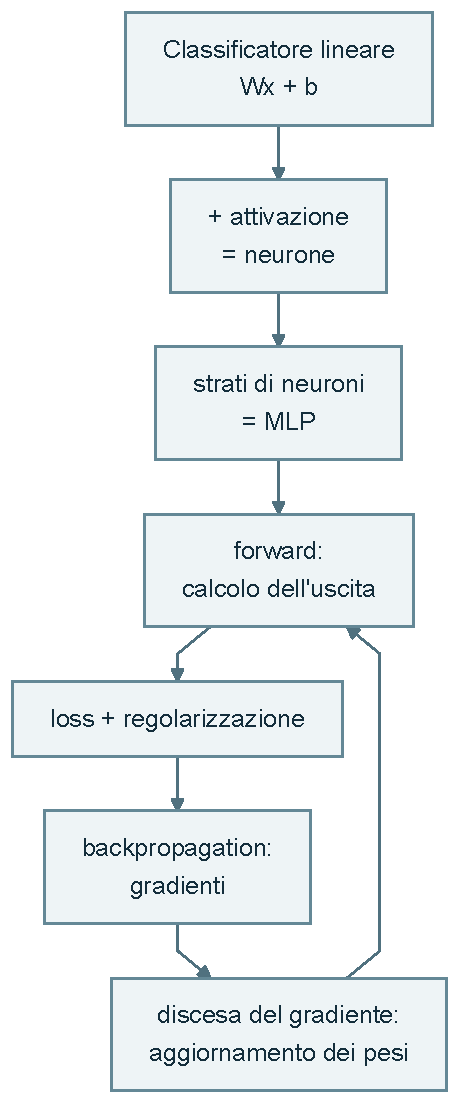
\includegraphics[keepaspectratio]{figure/diagramma_f01_01.pdf}}
% END F01-B0003

% BEGIN F01-B0004
\begin{center}\rule{0.5\linewidth}{0.5pt}\end{center}
% END F01-B0004

% BEGIN F01-B0005
\section{Introduzione}\label{f01-r31}
% END F01-B0005

% BEGIN F01-B0006
\subsection{Perché studiare il Deep Learning (slide 4)}\label{f01-r33}
% END F01-B0006

% BEGIN F01-B0007
Gran parte dei risultati dell\textquotesingle IA moderna si fonda su sistemi di deep learning:
% END F01-B0007

% BEGIN F01-B0008
\begin{itemize}
\tightlist
\item
  IA generativa e \emph{large language models};
\item
  IA per la chimica (progettazione di proteine e farmaci);
\item
  la parte di \textbf{percezione} della guida autonoma;
\item
  in robotica, i modelli \textbf{Vision-Language-Action (VLA)}, che uniscono interpretazione del linguaggio, percezione e decisione per muovere il robot.
\end{itemize}
% END F01-B0008

% BEGIN F01-B0009
Questi sistemi sono in larga parte \textbf{indipendenti dall\textquotesingle applicazione}. Come in tutto il machine learning, una volta che si sa come sono fatti i modelli, come combinarli e come addestrarli, l\textquotesingle applicazione diventa secondaria: si prendono i dati del dominio e, se il modello è ben progettato, funziona.
% END F01-B0009

% BEGIN F01-B0010
Molte "novità" sono in realtà un \textbf{rebranding} di tecniche di 10--15 anni fa: i \emph{world models} sono in sostanza autoencoder (li vedremo nel corso) e gli LLM come GPT sono il \emph{decoder} del Transformer. Quello che va padroneggiato è il machine learning che sta sotto, non l\textquotesingle etichetta applicativa.
% END F01-B0010

% BEGIN F01-B0011
\begin{figure}[H]
\centering
\pandocbounded{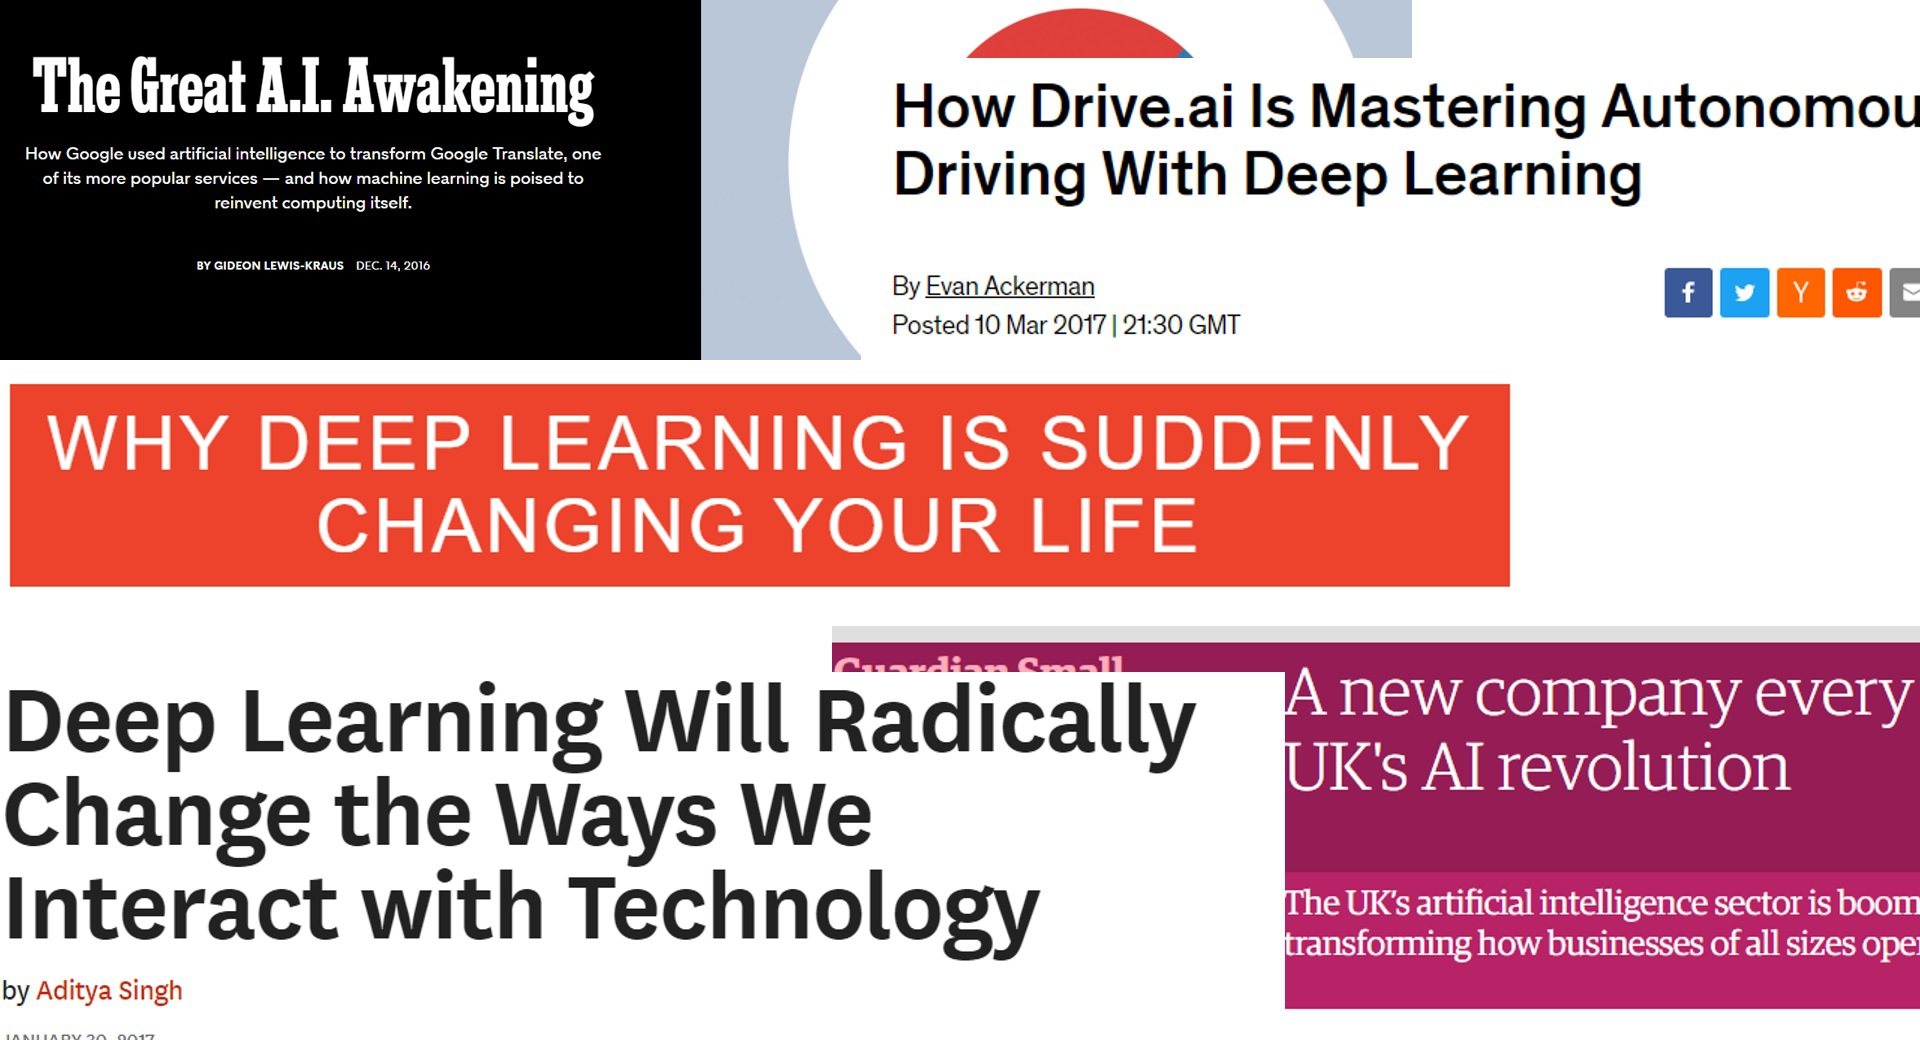
\includegraphics[keepaspectratio]{figure/fig_587f2edfed724a8d.jpg}}
\caption{Slide 4 -- Here is the HYPE}
\end{figure}
% END F01-B0011

% BEGIN F01-B0012
\subsection{Le reti neurali non sono nuove: tre ondate (slide 5)}\label{f01-r48}
% END F01-B0012

% BEGIN F01-B0013
\begin{longtable}[]{@{}
  >{\raggedright\arraybackslash}p{(\linewidth - 2\tabcolsep) * \real{0.5000}}
  >{\raggedright\arraybackslash}p{(\linewidth - 2\tabcolsep) * \real{0.5000}}@{}}
\toprule\noalign{}
\begin{minipage}[b]{\linewidth}\raggedright
Periodo
\end{minipage} & \begin{minipage}[b]{\linewidth}\raggedright
Cosa succede
\end{minipage} \\
\midrule\noalign{}
\endhead
\bottomrule\noalign{}
\endlastfoot
\textbf{1940--1960} & Teorie di apprendimento ispirate alla biologia; primi modelli pionieristici come il \textbf{perceptron}. Per la prima volta si addestra un singolo neurone. \\
\textbf{1980--1990} & Reti con un paio di strati nascosti addestrate con \textbf{backpropagation} (1986). \\
\textbf{2006--oggi} & Ondata attuale di ricerca. \\
\end{longtable}
% END F01-B0013

% BEGIN F01-B0014
Negli anni \textquotesingle80 le reti si scontrarono con due limiti: \textbf{mancava la potenza di calcolo} e \textbf{mancavano i dati}, e le reti neurali sono modelli molto \emph{data hungry}.
% END F01-B0014

% BEGIN F01-B0015
\subsection{Perché proprio ora? (slide 6--9)}\label{f01-r58}
% END F01-B0015

% BEGIN F01-B0016
Le idee di base esistevano da tempo, ma le prestazioni sono esplose solo di recente grazie a fattori complementari:
% END F01-B0016

% BEGIN F01-B0017
\begin{itemize}
\tightlist
\item
  grandi dataset etichettati;
\item
  potenza di calcolo;
\item
  addestramento su \textbf{GPU} (eventualmente distribuito).
\end{itemize}
% END F01-B0017

% BEGIN F01-B0018
La crescita della scala dei dati è stata più che lineare, quasi esponenziale:
% END F01-B0018

% BEGIN F01-B0019
\begin{itemize}
\tightlist
\item
  \textbf{2003} (Fergus, Perona, Zisserman): un dataset "grande" contava \textbf{fino a 400 immagini} (slide 7);
\item
  \textbf{2017} (YouTube-BoundingBoxes, Real et al.): \textbf{240.000 video}, 5,6 milioni di bounding box e 10,5 milioni di annotazioni umane (slide 8).
\end{itemize}
% END F01-B0019

% BEGIN F01-B0020
\begin{figure}[H]
\centering
\pandocbounded{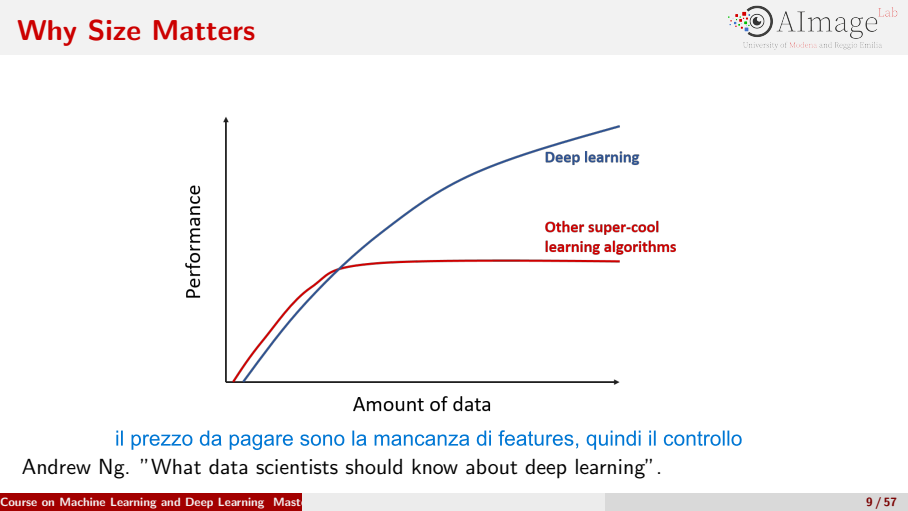
\includegraphics[keepaspectratio]{figure/fig_2c71462bd05909de.png}}
\caption{Slide 9 -- Why Size Matters (Andrew Ng)}
\end{figure}
% END F01-B0020

% BEGIN F01-B0021
Il grafico di Andrew Ng (slide 9) riassume il punto:
% END F01-B0021

% BEGIN F01-B0022
\begin{itemize}
\tightlist
\item
  con pochi dati, gli algoritmi classici e il deep learning si equivalgono;
\item
  aumentando i dati, gli algoritmi classici raggiungono un \textbf{plateau}, mentre il deep learning \textbf{continua a migliorare}.
\end{itemize}
% END F01-B0022

% BEGIN F01-B0023
Per questo la "magia" di sistemi come GPT non è stata tecnica: si è presa un\textquotesingle architettura già esistente (il Transformer, 2017) e la si è riempita con un\textquotesingle enorme quantità di dati.
% END F01-B0023

% BEGIN F01-B0024
\subsection{Il problema della rappresentazione dei dati (slide 10)}\label{f01-r80}
% END F01-B0024

% BEGIN F01-B0025
Le prestazioni di un algoritmo di ML dipendono fortemente da \textbf{come rappresentiamo i dati}. Le \textbf{feature} sono i pezzi discreti d\textquotesingle informazione che usiamo come \emph{proxy} per modellare la complessità del mondo. Per molto tempo sono state \textbf{progettate a mano} (\emph{handcrafted}), in modo diverso per ogni compito. Il deep learning invece \textbf{impara la rappresentazione direttamente dai dati}.
% END F01-B0025

% BEGIN F01-B0026
\pandocbounded{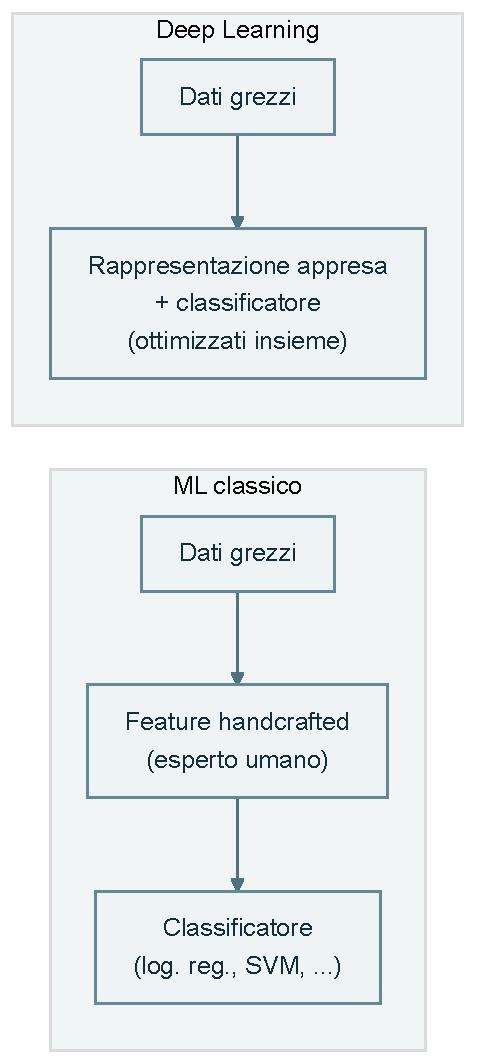
\includegraphics[keepaspectratio]{figure/diagramma_f01_02.pdf}}
% END F01-B0026

% BEGIN F01-B0027
\textbf{Perché le feature fissate impongono un tetto.} Supponiamo di classificare immagini usando come unica feature il \textbf{colore medio}. Non si raggiungerà mai il 100\% di accuratezza, qualunque classificatore e qualunque quantità di dati si usi: la feature è troppo povera. Fissare le feature significa fissare implicitamente anche un \textbf{tetto alle prestazioni} (\emph{performance cap}): le feature sono il "carburante" del sistema di ML.
% END F01-B0027

% BEGIN F01-B0028
\textbf{Cosa cambia con il deep learning.} Una rete neurale risolve \textbf{contemporaneamente due problemi}:
% END F01-B0028

% BEGIN F01-B0029
\begin{enumerate}
\def\labelenumi{\arabic{enumi}.}
\tightlist
\item
  partendo dal dato il più grezzo possibile, \textbf{estrae una rappresentazione} adatta al problema;
\item
  su questa rappresentazione, \textbf{costruisce il classificatore}.
\end{enumerate}
% END F01-B0029

% BEGIN F01-B0030
I due problemi sono accoppiati: la rappresentazione appresa è quella più utile per minimizzare la loss. Se le feature possono cambiare, all\textquotesingle aumentare dei dati la rete impara feature sempre più espressive e può migliorare le prestazioni, senza garantirne la convergenza al 100\%. È questa la spiegazione della curva blu della slide 9.
% END F01-B0030

% BEGIN F01-B0031
\begin{quote}
\textbf{Il prezzo da pagare: la perdita di controllo}
\end{quote}
% END F01-B0031

% BEGIN F01-B0032
\begin{quote}
La rete rappresenta il mondo con feature scelte \textbf{per risolvere la loss}, non secondo le nostre categorie. Per queste feature \textbf{non abbiamo un nome}, e ciò che non si può nominare non si può davvero capire. Si possono estrarre dal modello spiegazioni o regole, ma il "carburante" resta privo di significato per un essere umano. L\textquotesingle idea che si possano comprendere fino in fondo le rappresentazioni interne di un modello profondo è quindi falsa. (Annotazione slide 9: \emph{"il prezzo da pagare è la mancanza di feature {[}interpretabili{]}, quindi il controllo"}.)
\end{quote}
% END F01-B0032

% BEGIN F01-B0033
\begin{center}\rule{0.5\linewidth}{0.5pt}\end{center}
% END F01-B0033

% BEGIN F01-B0034
\section{Un passo indietro: i classificatori lineari}\label{f01-r108}
% END F01-B0034

% BEGIN F01-B0035
Un \textbf{classificatore lineare} è un classificatore in cui la mappa è affine nell'input a parametri fissati e affine nei parametri a input fissato, ma non congiuntamente lineare nelle due variabili: calcola una \textbf{somma pesata} degli input. In 2D separa gli oggetti con una retta; in più dimensioni con un piano o un iperpiano. Conviene ripartire da qui perché \textbf{una rete neurale è una collezione di classificatori lineari}, ed è sorprendente che basti combinarli per ottenere modelli così potenti.
% END F01-B0035

% BEGIN F01-B0036
\subsection{Formalizzazione (slide 12--14)}\label{f01-r112}
% END F01-B0036

% BEGIN F01-B0037
Ci concentriamo sulla \textbf{classificazione di immagini}. Il training set contiene \(N\) immagini:
% END F01-B0037

% BEGIN F01-B0038
\begin{center}
\begin{adjustbox}{max width=\linewidth}
$\displaystyle 
x_i \in \mathbb{R}^D,\quad i = 1,\dots,N, \qquad (x_i, y_i),\; y_i \in \{1,\dots,K\}
$
\end{adjustbox}
\end{center}
% END F01-B0038

% BEGIN F01-B0039
L\textquotesingle obiettivo è una funzione \(f:\mathbb{R}^D \to \mathbb{R}^K\) che associa a ogni immagine \textbf{un punteggio (score) per ciascuna classe}; la classe predetta è quella con lo score più alto. La mappa lineare è:
% END F01-B0039

% BEGIN F01-B0040
\begin{center}
\begin{adjustbox}{max width=\linewidth}
$\displaystyle 
\boxed{f(x_i, W, b) = W x_i + b}
$
\end{adjustbox}
\end{center}
% END F01-B0040

% BEGIN F01-B0041
\textbf{Esempio CIFAR-10 (slide 13--14).} Il dataset contiene \(N = 60\,000\) immagini RGB \(32\times32\) divise in \(K = 10\) classi.
% END F01-B0041

% BEGIN F01-B0042
\begin{figure}[H]
\centering
\pandocbounded{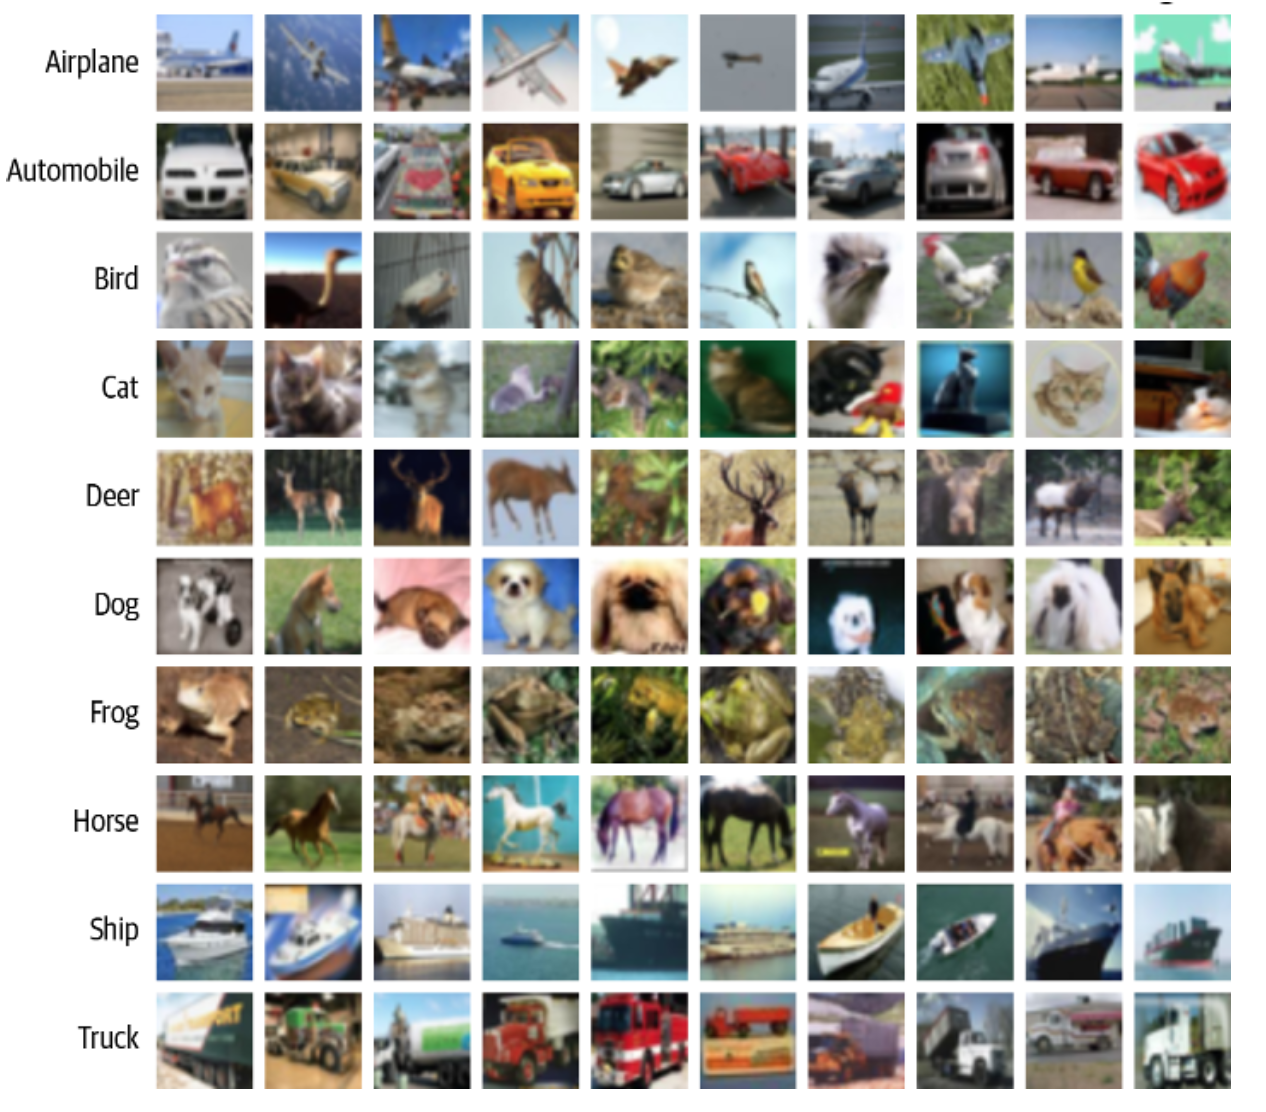
\includegraphics[keepaspectratio]{figure/fig_26a247fabde99104.png}}
\caption{Slide 13 -- CIFAR-10}
\end{figure}
% END F01-B0042

% BEGIN F01-B0043
Ogni immagine ha 3 canali (R, G, B) e va "srotolata" in un vettore colonna:
% END F01-B0043

% BEGIN F01-B0044
\begin{center}
\begin{adjustbox}{max width=\linewidth}
$\displaystyle 
D = 32 \times 32 \times 3 = 3072 \;\Rightarrow\; x_i \in \mathbb{R}^{3072}
$
\end{adjustbox}
\end{center}
% END F01-B0044

% BEGIN F01-B0045
\begin{itemize}
\tightlist
\item
  \(W \in \mathbb{R}^{10\times3072}\) è la \textbf{matrice dei pesi}: una riga per classe, cioè 10 righe da 3072 coefficienti. Ogni riga contiene i parametri che producono lo score di una classe.
\item
  \(b \in \mathbb{R}^{10}\) è il \textbf{vettore dei bias}.
\item
  \(Wx_i + b \in \mathbb{R}^{10}\) contiene i 10 score.
\end{itemize}
% END F01-B0045

% BEGIN F01-B0046
Si vuole imparare \(W, b\) dal training set in modo che, per una nuova immagine \(x^{test}\), \textbf{lo score della classe corretta sia più alto degli score delle altre classi}.
% END F01-B0046

% BEGIN F01-B0047
\textbf{Il bias.} Se i dati non sono centrati nell\textquotesingle origine, il bias permette di \textbf{traslare} l\textquotesingle iperpiano di separazione. È importante, ma non cambia la sostanza matematica: si può sempre \textbf{assorbire nei dati}. Basta aggiungere a \(x\) una componente costante pari a 1 e a \(W\) una colonna con i bias:
% END F01-B0047

% BEGIN F01-B0048
\begin{center}
\begin{adjustbox}{max width=\linewidth}
$\displaystyle 
Wx + b = \begin{bmatrix} W & b \end{bmatrix}\begin{bmatrix} x \\ 1 \end{bmatrix} = W'x'
$
\end{adjustbox}
\end{center}
% END F01-B0048

% BEGIN F01-B0049
\subsection{Esempio numerico (slide 15)}\label{f01-r148}
% END F01-B0049

% BEGIN F01-B0050
È la stessa formula \(f(x) = Wx + b\) del caso CIFAR-10, ma in miniatura, così i conti si fanno a mano: un\textquotesingle immagine di \textbf{4 pixel in scala di grigi} (\(D = 4\)) e \textbf{3 classi}, gatto, cane e nave (\(K = 3\)).
% END F01-B0050

% BEGIN F01-B0051
\begin{figure}[H]
\centering
\pandocbounded{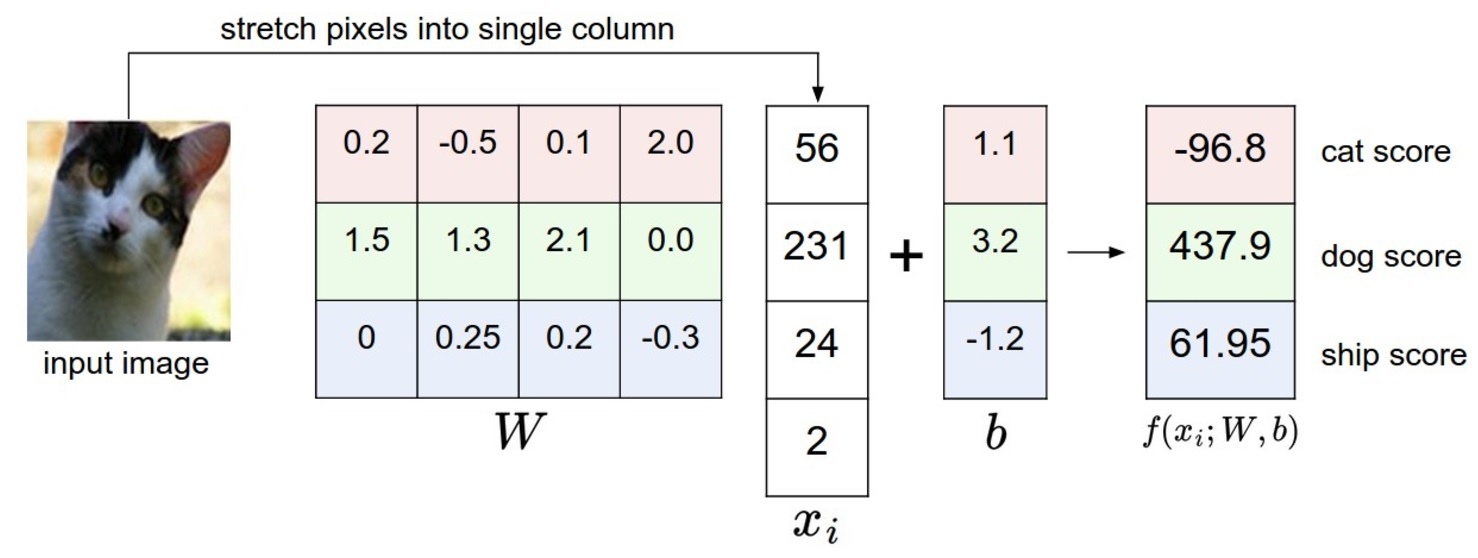
\includegraphics[keepaspectratio]{figure/fig_c2fb496bd32f35f0.jpg}}
\caption{Slide 15 -- Mappare un\textquotesingle immagine sugli score}
\end{figure}
% END F01-B0051

% BEGIN F01-B0052
\textbf{Passo 1: l\textquotesingle immagine diventa un vettore.} L\textquotesingle immagine è \(2\times2\) e ogni pixel è un\textquotesingle intensità di grigio tra 0 (nero) e 255 (bianco). La si "stira" in una colonna (\emph{stretch pixels into single column}):
% END F01-B0052

% BEGIN F01-B0053
\begin{center}
\begin{adjustbox}{max width=\linewidth}
$\displaystyle 
\begin{bmatrix}56 & 231\\ 24 & 2\end{bmatrix} \;\longrightarrow\; x = \begin{bmatrix}56\\231\\24\\2\end{bmatrix} \in \mathbb{R}^4
$
\end{adjustbox}
\end{center}
% END F01-B0053

% BEGIN F01-B0054
\textbf{Passo 2: i parametri.} \(W\) ha \textbf{una riga per classe} e \textbf{una colonna per pixel}, quindi è \(3\times4\). La riga \(k\) dice quanto conta ciascun pixel per la classe \(k\):
% END F01-B0054

% BEGIN F01-B0055
\begin{itemize}
\tightlist
\item
  un peso positivo significa "se questo pixel è chiaro, lo score della classe sale";
\item
  un peso negativo significa il contrario.
\end{itemize}
% END F01-B0055

% BEGIN F01-B0056
Il bias \(b\) aggiunge un valore fisso per ogni classe.
% END F01-B0056

% BEGIN F01-B0057
\begin{center}
\begin{adjustbox}{max width=\linewidth}
$\displaystyle 
W = \begin{bmatrix} 0.2 & -0.5 & 0.1 & 2.0 \\ 1.5 & 1.3 & 2.1 & 0.0 \\ 0 & 0.25 & 0.2 & -0.3 \end{bmatrix}\begin{matrix}\leftarrow \text{gatto}\\ \leftarrow \text{cane}\\ \leftarrow \text{nave}\end{matrix}
\qquad
b = \begin{bmatrix}1.1\\3.2\\-1.2\end{bmatrix}
$
\end{adjustbox}
\end{center}
% END F01-B0057

% BEGIN F01-B0058
\textbf{Passo 3: uno score per classe.} Ogni score è il \textbf{prodotto scalare} tra la riga della classe e \(x\) (pixel per peso, poi somma), più il bias della classe:
% END F01-B0058

% BEGIN F01-B0059
\begin{center}
\begin{adjustbox}{max width=\linewidth}
$\displaystyle 
s_k = \sum_{j=1}^{4} W_{kj}\,x_j + b_k
$
\end{adjustbox}
\end{center}
% END F01-B0059

% BEGIN F01-B0060
\begin{longtable}[]{@{}
  >{\raggedright\arraybackslash}p{(\linewidth - 14\tabcolsep) * \real{0.1250}}
  >{\raggedright\arraybackslash}p{(\linewidth - 14\tabcolsep) * \real{0.1250}}
  >{\raggedright\arraybackslash}p{(\linewidth - 14\tabcolsep) * \real{0.1250}}
  >{\raggedright\arraybackslash}p{(\linewidth - 14\tabcolsep) * \real{0.1250}}
  >{\raggedright\arraybackslash}p{(\linewidth - 14\tabcolsep) * \real{0.1250}}
  >{\raggedright\arraybackslash}p{(\linewidth - 14\tabcolsep) * \real{0.1250}}
  >{\raggedright\arraybackslash}p{(\linewidth - 14\tabcolsep) * \real{0.1250}}
  >{\raggedright\arraybackslash}p{(\linewidth - 14\tabcolsep) * \real{0.1250}}@{}}
\toprule\noalign{}
\begin{minipage}[b]{\linewidth}\raggedright
Classe
\end{minipage} & \begin{minipage}[b]{\linewidth}\raggedright
pixel 1 (56)
\end{minipage} & \begin{minipage}[b]{\linewidth}\raggedright
pixel 2 (231)
\end{minipage} & \begin{minipage}[b]{\linewidth}\raggedright
pixel 3 (24)
\end{minipage} & \begin{minipage}[b]{\linewidth}\raggedright
pixel 4 (2)
\end{minipage} & \begin{minipage}[b]{\linewidth}\raggedright
somma
\end{minipage} & \begin{minipage}[b]{\linewidth}\raggedright
+ bias
\end{minipage} & \begin{minipage}[b]{\linewidth}\raggedright
\textbf{score}
\end{minipage} \\
\midrule\noalign{}
\endhead
\bottomrule\noalign{}
\endlastfoot
gatto & \(0.2\cdot56 = 11.2\) & \(-0.5\cdot231 = -115.5\) & \(0.1\cdot24 = 2.4\) & \(2.0\cdot2 = 4.0\) & \(-97.9\) & \(+1.1\) & \textbf{−96.8} \\
cane & \(1.5\cdot56 = 84.0\) & \(1.3\cdot231 = 300.3\) & \(2.1\cdot24 = 50.4\) & \(0.0\cdot2 = 0\) & \(434.7\) & \(+3.2\) & \textbf{437.9} \\
nave & \(0\cdot56 = 0\) & \(0.25\cdot231 = 57.75\) & \(0.2\cdot24 = 4.8\) & \(-0.3\cdot2 = -0.6\) & \(61.95\) & \(-1.2\) & \textbf{60.75} \\
\end{longtable}
% END F01-B0060

% BEGIN F01-B0061
In forma matriciale sono le tre righe dello stesso prodotto: \(Wx + b = [-96.8,\ 437.9,\ 60.75]^T\).
% END F01-B0061

% BEGIN F01-B0062
\textbf{Passo 4: la predizione.} Vince la classe con lo score più alto, cioè \textbf{cane}. L\textquotesingle immagine però è un gatto: la predizione è \textbf{sbagliata}, perché i pesi sono arbitrari e non addestrati. Addestrare il classificatore significa proprio \textbf{modificare \(W\) e \(b\)} finché, per le immagini di gatto, è la riga "gatto" a dare lo score più alto.
% END F01-B0062

% BEGIN F01-B0063
Il pixel 2 (231) è molto chiaro: la riga "cane" gli assegna un peso positivo alto (1.3), la riga "gatto" un peso negativo (−0.5). Da solo, questo pixel sposta gli score di centinaia di punti.
% END F01-B0063

% BEGIN F01-B0064
\begin{quote}
\textbf{Errata slide 15}
\end{quote}
% END F01-B0064

% BEGIN F01-B0065
\begin{quote}
La slide riporta \(s_{ship} = 61.95\), che è il valore di \(w_3^T x\) \textbf{senza} il bias \(-1.2\). Il valore corretto è \textbf{60.75}. Gli altri due score sono corretti.
\end{quote}
% END F01-B0065

% BEGIN F01-B0066
\textbf{Cosa c\textquotesingle è di sbagliato in questi score?} \textbf{Non sono normalizzati.} \(437.9\) è un valore alto o basso? Non si può dire: gli score vivono in \((-\infty, +\infty)\), non sommano a 1 e non hanno una scala di riferimento. Serve una funzione che li trasformi in quantità confrontabili, come nella regressione logistica.
% END F01-B0066

% BEGIN F01-B0067
\subsection{Regressione logistica e binary cross-entropy (slide 16--17)}\label{f01-r196}
% END F01-B0067

% BEGIN F01-B0068
Aggiungendo una non linearità sigmoide alla mappa lineare si ottiene la \textbf{regressione logistica}:
% END F01-B0068

% BEGIN F01-B0069
\begin{center}
\begin{adjustbox}{max width=\linewidth}
$\displaystyle 
f(x_i, W, b) = \sigma(Wx_i + b), \qquad \sigma(x) = \frac{1}{1+e^{-x}}
$
\end{adjustbox}
\end{center}
% END F01-B0069

% BEGIN F01-B0070
La si addestra minimizzando la \textbf{binary cross-entropy} su \(m\) esempi, dove \(f_{x_i}\) indica \(f(x_i,W,b)\):
% END F01-B0070

% BEGIN F01-B0071
\begin{center}
\begin{adjustbox}{max width=\linewidth}
$\displaystyle 
\boxed{\mathcal{L}(W,b) = -\frac{1}{m}\sum_{i=1}^{m}\Big( y_i \log f_{x_i} + (1-y_i)\log(1-f_{x_i}) \Big), \qquad y_i\in\{0,1\}}
$
\end{adjustbox}
\end{center}
% END F01-B0071

% BEGIN F01-B0072
\begin{figure}[H]
\centering
\pandocbounded{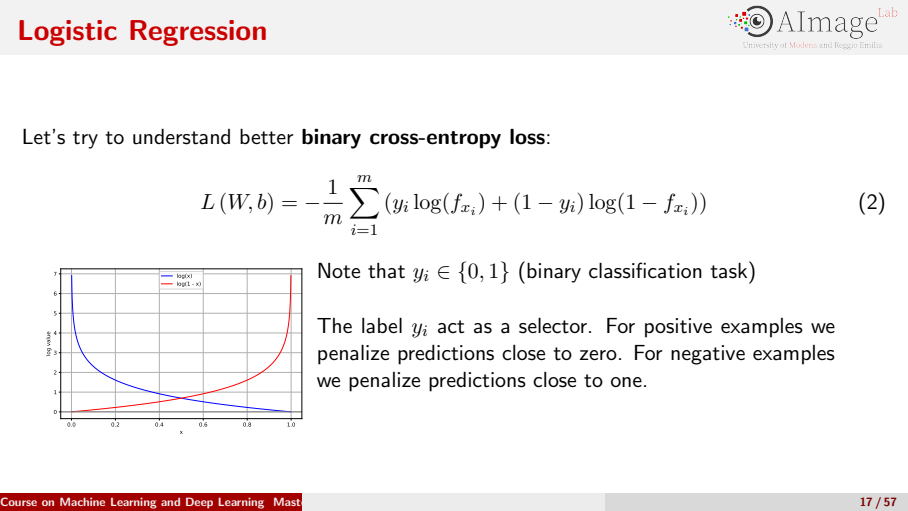
\includegraphics[keepaspectratio]{figure/fig_0b683e968aa69224.png}}
\caption{Slide 17 -- Le due componenti della BCE}
\end{figure}
% END F01-B0072

% BEGIN F01-B0073
L\textquotesingle etichetta \(y_i\) fa da \textbf{selettore}:
% END F01-B0073

% BEGIN F01-B0074
\begin{itemize}
\tightlist
\item
  se \(y_i = 1\), il secondo termine si annulla (\(1-y_i = 0\)) e resta \(-\log f_{x_i}\). Vale 0 se \(f_{x_i} = 1\) e tende a \(+\infty\) se \(f_{x_i}\to 0\): \textbf{penalizza le predizioni vicine a 0};
\item
  se \(y_i = 0\), il primo termine si annulla e resta \(-\log(1-f_{x_i})\), che \textbf{penalizza le predizioni vicine a 1}.
\end{itemize}
% END F01-B0074

% BEGIN F01-B0075
In pratica si prende lo score che il modello assegna alla classe giusta e lo si vuole \textbf{alzare}, cioè si vuole abbassare il suo \(-\log\).
% END F01-B0075

% BEGIN F01-B0076
\subsection{Classificatore Softmax (slide 18--19)}\label{f01-r219}
% END F01-B0076

% BEGIN F01-B0077
Il \textbf{classificatore Softmax} generalizza la regressione logistica al caso multiclasse. La funzione softmax prende un vettore \(z\) di score reali arbitrari e lo "schiaccia" in valori tra 0 e 1 che sommano a 1:
% END F01-B0077

% BEGIN F01-B0078
\begin{center}
\begin{adjustbox}{max width=\linewidth}
$\displaystyle 
\boxed{\text{softmax}_j(z) = \frac{e^{z_j}}{\sum_{k=1}^{K} e^{z_k}}}
$
\end{adjustbox}
\end{center}
% END F01-B0078

% BEGIN F01-B0079
\textbf{Calcolo passo passo dell\textquotesingle esempio della slide 18}, con \(z = [1.2,\ 5.1,\ 2.7]\):
% END F01-B0079

% BEGIN F01-B0080
\begin{longtable}[]{@{}llll@{}}
\toprule\noalign{}
& \(z_j\) & \(e^{z_j}\) & \(e^{z_j} / \sum_k e^{z_k}\) \\
\midrule\noalign{}
\endhead
\bottomrule\noalign{}
\endlastfoot
classe 1 & 1.2 & 3.32 & \textbf{0.018} \\
classe 2 & 5.1 & 164.02 & \textbf{0.900} \\
classe 3 & 2.7 & 14.88 & \textbf{0.082} \\
somma & & 182.22 & 1 \\
\end{longtable}
% END F01-B0080

% BEGIN F01-B0081
Rispetto alla regressione logistica multiclasse vista nel corso precedente, che modellava \(K-1\) classi e ricavava la \(K\)-esima per complemento, qui si tratta \textbf{allo stesso modo tutte le \(K\) classi}: esponenziale di ogni score, diviso la somma di tutti gli esponenziali. Si usa un insieme di parametri in più, ma la formulazione è più semplice.
% END F01-B0081

% BEGIN F01-B0082
\textbf{La softmax produce una distribuzione di probabilità del modello:} ogni componente è positiva e la somma è 1. Questo non garantisce che i valori coincidano con le frequenze reali delle classi. Non è una soglia rigida e non spinge necessariamente il massimo vicino a 1: score tutti uguali producono \(1/K\) per classe. Le differenze fra score, non i loro rapporti, determinano i rapporti tra probabilità.
% END F01-B0082

% BEGIN F01-B0083
Il motivo sta nell\textquotesingle esponenziale: il rapporto tra due uscite dipende dalla \textbf{differenza} degli score, non dal loro rapporto:
% END F01-B0083

% BEGIN F01-B0084
\begin{center}
\begin{adjustbox}{max width=\linewidth}
$\displaystyle 
\frac{\text{softmax}_2}{\text{softmax}_3} = \frac{e^{5.1}}{e^{2.7}} = e^{5.1-2.7} = e^{2.4} \approx 11
$
\end{adjustbox}
\end{center}
% END F01-B0084

% BEGIN F01-B0085
L\textquotesingle annotazione «stiamo semplicemente applicando una soglia» va intesa come analogia con una decisione morbida. La decisione discreta avviene dopo, scegliendo \(\arg\max_j p_j\) (oppure confrontando una probabilità binaria con una soglia). La calibrazione riguarda l\textquotesingle attendibilità delle probabilità, non la loro validità matematica.
% END F01-B0085

% BEGIN F01-B0086
Nel classificatore softmax gli score \(f(x_i,W) = Wx_i\) sono interpretati come \textbf{log-probabilità non normalizzate}, e lo si addestra con la \textbf{cross-entropy}:
% END F01-B0086

% BEGIN F01-B0087
\begin{center}
\begin{adjustbox}{max width=\linewidth}
$\displaystyle 
\mathcal{L} = -\sum_{k} y^{true}_{k}\,\log\big(y^{pred}_{k}\big)
$
\end{adjustbox}
\end{center}
% END F01-B0087

% BEGIN F01-B0088
dove \(y^{true}\) è la distribuzione vera (un vettore \textbf{one-hot} che seleziona la classe corretta) e \(y^{pred} = \text{softmax}(f)\). La forma esplicita per il singolo esempio è derivata in §7.2.
% END F01-B0088

% BEGIN F01-B0089
\begin{quote}
\textbf{Errata slide 18--19}
\end{quote}
% END F01-B0089

% BEGIN F01-B0090
\begin{quote}
Nella slide 18 il denominatore è scritto \(\sum_k e^{z_j}\): l\textquotesingle indice corretto è \(\sum_k e^{z_k}\). Nella slide 19 manca il segno \textbf{meno} davanti alla cross-entropy.
\end{quote}
% END F01-B0090

% BEGIN F01-B0091
\textbf{Riepilogo:}
% END F01-B0091

% BEGIN F01-B0092
\begin{center}
\begin{adjustbox}{max width=\linewidth}
$\displaystyle 
\underbrace{Wx+b}_{\text{classificatore lineare}} \;+\; \text{softmax} \;+\; \text{cross-entropy} \;+\; \text{discesa del gradiente} \;=\; \textbf{regressione logistica}
$
\end{adjustbox}
\end{center}
% END F01-B0092

% BEGIN F01-B0093
\begin{center}\rule{0.5\linewidth}{0.5pt}\end{center}
% END F01-B0093

% BEGIN F01-B0094
\section{Modellare un neurone}\label{f01-r267}
% END F01-B0094

% BEGIN F01-B0095
\subsection{Il neurone biologico (slide 21)}\label{f01-r269}
% END F01-B0095

% BEGIN F01-B0096
Le reti neurali sono un modello matematico \textbf{ispirato in modo grossolano} (\emph{coarsely}) al funzionamento del cervello. Il neurone ne è l\textquotesingle unità computazionale di base: ne abbiamo circa \textbf{86 miliardi}, collegati da circa \(10^{14}\)--\(10^{15}\) \textbf{sinapsi}. Ogni neurone riceve segnali dai \textbf{dendriti} e produce l\textquotesingle uscita lungo il suo (unico) \textbf{assone}, che si ramifica e si collega tramite sinapsi ai dendriti di altri neuroni.
% END F01-B0096

% BEGIN F01-B0097
\begin{figure}[H]
\centering
\pandocbounded{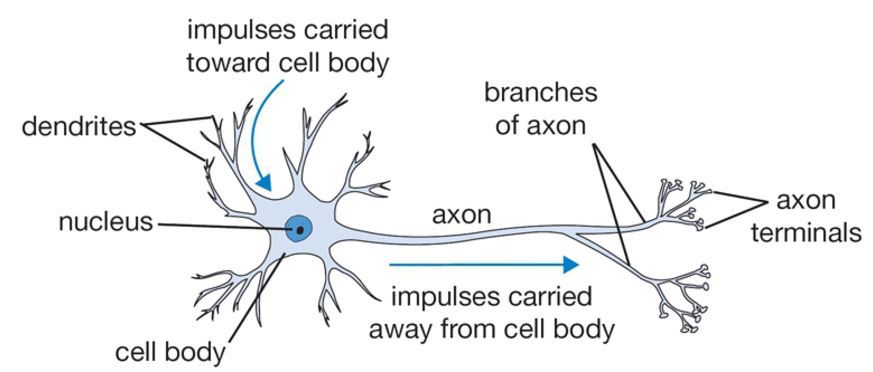
\includegraphics[keepaspectratio]{figure/fig_fad5c4c0b45f5c29.jpg}}
\caption{Slide 21 -- Neurone biologico}
\end{figure}
% END F01-B0097

% BEGIN F01-B0098
L\textquotesingle analogia utile associa la forza delle connessioni ai pesi, la combinazione dei segnali alla somma pesata e la risposta del neurone all\textquotesingle attivazione. Non è una descrizione fisiologica letterale: in particolare l\textquotesingle immagine di una sinapsi «dura o morbida» è soltanto una metafora della modulazione del segnale. Il neurone biologico ha una dinamica temporale che questa mappa statica non rappresenta.
% END F01-B0098

% BEGIN F01-B0099
\subsection{Il neurone artificiale (slide 22--23)}\label{f01-r277}
% END F01-B0099

% BEGIN F01-B0100
La traduzione in matematica è uno a uno:
% END F01-B0100

% BEGIN F01-B0101
\begin{longtable}[]{@{}
  >{\raggedright\arraybackslash}p{(\linewidth - 2\tabcolsep) * \real{0.5000}}
  >{\raggedright\arraybackslash}p{(\linewidth - 2\tabcolsep) * \real{0.5000}}@{}}
\toprule\noalign{}
\begin{minipage}[b]{\linewidth}\raggedright
Biologia
\end{minipage} & \begin{minipage}[b]{\linewidth}\raggedright
Matematica
\end{minipage} \\
\midrule\noalign{}
\endhead
\bottomrule\noalign{}
\endlastfoot
Dendriti (ingressi) & input \(x_i\) \\
Sinapsi (amplifica/attenua) & moltiplicazione per un peso \(w_i\) (grande o piccolo) \\
Cellula (mette insieme i segnali) & \textbf{somma}: \(\sum_i w_i x_i + b\) \\
Soglia di accensione & \textbf{funzione di attivazione} \(f(\cdot)\) \\
Assone (uscita) & \(y = f\big(\sum_i w_i x_i + b\big)\) \\
\end{longtable}
% END F01-B0101

% BEGIN F01-B0102
\begin{figure}[H]
\centering
\pandocbounded{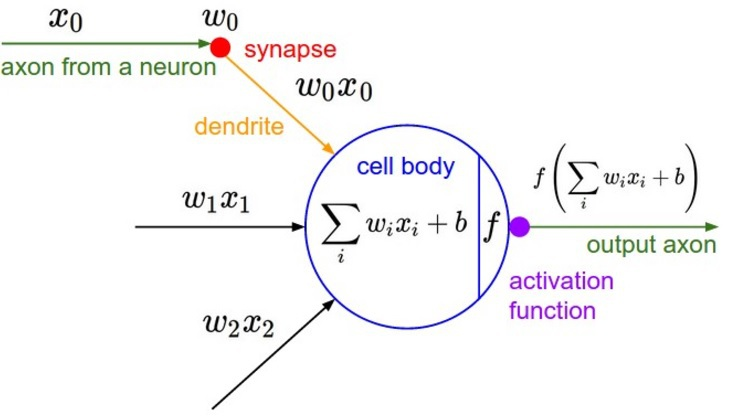
\includegraphics[keepaspectratio]{figure/fig_329091fd2ed8702d.jpg}}
\caption{Slide 22 -- Modello del singolo neurone}
\end{figure}
% END F01-B0102

% BEGIN F01-B0103
Un neurone può avere più ingressi. La sua uscita è il \textbf{prodotto scalare tra ingressi e pesi, più il bias, a cui si applica una non linearità}:
% END F01-B0103

% BEGIN F01-B0104
\begin{center}
\begin{adjustbox}{max width=\linewidth}
$\displaystyle 
\boxed{y = f\!\left(w^T x + b\right)}
$
\end{adjustbox}
\end{center}
% END F01-B0104

% BEGIN F01-B0105
È il \textbf{perceptron} di McCulloch e Pitts (anni \textquotesingle40).
% END F01-B0105

% BEGIN F01-B0106
\begin{quote}
\textbf{Neurone = regressione logistica (slide 23)}
\end{quote}
% END F01-B0106

% BEGIN F01-B0107
\begin{quote}
Una combinazione affine seguita dalla \textbf{sigmoide} definisce il modello di regressione logistica binaria. Se il neurone usa la sigmoide ed è addestrato con la binary cross-entropy tramite discesa del gradiente, gli ingredienti sono gli stessi, al 100\%: stesse equazioni, quindi stesso modello.

\textbf{Il grado di libertà in più:} nulla impone che la funzione di sogliatura sia la sigmoide o la softmax, se ne può usare qualunque. Prende il nome di \textbf{funzione di attivazione} perché stabilisce se il neurone è attivo (acceso) oppure no.
\end{quote}
% END F01-B0107

% BEGIN F01-B0108
\subsection{Funzioni di attivazione (slide 24--26)}\label{f01-r304}
% END F01-B0108

% BEGIN F01-B0109
Le funzioni di attivazione sono \textbf{funzioni non lineari} calcolate sull\textquotesingle uscita di ogni neurone. Le più usate storicamente sono \textbf{sigmoide, tanh e ReLU}; ne esistono anche di più complesse.
% END F01-B0109

% BEGIN F01-B0110
Nel deep learning il successo dipende dai \textbf{dettagli}. Progettare una rete si fa in un pomeriggio, farla addestrare è un\textquotesingle altra storia. Molto spesso il problema non è di progetto ma \textbf{tecnico}:
% END F01-B0110

% BEGIN F01-B0111
\begin{itemize}
\tightlist
\item
  la saturazione del gradiente;
\item
  \textbf{neuroni che non si attivano mai};
\item
  il \textbf{gradiente che svanisce} perché la rete è troppo profonda.
\end{itemize}
% END F01-B0111

% BEGIN F01-B0112
Le attivazioni sono il primo di questi dettagli.
% END F01-B0112

% BEGIN F01-B0113
\subsubsection{Sigmoide}\label{f01-r316}
% END F01-B0113

% BEGIN F01-B0114
\begin{center}
\begin{adjustbox}{max width=\linewidth}
$\displaystyle 
\boxed{\sigma(x) = \frac{1}{1+e^{-x}} = \frac{e^{x}}{1+e^{x}} \in (0,1)}
$
\end{adjustbox}
\end{center}
% END F01-B0114

% BEGIN F01-B0115
La seconda forma si ottiene moltiplicando numeratore e denominatore per \(e^x\) ed è quella della regressione logistica. La curva ha la forma a "S" di una soglia morbida: sopra la soglia spinge verso 1, sotto verso 0.
% END F01-B0115

% BEGIN F01-B0116
\begin{figure}[H]
\centering
\pandocbounded{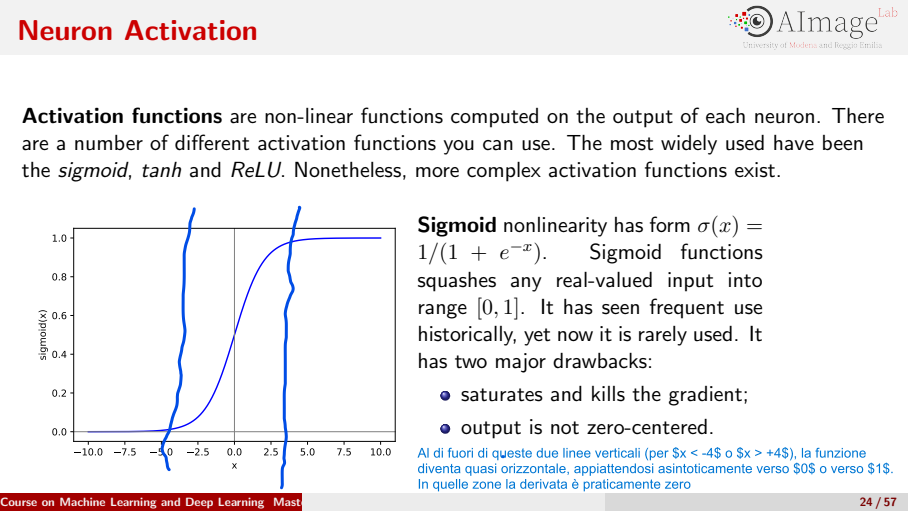
\includegraphics[keepaspectratio]{figure/fig_041dd0c66ee14a3b.png}}
\caption{Slide 24 -- Sigmoide e zone di saturazione}
\end{figure}
% END F01-B0116

% BEGIN F01-B0117
\textbf{La derivata, passo passo.} Serve per capire il secondo difetto della sigmoide.
% END F01-B0117

% BEGIN F01-B0118
\begin{enumerate}
\def\labelenumi{\arabic{enumi}.}
\tightlist
\item
  Si riscrive \(\sigma(x) = (1+e^{-x})^{-1}\).
\item
  Si deriva con la regola della catena, dove la funzione esterna è \(u^{-1}\) e quella interna è \(u = 1+e^{-x}\): \begin{center}
\begin{adjustbox}{max width=\linewidth}
$\displaystyle \sigma'(x) = -(1+e^{-x})^{-2}\cdot\frac{d}{dx}(1+e^{-x}) = -(1+e^{-x})^{-2}\cdot(-e^{-x}) = \frac{e^{-x}}{(1+e^{-x})^2}$
\end{adjustbox}
\end{center}
\item
  Si spezza la frazione in due fattori: \begin{center}
\begin{adjustbox}{max width=\linewidth}
$\displaystyle \sigma'(x) = \frac{1}{1+e^{-x}}\cdot\frac{e^{-x}}{1+e^{-x}}$
\end{adjustbox}
\end{center}
\item
  Si riconosce che il secondo fattore è \(1-\sigma(x)\): \begin{center}
\begin{adjustbox}{max width=\linewidth}
$\displaystyle \frac{e^{-x}}{1+e^{-x}} = \frac{(1+e^{-x})-1}{1+e^{-x}} = 1-\frac{1}{1+e^{-x}} = 1-\sigma(x)$
\end{adjustbox}
\end{center}
\item
  Quindi: \begin{center}
\begin{adjustbox}{max width=\linewidth}
$\displaystyle \boxed{\sigma'(x) = \sigma(x)\big(1-\sigma(x)\big)}$
\end{adjustbox}
\end{center}
\end{enumerate}
% END F01-B0118

% BEGIN F01-B0119
\begin{longtable}[]{@{}lllllll@{}}
\toprule\noalign{}
\(x\) & 0 & 2 & 4 & 5 & 10 & 100 \\
\midrule\noalign{}
\endhead
\bottomrule\noalign{}
\endlastfoot
\(\sigma(x)\) & 0.5 & 0.881 & 0.982 & 0.993 & 0.99995 & ≈ 1 \\
\(\sigma'(x)\) & \textbf{0.25} & 0.105 & 0.018 & 0.0066 & 0.00005 & ≈ 0 \\
\end{longtable}
% END F01-B0119

% BEGIN F01-B0120
Il massimo della derivata è \(0.25\), in \(x = 0\). Già per \(|x| \gtrsim 4\) la derivata è praticamente nulla: sono le zone esterne alle due linee verticali disegnate sulla slide 24.
% END F01-B0120

% BEGIN F01-B0121
La sigmoide è meno usata negli strati nascosti profondi, per \textbf{due difetti} (slide 24).
% END F01-B0121

% BEGIN F01-B0122
\textbf{1. Non è centrata sullo zero.} Le uscite della sigmoide sono positive e valgono 0.5 quando la preattivazione è zero. Questa asimmetria può influenzare la dinamica dell'ottimizzazione; non è una contraddizione biologica del modello matematico.
% END F01-B0122

% BEGIN F01-B0123
\textbf{2. Saturazione.} Negli strati nascosti una derivata piccola può attenuare il segnale di apprendimento.
% END F01-B0123

% BEGIN F01-B0124
Con la BCE e \(p=\sigma(z)\), la regola della catena dà \begin{center}
\begin{adjustbox}{max width=\linewidth}
$\displaystyle 
\begin{aligned}
\frac{\partial L}{\partial z}
&=\left(-\frac{y}{p}+\frac{1-y}{1-p}\right)p(1-p)\\
&=-y(1-p)+(1-y)p=p-y.
\end{aligned}
$
\end{adjustbox}
\end{center} Per \(z=5\) e \(y=1\) vale circa \(-0.0067\); per \(z=100\) è estremamente vicino a zero perché la predizione è corretta e molto sicura. Con lo stesso \(z\) ma \(y=0\) il gradiente è invece vicino a 1. Non esiste una soglia finita oltre la quale il gradiente della BCE sia sempre nullo: l\textquotesingle arrotondamento numerico va distinto dal limite matematico.
% END F01-B0124

% BEGIN F01-B0125
Negli strati nascosti ogni sigmoide introduce il fattore \(\sigma'(z)\leq1/4\), ma compaiono anche le matrici dei pesi. Il contributo delle sole attivazioni lungo dieci strati è al più \(4^{-10}\approx9.54\cdot10^{-7}\); non è un limite sull\textquotesingle intero gradiente senza ulteriori ipotesi sui pesi.
% END F01-B0125

% BEGIN F01-B0126
La saturazione rende difficile trasmettere gradienti attraverso molte attivazioni sigmoidi. È una difficoltà di ottimizzazione e va distinta dall'errore piccolo di una predizione già corretta.
% END F01-B0126

% BEGIN F01-B0127
\subsubsection{Tangente iperbolica (tanh)}\label{f01-r365}
% END F01-B0127

% BEGIN F01-B0128
Per risolvere la mancata centratura si riscalano l'argomento e l'uscita della sigmoide e si sottrae 1, così che in 0 valga 0:
% END F01-B0128

% BEGIN F01-B0129
\begin{center}
\begin{adjustbox}{max width=\linewidth}
$\displaystyle 
\boxed{\tanh(x) = \frac{e^{x}-e^{-x}}{e^{x}+e^{-x}} = 2\sigma(2x) - 1 \in (-1, 1)}, \qquad \tanh(0) = 0
$
\end{adjustbox}
\end{center}
% END F01-B0129

% BEGIN F01-B0130
\textbf{Verifica dell\textquotesingle identità, passo passo:}
% END F01-B0130

% BEGIN F01-B0131
\begin{center}
\begin{adjustbox}{max width=\linewidth}
$\displaystyle 
2\sigma(2x)-1 = \frac{2}{1+e^{-2x}} - 1 = \frac{2-(1+e^{-2x})}{1+e^{-2x}} = \frac{1-e^{-2x}}{1+e^{-2x}} \overset{\cdot\, e^{x}/e^{x}}{=} \frac{e^{x}-e^{-x}}{e^{x}+e^{-x}} = \tanh(x)
$
\end{adjustbox}
\end{center}
% END F01-B0131

% BEGIN F01-B0132
\begin{figure}[H]
\centering
\pandocbounded{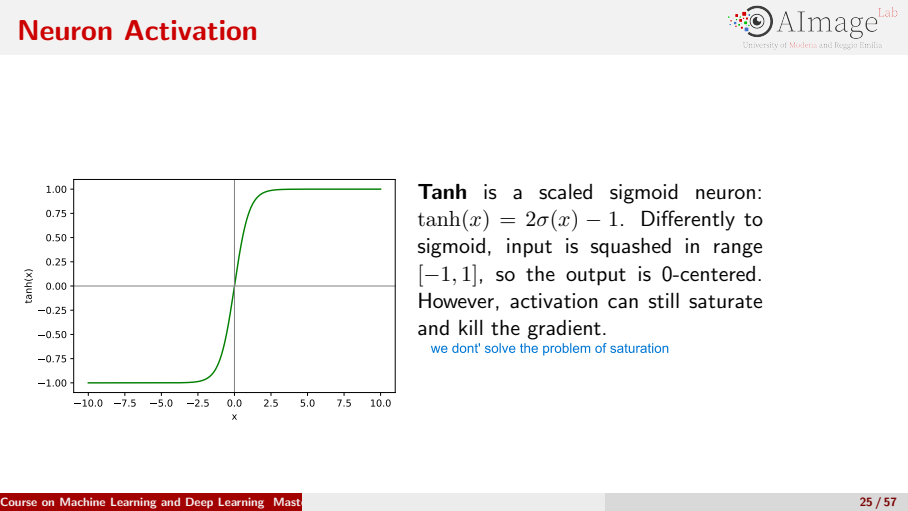
\includegraphics[keepaspectratio]{figure/fig_81a3e54a2f3013db.png}}
\caption{Slide 25 -- Tanh}
\end{figure}
% END F01-B0132

% BEGIN F01-B0133
L\textquotesingle uscita è \textbf{centrata sullo zero}, ma la funzione \textbf{satura ancora}: la sua derivata \(1-\tanh^2(x)\) vale al massimo 1 in \(x=0\) e tende a 0 per \(|x|\) grande. La tanh risolve il primo difetto della sigmoide, non il secondo.
% END F01-B0133

% BEGIN F01-B0134
\begin{quote}
\textbf{Errata slide 25}
\end{quote}
% END F01-B0134

% BEGIN F01-B0135
\begin{quote}
La slide scrive \(\tanh(x) = 2\sigma(x) - 1\). L\textquotesingle identità esatta è \(\tanh(x) = 2\sigma(2x) - 1\) (con \(2\sigma(x)-1\) si ottiene \(\tanh(x/2)\); per \(x = 0.7\): \(\tanh(0.7) = 0.604\), mentre \(2\sigma(0.7)-1 = 0.336\)). Il concetto non cambia: è una sigmoide riscalata e centrata.
\end{quote}
% END F01-B0135

% BEGIN F01-B0136
\subsubsection{ReLU (Rectified Linear Unit)}\label{f01-r386}
% END F01-B0136

% BEGIN F01-B0137
\begin{center}
\begin{adjustbox}{max width=\linewidth}
$\displaystyle 
\boxed{\text{ReLU}(x) = \max(0, x)}, \qquad \frac{d}{dx}\text{ReLU}(x) = \begin{cases}1 & x>0\\ 0 & x<0\end{cases}
$
\end{adjustbox}
\end{center}
% END F01-B0137

% BEGIN F01-B0138
\begin{figure}[H]
\centering
\pandocbounded{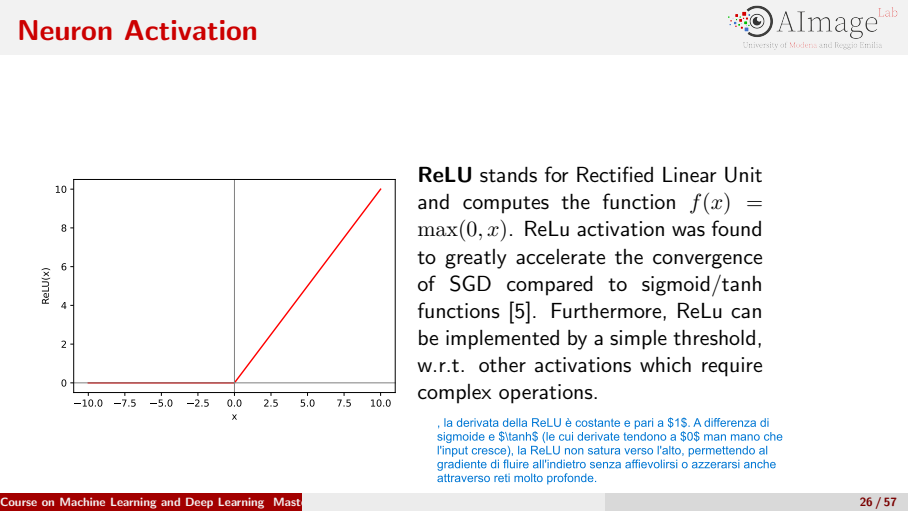
\includegraphics[keepaspectratio]{figure/fig_4c29b6d91b85f692.png}}
\caption{Slide 26 -- ReLU}
\end{figure}
% END F01-B0138

% BEGIN F01-B0139
La ReLU evita la saturazione sul semiasse positivo:
% END F01-B0139

% BEGIN F01-B0140
\begin{itemize}
\tightlist
\item
  nel \textbf{semipiano sinistro} il neurone è \textbf{spento} (uscita 0);
\item
  nel \textbf{semipiano destro} il neurone \textbf{copia} l\textquotesingle ingresso.
\end{itemize}
% END F01-B0140

% BEGIN F01-B0141
Proprietà principali:
% END F01-B0141

% BEGIN F01-B0142
\begin{itemize}
\tightlist
\item
  \textbf{Non satura verso l\textquotesingle alto.} Per \(x>0\) la derivata è 1: questo fattore non attenua il gradiente. I pesi degli altri strati possono comunque amplificarlo o ridurlo, quindi non è una garanzia contro ogni problema di gradiente.
\end{itemize}
% END F01-B0142

% BEGIN F01-B0143
\begin{quote}
\textbf{Precisazione}
\end{quote}
% END F01-B0143

% BEGIN F01-B0144
\begin{quote}
La ReLU è \textbf{continua} in 0 ma \textbf{non derivabile} in 0 (spigolo). La non linearità deriva dallo spigolo, non da una discontinuità. In pratica in \(x = 0\) si usa per convenzione derivata 0.
\end{quote}
% END F01-B0144

% BEGIN F01-B0145
\subsection{Perché servono le non linearità (slide 27)}\label{f01-r406}
% END F01-B0145

% BEGIN F01-B0146
Viene spontaneo chiedersi perché non togliere l\textquotesingle attivazione e usare solo \(Wx\): non satura ed è centrata sullo zero. Il problema è che \textbf{la composizione di funzioni lineari è lineare}.
% END F01-B0146

% BEGIN F01-B0147
\begin{enumerate}
\def\labelenumi{\arabic{enumi}.}
\tightlist
\item
  Con due strati e attivazioni la rete è \(f(x) = \phi\big(W_2\,\phi(W_1 x)\big)\).
\item
  Si tolgono le attivazioni: \(f(x) = W_2 (W_1 x)\).
\item
  Per l\textquotesingle associatività del prodotto matriciale, \(W_2 (W_1 x) = (W_2 W_1)x\).
\item
  \(W_2 W_1\) è \textbf{un\textquotesingle unica matrice}: con \(W_1\in\mathbb{R}^{H\times D}\) e \(W_2\in\mathbb{R}^{K\times H}\), si ha \(W = W_2W_1 \in \mathbb{R}^{K\times D}\). Quindi \(f(x) = Wx\).
\end{enumerate}
% END F01-B0147

% BEGIN F01-B0148
Qualunque sia il numero di strati, senza attivazioni tutta la rete \textbf{collassa in un singolo strato lineare}, cioè in una mappa affine se sono presenti bias. Si ottiene regressione logistica solo conservando una sigmoide o softmax finale. Le attivazioni, essendo non lineari (ReLU compresa), \textbf{impediscono questa fattorizzazione}: sono loro a dare senso alla profondità.
% END F01-B0148

% BEGIN F01-B0149
\begin{center}\rule{0.5\linewidth}{0.5pt}\end{center}
% END F01-B0149

% BEGIN F01-B0150
\section{Reti neurali: il Multilayer Perceptron}\label{f01-r419}
% END F01-B0150

% BEGIN F01-B0151
\subsection{Struttura a strati (slide 29)}\label{f01-r421}
% END F01-B0151

% BEGIN F01-B0152
Connettendo un insieme di neuroni in un grafo si ottiene un \textbf{Multilayer Perceptron (MLP)}. I neuroni sono organizzati in \textbf{strati} (\emph{layer}):
% END F01-B0152

% BEGIN F01-B0153
\begin{itemize}
\tightlist
\item
  \textbf{input layer}: un cerchio per ogni feature d\textquotesingle ingresso. Sono \textbf{cerchi fittizi}: nessun peso, nessuna attivazione, \textbf{nessun parametro};
\item
  \textbf{N hidden layer} nel mezzo;
\item
  \textbf{output layer}: \textbf{un cerchio per ogni classe}, ciascuno dà lo score della sua classe.
\end{itemize}
% END F01-B0153

% BEGIN F01-B0154
Le connessioni sono \textbf{fully connected}:
% END F01-B0154

% BEGIN F01-B0155
\begin{itemize}
\tightlist
\item
  \textbf{nessuna connessione tra neuroni dello stesso strato};
\item
  ogni neurone di uno strato è connesso a \textbf{tutti} i neuroni dello strato successivo;
\item
  ogni connessione è una \textbf{sinapsi}, cioè un peso \(w\).
\end{itemize}
% END F01-B0155

% BEGIN F01-B0156
\begin{figure}[H]
\centering
\pandocbounded{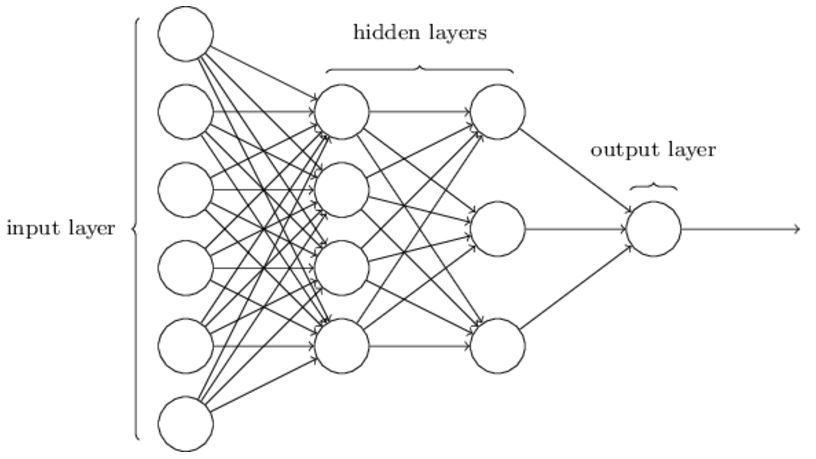
\includegraphics[keepaspectratio]{figure/fig_de29cb90415415c5.jpg}}
\caption{Slide 29 -- MLP con 47 parametri}
\end{figure}
% END F01-B0156

% BEGIN F01-B0157
\textbf{L\textquotesingle equazione di un layer è esattamente il classificatore lineare di §2}, seguito dall\textquotesingle attivazione. La matrice \(W\) ha:
% END F01-B0157

% BEGIN F01-B0158
\begin{itemize}
\tightlist
\item
  \textbf{numero di colonne = numero di feature in ingresso} (\emph{inbound});
\item
  \textbf{numero di righe = numero di feature in uscita} (\emph{outbound}, cioè i neuroni dello strato).
\end{itemize}
% END F01-B0158

% BEGIN F01-B0159
Ogni neurone ha la sua funzione di attivazione. Nella figura ogni neurone del primo hidden layer riceve 6 pesi e produce un valore, quindi \(W_1\) ha 6 colonne e 4 righe.
% END F01-B0159

% BEGIN F01-B0160
\subsection{Esercizio: da dove vengono i 47 parametri?}\label{f01-r444}
% END F01-B0160

% BEGIN F01-B0161
Ogni cerchio rappresenta una combinazione affine \(w^Tx+b\) seguita da un'attivazione: ogni neurone non di input ha \textbf{un peso per ogni ingresso più un bias}. Il conteggio \(6\cdot4 + 4\cdot3 + 3\cdot1 = 39\) dimentica proprio i bias.
% END F01-B0161

% BEGIN F01-B0162
\begin{longtable}[]{@{}llll@{}}
\toprule\noalign{}
Strato & Pesi & Bias & Totale \\
\midrule\noalign{}
\endhead
\bottomrule\noalign{}
\endlastfoot
Input (6) & -- & -- & 0 \\
Hidden 1 (4) & \(4\times6 = 24\) & 4 & 28 \\
Hidden 2 (3) & \(3\times4 = 12\) & 3 & 15 \\
Output (1) & \(1\times3 = 3\) & 1 & 4 \\
\textbf{Totale} & \textbf{39} & \textbf{8} & \textbf{47} \\
\end{longtable}
% END F01-B0162

% BEGIN F01-B0163
In generale, uno strato con \(d\) ingressi e \(k\) neuroni ha \(k\cdot d + k = k(d+1)\) parametri. Questi conteggi vanno avuti perfettamente chiari, perché le architetture cresceranno molto rapidamente.
% END F01-B0163

% BEGIN F01-B0164
\subsection{Forward propagation (slide 30--31)}\label{f01-r458}
% END F01-B0164

% BEGIN F01-B0165
La rete a 4 strati della figura si scrive così, con i bias incorporati nelle matrici \(W\) per alleggerire la notazione:
% END F01-B0165

% BEGIN F01-B0166
\begin{center}
\begin{adjustbox}{max width=\linewidth}
$\displaystyle 
\boxed{\text{out} = \phi\Big(W_3\,\phi\big(W_2\,\phi(W_1 x)\big)\Big)}
$
\end{adjustbox}
\end{center}
% END F01-B0166

% BEGIN F01-B0167
con \(x \in \mathbb{R}^6\), \(W_1 \in \mathbb{R}^{4\times6}\), \(W_2 \in \mathbb{R}^{3\times4}\), \(W_3 \in \mathbb{R}^{1\times3}\). Esplicitando i bias, strato per strato:
% END F01-B0167

% BEGIN F01-B0168
\begin{longtable}[]{@{}lll@{}}
\toprule\noalign{}
Passo & Calcolo & Forma \\
\midrule\noalign{}
\endhead
\bottomrule\noalign{}
\endlastfoot
1 & \(h_1 = \phi(W_1x + b_1)\) & \((4\times6)(6) + (4) \to 4\) \\
2 & \(h_2 = \phi(W_2h_1 + b_2)\) & \((3\times4)(4) + (3) \to 3\) \\
3 & \(\text{out} = \phi(W_3h_2 + b_3)\) & \((1\times3)(3) + (1) \to 1\) \\
\end{longtable}
% END F01-B0168

% BEGIN F01-B0169
\begin{quote}
\textbf{Errata slide 30}
\end{quote}
% END F01-B0169

% BEGIN F01-B0170
\begin{quote}
La slide chiama tutte le matrici \(W_1\) e indica \(W_2\in\mathbb{R}^{4\times3}\). Seguendo la regola "righe = outbound, colonne = inbound", le dimensioni corrette sono \textbf{\(W_2 \in \mathbb{R}^{3\times4}\)} e \textbf{\(W_3 \in \mathbb{R}^{1\times3}\)}.
\end{quote}
% END F01-B0170

% BEGIN F01-B0171
La \textbf{forward propagation} è il calcolo dell\textquotesingle uscita della rete dato l\textquotesingle ingresso. Si chiama \emph{forward} perché segue il flusso dell\textquotesingle informazione \textbf{dall\textquotesingle input verso la risposta}, ad esempio dall\textquotesingle immagine alla sua classe.
% END F01-B0171

% BEGIN F01-B0172
\begin{figure}[H]
\centering
\pandocbounded{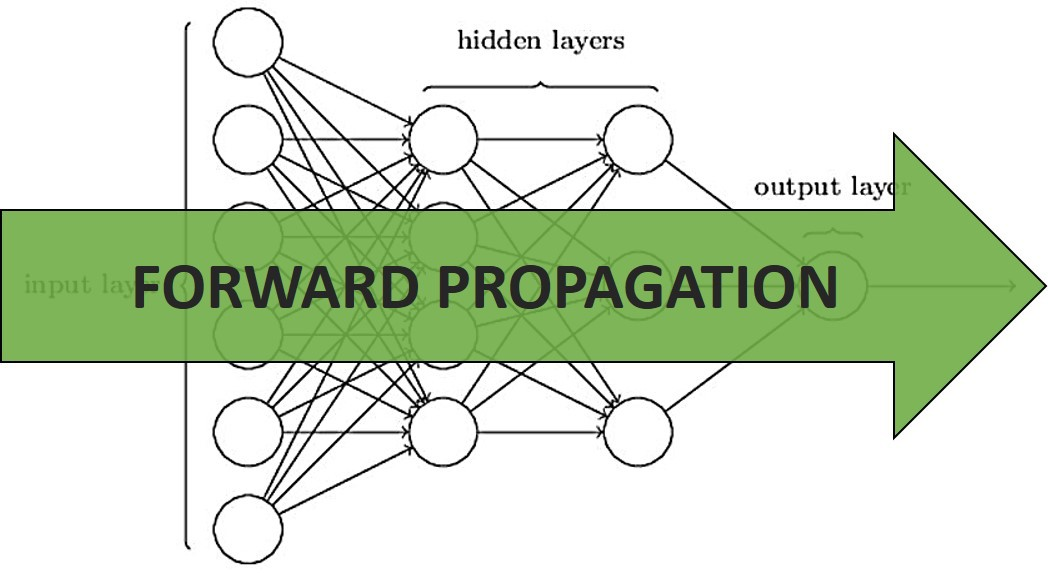
\includegraphics[keepaspectratio]{figure/fig_568c3a2a50b4a77d.jpg}}
\caption{Slide 31 -- Forward propagation}
\end{figure}
% END F01-B0172

% BEGIN F01-B0173
Una rete neurale è quindi una \textbf{composizione non lineare di tante unità lineari}, cioè una grande composizione di funzioni.
% END F01-B0173

% BEGIN F01-B0174
Le equazioni rendono esplicito il calcolo della rete. Questo non rende automaticamente interpretabili le rappresentazioni apprese: conoscere le operazioni e attribuire un significato semantico a ogni feature sono problemi distinti.
% END F01-B0174

% BEGIN F01-B0175
\begin{center}\rule{0.5\linewidth}{0.5pt}\end{center}
% END F01-B0175

% BEGIN F01-B0176
\section{Potere rappresentazionale}\label{f01-r487}
% END F01-B0176

% BEGIN F01-B0177
Nella formula compatta senza bias questi sono \textbf{omessi}, non incorporati nelle matrici delle dimensioni riportate. Per incorporarli bisogna aumentare l\textquotesingle ingresso di una componente costante e aggiungere una colonna a ogni matrice: \([W\ b][h^T\ 1]^T=Wh+b\).
% END F01-B0177

% BEGIN F01-B0178
\subsection{Il teorema di approssimazione universale (slide 32)}\label{f01-r491}
% END F01-B0178

% BEGIN F01-B0179
Una rete è fatta solo di prodotti scalari, somme e soglie. Che percentuale di "tutte le funzioni del mondo", anche quelle non ancora scoperte, può rappresentare?
% END F01-B0179

% BEGIN F01-B0180
\begin{quote}
\textbf{Teorema di approssimazione universale (slide 32)}
\end{quote}
% END F01-B0180

% BEGIN F01-B0181
\begin{quote}
Siano \(K\subset\mathbb{R}^d\) compatto e \(f:K\to\mathbb{R}\) continua. Con un\textquotesingle attivazione adatta, per esempio sigmoide, per ogni \(\epsilon>0\) esiste una rete con uno strato nascosto sufficientemente ampio tale che \begin{center}
\begin{adjustbox}{max width=\linewidth}
$\displaystyle \boxed{\sup_{x\in K}|f(x)-g(x)|<\epsilon.}$
\end{adjustbox}
\end{center} Una forma della rete è \(g(x)=\sum_{j=1}^{m}a_j\sigma(w_j^Tx+b_j)+c\), con \(w_j\in\mathbb{R}^d\) e gli altri coefficienti scalari.
\end{quote}
% END F01-B0181

% BEGIN F01-B0182
La precisione è uniforme su \(K\): vale per ogni suo punto, non soltanto in media sui campioni. Il numero \(m\) può dipendere dalla funzione e dalla precisione richiesta. L\textquotesingle enunciato non promette un\textquotesingle approssimazione uniforme sull\textquotesingle intero spazio non limitato, né dice che qualunque attivazione o qualunque rete piccola siano sufficienti. Non permette di dedurre la prevedibilità di fenomeni casuali o l\textquotesingle esistenza di informazioni assenti dall\textquotesingle input.
% END F01-B0182

% BEGIN F01-B0183
Per esempio, approssimare una funzione su \([0,1]\) con errore inferiore a \(0.01\) significa mantenere tutta la curva della rete nella fascia verticale \(f(x)\pm0.01\). È una proprietà di rappresentazione, non un algoritmo per trovare i pesi.
% END F01-B0183

% BEGIN F01-B0184
\textbf{Rappresentare non significa imparare bene.} Il teorema dice che lo strumento \emph{può} rappresentare la funzione, non che la imparerà. È come chiedersi "sei fisicamente in grado di giocare a calcio?": sì. "Sei un buon giocatore?": dipende dall\textquotesingle allenamento. Il teorema riguarda la \textbf{rappresentazione}, non la \textbf{performance}.
% END F01-B0184

% BEGIN F01-B0185
\subsection{Dalla teoria alla pratica}\label{f01-r506}
% END F01-B0185

% BEGIN F01-B0186
Passando dalla matematica al computer si introducono approssimazioni:
% END F01-B0186

% BEGIN F01-B0187
\begin{enumerate}
\def\labelenumi{\arabic{enumi}.}
\tightlist
\item
  nel computer funzioni e numeri \textbf{non sono continui ma discreti} (precisione finita);
\item
  anche le \textbf{misure} degli strumenti sono discrete (risoluzione finita).
\end{enumerate}
% END F01-B0187

% BEGIN F01-B0188
Una capacità sufficiente permette di rappresentare relazioni complesse; più profondità può rappresentarle in modo più efficiente. Aumentare la dimensione, però, non garantisce prestazioni migliori: contano dati, ottimizzazione e regolarizzazione. La precisione finita non dimostra che una rete più grande sia sempre preferibile.
% END F01-B0188

% BEGIN F01-B0189
\begin{center}\rule{0.5\linewidth}{0.5pt}\end{center}
% END F01-B0189

% BEGIN F01-B0190
\section{Iperparametri e overfitting}\label{f01-r517}
% END F01-B0190

% BEGIN F01-B0191
\subsection{Iperparametri dell\textquotesingle architettura (slide 33)}\label{f01-r519}
% END F01-B0191

% BEGIN F01-B0192
Numero di layer e numero di neuroni per layer sono \textbf{iperparametri} dell\textquotesingle architettura:
% END F01-B0192

% BEGIN F01-B0193
\begin{itemize}
\tightlist
\item
  aumentarli fa \textbf{crescere la capacità} della rete, cioè lo spazio delle funzioni rappresentabili (\textbf{bene});
\item
  reti più grandi \textbf{senza regolarizzazione} sono molto più inclini all\textquotesingle{}\textbf{overfitting} (\textbf{male}).
\end{itemize}
% END F01-B0193

% BEGIN F01-B0194
\subsection{Perché le reti tendono a fare overfitting}\label{f01-r526}
% END F01-B0194

% BEGIN F01-B0195
Durante l\textquotesingle addestramento si dà alla rete solo una \textbf{loss} da ottimizzare sul training set, chiedendole di risolverla al meglio. Con molti parametri la rete ha \textbf{molti "posti" in cui memorizzare il training set}: questo è l\textquotesingle overfitting.
% END F01-B0195

% BEGIN F01-B0196
La sovraparametrizzazione rende possibile memorizzare il training set, ma non implica necessariamente overfitting. Il problema è una discrepanza tra buone prestazioni di training e prestazioni peggiori su dati nuovi: si valuta con un insieme di validazione indipendente.
% END F01-B0196

% BEGIN F01-B0197
L'overfitting è una causa di scarsa generalizzazione anche quando il training è ben ottimizzato e va tenuto sempre presente.
% END F01-B0197

% BEGIN F01-B0198
\begin{figure}[H]
\centering
\pandocbounded{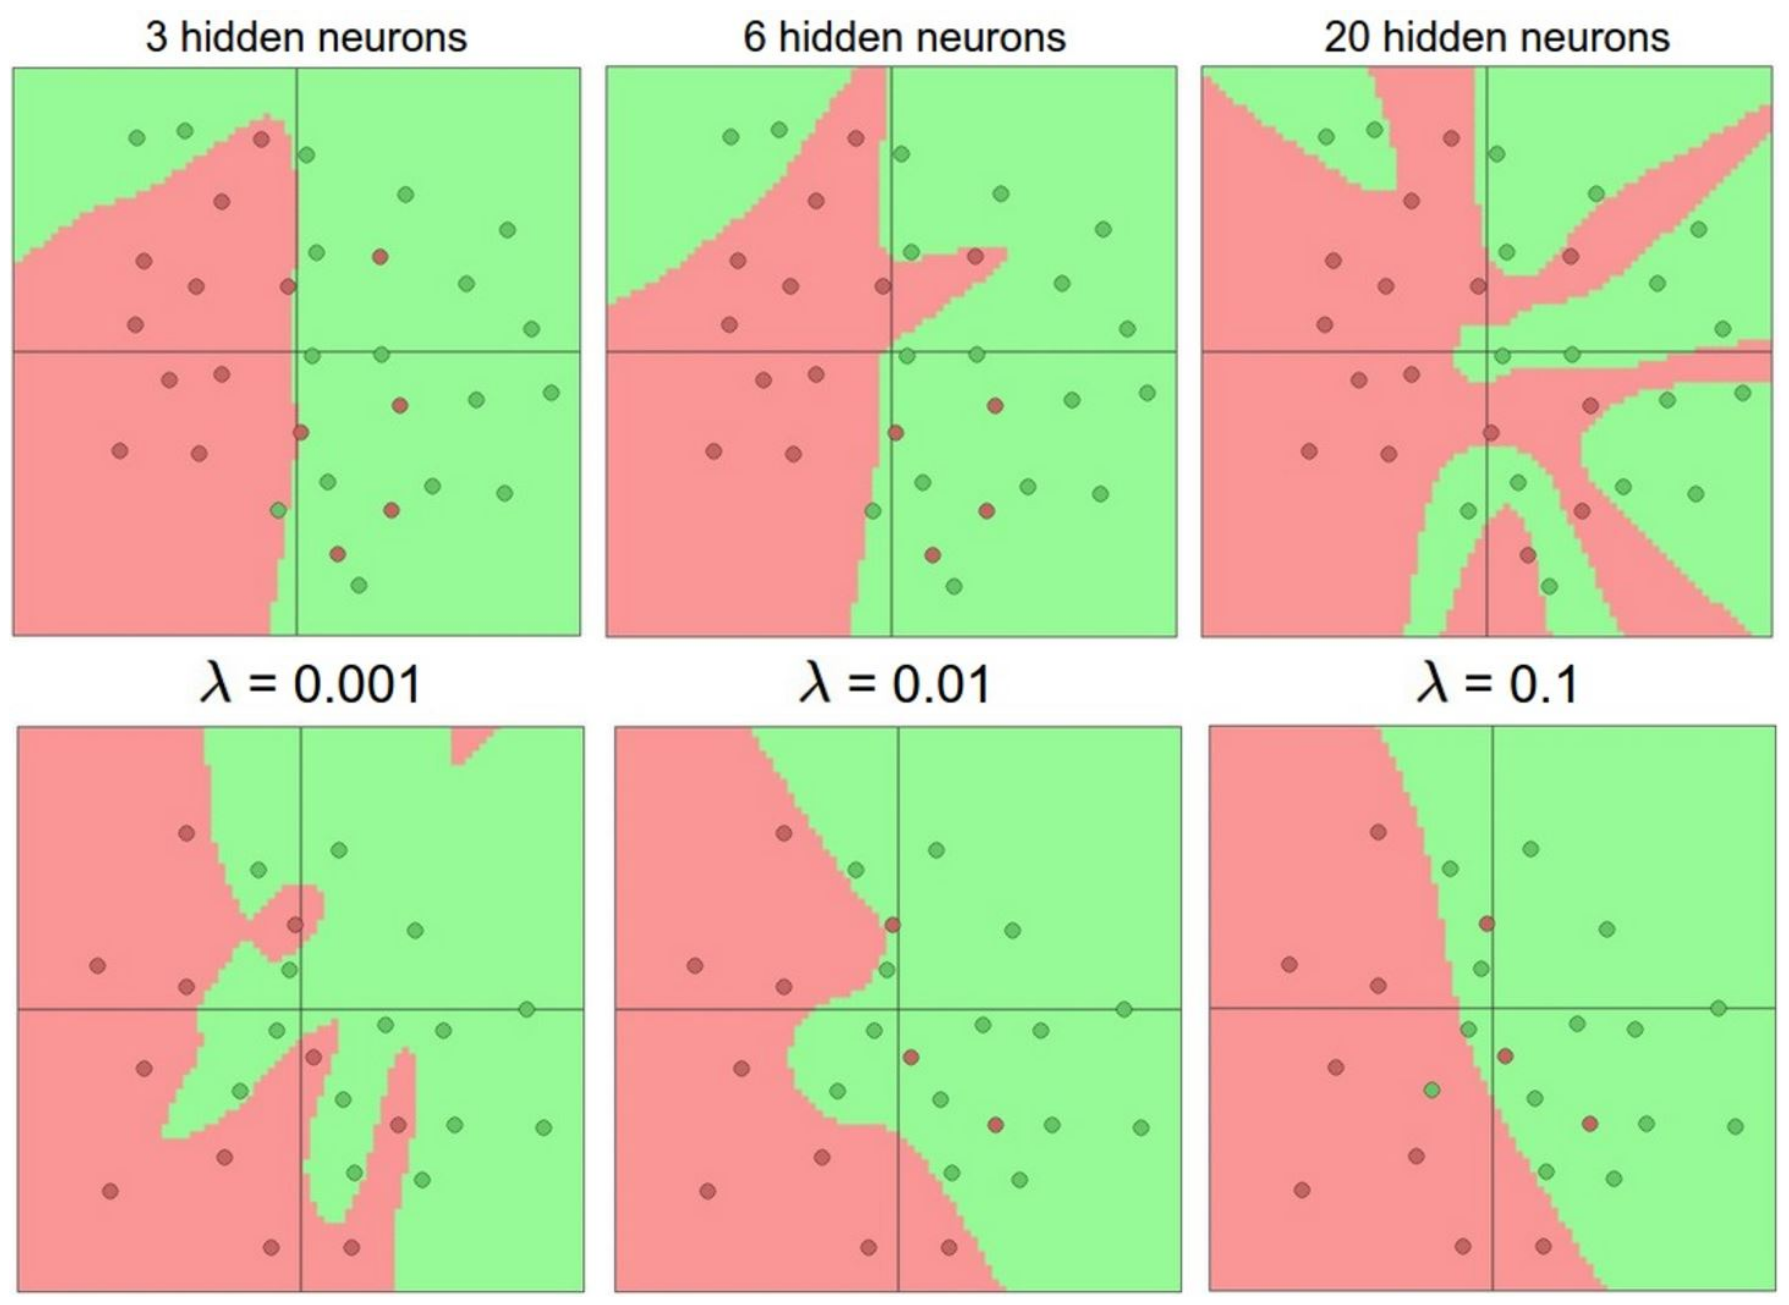
\includegraphics[keepaspectratio]{figure/fig_711961814de58055.png}}
\caption{Slide 34 -- Superfici di decisione al variare dei neuroni e di λ}
\end{figure}
% END F01-B0198

% BEGIN F01-B0199
\textbf{Riga superiore (slide 34).} Rete a 3 layer che separa punti rossi e verdi, al variare del numero di neuroni nascosti:
% END F01-B0199

% BEGIN F01-B0200
\begin{itemize}
\tightlist
\item
  \textbf{3 neuroni}: superficie non lineare ma regolare;
\item
  \textbf{6 neuroni}: compaiono forme irregolari;
\item
  \textbf{20 neuroni}: superficie molto irregolare, con zone rosse attorno a singoli punti che probabilmente sarebbero verdi. Aumentando ancora, la rete finirebbe per \textbf{disegnare un cerchio attorno a ogni punto}.
\end{itemize}
% END F01-B0200

% BEGIN F01-B0201
Una frontiera molto irregolare può suggerire overfitting, che va verificato su dati indipendenti. E 20 neuroni sono pochissimi.
% END F01-B0201

% BEGIN F01-B0202
\textbf{Regola pratica (slide 34).} Le reti si fanno \textbf{grandi quanto consente il budget computazionale}, e poi si previene l\textquotesingle overfitting con opportune \textbf{tecniche di regolarizzazione} (dropout, weight decay, input noise\ldots), viste in §7.4 e §10.
% END F01-B0202

% BEGIN F01-B0203
\begin{center}\rule{0.5\linewidth}{0.5pt}\end{center}
% END F01-B0203

% BEGIN F01-B0204
\section{Addestrare una rete: funzione obiettivo e loss}\label{f01-r548}
% END F01-B0204

% BEGIN F01-B0205
\subsection{La funzione obiettivo (slide 36)}\label{f01-r550}
% END F01-B0205

% BEGIN F01-B0206
Con l\textquotesingle architettura si è definita una \textbf{funzione parametrica}, la forward propagation. Ora serve una procedura per \textbf{imparare i parametri}, esattamente come per qualunque modello parametrico di ML: si definisce una loss e la si minimizza.
% END F01-B0206

% BEGIN F01-B0207
La loss deve essere un \textbf{surrogato continuo} del problema da risolvere: cross-entropy per la classificazione, MSE per la regressione, ecc. Valgono tutte le considerazioni di ML già viste: \textbf{l\textquotesingle ipotesi i.i.d.}, il modo di campionare i dati, la \textbf{partizione training/test}, la variabilità del training set.
% END F01-B0207

% BEGIN F01-B0208
La funzione obiettivo misura la \textbf{qualità della mappatura} input → output e ha due termini:
% END F01-B0208

% BEGIN F01-B0209
\begin{center}
\begin{adjustbox}{max width=\linewidth}
$\displaystyle 
\boxed{\mathcal{L}(\theta; x, y) = \underbrace{\frac{1}{N}\sum_{i=1}^{N} L_i(\theta; x_i, y_i)}_{\text{data term}} + \underbrace{\lambda\,\Omega(\theta)}_{\text{regularization term}}}
$
\end{adjustbox}
\end{center}
% END F01-B0209

% BEGIN F01-B0210
\begin{longtable}[]{@{}
  >{\raggedright\arraybackslash}p{(\linewidth - 2\tabcolsep) * \real{0.5000}}
  >{\raggedright\arraybackslash}p{(\linewidth - 2\tabcolsep) * \real{0.5000}}@{}}
\toprule\noalign{}
\begin{minipage}[b]{\linewidth}\raggedright
Simbolo
\end{minipage} & \begin{minipage}[b]{\linewidth}\raggedright
Significato
\end{minipage} \\
\midrule\noalign{}
\endhead
\bottomrule\noalign{}
\endlastfoot
\(N\) & numero di esempi di training \\
\(\theta\) & insieme di \textbf{tutti} i parametri della rete: \(\{W_1, b_1, W_2, b_2, \dots\}\) \\
\(L_i\) & loss del singolo esempio \(i\) \\
\(\Omega(\theta)\) & regolarizzatore \\
\(\lambda \ge 0\) & \textbf{forza} della regolarizzazione \\
\end{longtable}
% END F01-B0210

% BEGIN F01-B0211
\begin{itemize}
\tightlist
\item
  \textbf{Data term.} Dipende dai \textbf{parametri}, dagli \textbf{input} e dalla \textbf{ground truth}. È una media sugli esempi e misura quanto sono buone le predizioni rispetto alle etichette; dipende dal problema (classificazione o regressione).
\item
  \textbf{Regularization term.} Dipende \textbf{solo dai parametri}: non dall\textquotesingle input, non dall\textquotesingle output, non dalla bontà delle predizioni. Impone un \textbf{vincolo strutturale} sui pesi: chiede di risolvere il problema \textbf{usando i parametri il meno possibile}, e così riduce il rischio di overfitting.
\end{itemize}
% END F01-B0211

% BEGIN F01-B0212
\begin{figure}[H]
\centering
\pandocbounded{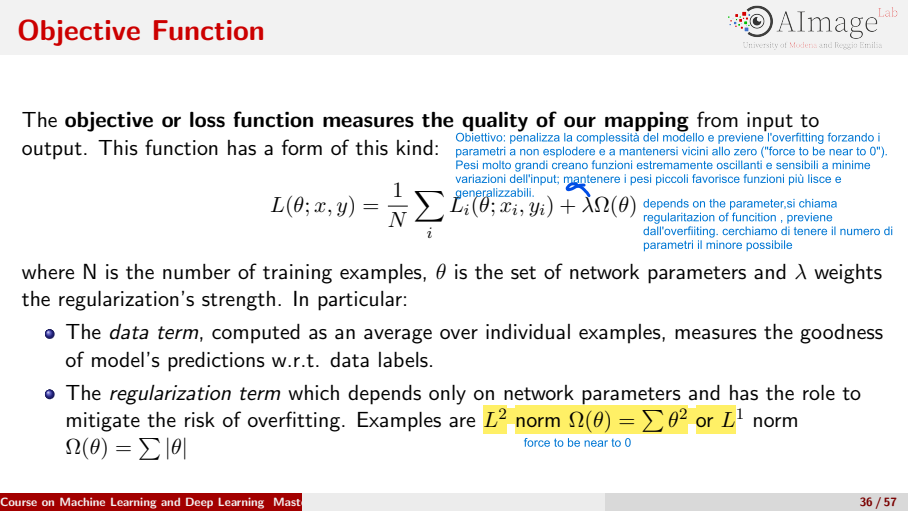
\includegraphics[keepaspectratio]{figure/fig_a6013aed45ce7bd3.png}}
\caption{Slide 36 -- Funzione obiettivo, con annotazioni}
\end{figure}
% END F01-B0212

% BEGIN F01-B0213
\subsection{Le loss più usate (slide 37)}\label{f01-r575}
% END F01-B0213

% BEGIN F01-B0214
Le funzioni di loss sono moltissime, ma circa il 90\% dei problemi usa quelle della slide 37. La maggior parte delle loss moderne sono loro \textbf{piccole modifiche}.
% END F01-B0214

% BEGIN F01-B0215
\begin{figure}[H]
\centering
\pandocbounded{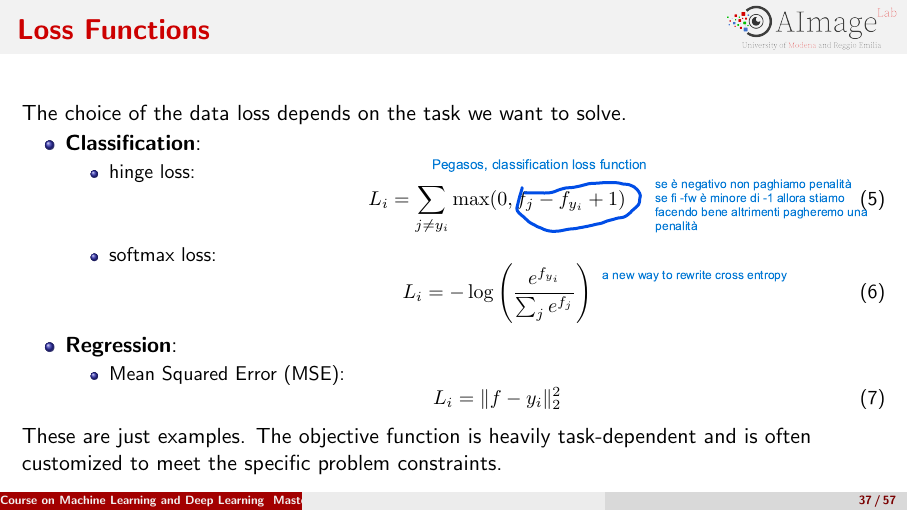
\includegraphics[keepaspectratio]{figure/fig_5fd355097a7cb78b.png}}
\caption{Slide 37 -- Loss functions, con annotazioni}
\end{figure}
% END F01-B0215

% BEGIN F01-B0216
Notazione: \(f = f(x_i;\theta) \in \mathbb{R}^K\) è il vettore degli score prodotti dalla rete per l\textquotesingle esempio \(i\), \(f_j\) lo score della classe \(j\), \(y_i\) l\textquotesingle indice della classe corretta.
% END F01-B0216

% BEGIN F01-B0217
\subsubsection{Hinge loss (classificazione)}\label{f01-r583}
% END F01-B0217

% BEGIN F01-B0218
\begin{center}
\begin{adjustbox}{max width=\linewidth}
$\displaystyle 
\boxed{L_i = \sum_{j\neq y_i}\max\big(0,\; f_j - f_{y_i} + 1\big)}
$
\end{adjustbox}
\end{center}
% END F01-B0218

% BEGIN F01-B0219
È la loss della \textbf{SVM lineare} (algoritmo \emph{Pegasos}). Si chiede al classificatore non solo di classificare correttamente, ma di farlo con un \textbf{margine}: lo score della classe corretta deve superare quello di \textbf{ogni} altra classe di almeno 1.
% END F01-B0219

% BEGIN F01-B0220
\textbf{Come funziona, passo passo.} Per ogni classe sbagliata \(j\):
% END F01-B0220

% BEGIN F01-B0221
\begin{enumerate}
\def\labelenumi{\arabic{enumi}.}
\tightlist
\item
  si calcola \(f_j - f_{y_i} + 1\);
\item
  se \(f_{y_i} \ge f_j + 1\), cioè la classe giusta batte la \(j\) con margine almeno 1, la quantità è \(\le 0\) e il \(\max\) restituisce \textbf{0: nessuna penalità};
\item
  altrimenti la quantità è positiva e si \textbf{paga una penalità proporzionale} a quanto manca per raggiungere il margine;
\item
  si sommano i contributi di tutte le classi sbagliate.
\end{enumerate}
% END F01-B0221

% BEGIN F01-B0222
(Annotazione slide 37: \emph{"se è negativo non paghiamo penalità; se \(f_j - f_{y_i}\) è minore di −1 allora stiamo facendo bene, altrimenti pagheremo una penalità"}.)
% END F01-B0222

% BEGIN F01-B0223
\textbf{Esempio con gli score della slide 15}, \(f = [-96.8,\ 437.9,\ 60.75]\) (gatto, cane, nave):
% END F01-B0223

% BEGIN F01-B0224
\begin{longtable}[]{@{}
  >{\raggedright\arraybackslash}p{(\linewidth - 4\tabcolsep) * \real{0.3333}}
  >{\raggedright\arraybackslash}p{(\linewidth - 4\tabcolsep) * \real{0.3333}}
  >{\raggedright\arraybackslash}p{(\linewidth - 4\tabcolsep) * \real{0.3333}}@{}}
\toprule\noalign{}
\begin{minipage}[b]{\linewidth}\raggedright
Classe vera
\end{minipage} & \begin{minipage}[b]{\linewidth}\raggedright
Termini della somma
\end{minipage} & \begin{minipage}[b]{\linewidth}\raggedright
\(L_i\)
\end{minipage} \\
\midrule\noalign{}
\endhead
\bottomrule\noalign{}
\endlastfoot
gatto & \(\max(0,\ 437.9+96.8+1) + \max(0,\ 60.75+96.8+1) = 535.7 + 158.55\) & \textbf{694.25} \\
cane & \(\max(0,\ -96.8-437.9+1) + \max(0,\ 60.75-437.9+1) = 0 + 0\) & \textbf{0} \\
\end{longtable}
% END F01-B0224

% BEGIN F01-B0225
Se l\textquotesingle immagine è un gatto il classificatore paga molto. Se fosse un cane la loss sarebbe nulla, perché "cane" batte le altre classi con ampio margine.
% END F01-B0225

% BEGIN F01-B0226
È la stessa idea del margine della SVM, dove si chiede una distanza minima tra l\textquotesingle iperplano di separazione e le due classi. Qui però il margine non è imposto con un \textbf{vincolo}, ma tramite una sua versione "morbida" e linearizzata, il \(\max(0,\cdot)\).
% END F01-B0226

% BEGIN F01-B0227
\textbf{Perché proprio 1?} La riscalatura del margine richiede anche di adattare il peso relativo della regolarizzazione per mantenere lo stesso problema. Qualunque altro margine \(\Delta > 0\) (10, 20, 300\ldots) sarebbe equivalente, perché può essere \textbf{assorbito nella norma dei parametri}:
% END F01-B0227

% BEGIN F01-B0228
\begin{enumerate}
\def\labelenumi{\arabic{enumi}.}
\tightlist
\item
  moltiplicando per \(c > 0\) i pesi e il bias dello strato di uscita (in un classificatore lineare, tutti i parametri), tutti gli score si moltiplicano per \(c\): \(f \to c f\);
\item
  quindi anche le differenze si moltiplicano per \(c\): \(f_{y_i} - f_j \to c\,(f_{y_i} - f_j)\);
\item
  se dei parametri garantiscono il margine 1, gli stessi parametri con lo strato di uscita moltiplicato per \(\Delta\) garantiscono il margine \(\Delta\), e viceversa.
\end{enumerate}
% END F01-B0228

% BEGIN F01-B0229
Il valore del margine si ottiene quindi semplicemente cambiando la scala dei pesi. È lo stesso passaggio della SVM, dove il margine \(2\rho\) veniva riportato a 1 assorbendolo in \(w\).
% END F01-B0229

% BEGIN F01-B0230
\subsubsection{Softmax loss / cross-entropy (classificazione)}\label{f01-r619}
% END F01-B0230

% BEGIN F01-B0231
\begin{center}
\begin{adjustbox}{max width=\linewidth}
$\displaystyle 
\boxed{L_i = -\log\left(\frac{e^{f_{y_i}}}{\sum_j e^{f_j}}\right)}
$
\end{adjustbox}
\end{center}
% END F01-B0231

% BEGIN F01-B0232
È la loss più usata, ed è \textbf{un altro modo di scrivere la cross-entropy} (annotazione slide 37: \emph{"a new way to rewrite cross entropy"}). Prende infatti i nomi di \emph{cross-entropy} o \emph{softmax loss}. Anche GPT usa questa loss, in una forma leggermente diversa.
% END F01-B0232

% BEGIN F01-B0233
\textbf{Derivazione dalla cross-entropy, passo passo:}
% END F01-B0233

% BEGIN F01-B0234
\begin{enumerate}
\def\labelenumi{\arabic{enumi}.}
\tightlist
\item
  Si parte dalla cross-entropy di §2.4: \(L_i = -\sum_k y^{true}_k \log y^{pred}_k\).
\item
  \(y^{true}\) è one-hot: vale 1 solo per \(k = y_i\) e 0 altrove. La somma fa quindi da \textbf{selettore}, come nella BCE, e sopravvive un solo termine: \(L_i = -\log y^{pred}_{y_i}\).
\item
  \(y^{pred}\) è la softmax degli score, quindi \(y^{pred}_{y_i} = \dfrac{e^{f_{y_i}}}{\sum_j e^{f_j}}\), da cui la formula nel riquadro.
\item
  Usando \(\log(a/b) = \log a - \log b\) e \(\log e^{a} = a\) si ottiene una forma equivalente, utile per i calcoli: \begin{center}
\begin{adjustbox}{max width=\linewidth}
$\displaystyle L_i = -f_{y_i} + \log\sum_j e^{f_j}$
\end{adjustbox}
\end{center}
\end{enumerate}
% END F01-B0234

% BEGIN F01-B0235
Minimizzare \(-\log(\cdot)\) equivale a \textbf{massimizzare} la probabilità (normalizzata) della classe corretta: si prende lo score della risposta giusta e lo si vuole alzare.
% END F01-B0235

% BEGIN F01-B0236
\textbf{Esempio} con gli score della slide 18, \(z = [1.2,\ 5.1,\ 2.7]\) e softmax \([0.018,\ 0.900,\ 0.082]\):
% END F01-B0236

% BEGIN F01-B0237
\begin{longtable}[]{@{}ll@{}}
\toprule\noalign{}
Classe vera & \(L_i = -\log(\text{softmax}_{y_i})\) \\
\midrule\noalign{}
\endhead
\bottomrule\noalign{}
\endlastfoot
classe 2 (score più alto) & \(-\log 0.900 = 0.105\) \\
classe 3 & \(-\log 0.082 = 2.51\) \\
classe 1 (score più basso) & \(-\log 0.018 = 4.01\) \\
\end{longtable}
% END F01-B0237

% BEGIN F01-B0238
\textbf{Il gradiente della softmax loss.} È il termine \(\partial L/\partial o\) da cui parte la backpropagation (§8.4). Derivando la forma del passo 4 rispetto al generico score \(f_k\):
% END F01-B0238

% BEGIN F01-B0239
\begin{enumerate}
\def\labelenumi{\arabic{enumi}.}
\tightlist
\item
  il termine \(-f_{y_i}\) ha derivata \(-1\) se \(k = y_i\) e \(0\) altrimenti; si scrive \(-\mathbb{1}[k = y_i]\);
\item
  il termine \(\log\sum_j e^{f_j}\) ha derivata \(\dfrac{1}{\sum_j e^{f_j}}\cdot e^{f_k}\) (regola della catena: derivata del log per derivata dell\textquotesingle argomento), cioè proprio \(\text{softmax}_k(f)\);
\item
  quindi: \begin{center}
\begin{adjustbox}{max width=\linewidth}
$\displaystyle \boxed{\frac{\partial L_i}{\partial f_k} = \text{softmax}_k(f) - \mathbb{1}[k = y_i]}$
\end{adjustbox}
\end{center}
\end{enumerate}
% END F01-B0239

% BEGIN F01-B0240
Il gradiente è "probabilità predetta meno target": per l\textquotesingle esempio con classe vera 2 vale \([0.018,\ 0.900-1,\ 0.082] = [0.018,\ -0.100,\ 0.082]\). È la stessa forma "predizione − etichetta" della regressione logistica.
% END F01-B0240

% BEGIN F01-B0241
\subsubsection{Mean Squared Error (regressione)}\label{f01-r654}
% END F01-B0241

% BEGIN F01-B0242
\begin{center}
\begin{adjustbox}{max width=\linewidth}
$\displaystyle 
\boxed{L_i = \lVert f - y_i \rVert_2^2 = \sum_k \big(f_k - y_{i,k}\big)^2}
$
\end{adjustbox}
\end{center}
% END F01-B0242

% BEGIN F01-B0243
Nella regressione si conoscono coppie di input e output di una funzione, ma non la sua forma né la sua equazione, e la si vuole "indovinare" a meno di una certa approssimazione. Nella regressione lineare la funzione cercata era lineare; con una rete neurale non lo è. La loss più usata, nella sua forma base, è l\textquotesingle errore quadratico: si prende la differenza tra predizione e target e la si eleva al quadrato.
% END F01-B0243

% BEGIN F01-B0244
Ad esempio, con predizione \(2.5\) e target \(2\) si ha \(L_i = 0.25\). Il gradiente rispetto alla predizione è \(2(f - y_i)\), cioè di nuovo proporzionale all\textquotesingle errore.
% END F01-B0244

% BEGIN F01-B0245
\begin{quote}
\textbf{Le loss dipendono dal compito}
\end{quote}
% END F01-B0245

% BEGIN F01-B0246
\begin{quote}
Queste sono le famiglie principali. La funzione obiettivo dipende molto dal compito e spesso la si personalizza, con termini aggiuntivi o una forma adattata alle particolarità del problema.
\end{quote}
% END F01-B0246

% BEGIN F01-B0247
\subsection{Imparare i parametri (slide 38)}\label{f01-r667}
% END F01-B0247

% BEGIN F01-B0248
Durante il training si cerca l\textquotesingle insieme di parametri che \textbf{minimizza la funzione obiettivo} (data term + regolarizzazione) sul training set:
% END F01-B0248

% BEGIN F01-B0249
\begin{center}
\begin{adjustbox}{max width=\linewidth}
$\displaystyle 
\boxed{\theta^* = \arg\min_\theta \left( \frac{1}{N}\sum_i L_i(\theta; x_i, y_i) + \lambda\,\Omega(\theta) \right)}
$
\end{adjustbox}
\end{center}
% END F01-B0249

% BEGIN F01-B0250
Lo si fa con la discesa del gradiente, \(\theta \leftarrow \theta - \eta\,\nabla_\theta\mathcal{L}\). Serve quindi la derivata della loss rispetto a \textbf{ogni} parametro di \textbf{ogni} strato, ed è questo il compito della backpropagation (§8).
% END F01-B0250

% BEGIN F01-B0251
\subsection{\texorpdfstring{Regolarizzazione esplicita: \(L_2\) e \(L_1\) (slide 36)}{Regolarizzazione esplicita: L\_2 e L\_1 (slide 36)}}\label{f01-r677}
% END F01-B0251

% BEGIN F01-B0252
\textbf{Quadrato della norma \(L_2\)} (equivalente a decadimento dei pesi nella discesa del gradiente semplice):
% END F01-B0252

% BEGIN F01-B0253
\begin{center}
\begin{adjustbox}{max width=\linewidth}
$\displaystyle 
\Omega(\theta) = \sum_j \theta_j^2, \qquad \frac{\partial\Omega}{\partial\theta_j} = 2\theta_j
$
\end{adjustbox}
\end{center}
% END F01-B0253

% BEGIN F01-B0254
È minima quando i parametri sono \textbf{nulli o piccoli}. Essendo una funzione liscia, \textbf{non forza i parametri a essere esattamente zero, ma li rende piccoli} (\emph{"force to be near to 0"}). Pesi molto grandi producono funzioni oscillanti e sensibili a minime variazioni dell\textquotesingle input; pesi piccoli favoriscono funzioni \textbf{più lisce e generalizzabili} (annotazione slide 36).
% END F01-B0254

% BEGIN F01-B0255
\textbf{Norma \(L_1\):}
% END F01-B0255

% BEGIN F01-B0256
\begin{center}
\begin{adjustbox}{max width=\linewidth}
$\displaystyle 
\Omega(\theta) = \sum_j |\theta_j|, \qquad \frac{\partial\Omega}{\partial\theta_j} = \operatorname{sign}(\theta_j)\quad(\theta_j \neq 0)
$
\end{adjustbox}
\end{center}
% END F01-B0256

% BEGIN F01-B0257
La derivata ha modulo \textbf{1 per ogni parametro non nullo}, indipendentemente da quanto è piccolo. La \(L_1\) è un regolarizzatore di \textbf{sparsità}: favorisce soluzioni con alcuni parametri \textbf{esattamente zero}, ma penalizza la somma dei moduli, non il numero dei coefficienti non nulli.
% END F01-B0257

% BEGIN F01-B0258
\textbf{Da dove viene la differenza: l\textquotesingle aggiornamento passo passo.} Si guarda solo l\textquotesingle effetto del regolarizzatore su un singolo peso \(\theta\), con learning rate \(\eta\).
% END F01-B0258

% BEGIN F01-B0259
\begin{enumerate}
\def\labelenumi{\arabic{enumi}.}
\tightlist
\item
  \textbf{\(L_2\):} \begin{center}
\begin{adjustbox}{max width=\linewidth}
$\displaystyle \theta \leftarrow \theta - \eta\lambda\cdot 2\theta = (1 - 2\eta\lambda)\,\theta$
\end{adjustbox}
\end{center} A ogni passo il peso viene \textbf{moltiplicato} per un fattore tra 0 e 1 quando \(0<2\eta\lambda<1\): decade in proporzione a quanto è grande (da qui il nome \emph{weight decay}). Più è piccolo, più piccola è la spinta.
\item
  \textbf{\(L_1\):} \begin{center}
\begin{adjustbox}{max width=\linewidth}
$\displaystyle \theta \leftarrow \theta - \eta\lambda\,\operatorname{sign}(\theta)$
\end{adjustbox}
\end{center} A ogni passo al peso si \textbf{sottrae} una quantità \textbf{costante}, qualunque sia il suo valore. La spinta non si attenua, ma il metodo a passo costante può oltrepassare zero e oscillare. Per esempio, con passo \(0.1\), \(0.05\to-0.05\to0.05\). La sparsità dell'ottimo non garantisce che un aggiornamento elementare raggiunga esattamente zero. In zero si usa un sottogradiente in \([-1,1]\).
\end{enumerate}
% END F01-B0259

% BEGIN F01-B0260
\textbf{Esempio:} \(\theta = 1\) con \(2\eta\lambda = 0.2\) per \(L_2\) e \(\eta\lambda = 0.1\) per \(L_1\), ignorando il data term.
% END F01-B0260

% BEGIN F01-B0261
\begin{longtable}[]{@{}
  >{\raggedright\arraybackslash}p{(\linewidth - 12\tabcolsep) * \real{0.1429}}
  >{\raggedright\arraybackslash}p{(\linewidth - 12\tabcolsep) * \real{0.1429}}
  >{\raggedright\arraybackslash}p{(\linewidth - 12\tabcolsep) * \real{0.1429}}
  >{\raggedright\arraybackslash}p{(\linewidth - 12\tabcolsep) * \real{0.1429}}
  >{\raggedright\arraybackslash}p{(\linewidth - 12\tabcolsep) * \real{0.1429}}
  >{\raggedright\arraybackslash}p{(\linewidth - 12\tabcolsep) * \real{0.1429}}
  >{\raggedright\arraybackslash}p{(\linewidth - 12\tabcolsep) * \real{0.1429}}@{}}
\toprule\noalign{}
\begin{minipage}[b]{\linewidth}\raggedright
passo
\end{minipage} & \begin{minipage}[b]{\linewidth}\raggedright
0
\end{minipage} & \begin{minipage}[b]{\linewidth}\raggedright
1
\end{minipage} & \begin{minipage}[b]{\linewidth}\raggedright
2
\end{minipage} & \begin{minipage}[b]{\linewidth}\raggedright
3
\end{minipage} & \begin{minipage}[b]{\linewidth}\raggedright
\ldots{}
\end{minipage} & \begin{minipage}[b]{\linewidth}\raggedright
10
\end{minipage} \\
\midrule\noalign{}
\endhead
\bottomrule\noalign{}
\endlastfoot
\(L_2\): \(\theta \cdot 0.8\) & 1 & 0.8 & 0.64 & 0.512 & \ldots{} & 0.107 (mai 0) \\
\(L_1\): \(\theta - 0.1\) & 1 & 0.9 & 0.8 & 0.7 & \ldots{} & \textbf{0} \\
\end{longtable}
% END F01-B0261

% BEGIN F01-B0262
\begin{quote}
\textbf{\(L_2\) vs \(L_1\)}
\end{quote}
% END F01-B0262

% BEGIN F01-B0263
\begin{quote}
\begin{itemize}
\tightlist
\item
  \(L_2\) rende i pesi \textbf{piccoli}.
\item
  \(L_1\) rende una parte dei pesi \textbf{esattamente zero} (sparsità).
\end{itemize}

Entrambe penalizzano i valori dei parametri della rete, quindi entrambe regolarizzano. Si chiamano \textbf{regolarizzatori espliciti} perché sono scritti esplicitamente nella loss e agiscono attraverso i gradienti.
\end{quote}
% END F01-B0263

% BEGIN F01-B0264
\textbf{Effetto di \(\lambda\) (slide 34, riga inferiore).} La rete con \textbf{20 neuroni}, quella in overfitting, viene addestrata con regolarizzazione \(L_2\) di forza crescente:
% END F01-B0264

% BEGIN F01-B0265
\begin{itemize}
\tightlist
\item
  \(\lambda = 0.001\): superficie ancora frastagliata;
\item
  \(\lambda = 0.01\): forme più regolari;
\item
  \(\lambda = 0.1\): il problema viene risolto \textbf{in modo quasi lineare}.
\end{itemize}
% END F01-B0265

% BEGIN F01-B0266
Il risultato si ottiene solo \textbf{costringendo la rete a usare meno parametri possibile}, senza cambiarne l\textquotesingle architettura.
% END F01-B0266

% BEGIN F01-B0267
\begin{center}\rule{0.5\linewidth}{0.5pt}\end{center}
% END F01-B0267

% BEGIN F01-B0268
\section{Backpropagation (slide 39--50)}\label{f01-r727}
% END F01-B0268

% BEGIN F01-B0269
\subsection{La regola della catena (slide 39)}\label{f01-r729}
% END F01-B0269

% BEGIN F01-B0270
L\textquotesingle algoritmo che calcola i gradienti della loss rispetto ai parametri si chiama \textbf{backpropagation}. Si basa sulla \textbf{regola della catena}, la regola per derivare una \textbf{composizione di funzioni}. Una rete è proprio una composizione di funzioni, in cui ogni funzione è l\textquotesingle equazione di uno strato e a valle c\textquotesingle è la loss: prima o poi bisogna calcolare la derivata di \(f(g(x))\).
% END F01-B0270

% BEGIN F01-B0271
\begin{center}
\begin{adjustbox}{max width=\linewidth}
$\displaystyle 
\boxed{\frac{dz}{dx} = \frac{dz}{dy}\,\frac{dy}{dx}}, \qquad z = f(g(x)),\quad y = g(x)
$
\end{adjustbox}
\end{center}
% END F01-B0271

% BEGIN F01-B0272
Si introduce una variabile ausiliaria \(y\) (l\textquotesingle argomento della funzione esterna) e si scrive la derivata come prodotto di due derivate più semplici.
% END F01-B0272

% BEGIN F01-B0273
\textbf{Controllo rapido.} Per verificare di aver scritto bene la catena si "semplificano" formalmente i termini uguali al numeratore e al denominatore (il \(dy\), barrato nell\textquotesingle annotazione della slide 39). Se si ottiene un\textquotesingle identità, \(\frac{dz}{dx} = \frac{dz}{dx}\), la catena è scritta correttamente; altrimenti c\textquotesingle è un errore. È solo un controllo mnemonico, non un\textquotesingle operazione algebrica vera.
% END F01-B0273

% BEGIN F01-B0274
\begin{figure}[H]
\centering
\pandocbounded{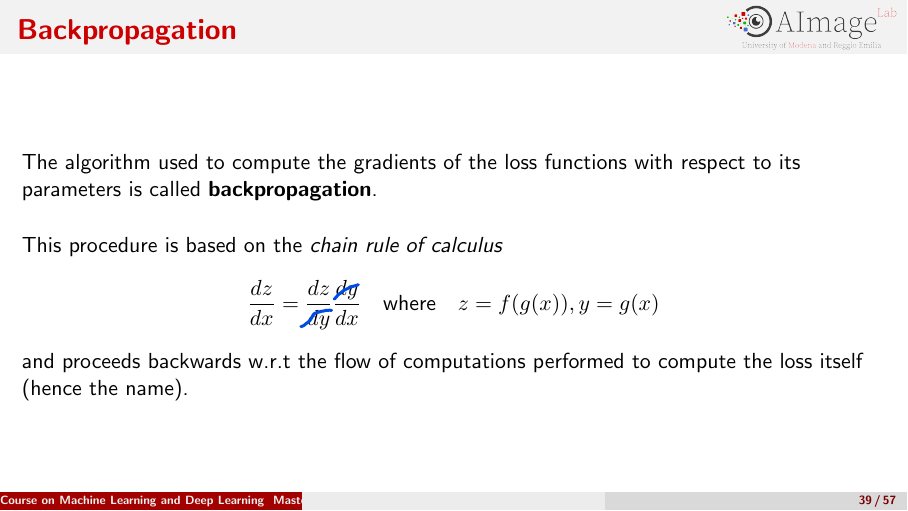
\includegraphics[keepaspectratio]{figure/fig_e1f0f82c6f896cd9.png}}
\caption{Slide 39 -- Regola della catena, con annotazioni}
\end{figure}
% END F01-B0274

% BEGIN F01-B0275
\textbf{Esempio:} \(z = (3x+1)^2\).
% END F01-B0275

% BEGIN F01-B0276
\begin{enumerate}
\def\labelenumi{\arabic{enumi}.}
\tightlist
\item
  Si pone \(y = 3x+1\), quindi \(z = y^2\).
\item
  \(\dfrac{dz}{dy} = 2y\) e \(\dfrac{dy}{dx} = 3\).
\item
  \(\dfrac{dz}{dx} = 2y\cdot 3 = 6(3x+1)\).
\end{enumerate}
% END F01-B0276

% BEGIN F01-B0277
La procedura procede \textbf{all\textquotesingle indietro} rispetto al flusso di calcoli fatto per ottenere la loss, da qui il nome.
% END F01-B0277

% BEGIN F01-B0278
\subsection{Le due derivate locali di uno strato (slide 40)}\label{f01-r751}
% END F01-B0278

% BEGIN F01-B0279
La backpropagation è un processo \textbf{locale}: un neurone (o uno strato) non conosce la topologia della rete in cui si trova. Perché l\textquotesingle algoritmo funzioni, ogni strato deve saper calcolare \textbf{solo due cose}.
% END F01-B0279

% BEGIN F01-B0280
Si consideri lo strato \(i\), con ingresso \(h_i\in\mathbb{R}^d\), parametri \(W_{i+1}\in\mathbb{R}^{k\times d}\) (\(k\) righe = uscite, \(d\) colonne = ingressi) e uscita \(h_{i+1}\in\mathbb{R}^k\). Con attivazione ReLU (bias incorporato in \(W\)):
% END F01-B0280

% BEGIN F01-B0281
\begin{center}
\begin{adjustbox}{max width=\linewidth}
$\displaystyle 
h_{i+1} = \max\big(0,\; W_{i+1}h_i\big)
$
\end{adjustbox}
\end{center}
% END F01-B0281

% BEGIN F01-B0282
\begin{figure}[H]
\centering
\pandocbounded{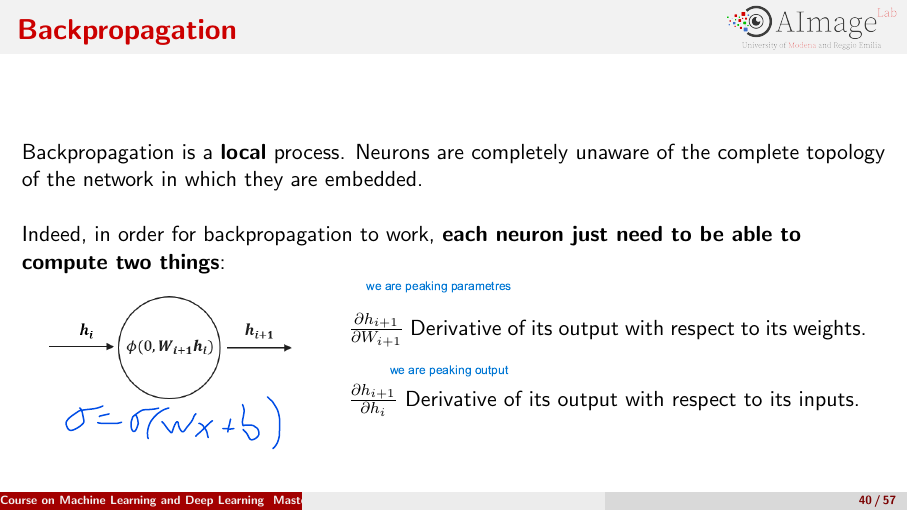
\includegraphics[keepaspectratio]{figure/fig_148b8cd02522274b.png}}
\caption{Slide 40 -- Le due derivate locali, con annotazioni}
\end{figure}
% END F01-B0282

% BEGIN F01-B0283
Le due derivate da saper calcolare sono:
% END F01-B0283

% BEGIN F01-B0284
\begin{enumerate}
\def\labelenumi{\arabic{enumi}.}
\tightlist
\item
  \textbf{la derivata dell\textquotesingle uscita rispetto ai pesi}, \(\dfrac{\partial h_{i+1}}{\partial W_{i+1}}\), che serve ad \textbf{aggiornare} i pesi dello strato;
\item
  \textbf{la derivata dell\textquotesingle uscita rispetto all\textquotesingle ingresso}, \(\dfrac{\partial h_{i+1}}{\partial h_i}\), che serve a \textbf{passare il gradiente} allo strato precedente.
\end{enumerate}
% END F01-B0284

% BEGIN F01-B0285
\textbf{Calcolo nel caso scalare.} Un neurone con un ingresso: \(h_{i+1} = \max(0,\; w\,h_i)\). Si considera il caso "acceso" (\(w h_i > 0\)), in cui la ReLU è l\textquotesingle identità e lo strato è lineare, \(h_{i+1} = w\,h_i\). Come per \(a\cdot x\), la cui derivata rispetto a \(x\) è \(a\):
% END F01-B0285

% BEGIN F01-B0286
\begin{itemize}
\tightlist
\item
  \(\dfrac{\partial h_{i+1}}{\partial w} = h_i\): la derivata rispetto al peso \textbf{"preleva" l\textquotesingle ingresso};
\item
  \(\dfrac{\partial h_{i+1}}{\partial h_i} = w\): la derivata rispetto all\textquotesingle ingresso \textbf{"preleva" il peso}.
\end{itemize}
% END F01-B0286

% BEGIN F01-B0287
Se il neurone è spento (\(w h_i < 0\)), l\textquotesingle uscita è costantemente 0 ed entrambe le derivate valgono \textbf{0}.
% END F01-B0287

% BEGIN F01-B0288
\textbf{Calcolo nel caso vettoriale, passo passo.} Si chiama \(z = W_{i+1}h_i\) (il "pre-attivazione", \(k\) componenti).
% END F01-B0288

% BEGIN F01-B0289
\begin{enumerate}
\def\labelenumi{\arabic{enumi}.}
\tightlist
\item
  La componente \(k\) è \(z_k = \sum_{j=1}^{d} W_{kj}\,h_{i,j}\), quindi \(\dfrac{\partial z_k}{\partial W_{kj}} = h_{i,j}\) e \(\dfrac{\partial z_k}{\partial h_{i,j}} = W_{kj}\).
\item
  La ReLU agisce componente per componente: \(h_{i+1,k} = \max(0, z_k)\), con derivata \(m_k = \mathbb{1}[z_k > 0]\) (1 se il neurone è acceso, 0 se spento).
\item
  Per la catena: \(\dfrac{\partial h_{i+1,k}}{\partial W_{kj}} = m_k\,h_{i,j}\) e \(\dfrac{\partial h_{i+1,k}}{\partial h_{i,j}} = m_k\,W_{kj}\).
\item
  Nella backpropagation arriva da valle il vettore \(g = \partial\mathcal{L}/\partial h_{i+1}\) (\(k\) componenti). Si calcola prima \(\delta = g \odot m\), cioè si azzera il gradiente dei neuroni spenti. Allora: \begin{center}
\begin{adjustbox}{max width=\linewidth}
$\displaystyle \boxed{\frac{\partial\mathcal{L}}{\partial W_{i+1}} = \delta\, h_i^{T} \in \mathbb{R}^{k\times d}}\qquad\boxed{\frac{\partial\mathcal{L}}{\partial h_i} = W_{i+1}^{T}\,\delta \in \mathbb{R}^{d}}$
\end{adjustbox}
\end{center}
\end{enumerate}
% END F01-B0289

% BEGIN F01-B0290
Le forme tornano: il gradiente rispetto a \(W\) ha la stessa forma di \(W\) (\(k\times d\)), quello rispetto a \(h_i\) la stessa forma di \(h_i\) (\(d\)). Le due formule sono la versione matriciale di "preleva l\textquotesingle ingresso" (\(h_i^T\)) e "preleva il peso" (\(W^T\)).
% END F01-B0290

% BEGIN F01-B0291
\begin{quote}
\textbf{Derivate locali e addestramento}
\end{quote}
% END F01-B0291

% BEGIN F01-B0292
\begin{quote}
Per propagare il gradiente bastano le derivate locali necessarie alla regola della catena, calcolate esplicitamente o mediante differenziazione automatica. Ai punti non differenziabili occorre una convenzione appropriata. Questo rende calcolabile il backward, ma non garantisce convergenza o buona generalizzazione.
\end{quote}
% END F01-B0292

% BEGIN F01-B0293
Con un bias \(b\in\mathbb{R}^k\), \(z=Wh+b\) e \(\partial z_j/\partial b_i=\delta_{ij}\): pertanto \(\boxed{\nabla_b\mathcal L=\delta\in\mathbb{R}^k}\).
% END F01-B0293

% BEGIN F01-B0294
\subsection{Il gradiente che si propaga (slide 41)}\label{f01-r790}
% END F01-B0294

% BEGIN F01-B0295
Durante la backpropagation lo strato riceve da valle \(\dfrac{\partial\mathcal{L}}{\partial h_{i+1}}\), cioè l\textquotesingle influenza della sua uscita sull\textquotesingle uscita dell\textquotesingle intera rete. Questo gradiente viene \textbf{concatenato} con i due gradienti locali:
% END F01-B0295

% BEGIN F01-B0296
\begin{center}
\begin{adjustbox}{max width=\linewidth}
$\displaystyle 
\frac{\partial \mathcal{L}}{\partial W_{i+1}} = \frac{\partial \mathcal{L}}{\partial h_{i+1}}\,\frac{\partial h_{i+1}}{\partial W_{i+1}} \quad(\text{per aggiornare i pesi}), \qquad
\frac{\partial \mathcal{L}}{\partial h_{i}} = \frac{\partial \mathcal{L}}{\partial h_{i+1}}\,\frac{\partial h_{i+1}}{\partial h_{i}} \quad(\text{passato allo strato precedente})
$
\end{adjustbox}
\end{center}
% END F01-B0296

% BEGIN F01-B0297
\begin{figure}[H]
\centering
\pandocbounded{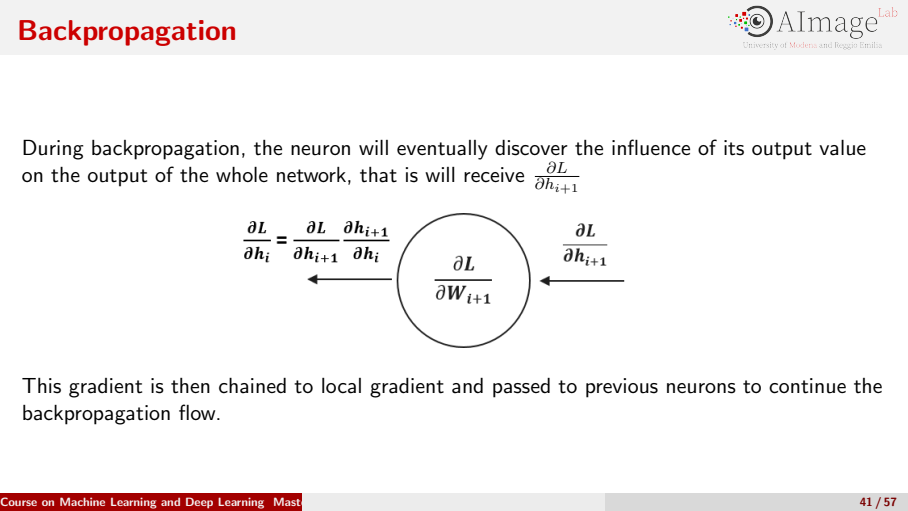
\includegraphics[keepaspectratio]{figure/fig_ebaeb1d2b82ac054.png}}
\caption{Slide 41 -- Concatenazione del gradiente}
\end{figure}
% END F01-B0297

% BEGIN F01-B0298
\subsection{Esempio: MLP a 3 strati con ReLU (slide 42--50)}\label{f01-r801}
% END F01-B0298

% BEGIN F01-B0299
Si consideri un MLP a tre strati, in cui ogni cerchio è uno strato con attivazione ReLU, e un dataset su cui addestrarlo.
% END F01-B0299

% BEGIN F01-B0300
\textbf{1. Forward (slide 43--47).} Si passa un esempio \(x\) attraverso i tre strati e si calcola la penalità della loss sull\textquotesingle uscita:
% END F01-B0300

% BEGIN F01-B0301
\begin{center}
\begin{adjustbox}{max width=\linewidth}
$\displaystyle 
h_1 = \max(0, W_1x),\qquad h_2 = \max(0, W_2h_1),\qquad o = \max(0, W_3h_2),\qquad \mathcal{L} = \text{Loss}(o, y)
$
\end{adjustbox}
\end{center}
% END F01-B0301

% BEGIN F01-B0302
Dato che \(o\) e \(y\) sono numeri, la penalità si calcola con l\textquotesingle equazione della loss scelta. Per applicare la discesa del gradiente servono ora le derivate parziali della loss rispetto a \textbf{ogni} insieme di parametri. Le si calcola \textbf{strato per strato, a partire dall\textquotesingle ultimo}: prima \(W_3\), poi \(W_2\), poi \(W_1\).
% END F01-B0302

% BEGIN F01-B0303
\textbf{2. Gradiente rispetto a \(W_3\) (slide 47--48).} Tra \(\mathcal{L}\) e \(W_3\) non c\textquotesingle è una dipendenza diretta: in mezzo c\textquotesingle è l\textquotesingle equazione della loss (un quadrato, un esponenziale, \ldots), che è a sua volta una funzione di \(o\). Si applica la regola della catena una prima volta:
% END F01-B0303

% BEGIN F01-B0304
\begin{center}
\begin{adjustbox}{max width=\linewidth}
$\displaystyle 
\boxed{\frac{\partial\mathcal{L}}{\partial W_3} = \frac{\partial\mathcal{L}}{\partial o}\cdot\frac{\partial o}{\partial W_3}}
$
\end{adjustbox}
\end{center}
% END F01-B0304

% BEGIN F01-B0305
\begin{itemize}
\tightlist
\item
  \(\dfrac{\partial o}{\partial W_3}\) è la derivata locale di §8.2: vale \(h_2\) se il neurone è acceso, \(0\) se è spento.
\item
  \(\dfrac{\partial\mathcal{L}}{\partial o}\) dipende dall\textquotesingle equazione della loss: ad esempio \(2(o-y)\) per la MSE, oppure \(\text{softmax}(o) - y\) per la cross-entropy (§7.2).
\end{itemize}
% END F01-B0305

% BEGIN F01-B0306
Una volta calcolato il valore numerico (su un esempio, su un batch o su tutto il dataset, come nella discesa del gradiente classica), si prepara l'aggiornamento del parametro. \textbf{Tutti i gradienti si calcolano con gli stessi pesi del forward; gli aggiornamenti si applicano solo dopo avere completato il backward:}
% END F01-B0306

% BEGIN F01-B0307
\begin{center}
\begin{adjustbox}{max width=\linewidth}
$\displaystyle 
W_3^{new} = W_3 - \alpha\,\frac{\partial\mathcal{L}}{\partial W_3}
$
\end{adjustbox}
\end{center}
% END F01-B0307

% BEGIN F01-B0308
\begin{figure}[H]
\centering
\pandocbounded{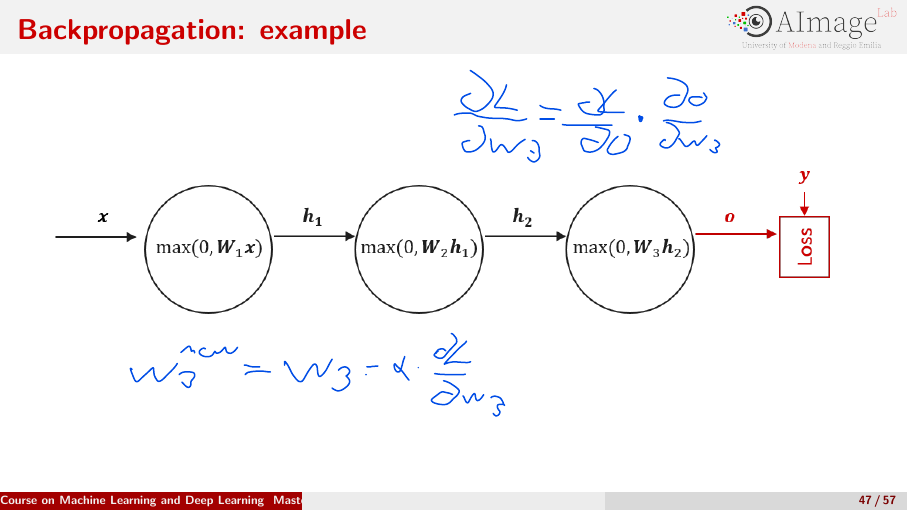
\includegraphics[keepaspectratio]{figure/fig_76b50c6991feb177.png}}
\caption{Slide 47 -- Gradiente e aggiornamento di W3, con annotazioni}
\end{figure}
% END F01-B0308

% BEGIN F01-B0309
\textbf{3. Gradiente rispetto a \(W_2\) (slide 49).} Anche qui non c\textquotesingle è dipendenza diretta, perché tra la loss e \(W_2\) c\textquotesingle è un altro strato.
% END F01-B0309

% BEGIN F01-B0310
Un primo tentativo naturale ma \textbf{sbagliato} è \(\frac{\partial\mathcal{L}}{\partial o}\cdot\frac{\partial o}{\partial W_3}\cdot\frac{\partial W_3}{\partial W_2}\). Non esiste alcuna equazione che leghi \(W_3\) a \(W_2\): sono parametri \textbf{indipendenti}, quindi \(\partial W_3/\partial W_2=0\): quel percorso non esprime la dipendenza della loss da \(W_2\).
% END F01-B0310

% BEGIN F01-B0311
La strada giusta è passare attraverso le \textbf{attivazioni}, che sono legate tra loro dalle equazioni degli strati:
% END F01-B0311

% BEGIN F01-B0312
\begin{itemize}
\tightlist
\item
  \(o\) dipende da \(h_2\) tramite \(o = \max(0, W_3h_2)\);
\item
  \(h_2\) dipende da \(W_2\) tramite \(h_2 = \max(0, W_2h_1)\).
\end{itemize}
% END F01-B0312

% BEGIN F01-B0313
\begin{center}
\begin{adjustbox}{max width=\linewidth}
$\displaystyle 
\boxed{\frac{\partial\mathcal{L}}{\partial W_2} = \frac{\partial\mathcal{L}}{\partial o}\cdot\frac{\partial o}{\partial h_2}\cdot\frac{\partial h_2}{\partial W_2}}
$
\end{adjustbox}
\end{center}
% END F01-B0313

% BEGIN F01-B0314
Per §8.2, nel caso acceso \(\dfrac{\partial o}{\partial h_2} = W_3\) ("preleva il peso") e \(\dfrac{\partial h_2}{\partial W_2} = h_1\) ("preleva l\textquotesingle ingresso"). I primi due fattori insieme sono \(\dfrac{\partial\mathcal{L}}{\partial h_2}\), la freccia rossa che torna indietro nella slide 49.
% END F01-B0314

% BEGIN F01-B0315
\begin{figure}[H]
\centering
\pandocbounded{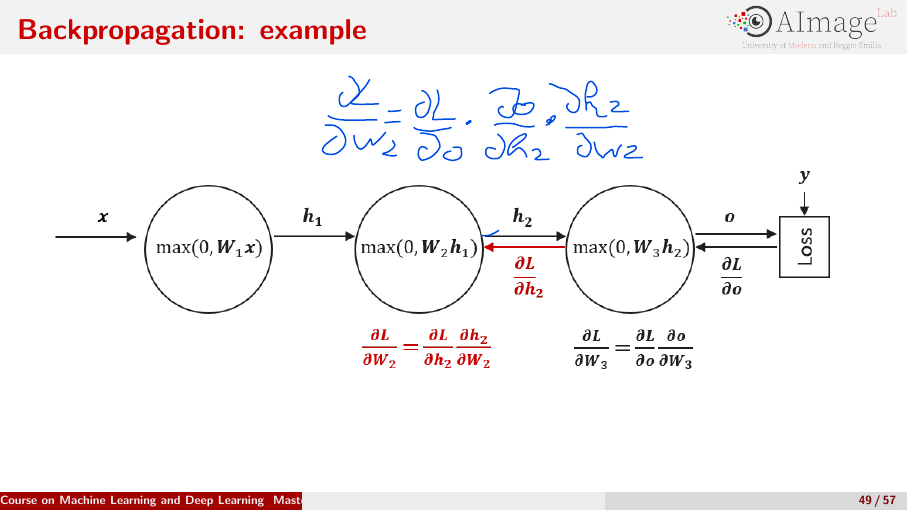
\includegraphics[keepaspectratio]{figure/fig_a1f97259021427be.png}}
\caption{Slide 49 -- Gradiente di W2, con annotazioni}
\end{figure}
% END F01-B0315

% BEGIN F01-B0316
\textbf{4. Gradiente rispetto a \(W_1\) (slide 50).} Stesso ragionamento, con un anello in più nella catena:
% END F01-B0316

% BEGIN F01-B0317
\begin{center}
\begin{adjustbox}{max width=\linewidth}
$\displaystyle 
\boxed{\frac{\partial\mathcal{L}}{\partial W_1} = \frac{\partial\mathcal{L}}{\partial o}\cdot\frac{\partial o}{\partial h_2}\cdot\frac{\partial h_2}{\partial h_1}\cdot\frac{\partial h_1}{\partial W_1}}
$
\end{adjustbox}
\end{center}
% END F01-B0317

% BEGIN F01-B0318
\begin{figure}[H]
\centering
\pandocbounded{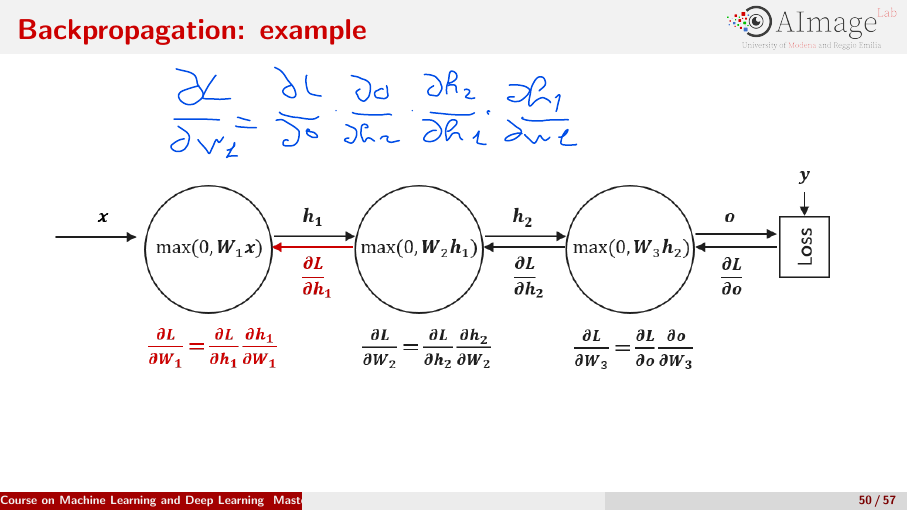
\includegraphics[keepaspectratio]{figure/fig_dabdbb34b5bf3150.png}}
\caption{Slide 50 -- Backpropagation completa, con annotazioni}
\end{figure}
% END F01-B0318

% BEGIN F01-B0319
\textbf{La forma generale.} Per ogni strato, il gradiente dei pesi è sempre \textbf{"gradiente della loss rispetto all\textquotesingle uscita dello strato" × "derivata dell\textquotesingle uscita rispetto ai pesi"}:
% END F01-B0319

% BEGIN F01-B0320
\begin{center}
\begin{adjustbox}{max width=\linewidth}
$\displaystyle 
\frac{\partial\mathcal{L}}{\partial W_3} = \frac{\partial\mathcal{L}}{\partial o}\frac{\partial o}{\partial W_3},\qquad
\frac{\partial\mathcal{L}}{\partial W_2} = \frac{\partial\mathcal{L}}{\partial h_2}\frac{\partial h_2}{\partial W_2},\qquad
\frac{\partial\mathcal{L}}{\partial W_1} = \frac{\partial\mathcal{L}}{\partial h_1}\frac{\partial h_1}{\partial W_1}
$
\end{adjustbox}
\end{center}
% END F01-B0320

% BEGIN F01-B0321
E i gradienti rispetto alle uscite si ottengono uno dall\textquotesingle altro, \textbf{riusando quello appena calcolato}:
% END F01-B0321

% BEGIN F01-B0322
\begin{center}
\begin{adjustbox}{max width=\linewidth}
$\displaystyle 
\frac{\partial\mathcal{L}}{\partial h_2} = \frac{\partial\mathcal{L}}{\partial o}\cdot\frac{\partial o}{\partial h_2},\qquad
\frac{\partial\mathcal{L}}{\partial h_1} = \frac{\partial\mathcal{L}}{\partial h_2}\cdot\frac{\partial h_2}{\partial h_1}
$
\end{adjustbox}
\end{center}
% END F01-B0322

% BEGIN F01-B0323
Per \(W_1\) non si ricalcola tutta la catena da zero: si prende \(\partial\mathcal{L}/\partial h_2\), già calcolato per \(W_2\), e lo si moltiplica per un solo fattore locale. Per questo si procede \textbf{dall\textquotesingle ultimo strato al primo}: ogni strato riceve il gradiente da valle, lo usa e lo passa a monte. È ciò che rende l\textquotesingle algoritmo efficiente.
% END F01-B0323

% BEGIN F01-B0324
\textbf{5. Il ciclo completo.} Aggiornati i parametri, si prende un altro esempio o un altro batch, si ripete forward, backward e aggiornamento, e si itera fino a convergenza: è la discesa del gradiente stocastica.
% END F01-B0324

% BEGIN F01-B0325
\pandocbounded{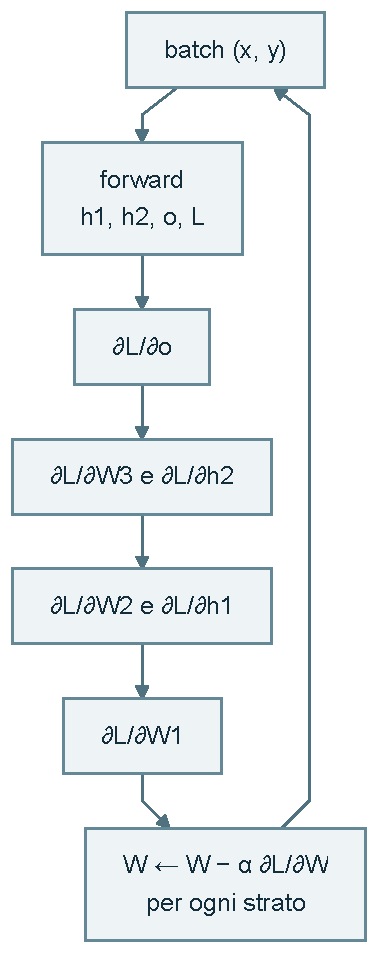
\includegraphics[keepaspectratio]{figure/diagramma_f01_03.pdf}}
% END F01-B0325

% BEGIN F01-B0326
\begin{quote}
\textbf{Esempio numerico (rete scalare, un neurone per strato)}
\end{quote}
% END F01-B0326

% BEGIN F01-B0327
\begin{quote}
Con \(x = 1\), \(y = 2\), \(w_1 = 0.5\), \(w_2 = 2\), \(w_3 = 1.5\), ReLU e loss \(\mathcal{L} = (o-y)^2\).

\textbf{Forward:} - \(h_1 = \max(0,\ 0.5\cdot1) = 0.5\) - \(h_2 = \max(0,\ 2\cdot0.5) = 1\) - \(o = \max(0,\ 1.5\cdot1) = 1.5\) - \(\mathcal{L} = (1.5-2)^2 = 0.25\)

Tutti i neuroni sono accesi, quindi le ReLU si comportano come identità.

\textbf{Backward}, dall\textquotesingle uscita verso l\textquotesingle ingresso:

\begin{longtable}[]{@{}
  >{\raggedright\arraybackslash}p{(\linewidth - 4\tabcolsep) * \real{0.3333}}
  >{\raggedright\arraybackslash}p{(\linewidth - 4\tabcolsep) * \real{0.3333}}
  >{\raggedright\arraybackslash}p{(\linewidth - 4\tabcolsep) * \real{0.3333}}@{}}
\toprule\noalign{}
\begin{minipage}[b]{\linewidth}\raggedright
Passo
\end{minipage} & \begin{minipage}[b]{\linewidth}\raggedright
Formula
\end{minipage} & \begin{minipage}[b]{\linewidth}\raggedright
Valore
\end{minipage} \\
\midrule\noalign{}
\endhead
\bottomrule\noalign{}
\endlastfoot
\(\partial\mathcal{L}/\partial o\) & \(2(o-y)\) & \(2(1.5-2) = -1\) \\
\(\partial\mathcal{L}/\partial w_3\) & \(\partial\mathcal{L}/\partial o \cdot h_2\) & \(-1\cdot1 = -1\) \\
\(\partial\mathcal{L}/\partial h_2\) & \(\partial\mathcal{L}/\partial o \cdot w_3\) & \(-1\cdot1.5 = -1.5\) \\
\(\partial\mathcal{L}/\partial w_2\) & \(\partial\mathcal{L}/\partial h_2 \cdot h_1\) & \(-1.5\cdot0.5 = -0.75\) \\
\(\partial\mathcal{L}/\partial h_1\) & \(\partial\mathcal{L}/\partial h_2 \cdot w_2\) & \(-1.5\cdot2 = -3\) \\
\(\partial\mathcal{L}/\partial w_1\) & \(\partial\mathcal{L}/\partial h_1 \cdot x\) & \(-3\cdot1 = -3\) \\
\end{longtable}

\textbf{Aggiornamento} con \(\alpha = 0.05\): - \(w_1 = 0.5 + 0.15 = 0.65\) - \(w_2 = 2 + 0.0375 = 2.0375\) - \(w_3 = 1.5 + 0.05 = 1.55\)

\textbf{Nuovo forward:} \(o = 2.053\) e \(\mathcal{L} = 0.0028\), molto più vicino al target. I gradienti sono stati verificati numericamente con le differenze finite.
\end{quote}
% END F01-B0327

% BEGIN F01-B0328
\subsection{Perché la backpropagation è così importante}\label{f01-r914}
% END F01-B0328

% BEGIN F01-B0329
\begin{itemize}
\tightlist
\item
  \textbf{Vale per qualunque strato.} Nelle formule di §8.4 non si specifica mai l\textquotesingle equazione degli strati: si scrive solo \(\partial h_2/\partial h_1\) o \(\partial h_1/\partial W_1\). L\textquotesingle algoritmo vale quindi per qualunque strato di cui si sappiano calcolare le due derivate locali, ed è questo che dà la libertà di costruire qualunque architettura.
\item
  \textbf{È lo stesso algoritmo dal 1986.} Ciò che è cambiato è l\textquotesingle{}\textbf{ottimizzatore}, cioè la regola di aggiornamento (SGD, Adam, \ldots), ma il modo di calcolare i gradienti è rimasto identico. In oltre 30 anni nessuno ha trovato un metodo migliore per efficienza, scalabilità e tempo di calcolo; ci sono stati tentativi, alcuni buoni e altri meno.
\item
  \textbf{La usa ogni rete.} Chi ha addestrato una rete, ad esempio per la tesi triennale, l\textquotesingle ha usata senza saperlo, che fosse un Transformer, una rete convoluzionale o altro. In PyTorch è ciò che esegue \texttt{loss.backward()} (vedi 01 Introduzione PyTorch e 02 LogReg torch optim).
\end{itemize}
% END F01-B0329

% BEGIN F01-B0330
\begin{center}\rule{0.5\linewidth}{0.5pt}\end{center}
% END F01-B0330

% BEGIN F01-B0331
\section{Inizializzazione dei pesi (slide 51)}\label{f01-r922}
% END F01-B0331

% BEGIN F01-B0332
La discesa del gradiente parte da una \textbf{inizializzazione casuale} dei pesi. Con 10 o 20 pesi la cosa sembra banale; con milioni, miliardi o migliaia di miliardi di pesi anche l\textquotesingle inizializzazione diventa un problema. I requisiti sono due.
% END F01-B0332

% BEGIN F01-B0333
\textbf{1. Pesi piccoli, per evitare l\textquotesingle esplosione dei valori.} Si consideri uno strato con \(n = 10\,000\) ingressi. Ogni neurone calcola una somma di 10 000 termini \(w_j x_j\).
% END F01-B0333

% BEGIN F01-B0334
\begin{itemize}
\tightlist
\item
  Se tutti i pesi valessero 1 e gli ingressi fossero circa 100, l\textquotesingle uscita sarebbe circa \(10\,000\cdot100 = 10^6\).
\item
  Strato dopo strato, numeri così crescono senza controllo.
\end{itemize}
% END F01-B0334

% BEGIN F01-B0335
Si vuole quindi evitare il più possibile che la grandezza delle uscite degli strati cresca, e per questo all\textquotesingle inizio servono pesi \textbf{molto piccoli}, ma non trascurabili.
% END F01-B0335

% BEGIN F01-B0336
\textbf{2. Pesi diversi tra loro, per rompere la simmetria.} I pesi non possono essere tutti uguali. Se neuroni permutabili sono inizializzati simmetricamente sia nelle connessioni entranti sia in quelle uscenti, ricevono gli stessi aggiornamenti:
% END F01-B0336

% BEGIN F01-B0337
\begin{enumerate}
\def\labelenumi{\arabic{enumi}.}
\tightlist
\item
  con le stesse righe in \(W\), tutti i neuroni calcolano la \textbf{stessa uscita};
\item
  ricevono quindi lo \textbf{stesso gradiente} (\(\delta h^T\) ha righe uguali);
\item
  subiscono lo \textbf{stesso aggiornamento};
\item
  restano uguali per sempre, e lo strato si comporta come un solo neurone.
\end{enumerate}
% END F01-B0337

% BEGIN F01-B0338
Ogni neurone riesce a imparare qualcosa di diverso solo perché parte da pesi diversi.
% END F01-B0338

% BEGIN F01-B0339
\textbf{La prassi} è campionare valori \textbf{piccoli, attorno allo zero, positivi o negativi}, ad esempio da una gaussiana a media zero, e mettere i \textbf{bias a zero}. Il difficile è trovare per ogni neurone pesi abbastanza piccoli da evitare problemi numerici e, allo stesso tempo, abbastanza diversi da quelli degli altri neuroni dello strato.
% END F01-B0339

% BEGIN F01-B0340
\textbf{Scalare con il fan-in (inizializzazione di Glorot).} Un trucco molto diffuso è \textbf{scalare i pesi in base al fan-in} del neurone, cioè al numero dei suoi ingressi. Per controllare la varianza della somma, la deviazione standard dei pesi si scala in proporzione a \(1/\sqrt{n}\); dividere i pesi per \(n\) ridurrebbe eccessivamente la varianza, come mostra il calcolo seguente.
% END F01-B0340

% BEGIN F01-B0341
\textbf{Perché funziona, passo passo.} Si calcola la varianza dell\textquotesingle uscita \(z = \sum_{j=1}^{n} w_j x_j\) di un neurone con \(n\) ingressi.
% END F01-B0341

% BEGIN F01-B0342
\begin{enumerate}
\def\labelenumi{\arabic{enumi}.}
\tightlist
\item
  Si assume che i pesi \(w_j\) siano indipendenti, a media zero, con varianza \(\sigma_w^2\), e per semplicità ingressi fissati con \(x_j^2 = 1\).
\item
  La varianza di una somma di termini indipendenti è la somma delle varianze: \(\text{Var}(z) = \sum_j \text{Var}(w_j x_j)\).
\item
  Ogni termine vale \(\text{Var}(w_j x_j) = x_j^2\,\sigma_w^2 = \sigma_w^2\).
\item
  Quindi \(\text{Var}(z) = n\,\sigma_w^2\): la deviazione standard dell\textquotesingle uscita è \(\sqrt{n}\,\sigma_w\) e \textbf{cresce con il numero di ingressi}.
\item
  Per mantenerla dell\textquotesingle ordine di 1 serve \(\sigma_w^2 = 1/n\), cioè pesi con deviazione standard \(1/\sqrt{n}\).
\end{enumerate}
% END F01-B0342

% BEGIN F01-B0343
\begin{longtable}[]{@{}ll@{}}
\toprule\noalign{}
Pesi (\(n = 10\,000\), \(x_j = 1\)) & Deviazione standard di \(z\) \\
\midrule\noalign{}
\endhead
\bottomrule\noalign{}
\endlastfoot
\(\mathcal{N}(0, 1)\) & \(\approx 100\) \\
\(\mathcal{N}(0, 1/n)\), cioè std \(1/\sqrt{n}\) & \(\approx 1\) \\
\(\mathcal{N}(0,1)/n\) & \(\approx 0.01\) (troppo piccola) \\
\end{longtable}
% END F01-B0343

% BEGIN F01-B0344
\begin{quote}
\textbf{Precisazione sulle formule esatte}
\end{quote}
% END F01-B0344

% BEGIN F01-B0345
\begin{quote}
Dividere per \(n\) dà l\textquotesingle idea, ma per tenere la varianza costante si scala la \textbf{varianza} per \(1/\text{fan-in}\), cioè la deviazione standard per \(1/\sqrt{\text{fan-in}}\). Le varianti note sono: - \textbf{Glorot/Xavier}: \(\text{Var}(w) = 2/(\text{fan-in} + \text{fan-out})\); - \textbf{He}: \(2/\text{fan-in}\), pensata per la ReLU.
\end{quote}
% END F01-B0345

% BEGIN F01-B0346
Tutte queste strategie sono già implementate in \textbf{PyTorch}, non vanno scritte a mano. Quando si crea uno strato lineare (\texttt{nn.Linear}), è già inizializzato; si può scegliere un\textquotesingle altra inizializzazione (gaussiana, uniforme, Glorot, \ldots) con le funzioni di \texttt{torch.nn.init}.
% END F01-B0346

% BEGIN F01-B0347
\begin{center}\rule{0.5\linewidth}{0.5pt}\end{center}
% END F01-B0347

% BEGIN F01-B0348
\section{Regolarizzazione nelle reti profonde (slide 52--56)}\label{f01-r969}
% END F01-B0348

% BEGIN F01-B0349
\subsection{Regolarizzazione implicita (slide 53)}\label{f01-r971}
% END F01-B0349

% BEGIN F01-B0350
Le reti profonde hanno una \textbf{capacità rappresentazionale molto alta}: è un bene, perché possono apprendere funzioni complesse. Per lo stesso motivo, però, sono soggette a overfitting se non vengono regolarizzate.
% END F01-B0350

% BEGIN F01-B0351
\begin{itemize}
\tightlist
\item
  È facilissimo aggiungere milioni di parametri, mentre il dataset contiene magari migliaia di esempi: quasi sempre ci sono più parametri che dati.
\item
  Oltre ai \textbf{regolarizzatori espliciti} (\(L_1\), \(L_2\) di §7.4), che sono scritti nella loss e agiscono tramite i gradienti, esistono tecniche \textbf{implicite}.
\item
  Si chiamano implicite perché non compaiono nell\textquotesingle equazione da ottimizzare: sono \textbf{accorgimenti applicati durante l\textquotesingle apprendimento} che costringono la rete a regolarizzarsi.
\end{itemize}
% END F01-B0351

% BEGIN F01-B0352
\subsection{Dropout (slide 54)}\label{f01-r979}
% END F01-B0352

% BEGIN F01-B0353
\begin{figure}[H]
\centering
\pandocbounded{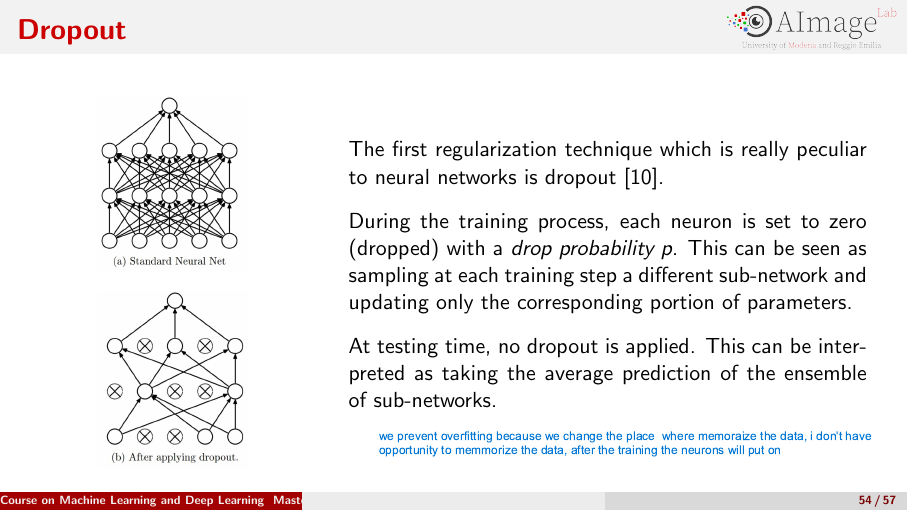
\includegraphics[keepaspectratio]{figure/fig_50efc11447727fca.png}}
\caption{Slide 54 -- Dropout, con annotazioni}
\end{figure}
% END F01-B0353

% BEGIN F01-B0354
Il \textbf{dropout} è la tecnica implicita più popolare. Ha come iperparametro una \textbf{probabilità di drop \(p\) per ogni strato}, tipicamente tra il 10\% e il 50\%.
% END F01-B0354

% BEGIN F01-B0355
\textbf{Come funziona in training:}
% END F01-B0355

% BEGIN F01-B0356
\begin{enumerate}
\def\labelenumi{\arabic{enumi}.}
\tightlist
\item
  per ogni neurone dello strato, prima del forward, si "lancia una moneta" che con probabilità \(p\) dice di spegnerlo;
\item
  il neurone spento ha uscita \textbf{0}, sia nel forward sia nel backward;
\item
  a ogni passo il neurone spento è diverso.
\end{enumerate}
% END F01-B0356

% BEGIN F01-B0357
Formalmente l\textquotesingle uscita dello strato diventa \(\tilde h = r \odot h\), dove ogni \(r_k\) vale 0 con probabilità \(p\) e 1 con probabilità \(1-p\). Nel backward \(\partial\tilde h_k/\partial h_k = r_k\): un neurone spento non riceve gradiente e il suo contributo al gradiente dei pesi in ingresso è nullo in quel passo. Regolarizzazione o memoria dell'ottimizzatore possono comunque modificarli. La maschera campionata nel forward viene mantenuta nel relativo backward.
% END F01-B0357

% BEGIN F01-B0358
Il risultato è che si tagliano \textbf{a caso} alcuni percorsi dentro la rete: la rete non può più usare quei neuroni e deve trovare altre strade. Equivale a \textbf{campionare a ogni passo una sotto-rete diversa} e ad aggiornare solo la sua porzione di parametri.
% END F01-B0358

% BEGIN F01-B0359
\textbf{Perché può ridurre l'overfitting.} Il dropout rende meno affidabile l'uso congiunto di specifiche unità e incoraggia rappresentazioni utili anche quando altre unità mancano. L'immagine dei posti di memoria che cambiano è un'analogia: non dimostra che la memorizzazione diventi impossibile.
% END F01-B0359

% BEGIN F01-B0360
\textbf{In test.} \textbf{Nessun dropout}: dopo il training tutti i neuroni sono attivi. Lo si può interpretare come un'approssimazione della \textbf{predizione di un ensemble} di sotto-reti; per una rete non lineare il riscalamento non è generalmente la loro media esatta.
% END F01-B0360

% BEGIN F01-B0361
\begin{quote}
\textbf{Precisazione: il riscalamento}
\end{quote}
% END F01-B0361

% BEGIN F01-B0362
\begin{quote}
In training ogni neurone è attivo solo con probabilità \(1-p\), quindi in media la sua uscita vale \((1-p)\,h_k\). In test, con tutti i neuroni accesi, varrebbe \(h_k\). Per rendere coerenti le due fasi: - si moltiplicano le uscite per \((1-p)\) in test; - oppure, come fa PyTorch (\emph{inverted dropout}), si dividono per \((1-p)\) in training.
\end{quote}
% END F01-B0362

% BEGIN F01-B0363
\textbf{Perché spegnere neuroni a caso, in modo uniforme.}
% END F01-B0363

% BEGIN F01-B0364
\begin{itemize}
\tightlist
\item
  In training non si sa a priori quali neuroni stiano imparando cosa, e l\textquotesingle addestramento è dinamico: un neurone può imparare una cosa all\textquotesingle inizio e un\textquotesingle altra dopo.
\item
  Si campiona quindi in modo \textbf{uniforme}. Spegnere un neurone che è già spento non cambia nulla: il dropout ha effetto solo sui neuroni effettivamente attivi.
\end{itemize}
% END F01-B0364

% BEGIN F01-B0365
\textbf{Una probabilità per strato.} \(p\) è la stessa per tutti i neuroni di uno strato, ma di solito cambia da strato a strato, in base al numero di neuroni e alla posizione nella rete.
% END F01-B0365

% BEGIN F01-B0366
La probabilità può variare fra strati. Eliminare il 90\% delle unità di uno strato molto stretto può lasciare troppo poca informazione; non esiste una regola generale che vieti la regolarizzazione vicino all'uscita.
% END F01-B0366

% BEGIN F01-B0367
Le probabilità di dropout sono iperparametri da valutare sul validation set. La sensibilità alla loro scelta dipende dal modello e dai dati: non è garantito che le differenze rimangano entro pochi punti percentuali.
% END F01-B0367

% BEGIN F01-B0368
\subsection{Data augmentation (slide 55)}\label{f01-r1015}
% END F01-B0368

% BEGIN F01-B0369
Il modo migliore per generalizzare meglio sarebbe \textbf{allenarsi su più dati}, che però non sempre sono disponibili. La \textbf{data augmentation} genera \textbf{nuovi esempi di training applicando trasformazioni agli input} del training set, trasformazioni che devono \textbf{preservare l\textquotesingle etichetta} dell\textquotesingle esempio originale.
% END F01-B0369

% BEGIN F01-B0370
\begin{figure}[H]
\centering
\pandocbounded{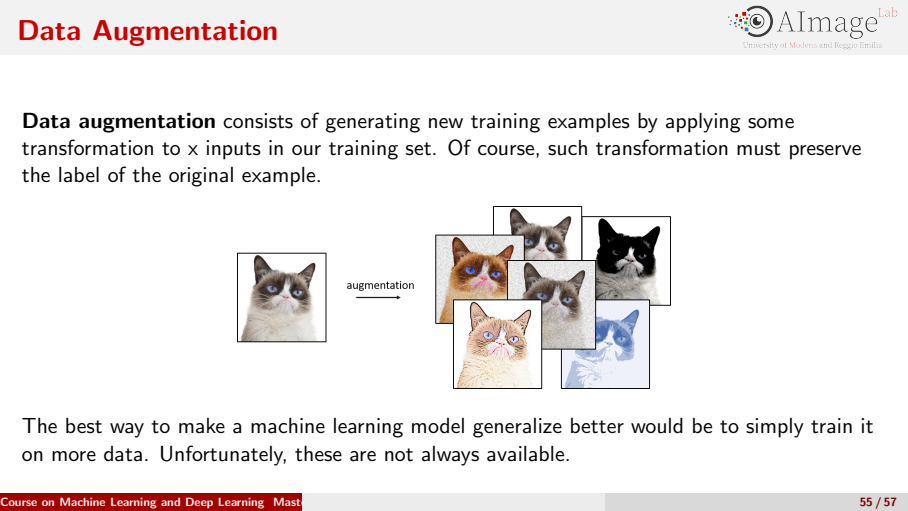
\includegraphics[keepaspectratio]{figure/fig_138dc04a0425d8ee.png}}
\caption{Slide 55 -- Data augmentation}
\end{figure}
% END F01-B0370

% BEGIN F01-B0371
Per un\textquotesingle immagine si applicano trasformazioni \textbf{non distruttive}:
% END F01-B0371

% BEGIN F01-B0372
\begin{itemize}
\tightlist
\item
  una leggera rotazione;
\item
  un cambio di scala;
\item
  un ribaltamento (\emph{flip});
\item
  un cambio di colori, contrasto o luminosità;
\item
  la conversione in bianco e nero.
\end{itemize}
% END F01-B0372

% BEGIN F01-B0373
Si applicano solo le trasformazioni che mantengono valida l'etichetta per il compito scelto.
% END F01-B0373

% BEGIN F01-B0374
\textbf{Due vantaggi contro l\textquotesingle overfitting:}
% END F01-B0374

% BEGIN F01-B0375
\begin{enumerate}
\def\labelenumi{\arabic{enumi}.}
\tightlist
\item
  \textbf{Più dati senza nuove annotazioni.} Con 10 trasformazioni per esempio il dataset diventa 10 volte più grande, e più il dataset è grande, più è difficile memorizzarlo.
\item
  \textbf{Memorizzare diventa inefficiente.} Si creano varianti dello stesso input che devono dare \textbf{la stessa uscita}. Memorizzando, la rete dovrebbe imparare a parte ogni variante: un lavoro moltiplicato per il numero di augmentation. Le conviene invece imparare la \textbf{regola} che porta tutte le varianti alla stessa risposta. In un certo senso si "inganna" la rete, presentandole un problema in cui generalizzare costa meno che memorizzare.
\end{enumerate}
% END F01-B0375

% BEGIN F01-B0376
La data augmentation aumenta la varietà delle osservazioni disponibili e può limitare la memorizzazione. Ogni trasformazione deve conservare il significato del target: una rotazione adatta a una categoria di immagini può cambiare l'etichetta in un altro compito.
% END F01-B0376

% BEGIN F01-B0377
\textbf{Non sempre è facile.} Per le immagini esiste un ampio insieme di trasformazioni non distruttive; per altri dati no.
% END F01-B0377

% BEGIN F01-B0378
\begin{itemize}
\tightlist
\item
  \textbf{Testo.} Una frase non si può ribaltare, ricolorare o ruotare. Servono trasformazioni lessicali, come i sinonimi, che sono più complicate.
\item
  \textbf{Serie temporali} (temperatura, pressione\ldots). Ribaltarle inverte il trend e distrugge l\textquotesingle informazione.
\end{itemize}
% END F01-B0378

% BEGIN F01-B0379
\subsection{Early stopping (slide 56)}\label{f01-r1043}
% END F01-B0379

% BEGIN F01-B0380
Prolungare il training può peggiorare la generalizzazione: l'early stopping usa la validazione per riconoscere quando ulteriori aggiornamenti non migliorano il risultato.
% END F01-B0380

% BEGIN F01-B0381
\textbf{Come si riconosce.} Dopo ogni \textbf{epoca} (un passaggio completo sul dataset) si calcolano due loss:
% END F01-B0381

% BEGIN F01-B0382
\begin{itemize}
\tightlist
\item
  quella sul \textbf{training set}, per vedere se gli aggiornamenti la fanno scendere;
\item
  quella su un piccolo \textbf{validation set}, non usato per l\textquotesingle addestramento.
\end{itemize}
% END F01-B0382

% BEGIN F01-B0383
Se la loss di training continua a scendere mentre quella di validazione \textbf{inizia a salire}, la rete sta entrando nella fase di \textbf{memorizzazione}: sui dati nuovi comincerà a funzionare peggio.
% END F01-B0383

% BEGIN F01-B0384
\begin{figure}[H]
\centering
\pandocbounded{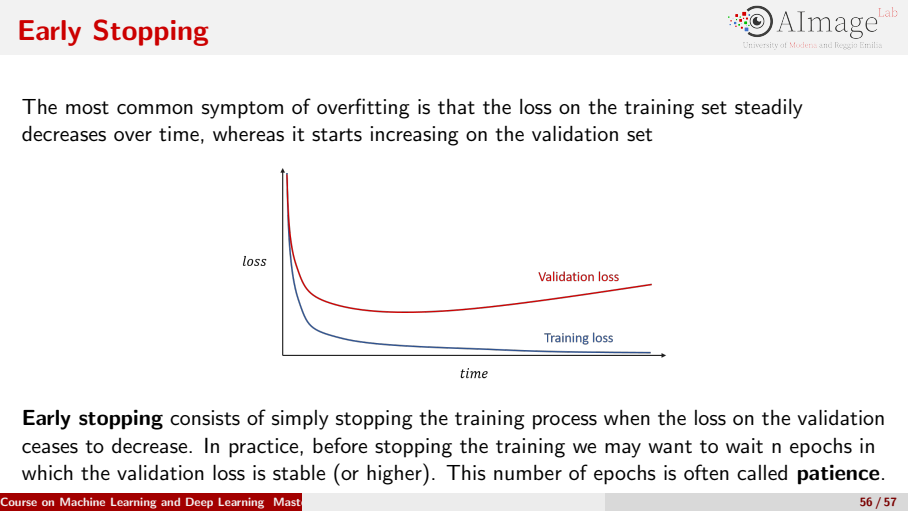
\includegraphics[keepaspectratio]{figure/fig_7187db7a023ba7ac.png}}
\caption{Slide 56 -- Training vs validation loss}
\end{figure}
% END F01-B0384

% BEGIN F01-B0385
\textbf{Early stopping:} si interrompe l'addestramento secondo il criterio di pazienza e si recupera il checkpoint con la migliore metrica di validazione, che può precedere l'ultima epoca. Il test set resta escluso da questa scelta.
% END F01-B0385

% BEGIN F01-B0386
\textbf{La patience.} Non si decide in base a una sola misura, che potrebbe essere una fluttuazione. Si fissa un numero \(n\) di valutazioni consecutive in cui la loss di validazione resta stabile o peggiora prima di fermarsi. Questo numero si chiama \textbf{patience}.
% END F01-B0386

% BEGIN F01-B0387
\begin{center}\rule{0.5\linewidth}{0.5pt}\end{center}
% END F01-B0387

% BEGIN F01-B0388
\section{Riepilogo}\label{f01-r1062}
% END F01-B0388

% BEGIN F01-B0389
\begin{enumerate}
\def\labelenumi{\arabic{enumi}.}
\tightlist
\item
  Il deep learning funziona oggi grazie a \textbf{dati + GPU} e perché \textbf{impara le feature} invece di fissarle. Il prezzo è la loro \textbf{non interpretabilità}.
\item
  \textbf{Classificatore lineare} \(Wx+b\) + \textbf{softmax} + \textbf{cross-entropy} + discesa del gradiente = \textbf{regressione logistica}. La softmax definisce probabilità del modello, senza garantirne la calibrazione.
\item
  \textbf{Neurone artificiale} = mappa affine seguita da un'attivazione; il caso sigmoide corrisponde al modello logistico binario.

  \begin{itemize}
  \tightlist
  \item
    La sigmoide satura (\(\sigma' = \sigma(1-\sigma) \le 0.25\)) e non è centrata.
  \item
    La tanh (\(= 2\sigma(2x)-1\)) è centrata ma satura.
  \item
    La \textbf{ReLU} non satura per \(x>0\) ed è economica.
  \end{itemize}
\item
  \textbf{Senza non linearità} qualunque rete collassa in un singolo strato lineare (\(W = W_2W_1\)).
\item
  \textbf{MLP}: strati fully connected, \(W \in \mathbb{R}^{\text{out}\times\text{in}}\), e \textbf{ogni neurone ha un bias} (6-4-3-1 → 47 parametri). La \textbf{forward propagation} è una composizione di funzioni: la rete è un\textquotesingle equazione esplicita.
\item
  \textbf{Approssimazione universale}: in teoria basta un hidden layer per qualunque funzione continua; in pratica, per la discretizzazione, reti più grandi e profonde sono più espressive. Rappresentare non significa saper imparare.
\item
  \textbf{Funzione obiettivo} \(= \frac1N\sum_i L_i + \lambda\Omega(\theta)\).

  \begin{itemize}
  \tightlist
  \item
    \textbf{Loss:} hinge (margine 1, assorbibile nella scala dei pesi), softmax/cross-entropy (gradiente \(= \text{softmax} - \text{one-hot}\)), MSE.
  \item
    \textbf{Regolarizzatori:} \(L_2\) (pesi piccoli, \emph{weight decay}) e \(L_1\) (pesi nulli).
  \end{itemize}
\item
  \textbf{Backpropagation}:

  \begin{itemize}
  \tightlist
  \item
    regola della catena applicata \textbf{dall\textquotesingle uscita verso l\textquotesingle ingresso};
  \item
    ogni strato calcola solo \(\partial h_{i+1}/\partial W_{i+1}\) ("preleva l\textquotesingle ingresso") e \(\partial h_{i+1}/\partial h_i\) ("preleva il peso");
  \item
    il gradiente rispetto alle attivazioni viene \textbf{riusato} strato dopo strato;
  \item
    funziona per qualunque strato di cui si sappiano scrivere le due derivate ed è invariata dal 1986.
  \end{itemize}
\item
  \textbf{Inizializzazione}: pesi piccoli, a media zero e \textbf{diversi} (rottura della simmetria), scalati con il fan-in; bias a zero.
\item
  \textbf{Regolarizzazione implicita}:

  \begin{itemize}
  \tightlist
  \item
    \textbf{dropout}: spegne neuroni a caso in training, mai in test;
  \item
    \textbf{data augmentation}: varianti con la stessa etichetta;
  \item
    \textbf{early stopping}: si ferma quando la loss di validazione sale, con una \emph{patience}.
  \end{itemize}
\end{enumerate}
% END F01-B0389

% BEGIN F01-B0390
\begin{quote}
\textbf{Riepilogo errata delle slide}
\end{quote}
% END F01-B0390

% BEGIN F01-B0391
\begin{quote}
\begin{itemize}
\tightlist
\item
  \textbf{Slide 15}: \(s_{ship} = 60.75\), non 61.95 (manca il bias).
\item
  \textbf{Slide 18}: denominatore della softmax \(\sum_k e^{z_k}\).
\item
  \textbf{Slide 19}: manca il segno meno nella cross-entropy.
\item
  \textbf{Slide 25}: \(\tanh(x) = 2\sigma(2x) - 1\).
\item
  \textbf{Slide 30}: \(W_2 \in \mathbb{R}^{3\times4}\), \(W_3 \in \mathbb{R}^{1\times3}\).
\end{itemize}
\end{quote}
% END F01-B0391


% BEGIN F02-B0001
\chapter{CNN - Reti neurali convoluzionali}\label{fonte02}
% END F02-B0001

% BEGIN F02-B0002
\begin{indiceargomento}
\item \hyperref[f02-r47]{Rappresentazione Digitale delle Immagini nel Calcolatore (slide 3--6)}
\item \hyperref[f02-r110]{Paradigmi di Computer Vision ed Evoluzione Storica (slide 7--11)}
\item \hyperref[f02-r157]{Limiti del Multilayer Perceptron per Dati Visivi (slide 12--18)}
\item \hyperref[f02-r232]{Principi Architetturali e Ispirazione Biologica (slide 19--23)}
\item \hyperref[f02-r269]{Operatori su Immagini e Sistemi Lineari Traslazione-Invarianti (LSI) (slide 24--34)}
\item \hyperref[f02-r388]{Il Nucleo della Convoluzione nel Deep Learning (slide 35--39)}
\item \hyperref[f02-r483]{Convoluzione Multicanale e Feature Maps (slide 40--42)}
\item \hyperref[f02-r541]{Iperparametri del Livello Convoluzionale: Kernel, Stride e Padding (slide 43--46)}
\item \hyperref[f02-r618]{Calcolo dei Parametri Apprendibili (slide 47)}
\item \hyperref[f02-r657]{Visualizzazione dei Filtri e Gerarchia delle Rappresentazioni (slide 48--51)}
\item \hyperref[f02-r711]{Funzioni di Attivazione e Superamento della ReLU Standard (slide 52--54)}
\item \hyperref[f02-r802]{Livelli di pooling: aggregazione locale e riduzione spaziale (slide 55--58)}
\item \hyperref[f02-r891]{Dalle feature al classificatore: pooling adattivo (slide 59)}
\item \hyperref[f02-r941]{LeNet e AlexNet: evoluzione delle CNN (slide 60--62)}
\item \hyperref[f02-r974]{VGG: distribuire la capacità lungo la profondità (slide 63--68)}
\item \hyperref[f02-r1063]{Profondità e residual learning: ResNet (slide 69--75)}
\item \hyperref[f02-r1134]{Batch Normalization: statistiche e trasformazione appresa (slide 76--86)}
\item \hyperref[f02-r1273]{Riepilogo Formule Operative}
\item \hyperref[f02-r1299]{Errata e precisazioni principali}
\end{indiceargomento}
% END F02-B0002

% BEGIN F02-B0003
\pandocbounded{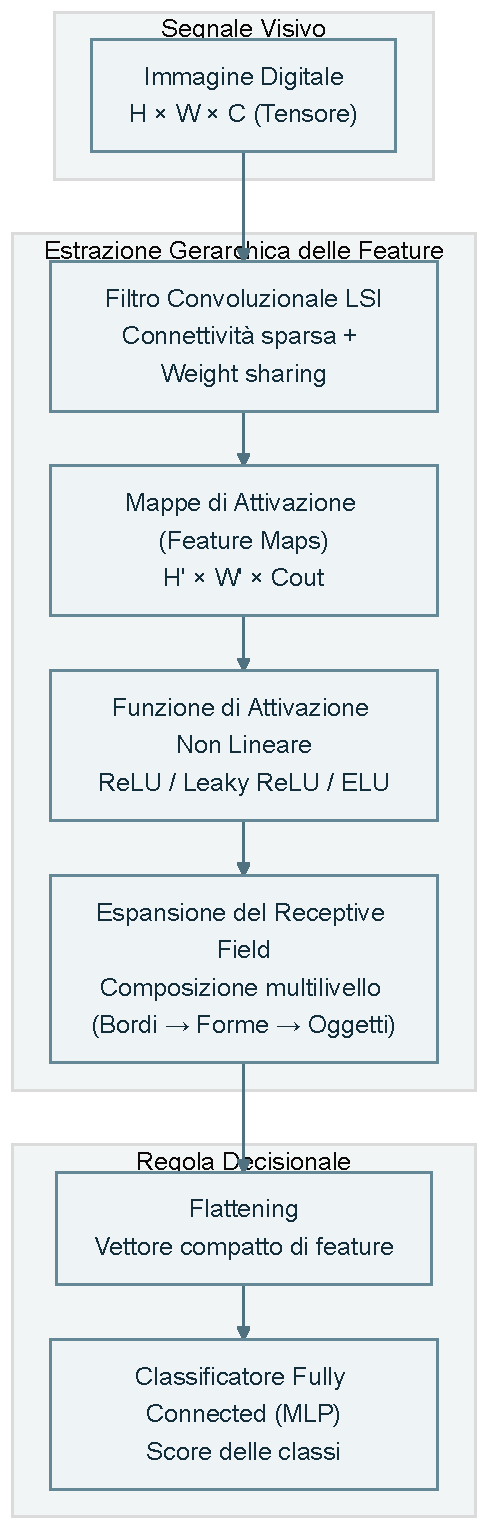
\includegraphics[keepaspectratio]{figure/diagramma_f02_01.pdf}}
% END F02-B0003

% BEGIN F02-B0004
\begin{center}\rule{0.5\linewidth}{0.5pt}\end{center}
% END F02-B0004

% BEGIN F02-B0005
\section{Rappresentazione Digitale delle Immagini nel Calcolatore (slide 3--6)}\label{f02-r47}
% END F02-B0005

% BEGIN F02-B0006
Un\textquotesingle immagine reale è la manifestazione visibile di un fenomeno fisico continuo: la luce riflessa dagli elementi di una scena tridimensionale attraversa il sistema ottico di una fotocamera e incide su una superficie fotosensibile bidimensionale. Il calcolatore, tuttavia, è un dispositivo discreto sia nello spazio sia nei valori numerici che può memorizzare. Il passaggio da un segnale ottico continuo alla sua rappresentazione binaria interna esige pertanto due trasformazioni fondamentali, formalizzate nella Slide 4:
% END F02-B0006

% BEGIN F02-B0007
\begin{enumerate}
\def\labelenumi{\arabic{enumi}.}
\tightlist
\item
  \textbf{Campionamento spaziale (Sampling)}: la scena continua viene discretizzata spazialmente proiettandola su una griglia bidimensionale uniforme composta da \(H \times W\) campioni discreti chiamati \textbf{pixel} (\emph{picture elements}), dove \(H\) denota l\textquotesingle altezza (numero di righe) e \(W\) la larghezza (numero di colonne).
\item
  \textbf{Quantizzazione (Quantization)}: l\textquotesingle intensità luminosa continua misurata da ciascun fotosensore in corrispondenza del singolo pixel viene approssimata e mappata su un insieme discreto di \(2^m\) livelli numerici, corrispondenti a una codifica su \(m\) bit per campione.
\end{enumerate}
% END F02-B0007

% BEGIN F02-B0008
Nella quasi totalità delle applicazioni digitali standard si adotta una profondità di quantizzazione pari a \(m = 8\) bit per canale. Lo spazio dei valori discreti associabili a ogni campione comprende dunque \(2^8 = 256\) intensità distinte, convenzionalmente indicizzate nell\textquotesingle intervallo chiuso:
% END F02-B0008

% BEGIN F02-B0009
\begin{center}
\begin{adjustbox}{max width=\linewidth}
$\displaystyle 
\mathcal{I} \in \{0, 1, 2, \dots, 255\}
$
\end{adjustbox}
\end{center}
% END F02-B0009

% BEGIN F02-B0010
dove il valore \(0\) corrisponde all\textquotesingle assenza totale di segnale luminoso (nero assoluto) e il valore \(255\) corrisponde alla massima intensità di saturazione del sensore (bianco assoluto).
% END F02-B0010

% BEGIN F02-B0011
\begin{figure}[H]
\centering
\pandocbounded{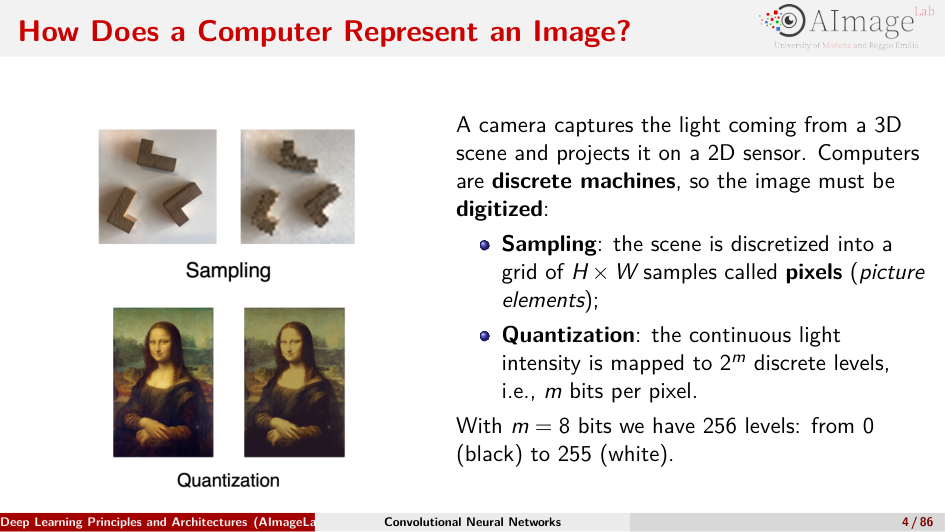
\includegraphics[keepaspectratio]{figure/fig_88296c28495d02db.png}}
\caption{Slide 4 -- How Does a Computer Represent an Image?}
\end{figure}
% END F02-B0011

% BEGIN F02-B0012
\subsection{Immagini in Scala di Grigi (Grayscale)}\label{f02-r64}
% END F02-B0012

% BEGIN F02-B0013
Nel caso di un\textquotesingle immagine monocromatica (in scala di grigi), ciascun pixel memorizza unicamente l\textquotesingle intensità scalare della radianza luminosa. Un\textquotesingle immagine in scala di grigi di risoluzione \(H \times W\) è a tutti gli effetti una matrice numerica:
% END F02-B0013

% BEGIN F02-B0014
\begin{center}
\begin{adjustbox}{max width=\linewidth}
$\displaystyle 
\boxed{I \in \{0, 1, \dots, 255\}^{H \times W}}
$
\end{adjustbox}
\end{center}
% END F02-B0014

% BEGIN F02-B0015
in cui l\textquotesingle elemento \(I(i, j)\) rappresenta il livello di grigio del pixel posizionato alla riga \(i\) (con \(1 \le i \le H\)) e alla colonna \(j\) (con \(1 \le j \le W\)). La Slide 5 illustra questo concetto mostrando una porzione rettangolare (patch) di \(6 \times 8\) pixel estratta da una fotografia di un gatto: ciò che l\textquotesingle occhio umano percepisce come contorni morbidi e sfumature di pelo corrisponde, per la memoria del calcolatore, a una pura tabella bidimensionale di interi compresi tra 0 e 255.
% END F02-B0015

% BEGIN F02-B0016
\begin{figure}[H]
\centering
\pandocbounded{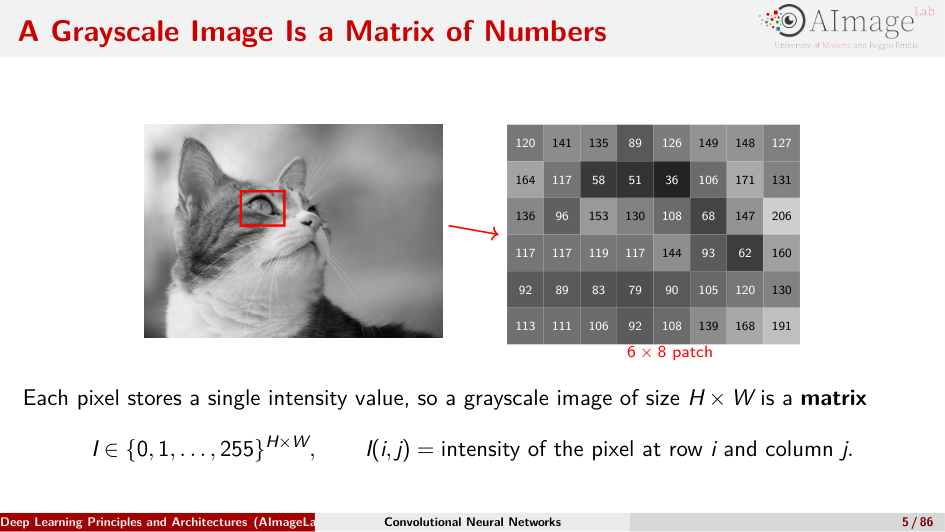
\includegraphics[keepaspectratio]{figure/fig_22f0ae8bd20af6e4.png}}
\caption{Slide 5 -- A Grayscale Image Is a Matrix of Numbers}
\end{figure}
% END F02-B0016

% BEGIN F02-B0017
\subsection{Immagini a Colori: Canali e Spazio RGB}\label{f02-r76}
% END F02-B0017

% BEGIN F02-B0018
La percezione cromatica umana è tricromatica: la retina dispone di tre tipologie distinte di coni fotosensibili, sintonizzati su differenti lunghezze d\textquotesingle onda dello spettro visibile. Nel calcolatore, la sintesi del colore viene implementata attraverso lo spazio \textbf{RGB (Red, Green, Blue)}, basato sul principio della sintesi additiva della luce.
% END F02-B0018

% BEGIN F02-B0019
A differenza della sintesi sottrattiva tipica delle miscele di pigmenti materiali (dove i colori primari tradizionali insegnati nella scuola dell\textquotesingle infanzia sono rosso, giallo e blu), i dispositivi digitali generano immagini emettendo radiazione luminosa direttamente da pixel composti da fosfori o LED colorati. La sovrapposizione delle tre lunghezze d\textquotesingle onda primarie alla massima intensità genera il bianco puro:
% END F02-B0019

% BEGIN F02-B0020
\begin{center}
\begin{adjustbox}{max width=\linewidth}
$\displaystyle 
(R, G, B) = (255, 255, 255)
$
\end{adjustbox}
\end{center}
% END F02-B0020

% BEGIN F02-B0021
mentre l\textquotesingle azzeramento di tutte le sorgenti produce il nero:
% END F02-B0021

% BEGIN F02-B0022
\begin{center}
\begin{adjustbox}{max width=\linewidth}
$\displaystyle 
(R, G, B) = (0, 0, 0)
$
\end{adjustbox}
\end{center}
% END F02-B0022

% BEGIN F02-B0023
\begin{figure}[H]
\centering
\pandocbounded{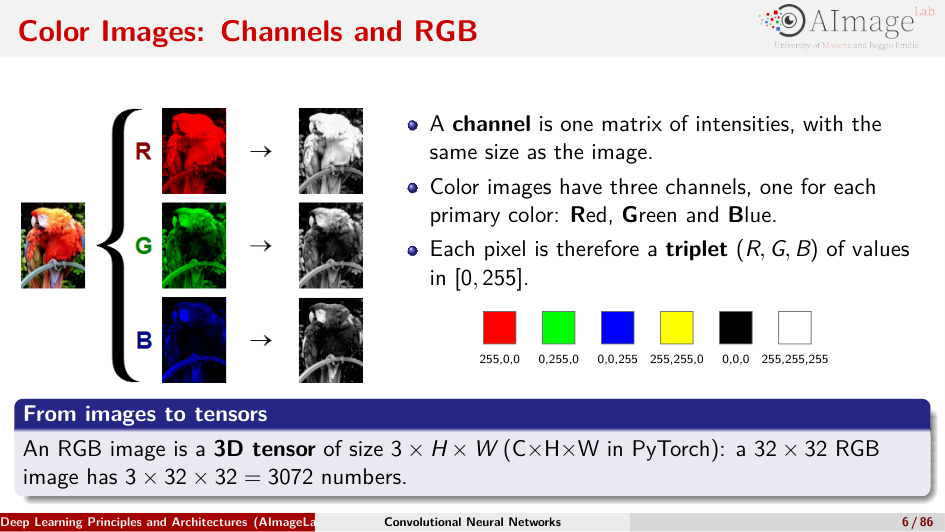
\includegraphics[keepaspectratio]{figure/fig_1e8ae7db40c977b5.png}}
\caption{Slide 6 -- Color Images: Channels and RGB}
\end{figure}
% END F02-B0023

% BEGIN F02-B0024
Un\textquotesingle immagine a colori non può essere descritta da una singola matrice bidimensionale: essa si articola in \textbf{tre matrici spaziali parallele sovrapposte}, denominate \textbf{canali} (\emph{channels}), ciascuna di dimensioni \(H \times W\), che registrano individualmente il contributo di intensità del rispettivo spettro cromatico nell\textquotesingle intervallo \([0, 255]\). Ciascun pixel è identificato da una terna ordinata \((R, G, B)\).
% END F02-B0024

% BEGIN F02-B0025
Nel framework formale del Deep Learning e in librerie come PyTorch, un\textquotesingle immagine RGB viene rappresentata mediante un \textbf{tensore tridimensionale} di dimensioni:
% END F02-B0025

% BEGIN F02-B0026
\begin{center}
\begin{adjustbox}{max width=\linewidth}
$\displaystyle 
\boxed{X \in \mathbb{R}^{C \times H \times W}}
$
\end{adjustbox}
\end{center}
% END F02-B0026

% BEGIN F02-B0027
dove \(C = 3\) indica il numero di canali, \(H\) l\textquotesingle altezza e \(W\) la larghezza (notazione \emph{channels-first}, standard per PyTorch, a differenza della convenzione \emph{channels-last} \(H \times W \times C\) utilizzata storicamente da altre librerie). Ad esempio, una minuscola immagine RGB di dimensioni \(32 \times 32\) (come quelle del benchmark CIFAR-10) è formata da:
% END F02-B0027

% BEGIN F02-B0028
\begin{center}
\begin{adjustbox}{max width=\linewidth}
$\displaystyle 
3 \times 32 \times 32 = 3072 \text{ valori scalari}
$
\end{adjustbox}
\end{center}
% END F02-B0028

% BEGIN F02-B0029
\begin{center}\rule{0.5\linewidth}{0.5pt}\end{center}
% END F02-B0029

% BEGIN F02-B0030
\section{Paradigmi di Computer Vision ed Evoluzione Storica (slide 7--11)}\label{f02-r110}
% END F02-B0030

% BEGIN F02-B0031
La disciplina della \textbf{Computer Vision (CV)} si colloca all\textquotesingle intersezione tra l\textquotesingle analisi del segnale e l\textquotesingle intelligenza artificiale, ponendosi l\textquotesingle obiettivo formale di estrarre conoscenza e descrizioni semantiche esplicite a partire da flussi visivi ("elaborare immagini per ottenere dati comprensibili e decisioni operative").
% END F02-B0031

% BEGIN F02-B0032
\begin{figure}[H]
\centering
\pandocbounded{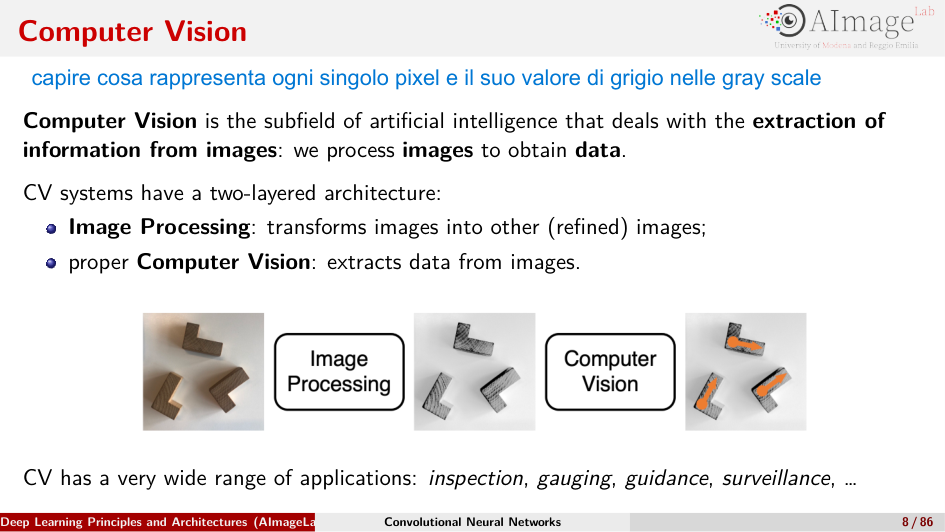
\includegraphics[keepaspectratio]{figure/fig_652c53cda8fe133d.png}}
\caption{Slide 8 -- Computer Vision}
\end{figure}
% END F02-B0032

% BEGIN F02-B0033
Nella tassonomia accademica dei sistemi visivi si distingue rigorosamente tra due livelli gerarchici di elaborazione:
% END F02-B0033

% BEGIN F02-B0034
\begin{itemize}
\tightlist
\item
  \textbf{Image Processing (Elaborazione delle immagini)}: trasforma immagini di ingresso in altre immagini modificate o raffinate (ad esempio aumentando il contrasto, sopprimendo il rumore di acquisizione o correggendo aberrazioni cromatiche). Opera sui pixel trattandoli come entità numeriche astratte, senza comprendere in alcun modo il significato semantico degli oggetti rappresentati o la geometria tridimensionale della scena.
\item
  \textbf{Computer Vision propriamente detta}: opera a un livello di astrazione semantica superiore. Il suo fine non è alterare i pixel, bensì interpretare cosa quei valori numerici rappresentino nel mondo reale (compiti di riconoscimento, misurazione volumetrica, guida di veicoli autonomi, videosorveglianza e controllo qualità industriale).
\end{itemize}
% END F02-B0034

% BEGIN F02-B0035
\subsection{La Scomposizione Classica in Due Stadi (slide 9)}\label{f02-r121}
% END F02-B0035

% BEGIN F02-B0036
Poiché lo spazio delle configurazioni di pixel grezzi presenta una dimensionalità astronomica, la visione artificiale classica ha storicamente frammentato il problema in due stadi sequenziali disaccoppiati:
% END F02-B0036

% BEGIN F02-B0037
\pandocbounded{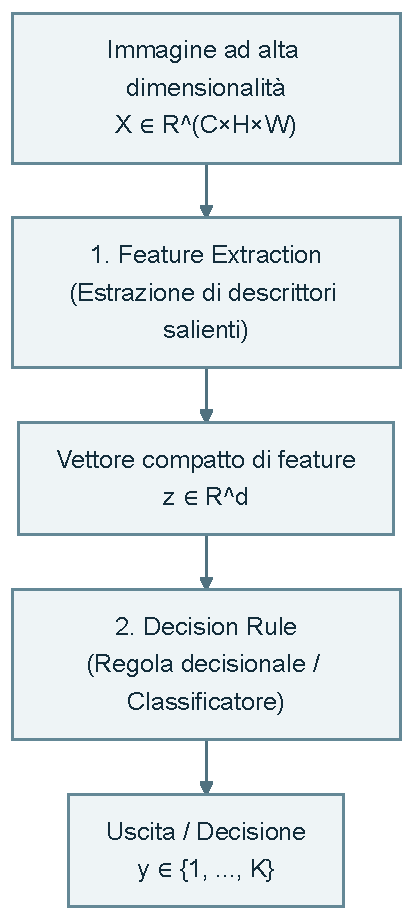
\includegraphics[keepaspectratio]{figure/diagramma_f02_02.pdf}}
% END F02-B0037

% BEGIN F02-B0038
\begin{enumerate}
\def\labelenumi{\arabic{enumi}.}
\tightlist
\item
  \textbf{Feature Extraction (Estrazione delle caratteristiche)}: riduce la dimensionalità grezza dell\textquotesingle immagine calcolando una rappresentazione compatta ed espressiva (il vettore di \emph{feature}), progettata per trattenere le informazioni salienti per lo specifico compito (es. profili dei contorni, orientamento dei gradienti, consistenza della trama) scartando le variazioni irrilevanti (come cambi di luminosità globale).
\item
  \textbf{Decision Rule (Regola decisionale)}: prende in ingresso il vettore di feature compatto e formula il verdetto finale (assegnazione della classe, regressione delle coordinate o stima di parametri).
\end{enumerate}
% END F02-B0038

% BEGIN F02-B0039
\subsection{Le Tre Ere Paradigmatiche della Visione Artificiale (slide 10--11)}\label{f02-r136}
% END F02-B0039

% BEGIN F02-B0040
L\textquotesingle evoluzione della Computer Vision dagli anni \textquotesingle70 a oggi è scandita da tre paradigmi metodologici:
% END F02-B0040

% BEGIN F02-B0041
\begin{figure}[H]
\centering
\pandocbounded{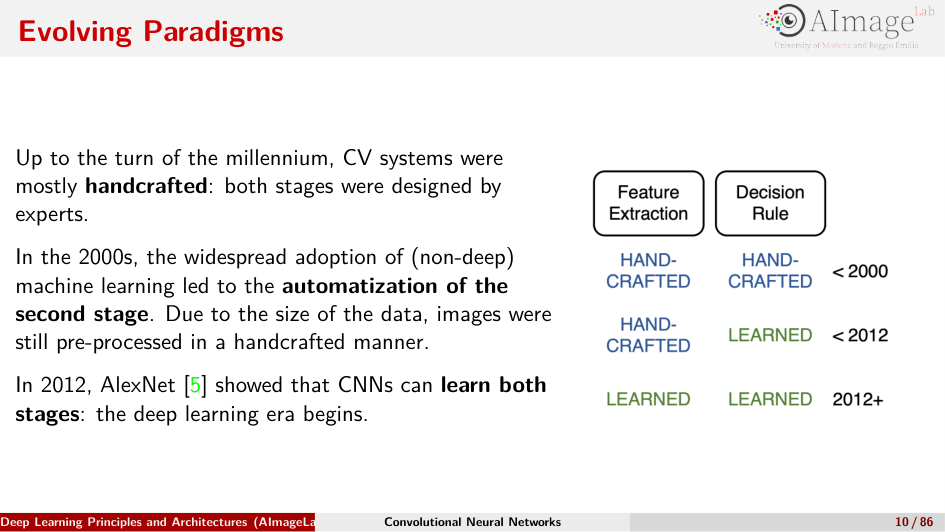
\includegraphics[keepaspectratio]{figure/fig_28b47cf024ee150a.png}}
\caption{Slide 10 -- Evolving Paradigms}
\end{figure}
% END F02-B0041

% BEGIN F02-B0042
\begin{longtable}[]{@{}
  >{\raggedright\arraybackslash}p{(\linewidth - 6\tabcolsep) * \real{0.2500}}
  >{\raggedright\arraybackslash}p{(\linewidth - 6\tabcolsep) * \real{0.2500}}
  >{\raggedright\arraybackslash}p{(\linewidth - 6\tabcolsep) * \real{0.2500}}
  >{\raggedright\arraybackslash}p{(\linewidth - 6\tabcolsep) * \real{0.2500}}@{}}
\toprule\noalign{}
\begin{minipage}[b]{\linewidth}\raggedright
Periodo Storico
\end{minipage} & \begin{minipage}[b]{\linewidth}\raggedright
Feature Extraction
\end{minipage} & \begin{minipage}[b]{\linewidth}\raggedright
Decision Rule
\end{minipage} & \begin{minipage}[b]{\linewidth}\raggedright
Caratteristiche del Modello
\end{minipage} \\
\midrule\noalign{}
\endhead
\bottomrule\noalign{}
\endlastfoot
\textbf{Fino al 2000} & Progettata a mano (\emph{Handcrafted}) & Progettata a mano (\emph{Handcrafted}) & Regole euristiche basate su soglie fisse, allineamento di maschere rigide e modelli geometrici analitici formulati dall\textquotesingle esperto umano. \\
\textbf{Anni 2000 -- 2012} & Progettata a mano (\emph{Handcrafted}) & Appresa statisticamente (\emph{Learned}) & Descrittori ingegnerizzati complessi (es. SIFT, HOG, SURF) combinati con classificatori statistici di Machine Learning (SVM, Random Forest, AdaBoost). \\
\textbf{2012 -- Oggi} & \textbf{Appresa congiuntamente dai dati} & \textbf{Appresa congiuntamente dai dati} & \textbf{Deep Learning End-to-End}: reti neurali convoluzionali profonde (spartiacque storico: \textbf{AlexNet}, 2012). Estrazione delle feature e classificazione sono unificate e ottimizzate simultaneamente mediante differenziazione automatica. \\
\end{longtable}
% END F02-B0042

% BEGIN F02-B0043
\begin{figure}[H]
\centering
\pandocbounded{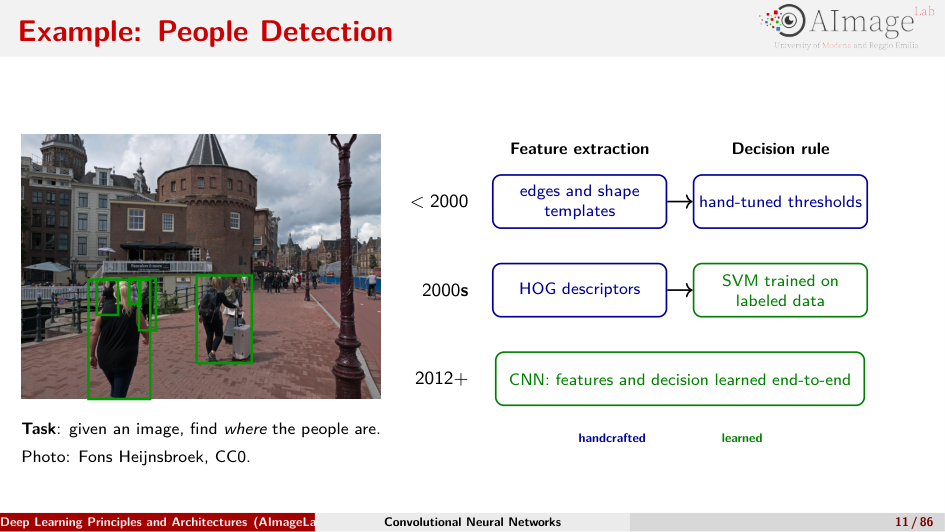
\includegraphics[keepaspectratio]{figure/fig_e8accdee14bba428.png}}
\caption{Slide 11 -- Example: People Detection}
\end{figure}
% END F02-B0043

% BEGIN F02-B0044
L\textquotesingle esempio emblematico mostrato nella Slide 11 riguarda il compito di \textbf{rilevamento di pedoni (People Detection)}: * \textbf{Prima del 2000}: si disegnavano a mano delle sagome geometriche standard (\emph{template} stilizzati del corpo umano) e le si faceva scorrere sull\textquotesingle immagine, verificando mediante correlazione visiva se la sovrapposizione superava una certa soglia arbitraria. * \textbf{Negli anni 2000}: si calcolavano i descrittori \textbf{HOG (Histogram of Oriented Gradients)} per catturare le direzioni dominanti dei gradienti lungo la silhouette della persona, e si addestrava un classificatore Support Vector Machine (SVM) per discriminare tra la classe pedone e lo sfondo. * \textbf{Con l\textquotesingle avvento di AlexNet nel 2012}: si alimenta l\textquotesingle immagine direttamente a una rete convoluzionale profonda; il modello apprende dai dati grezzi sia i filtri per riconoscere la sagoma sia i pesi per la classificazione finale, superando nettamente ogni prestazione manuale precedente.
% END F02-B0044

% BEGIN F02-B0045
\begin{center}\rule{0.5\linewidth}{0.5pt}\end{center}
% END F02-B0045

% BEGIN F02-B0046
\section{Limiti del Multilayer Perceptron per Dati Visivi (slide 12--18)}\label{f02-r157}
% END F02-B0046

% BEGIN F02-B0047
Le reti neurali convoluzionali non ripudiano la matematica del Multilayer Perceptron (\hyperref[fonte01]{Multilayer Perceptron}), bensì ne condividono l\textquotesingle impalcatura teorica fondamentale (Slide 13):
% END F02-B0047

% BEGIN F02-B0048
\begin{itemize}
\tightlist
\item
  Sono costituite da strati di neuroni artificiali dotati di pesi e bias apprendibili.
\item
  Ciascun neurone calcola una trasformazione lineare (prodotto scalare tra pesi e input) seguita da una funzione di attivazione non lineare.
\item
  L\textquotesingle intera architettura definisce una \textbf{funzione continua e differenziabile a tratti}, addestrabile end-to-end tramite l\textquotesingle algoritmo di retropropagazione del gradiente (\textbf{Backpropagation}).
\end{itemize}
% END F02-B0048

% BEGIN F02-B0049
Tuttavia, l\textquotesingle applicazione diretta di un MLP alle immagini svela immediatamente limiti rilevanti, sia di natura computazionale sia di compatibilità geometrica.
% END F02-B0049

% BEGIN F02-B0050
\pandocbounded{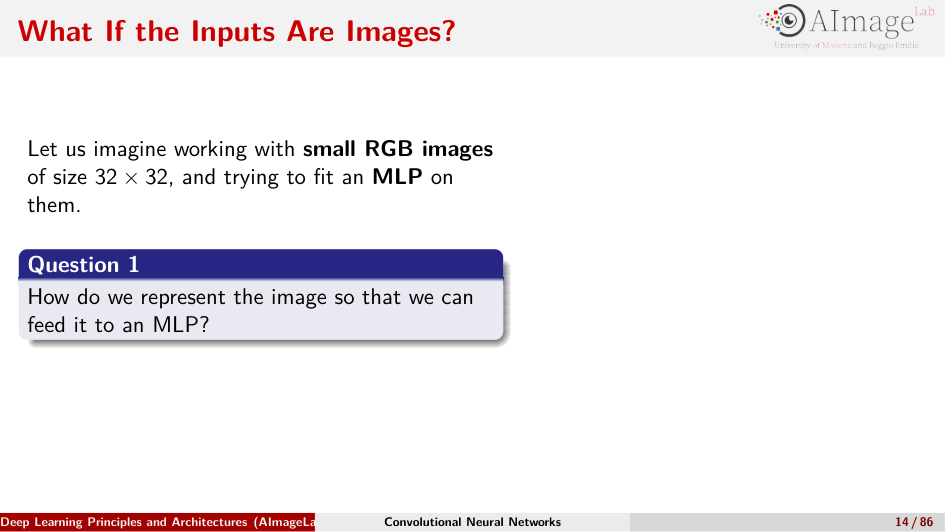
\includegraphics[keepaspectratio]{figure/fig_8e5f42de7af09f0f.png}} \pandocbounded{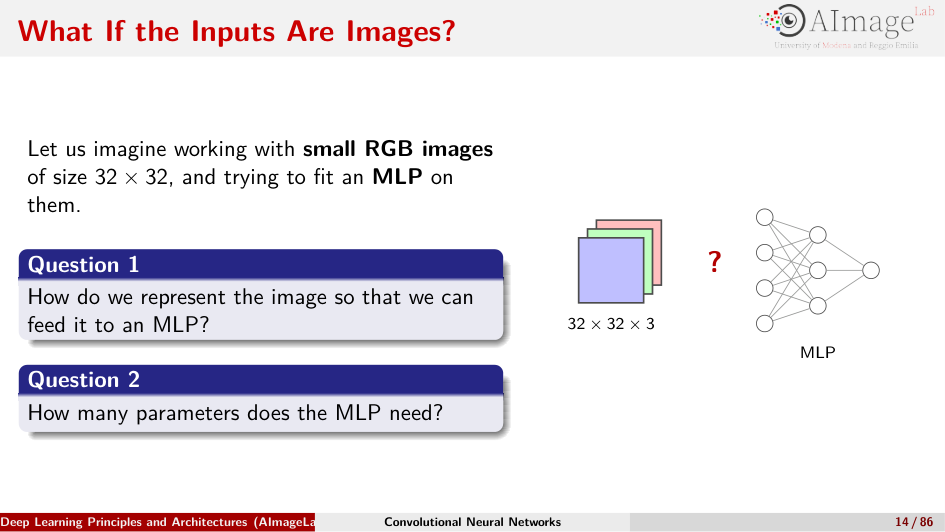
\includegraphics[keepaspectratio]{figure/fig_a00db1b9d9871c04.png}}
% END F02-B0050

% BEGIN F02-B0051
\subsection{Esplosione Parametrica e Inefficienza Computazionale (slide 14--16)}\label{f02-r170}
% END F02-B0051

% BEGIN F02-B0052
Nelle slide 14 e 15 vengono poste due domande fondamentali:
% END F02-B0052

% BEGIN F02-B0053
\begin{quote}
\textbf{Domanda 1:} Come rappresentiamo un\textquotesingle immagine in modo da poterla fornire in ingresso a un MLP?\\
\textbf{Domanda 2:} Di quanti parametri ha bisogno l\textquotesingle MLP per elaborarla?
\end{quote}
% END F02-B0053

% BEGIN F02-B0054
La risposta alla Domanda 1 impone l\textquotesingle operazione di \textbf{appiattimento (Flattening)}: poiché i neuroni di uno strato denso (Fully Connected) accettano unicamente ingressi monodimensionali, la matrice o il tensore dell\textquotesingle immagine deve essere "srotolato" in un unico vettore colonna \(x \in \mathbb{R}^D\). Per una matrice RGB \(32 \times 32\):
% END F02-B0054

% BEGIN F02-B0055
\begin{center}
\begin{adjustbox}{max width=\linewidth}
$\displaystyle 
x \in \mathbb{R}^{3 \cdot 32 \cdot 32} = \mathbb{R}^{3072}
$
\end{adjustbox}
\end{center}
% END F02-B0055

% BEGIN F02-B0056
La risposta alla Domanda 2 svela la drammatica esplosione del numero di parametri. Consideriamo un MLP dotato di un singolo strato nascosto estremamente modesto, composto da soli \(M = 512\) neuroni:
% END F02-B0056

% BEGIN F02-B0057
\begin{figure}[H]
\centering
\pandocbounded{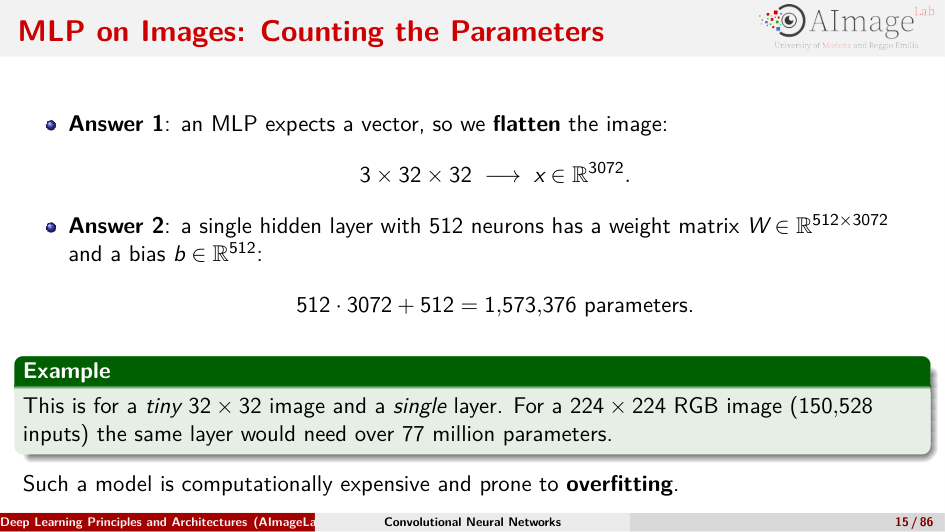
\includegraphics[keepaspectratio]{figure/fig_80cfb03b700de293.png}}
\caption{Slide 16 -- MLP on Images: Counting the Parameters}
\end{figure}
% END F02-B0057

% BEGIN F02-B0058
La matrice dei pesi dello strato è \(W \in \mathbb{R}^{512 \times 3072}\) e il vettore dei bias è \(b \in \mathbb{R}^{512}\). Il conteggio esatto dei parametri liberi risulta:
% END F02-B0058

% BEGIN F02-B0059
\begin{center}
\begin{adjustbox}{max width=\linewidth}
$\displaystyle 
\text{Parametri} = (512 \times 3072) + 512 = 1.572.864 + 512 = \mathbf{1.573.376}
$
\end{adjustbox}
\end{center}
% END F02-B0059

% BEGIN F02-B0060
Oltre un milione e mezzo di parametri per un\textquotesingle immagine giocattolo di appena \(32 \times 32\) pixel! Se consideriamo una risoluzione comune per la visione artificiale moderna (come lo standard ImageNet da \(224 \times 224\) pixel RGB), il vettore di ingresso contiene:
% END F02-B0060

% BEGIN F02-B0061
\begin{center}
\begin{adjustbox}{max width=\linewidth}
$\displaystyle 
D = 3 \times 224 \times 224 = 150.528 \text{ componenti}
$
\end{adjustbox}
\end{center}
% END F02-B0061

% BEGIN F02-B0062
Collegando questo ingresso agli stessi 512 neuroni nascosti, il numero di parametri lievita a:
% END F02-B0062

% BEGIN F02-B0063
\begin{center}
\begin{adjustbox}{max width=\linewidth}
$\displaystyle 
\text{Parametri} = (512 \times 150.528) + 512 = 77.070.336 + 512 = \mathbf{77.070.848}
$
\end{adjustbox}
\end{center}
% END F02-B0063

% BEGIN F02-B0064
Uno strato singolo richiede oltre \textbf{77 milioni di pesi}. Per un\textquotesingle immagine ad alta definizione (\(1000 \times 1000\) pixel) e uno strato nascosto proporzionato, si supererebbe ampiamente il miliardo di parametri per un solo livello. Questa mole di pesi ha un costo elevato di calcolo e memoria e può rendere più difficile generalizzare con pochi dati; il numero dei pesi da solo non dimostra overfitting.
% END F02-B0064

% BEGIN F02-B0065
\subsection{Criticità Strutturali dell\textquotesingle MLP sulle Immagini (slide 17)}\label{f02-r207}
% END F02-B0065

% BEGIN F02-B0066
Al di là del costo computazionale, l\textquotesingle MLP denso non incorpora esplicitamente la struttura geometrica intrinseca dei dati visivi:
% END F02-B0066

% BEGIN F02-B0067
\begin{figure}[H]
\centering
\pandocbounded{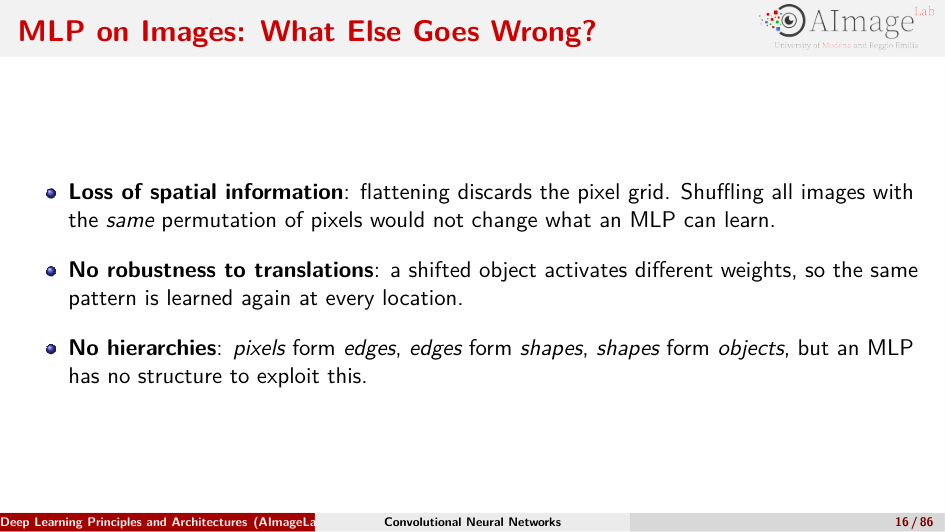
\includegraphics[keepaspectratio]{figure/fig_f907e401d7aababd.png}}
\caption{Slide 17 -- MLP on Images: What Else Goes Wrong?}
\end{figure}
% END F02-B0067

% BEGIN F02-B0068
\begin{enumerate}
\def\labelenumi{\arabic{enumi}.}
\tightlist
\item
  \textbf{Perdita della struttura topologica spaziale (\emph{Loss of spatial information})}: Lo srotolamento è invertibile e non elimina i valori dei pixel; è il livello denso a non imporre esplicitamente la geometria della griglia. In un vettore piatto, la distanza tra il pixel \((0, 0)\) e il suo vicino adiacente \((0, 1)\) è trattata con la medesima neutralità della distanza tra il pixel \((0, 0)\) e l\textquotesingle angolo opposto \((31, 31)\). Se applicassimo a tutte le immagini di addestramento una permutazione casuale fissa di pixel, l\textquotesingle immagine risulterebbe incomprensibile per un essere umano, ma la capacità di apprendimento di un MLP rimarrebbe esattamente invariata.
\item
  \textbf{Mancanza di invarianza/equivarianza alla traslazione (\emph{No translation robustness})}: in un MLP, a ogni indice del vettore di ingresso corrisponde un peso distinto. Se un pattern visivo (ad esempio il volto di un gatto) si sposta dall\textquotesingle angolo superiore sinistro a quello inferiore destro dell\textquotesingle immagine, esso attiverà componenti del vettore e pesi completamente diversi. L\textquotesingle MLP non impone la condivisione spaziale dei pesi: apprendere lo stesso pattern in posizioni diverse può richiedere più esempi.
\item
  \textbf{Assenza di una gerarchia locale imposta dall'architettura}: il mondo visivo naturale è strutturato secondo una gerarchia compositiva (i pixel formano contorni, i contorni si combinano in forme geometriche, le forme compongono parti di oggetti e le parti formano l\textquotesingle oggetto intero). La connettività densa e uniforme di un MLP non fornisce alcun vincolo architetturale che guidi la rete verso questa progressiva astrazione.
\end{enumerate}
% END F02-B0068

% BEGIN F02-B0069
\subsection{Le Proprietà Fisiche delle Immagini e l\textquotesingle Inductive Bias (slide 18)}\label{f02-r217}
% END F02-B0069

% BEGIN F02-B0070
I dati visivi naturali possiedono due regolarità utili in molti compiti:
% END F02-B0070

% BEGIN F02-B0071
\begin{enumerate}
\def\labelenumi{\arabic{enumi}.}
\tightlist
\item
  \textbf{Proprietà del segnale: Località e Continuità Spaziale (\emph{Spatial Locality})}: la luce riflessa dagli oggetti del mondo fisico varia nello spazio in modo continuo. Di conseguenza, i pixel spazialmente vicini presentano una \textbf{fortissima correlazione statistica}: il valore di intensità di un pixel \(I(x, y)\) fornisce un\textquotesingle enorme quantità di informazione sul valore del pixel contiguo \(I(x+1, y)\), mentre pixel a grande distanza hanno correlazione via via decrescente.
\item
  \textbf{Proprietà semantica: Indipendenza del contenuto dalla posizione (\emph{Translation Invariance})}: l\textquotesingle identità semantica di un oggetto è invariante rispetto alla sua collocazione nel fotogramma. Un\textquotesingle automobile rimane un\textquotesingle automobile sia che si trovi al centro, a destra o a sinistra dell\textquotesingle inquadratura.
\end{enumerate}
% END F02-B0071

% BEGIN F02-B0072
\begin{figure}[H]
\centering
\pandocbounded{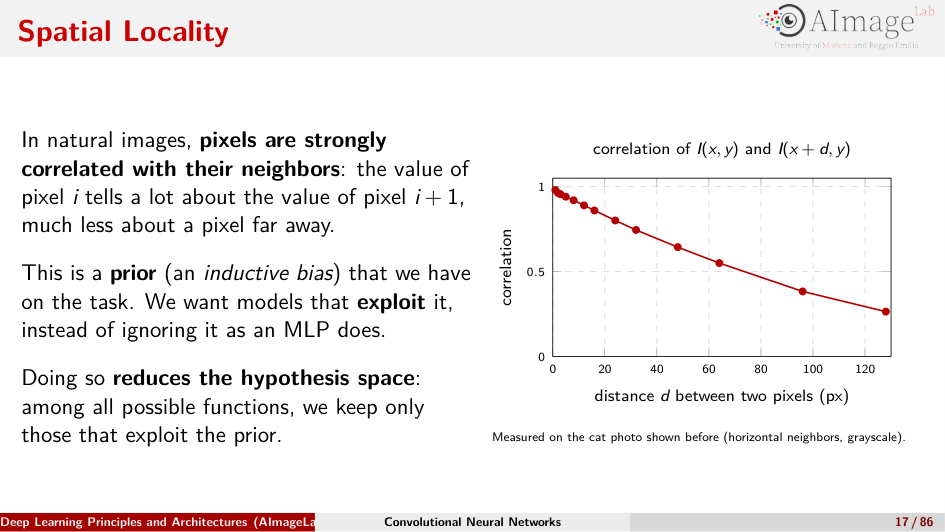
\includegraphics[keepaspectratio]{figure/fig_3f2731566306d237.png}}
\caption{Slide 18 -- Spatial Locality}
\end{figure}
% END F02-B0072

% BEGIN F02-B0073
Il grafico mostrato nella Slide 18 traccia la correlazione empirica tra \(I(x, y)\) e \(I(x+d, y)\) in funzione della distanza euclidea \(d\) in pixel: per distanze minime (\(d \to 0\)) la correlazione è quasi unitaria, per poi decadere rapidamente al crescere di \(d\).
% END F02-B0073

% BEGIN F02-B0074
L\textquotesingle integrazione di queste due evidenze nella struttura di una rete neurale costituisce un potente \textbf{Inductive Bias} (bias induttivo): anziché costringere l\textquotesingle algoritmo a cercare una funzione predittiva nell\textquotesingle intero e sterminato spazio di tutte le funzioni astratte possibili (spazio delle ipotesi dell\textquotesingle MLP), restringiamo a priori l\textquotesingle architettura alle sole funzioni che rispettano la località spaziale e l\textquotesingle invarianza traslazionale. Ciò abbatte la complessità di calcolo e può favorire la generalizzazione quando queste ipotesi sono appropriate.
% END F02-B0074

% BEGIN F02-B0075
\begin{center}\rule{0.5\linewidth}{0.5pt}\end{center}
% END F02-B0075

% BEGIN F02-B0076
\section{Principi Architetturali e Ispirazione Biologica (slide 19--23)}\label{f02-r232}
% END F02-B0076

% BEGIN F02-B0077
Le CNN riprendono un\textquotesingle intuizione della visione biologica: combinare risposte locali in rappresentazioni via via più complesse. Il campo recettivo descrive la porzione di ingresso che può influenzare un\textquotesingle unità. L\textquotesingle analogia fra elaborazione locale e riconoscimento globale motiva l\textquotesingle architettura, ma non significa che la rete riproduca esattamente il sistema visivo.
% END F02-B0077

% BEGIN F02-B0078
\begin{figure}[H]
\centering
\pandocbounded{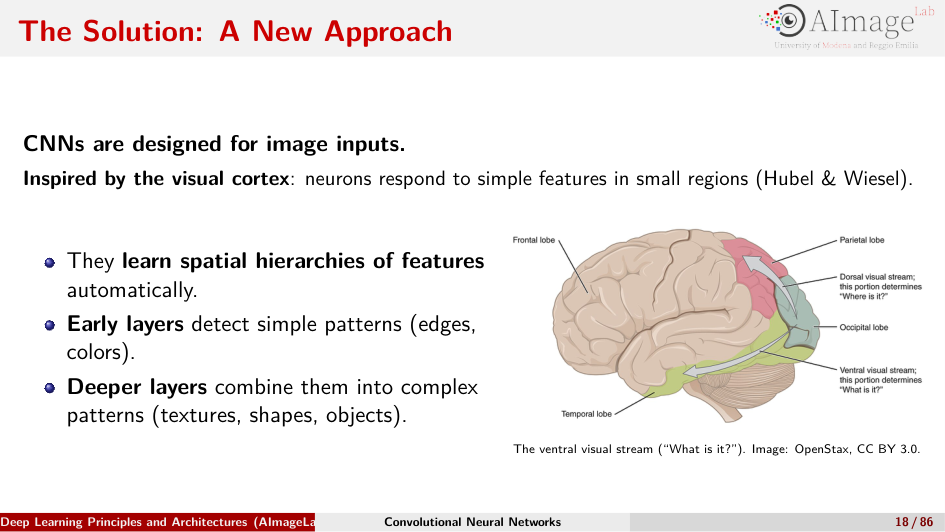
\includegraphics[keepaspectratio]{figure/fig_1a4c9fb2bbf3f2dc.png}}
\caption{Slide 19 -- Un approccio locale e gerarchico}
\end{figure}
% END F02-B0078

% BEGIN F02-B0079
\subsection{I Tre Blocchi Costruttivi della CNN (slide 20--22)}\label{f02-r238}
% END F02-B0079

% BEGIN F02-B0080
Per emulare artificialmente questo principio di calcolo, una rete convoluzionale standard combina tre blocchi architetturali (Slide 21):
% END F02-B0080

% BEGIN F02-B0081
\begin{enumerate}
\def\labelenumi{\arabic{enumi}.}
\tightlist
\item
  \textbf{Livelli Convoluzionali (Convolutional Layers)}: applicano banchi di filtri locali lineari che scorrono sull\textquotesingle immagine per estrarre mappe di feature, sfruttando la connettività sparsa e la condivisione dei parametri.
\item
  \textbf{Funzioni di Attivazione (Activation Functions)}: introducono non linearità puntuali indispensabili per impedire il collasso algebrico degli strati e consentire l\textquotesingle apprendimento di funzioni complesse.
\item
  \textbf{Livelli di Pooling (Pooling Layers)}: operano un sottocampionamento spaziale progressivo, riducendo la risoluzione geometrica delle mappe e allargando il campo recettivo per gli strati successivi.
\end{enumerate}
% END F02-B0081

% BEGIN F02-B0082
\begin{figure}[H]
\centering
\pandocbounded{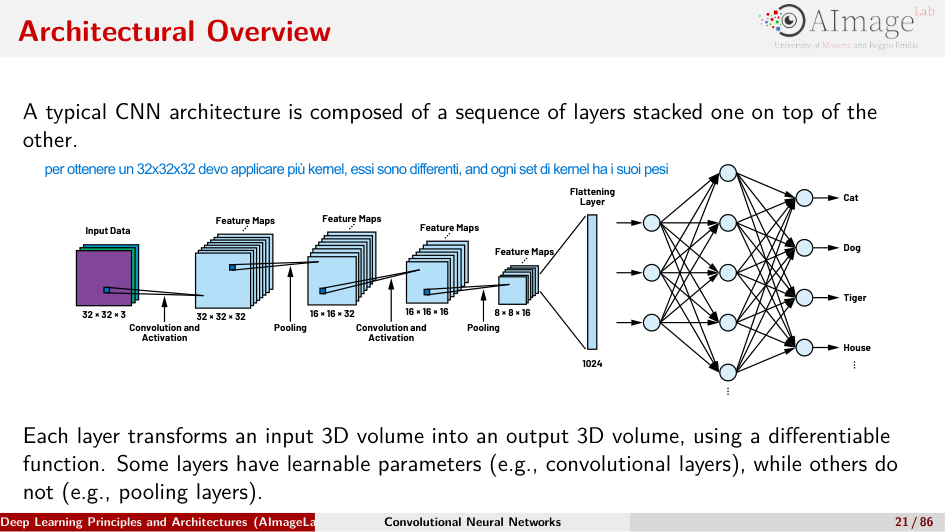
\includegraphics[keepaspectratio]{figure/fig_085569bebb2d4f0a.png}}
\caption{Slide 22 -- Architectural Overview}
\end{figure}
% END F02-B0082

% BEGIN F02-B0083
Lo schema complessivo di una classica architettura convoluzionale (Slide 22) si struttura secondo la seguente sequenza:
% END F02-B0083

% BEGIN F02-B0084
\pandocbounded{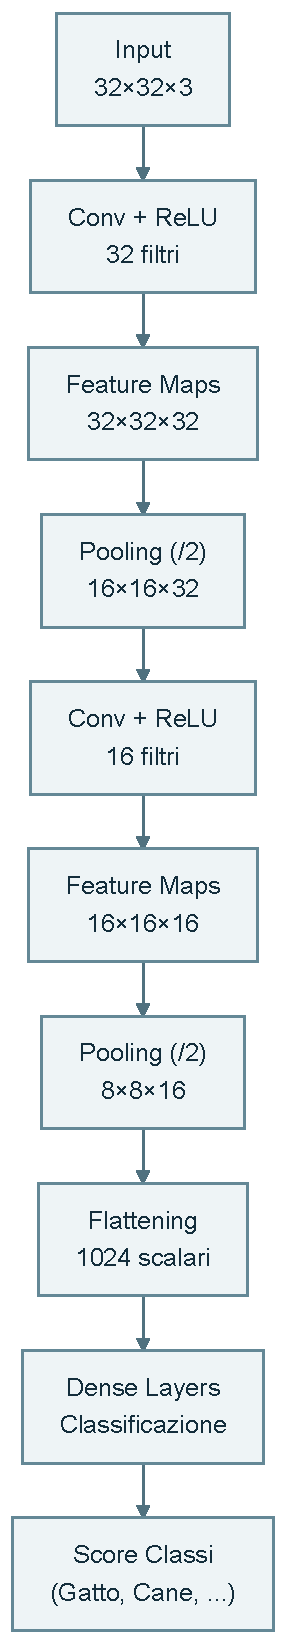
\includegraphics[keepaspectratio]{figure/diagramma_f02_03.pdf}}
% END F02-B0084

% BEGIN F02-B0085
Un tensore di ingresso (es. \(32 \times 32 \times 3\)) viene elaborato dal primo strato convoluzionale: le dimensioni spaziali rimangono controllate mentre il numero di canali viene espanso (es. a 32 canali). Il livello di pooling dimezza la risoluzione spaziale (portandola a \(16 \times 16\)), mantenendo inalterata la profondità dei canali. Una seconda convoluzione rielabora i canali (portandoli a 16), e un successivo pooling riduce la griglia a \(8 \times 8 \times 16\).
% END F02-B0085

% BEGIN F02-B0086
Al termine dello stadio estrattivo, il volume compatto risultante viene appiattito in un vettore monodimensionale di feature ad alto livello (\(8 \times 8 \times 16 = 1024\) elementi), che viene infine classificato da uno strato denso standard (MLP). \textbf{Il sistema è continuo e differenziabile a tratti}: il gradiente della funzione di perdita fluisce a ritroso lungo tutti i livelli, aggiornando simultaneamente sia i pesi del classificatore sia i parametri di ciascun filtro convoluzionale.
% END F02-B0086

% BEGIN F02-B0087
\begin{center}\rule{0.5\linewidth}{0.5pt}\end{center}
% END F02-B0087

% BEGIN F02-B0088
\section{Operatori su Immagini e Sistemi Lineari Traslazione-Invarianti (LSI) (slide 24--34)}\label{f02-r269}
% END F02-B0088

% BEGIN F02-B0089
Per formalizzare matematicamente il funzionamento del livello convoluzionale occorre comprendere la natura degli operatori bidimensionali del processamento numerico dei segnali visivi (Slide 24):
% END F02-B0089

% BEGIN F02-B0090
\begin{itemize}
\tightlist
\item
  \textbf{Operatori puntuali (Point operators)}: il valore del pixel di uscita \(o(x, y)\) dipende esclusivamente dal valore assunto dal pixel di ingresso nella medesima coordinata \(i(x, y)\). Esempi tipici sono la correzione di contrasto/luminosità e la correzione gamma con parametri fissati.
\item
  \textbf{Operatori locali o filtri spaziali (Local operators)}: il valore del pixel di uscita \(o(x, y)\) viene determinato elaborando congiuntamente un insieme compatto di pixel appartenenti a un intorno geometrico (un vicinato locale) circostante la coordinata \((x, y)\).
\end{itemize}
% END F02-B0090

% BEGIN F02-B0091
\begin{figure}[H]
\centering
\pandocbounded{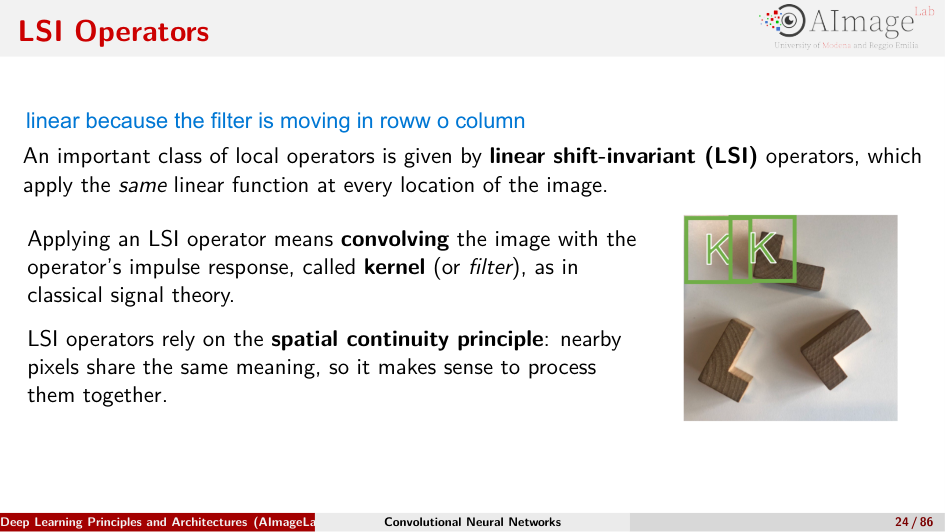
\includegraphics[keepaspectratio]{figure/fig_cf3c8b044f550533.png}}
\caption{Slide 25 -- LSI Operators}
\end{figure}
% END F02-B0091

% BEGIN F02-B0092
Una classe fondamentale di operatori locali è costituita dagli \textbf{operatori lineari e invarianti alla traslazione} (\textbf{LSI - Linear Shift-Invariant operators}, Slide 25). Un operatore locale \(\mathcal{T}\) si dice LSI se soddisfa due condizioni: 1. \textbf{Linearità}: \(\mathcal T(aX+bY)=a\mathcal T(X)+b\mathcal T(Y)\). L\textquotesingle annotazione della slide 25 che collega «linear» al movimento lungo righe e colonne non è corretta: la linearità riguarda la sovrapposizione dei segnali. Un filtro massimo scorre allo stesso modo ma non è lineare. Un bias non nullo rende la trasformazione affine. 2. \textbf{Invarianza alla traslazione (Shift-Invariance)}: applica \textbf{la medesima identica funzione} a ogni posizione spaziale dell\textquotesingle immagine, indipendentemente dalla posizione della finestra.
% END F02-B0092

% BEGIN F02-B0093
Applicare un operatore LSI a un\textquotesingle immagine equivale algebricamente a eseguire la \textbf{convoluzione} tra l\textquotesingle immagine e la risposta impulsiva dell\textquotesingle operatore, denominata \textbf{kernel} (o filtro).
% END F02-B0093

% BEGIN F02-B0094
\begin{figure}[H]
\centering
\pandocbounded{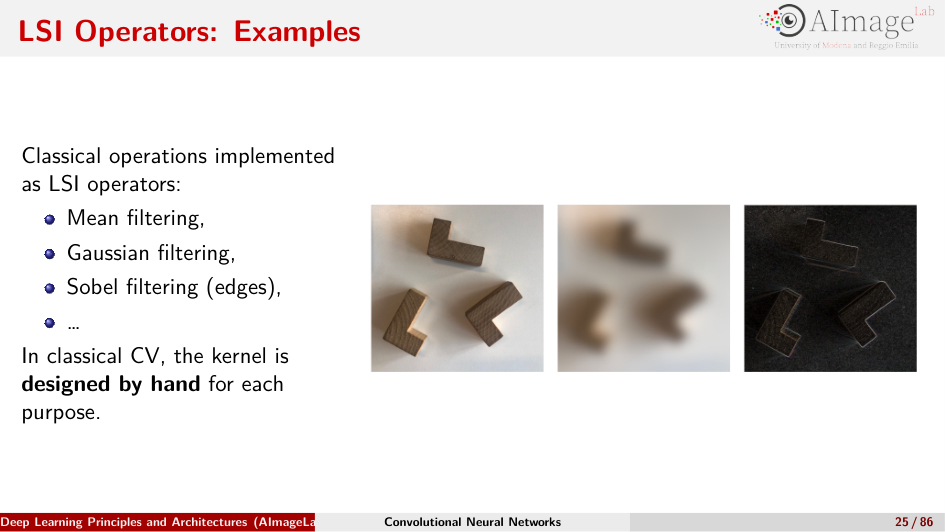
\includegraphics[keepaspectratio]{figure/fig_32595760ed9de60f.png}}
\caption{Slide 26 -- LSI Operators: Examples}
\end{figure}
% END F02-B0094

% BEGIN F02-B0095
Tra gli operatori LSI classici ampiamente impiegati nella Computer Vision pre-deep learning figurano (Slide 26): * \textbf{Filtro di media (Mean filtering)}: calcola la media aritmetica non pesata dei pixel nel vicinato, producendo un effetto di sfocatura (\emph{smoothing}). * \textbf{Filtro gaussiano (Gaussian filtering)}: assegna pesi decrescenti a campana gaussiana in base alla distanza dal centro, riducendo il rumore ad alta frequenza preservando meglio i contorni. * \textbf{Filtri derivativi (es. Sobel, Prewitt)}: calcolano le differenze discrete di intensità tra pixel adiacenti. Poiché la derivata prima spaziale evidenzia le discontinuità repentine di intensità, questi filtri estraggono i contorni (\emph{edges}) degli oggetti.
% END F02-B0095

% BEGIN F02-B0096
\subsection{\texorpdfstring{Esempio Calcolato a Mano: Filtro di Media \(3 \times 3\) (slide 27--31)}{Esempio Calcolato a Mano: Filtro di Media 3 \textbackslash times 3 (slide 27--31)}}\label{f02-r291}
% END F02-B0096

% BEGIN F02-B0097
Nelle slide 27--31 viene illustrata l\textquotesingle applicazione di un filtro di media con kernel \(3 \times 3\) su una porzione di immagine reale in scala di grigi.
% END F02-B0097

% BEGIN F02-B0098
\begin{figure}[H]
\centering
\pandocbounded{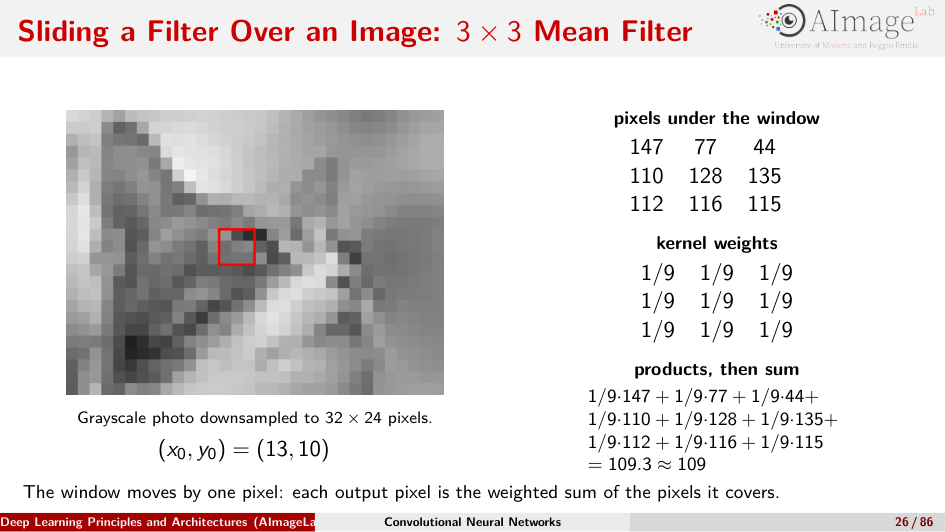
\includegraphics[keepaspectratio]{figure/fig_f50ee7901473242e.png}}
\caption{Slide 27 -- Sliding a Filter Over an Image: 3 × 3 Mean Filter}
\end{figure}
% END F02-B0098

% BEGIN F02-B0099
Il kernel del filtro di media è una matrice quadrata \(3 \times 3\) i cui coefficienti sommano a 1:
% END F02-B0099

% BEGIN F02-B0100
\begin{center}
\begin{adjustbox}{max width=\linewidth}
$\displaystyle 
K = \begin{bmatrix}
1/9 & 1/9 & 1/9 \\
1/9 & 1/9 & 1/9 \\
1/9 & 1/9 & 1/9
\end{bmatrix}
$
\end{adjustbox}
\end{center}
% END F02-B0100

% BEGIN F02-B0101
Alla coordinata spaziale iniziale \((x_0, y_0) = (13, 10)\), i pixel dell\textquotesingle immagine coperti dalla finestra del filtro sono:
% END F02-B0101

% BEGIN F02-B0102
\begin{center}
\begin{adjustbox}{max width=\linewidth}
$\displaystyle 
P_{(13, 10)} = \begin{bmatrix}
147 & 77 & 44 \\
110 & 128 & 135 \\
112 & 116 & 115
\end{bmatrix}
$
\end{adjustbox}
\end{center}
% END F02-B0102

% BEGIN F02-B0103
L\textquotesingle operazione locale consiste nel moltiplicare elemento per elemento ciascun pixel per il corrispondente coefficiente del kernel e sommare i 9 prodotti risultanti:
% END F02-B0103

% BEGIN F02-B0104
\begin{center}
\begin{adjustbox}{max width=\linewidth}
$\displaystyle 
\begin{aligned}
\text{Output} &= \frac{1}{9}(147) + \frac{1}{9}(77) + \frac{1}{9}(44) + \frac{1}{9}(110) + \frac{1}{9}(128) + \frac{1}{9}(135) + \frac{1}{9}(112) + \frac{1}{9}(116) + \frac{1}{9}(115) \\
&= \frac{147 + 77 + 44 + 110 + 128 + 135 + 112 + 116 + 115}{9} \\
&= \frac{984}{9} \approx 109.33 \longrightarrow 109
\end{aligned}
$
\end{adjustbox}
\end{center}
% END F02-B0104

% BEGIN F02-B0105
Il valore scalare risultante (109) viene trascritto nella mappa di uscita. Il filtro viene quindi traslato linearmente di un pixel verso destra lungo la riga:
% END F02-B0105

% BEGIN F02-B0106
\begin{itemize}
\tightlist
\item
  Alla coordinata \((14, 10)\) (Slide 28): la finestra copre un nuovo set di pixel con somma 895, producendo un\textquotesingle uscita di \(\frac{895}{9} \approx 99.4 \to \mathbf{99}\).
\item
  Alla coordinata \((15, 10)\) (Slide 29): la finestra copre il nuovo vicinato con somma 867, producendo \(\frac{867}{9} \approx \mathbf{96}\).
\item
  Alla coordinata \((16, 10)\) (Slide 30): la finestra copre il vicinato con somma 998, producendo \(\frac{998}{9} \approx \mathbf{111}\).
\end{itemize}
% END F02-B0106

% BEGIN F02-B0107
\pandocbounded{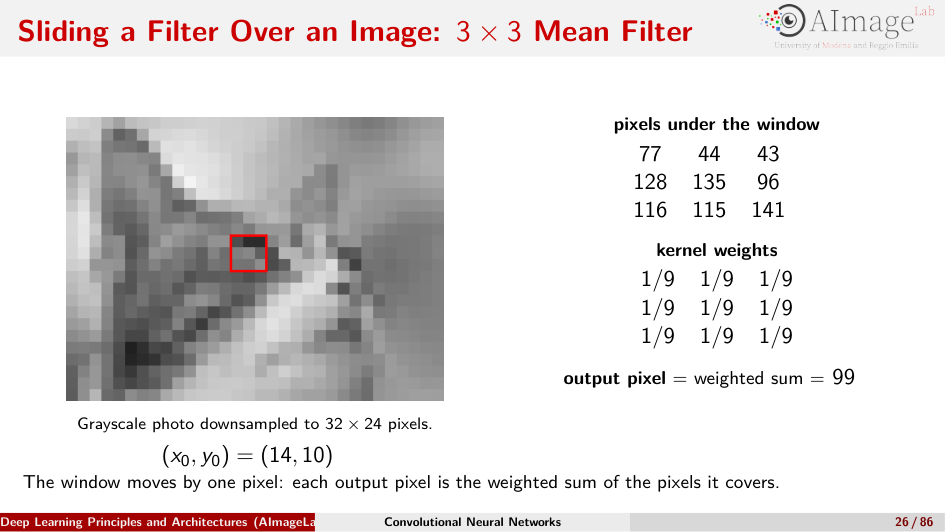
\includegraphics[keepaspectratio]{figure/fig_841268a2f8180203.png}} \pandocbounded{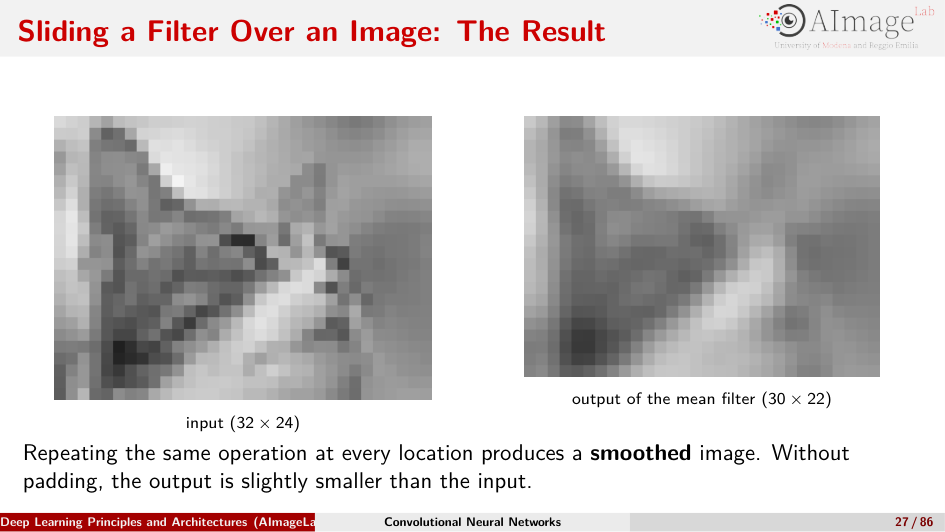
\includegraphics[keepaspectratio]{figure/fig_945718f1e47f39ff.png}}
% END F02-B0107

% BEGIN F02-B0108
Ripetendo l\textquotesingle operazione per tutte le coordinate si ottiene la mappa filtrata (Slide 31). In assenza di accorgimenti per i bordi, l\textquotesingle immagine risultante subisce una lieve riduzione di dimensioni (da \(32 \times 24\) a \(30 \times 22\)).
% END F02-B0108

% BEGIN F02-B0109
\subsection{Chiarimento Didattico: Dove Viene Collocato il Valore Calcolato?}\label{f02-r338}
% END F02-B0109

% BEGIN F02-B0110
Durante la spiegazione dell\textquotesingle operatore a finestra mobile emergono spesso dubbi sul significato dell\textquotesingle uscita e sul suo posizionamento:
% END F02-B0110

% BEGIN F02-B0111
\begin{enumerate}
\def\labelenumi{\arabic{enumi}.}
\item
  \textbf{Un filtro locale modifica l\textquotesingle immagine sovrascrivendo i pixel coperti?}\\
  No. L\textquotesingle immagine di uscita è inizialmente una matrice vuota. L\textquotesingle applicazione del kernel su un\textquotesingle intera finestra di \(3 \times 3\) pixel non produce 9 valori, bensì \textbf{un singolo valore scalare}. Questo valore viene inserito in una coordinata specifica della nuova immagine di output, mentre i pixel originali rimangono intatti per i calcoli successivi.
\item
  \textbf{In quale cella dell\textquotesingle output viene inserito lo scalare calcolato?}\\
  Dipende dalla convenzione adottata per il sistema di coordinate del filtro: La scelta del centro o dell\textquotesingle angolo superiore sinistro è una convenzione di indicizzazione. Non distingue convoluzione e correlazione: la convoluzione ribalta il kernel lungo entrambi gli assi, mentre la correlazione lo applica senza ribaltarlo. Per un kernel simmetrico i risultati coincidono. Con patch \([1,2]\) e pesi \([3,4]\), la correlazione dà \(1\cdot3+2\cdot4=11\), l\textquotesingle applicazione ribaltata dà \(1\cdot4+2\cdot3=10\). Limiti interi inclusivi da \(-3\) a \(3\) comprendono \textbf{7}, non 6, posizioni.
\item
  \textbf{Quante volte viene utilizzato ciascun pixel dell\textquotesingle input?}\\
  Un pixel interno viene condiviso e riutilizzato tante volte quante sono le posizioni del filtro che lo includono all\textquotesingle interno della propria finestra. Per un kernel \(3 \times 3\) con passo unitario, ogni pixel interno entra nel calcolo di \textbf{9 finestre distinte}, garantendo un\textquotesingle altissima ridondanza e coerenza spaziale nel segnale estratto.
\end{enumerate}
% END F02-B0111

% BEGIN F02-B0112
\subsection{Formalizzazione Matematica dell\textquotesingle Operatore LSI (slide 32--34)}\label{f02-r351}
% END F02-B0112

% BEGIN F02-B0113
Data un\textquotesingle immagine discreta di ingresso \(i(x, y)\), l\textquotesingle uscita \(o(x, y)\) prodotta da un operatore LSI \(\mathcal{T}\) con kernel discreto \(K(x, y)\) è formalmente definita da una doppia sommatoria (Slide 32):
% END F02-B0113

% BEGIN F02-B0114
\begin{center}
\begin{adjustbox}{max width=\linewidth}
$\displaystyle 
\boxed{o(x, y) = \mathcal{T}\{i\}(x, y) = \sum_{m} \sum_{n} i(m, n) \cdot K(x - m, y - n)}
$
\end{adjustbox}
\end{center}
% END F02-B0114

% BEGIN F02-B0115
dove \(K(x, y) = \mathcal{T}\{\delta\}(x, y)\) rappresenta la \textbf{risposta all\textquotesingle impulso} dell\textquotesingle operatore applicato alla delta di Kronecker bidimensionale \(\delta(x, y)\).
% END F02-B0115

% BEGIN F02-B0116
\pandocbounded{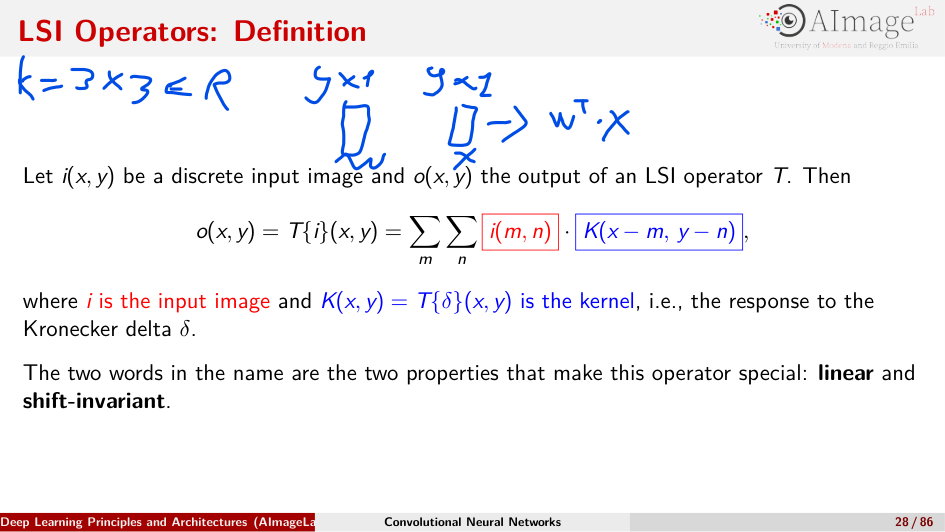
\includegraphics[keepaspectratio]{figure/fig_77cac5b1f31f104c.png}} \pandocbounded{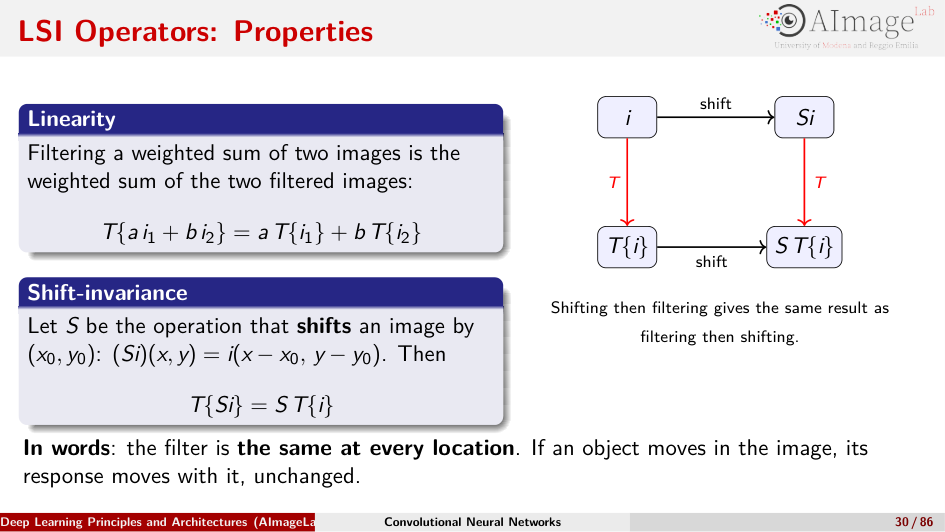
\includegraphics[keepaspectratio]{figure/fig_9bdd95a5fa59678a.png}}
% END F02-B0116

% BEGIN F02-B0117
Le due proprietà algebriche fondamentali enunciate nella Slide 34 sono:
% END F02-B0117

% BEGIN F02-B0118
\begin{enumerate}
\def\labelenumi{\arabic{enumi}.}
\tightlist
\item
  \textbf{Linearità}: \begin{center}
\begin{adjustbox}{max width=\linewidth}
$\displaystyle 
  \mathcal{T}\{a \cdot i_1 + b \cdot i_2\} = a \cdot \mathcal{T}\{i_1\} + b \cdot \mathcal{T}\{i_2\}, \quad \forall a, b \in \mathbb{R}
  $
\end{adjustbox}
\end{center}
\item
  \textbf{Invarianza alla traslazione (Shift-Invariance / Translation Equivariance)}:\\
  Sia \(S_{(x_0, y_0)}\) l\textquotesingle operatore di traslazione spaziale definito da \((S i)(x, y) = i(x - x_0, y - y_0)\). Allora: \begin{center}
\begin{adjustbox}{max width=\linewidth}
$\displaystyle 
  \boxed{\mathcal{T}\{S i\} = S \mathcal{T}\{i\}}
  $
\end{adjustbox}
\end{center}
\end{enumerate}
% END F02-B0118

% BEGIN F02-B0119
In termini discorsivi: \textbf{traslare l\textquotesingle immagine e poi applicare il filtro produce lo stesso identico risultato che applicare il filtro e successivamente traslare la mappa di uscita}.
% END F02-B0119

% BEGIN F02-B0120
\subsubsection{L\textquotesingle Intuizione Fisica: Risposta Massima e Sovrapposizione di Forme}\label{f02-r378}
% END F02-B0120

% BEGIN F02-B0121
Il significato profondo del prodotto di convoluzione tra un segnale e un kernel può essere compreso analizzando la risposta in 1D o 2D: il valore di uscita misura il grado di somiglianza locale (allineamento per prodotto scalare) tra il profilo del filtro e la porzione di segnale sottostante.
% END F02-B0121

% BEGIN F02-B0122
L'analogia delle forme a incastro aiuta a interpretare un filtro come rilevatore di pattern. Un buon allineamento può produrre una risposta alta, ma il prodotto scalare dipende anche dall'intensità e dai segni: non è una misura normalizzata di somiglianza e non genera in generale un unico impulso con zero altrove. La delta di Kronecker definisce invece l'impulso usato per identificare la risposta del sistema.
% END F02-B0122

% BEGIN F02-B0123
Se il pattern si sposta all\textquotesingle interno dell\textquotesingle immagine, la proprietà di shift-invariance garantisce che anche il picco della risposta si sposterà esattamente della medesima quantità, senza alterare la propria intensità o conformazione.
% END F02-B0123

% BEGIN F02-B0124
\begin{center}\rule{0.5\linewidth}{0.5pt}\end{center}
% END F02-B0124

% BEGIN F02-B0125
\section{Il Nucleo della Convoluzione nel Deep Learning (slide 35--39)}\label{f02-r388}
% END F02-B0125

% BEGIN F02-B0126
Il passaggio rivoluzionario dalla Computer Vision classica al Deep Learning risiede in un cambio di paradigma fondamentale (Slide 35): \textbf{i coefficienti del kernel non vengono più progettati a mano da un esperto umano, ma vengono trattati come parametri liberi da apprendere direttamente dai dati mediante Backpropagation}.
% END F02-B0126

% BEGIN F02-B0127
\begin{figure}[H]
\centering
\pandocbounded{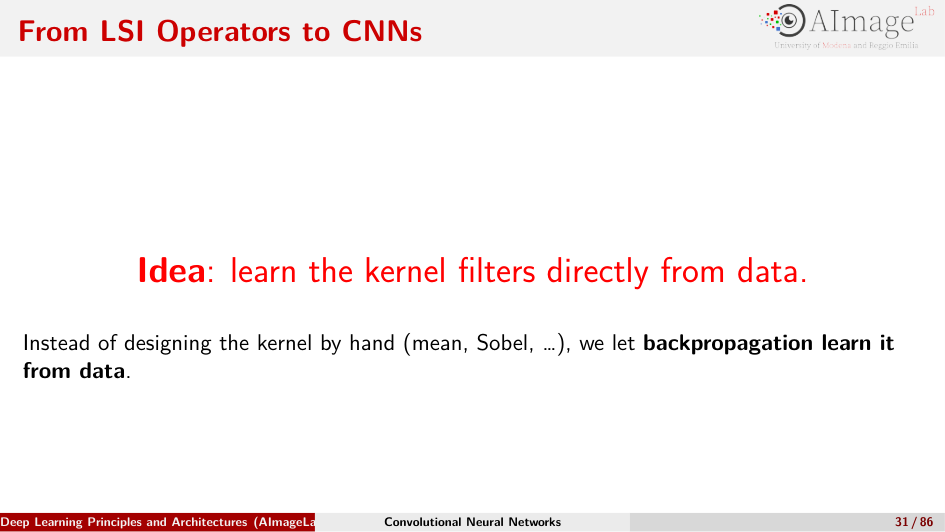
\includegraphics[keepaspectratio]{figure/fig_0d11516aaea9fd48.png}}
\caption{Slide 35 -- From LSI Operators to CNNs}
\end{figure}
% END F02-B0127

% BEGIN F02-B0128
\subsection{La Convoluzione 2D come Percettrone Locale Scorrevole (slide 36)}\label{f02-r394}
% END F02-B0128

% BEGIN F02-B0129
Si consideri l\textquotesingle operazione di filtraggio locale su una porzione di matrice \(3 \times 3\) con un filtro \(2 \times 2\) (Slide 36):
% END F02-B0129

% BEGIN F02-B0130
\begin{figure}[H]
\centering
\pandocbounded{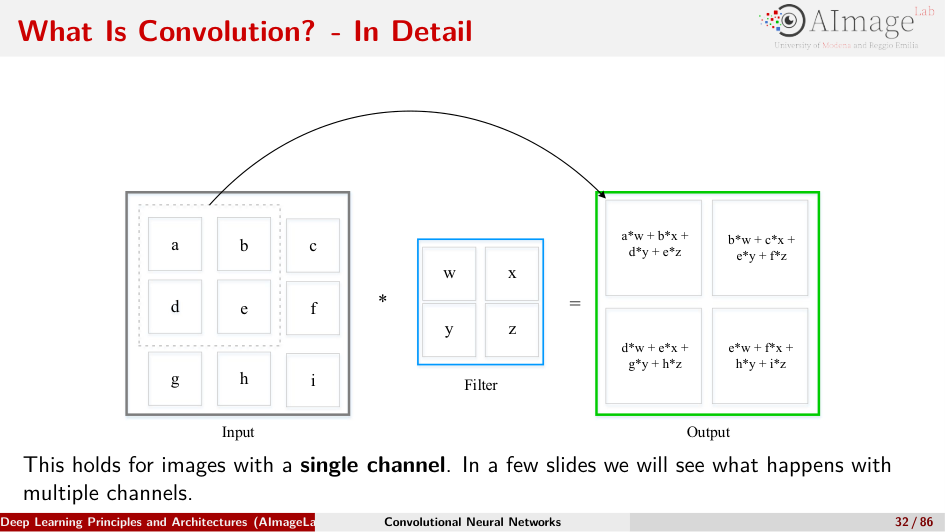
\includegraphics[keepaspectratio]{figure/fig_b00eef0a3e4b7555.png}}
\caption{Slide 36 -- What Is Convolution? - In Detail}
\end{figure}
% END F02-B0130

% BEGIN F02-B0131
\begin{center}
\begin{adjustbox}{max width=\linewidth}
$\displaystyle 
\text{Input} = \begin{bmatrix} a & b & c \\ d & e & f \\ g & h & i \end{bmatrix}, \qquad \text{Filtro} = \begin{bmatrix} w & x \\ y & z \end{bmatrix}
$
\end{adjustbox}
\end{center}
% END F02-B0131

% BEGIN F02-B0132
L\textquotesingle uscita nelle quattro posizioni spaziali è:
% END F02-B0132

% BEGIN F02-B0133
\begin{center}
\begin{adjustbox}{max width=\linewidth}
$\displaystyle 
\text{Output} = \begin{bmatrix}
a \cdot w + b \cdot x + d \cdot y + e \cdot z & b \cdot w + c \cdot x + e \cdot y + f \cdot z \\
d \cdot w + e \cdot x + g \cdot y + h \cdot z & e \cdot w + f \cdot x + h \cdot y + i \cdot z
\end{bmatrix}
$
\end{adjustbox}
\end{center}
% END F02-B0133

% BEGIN F02-B0134
Se appiattiamo i 4 coefficienti del filtro in un vettore pesi \(w = [w, x, y, z]^T \in \mathbb{R}^4\) e i 4 pixel della prima finestra locale in un vettore \(x_{(1)} = [a, b, d, e]^T \in \mathbb{R}^4\), l\textquotesingle operazione calcolata coincide con:
% END F02-B0134

% BEGIN F02-B0135
\begin{center}
\begin{adjustbox}{max width=\linewidth}
$\displaystyle 
\text{Out}_{(1, 1)} = w^T x_{(1)} + b
$
\end{adjustbox}
\end{center}
% END F02-B0135

% BEGIN F02-B0136
Questa formulazione dimostra che \textbf{un\textquotesingle operazione convoluzionale non è altro che un piccolo percettrone lineare (un micro-MLP) dotato di pochissimi pesi, che viene fatto scorrere linearmente su tutte le coordinate dell\textquotesingle immagine}.
% END F02-B0136

% BEGIN F02-B0137
\subsection{I Due Principi Fondamentali: Connettività Sparsa e Condivisione dei Pesi (slide 37--39)}\label{f02-r421}
% END F02-B0137

% BEGIN F02-B0138
Le CNN modificano radicalmente l\textquotesingle approccio dell\textquotesingle MLP densamente connesso attraverso due regole di progettazione (Slide 37):
% END F02-B0138

% BEGIN F02-B0139
\begin{figure}[H]
\centering
\pandocbounded{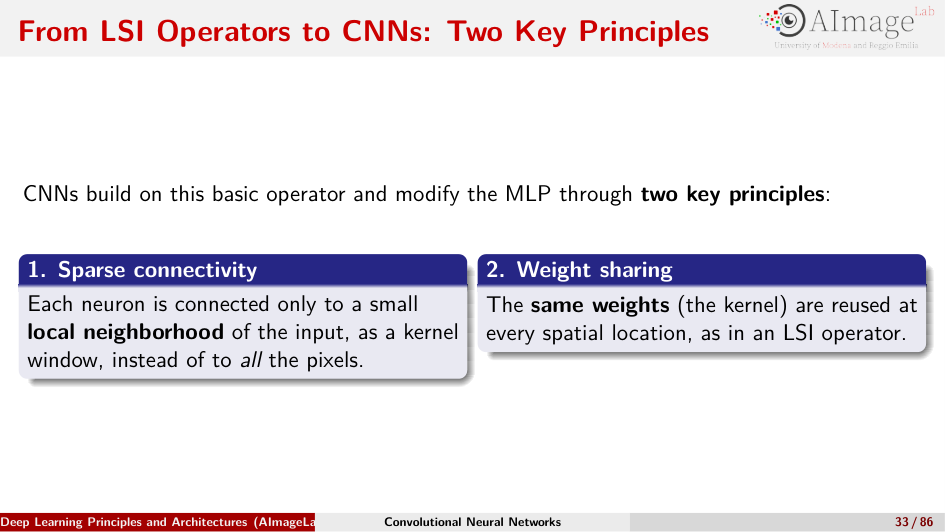
\includegraphics[keepaspectratio]{figure/fig_634e937fa66a3153.png}}
\caption{Slide 37 -- From LSI Operators to CNNs: Two Key Principles}
\end{figure}
% END F02-B0139

% BEGIN F02-B0140
\begin{enumerate}
\def\labelenumi{\arabic{enumi}.}
\tightlist
\item
  \textbf{Connettività Sparsa (Sparse Connectivity, Slide 38)}: ogni neurone dello strato convoluzionale non è connesso a tutti i pixel dell\textquotesingle immagine di ingresso, ma interagisce unicamente con una piccola regione spaziale locale e contigua. Questa regione delimitata costituisce il \textbf{Receptive Field} (campo recettivo) del neurone.
\item
  \textbf{Condivisione dei Pesi (Weight Sharing / Parameter Sharing, Slide 39)}: il medesimo insieme di coefficienti numerici (il kernel) e lo stesso termine di bias vengono riutilizzati per calcolare le risposte in \textbf{tutte} le posizioni spaziali dell\textquotesingle immagine. Tutti i neuroni che concorrono alla generazione di una specifica mappa di feature condividono identici pesi.
\end{enumerate}
% END F02-B0140

% BEGIN F02-B0141
\pandocbounded{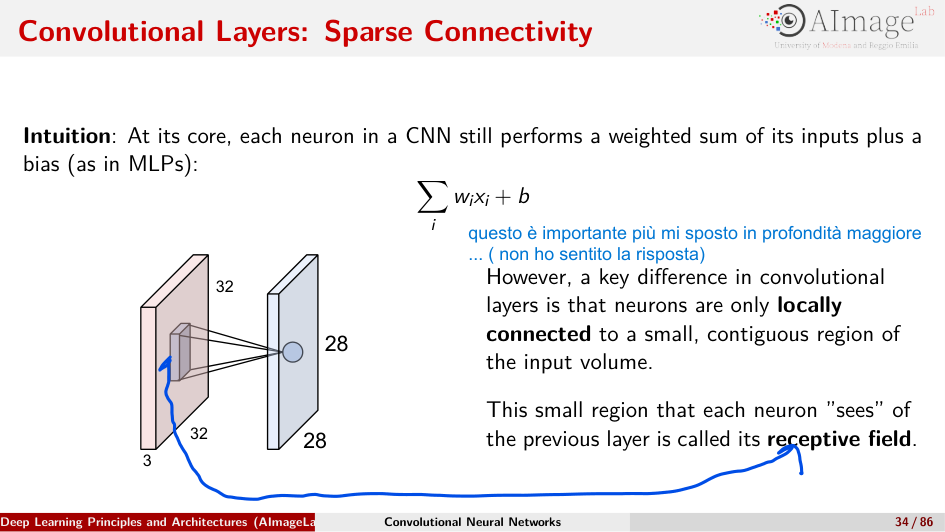
\includegraphics[keepaspectratio]{figure/fig_fcd676334826a71d.png}} \pandocbounded{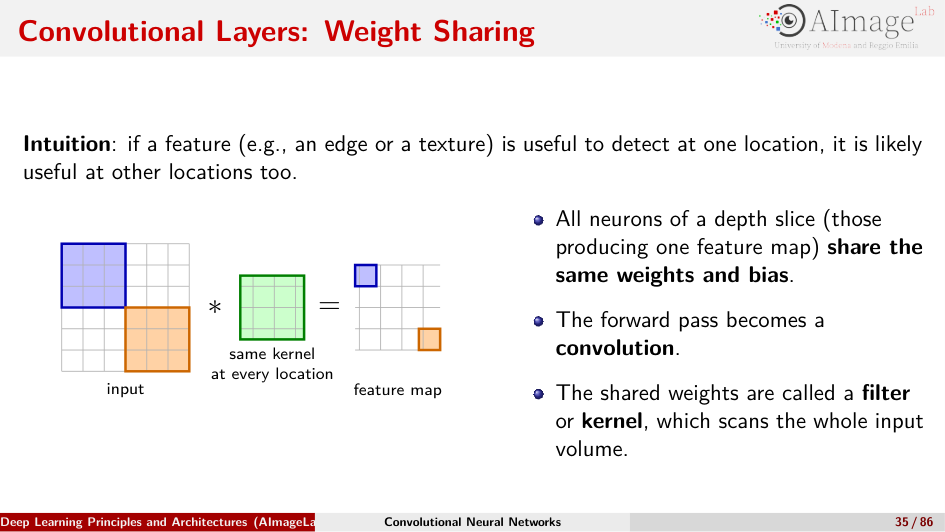
\includegraphics[keepaspectratio]{figure/fig_b0723d836b57c579.png}}
% END F02-B0141

% BEGIN F02-B0142
\subsection{Risoluzione del Punto Aperto: Il Concetto e la Crescita del Receptive Field (slide 38)}\label{f02-r433}
% END F02-B0142

% BEGIN F02-B0143
Nella slide 38 compare una riflessione didattica lasciata aperta:
% END F02-B0143

% BEGIN F02-B0144
\begin{quote}
\emph{"Questo è importante: più mi sposto in profondità, maggiore è ... "}
\end{quote}
% END F02-B0144

% BEGIN F02-B0145
La risposta analitica e concettuale è: \textbf{il Receptive Field (campo recettivo teorico) cresce progressivamente all\textquotesingle aumentare della profondità della rete}.
% END F02-B0145

% BEGIN F02-B0146
Si analizzi la meccanica di composizione su più strati successivi: * Un neurone appartenente alla prima mappa di feature possiede un campo recettivo limitato, pari all\textquotesingle estensione spaziale del primo filtro (ad esempio \(3 \times 3\) pixel dell\textquotesingle immagine di input). * Un neurone del secondo strato convoluzionale elabora una finestra \(3 \times 3\) della mappa di feature prodotta dal primo strato. Ciascuno di questi 9 elementi, a sua volta, sintetizza l\textquotesingle informazione di una propria finestra \(3 \times 3\) sull\textquotesingle immagine originaria. * Attraverso la sovrapposizione geometrica delle finestre, il singolo neurone del secondo strato "vede" indirettamente un\textquotesingle area considerevolmente più ampia dell\textquotesingle immagine originale (un patch di \(5 \times 5\) pixel). * Procedendo verso strati via via più profondi (specialmente in presenza di stride o pooling), il campo recettivo teorico si espande a ventaglio fino a coprire decine o centinaia di pixel, arrivando a comprendere l\textquotesingle intero fotogramma.
% END F02-B0146

% BEGIN F02-B0147
\pandocbounded{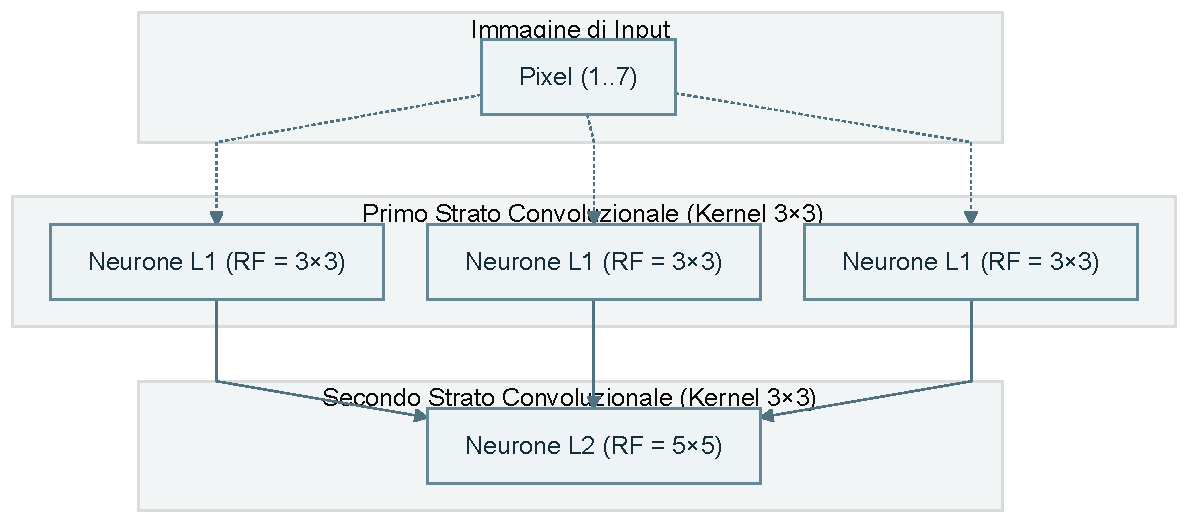
\includegraphics[keepaspectratio]{figure/diagramma_f02_04.pdf}}
% END F02-B0147

% BEGIN F02-B0148
Questa proprietà risolve un dilemma fondamentale: come può una rete neurale riconoscere oggetti di grandi dimensioni (come un\textquotesingle intera automobile o un volto umano) se i suoi filtri elementari sono minuscoli matrici \(3 \times 3\)? La risposta risiede proprio nella \textbf{crescita del campo recettivo}: non è necessario costruire filtri giganteschi (che comporterebbero troppi parametri), ma basta impilare strati con filtri piccoli per comporre gerarchicamente le informazioni locali in rappresentazioni globali.
% END F02-B0148

% BEGIN F02-B0149
\begin{center}\rule{0.5\linewidth}{0.5pt}\end{center}
% END F02-B0149

% BEGIN F02-B0150
\subsection{Crescita del campo recettivo: risposta al dubbio della slide 38}\label{f02-r473}
% END F02-B0150

% BEGIN F02-B0151
Il campo recettivo teorico è l\textquotesingle insieme delle posizioni dell\textquotesingle immagine che possono influenzare un\textquotesingle uscita. Non coincide con l\textquotesingle importanza effettiva di ciascun pixel, che dipende dai pesi. Indicando con \(r_\ell\) la sua ampiezza e con \(j_\ell\) la distanza fra due uscite adiacenti misurata sull\textquotesingle immagine iniziale, per kernel di ampiezza \(k_\ell\) e stride \(s_\ell\), senza dilatazione: \begin{center}
\begin{adjustbox}{max width=\linewidth}
$\displaystyle 
\boxed{r_\ell=r_{\ell-1}+(k_\ell-1)j_{\ell-1},\qquad j_\ell=s_\ell j_{\ell-1}.}
$
\end{adjustbox}
\end{center} Si parte da \(r_0=j_0=1\). Una finestra unisce \(k_\ell\) campi del livello precedente, i cui centri sono distanti \(j_{\ell-1}\): dal primo all\textquotesingle ultimo si aggiungono \(k_\ell-1\) intervalli. Con due convoluzioni \(3\times3\) a stride 1 si ottiene \(r_1=3\), \(r_2=5\).
% END F02-B0151

% BEGIN F02-B0152
L\textquotesingle esempio orale parte da una griglia \(4\times4\). Un kernel \(2\times2\) a stride 2 produce una griglia \(2\times2\): ogni uscita riassume quattro pixel. Un altro kernel \(2\times2\) unisce le quattro uscite in un solo valore: \(r_2=2+(2-1)\cdot2=4\), quindi può dipendere dall\textquotesingle intera immagine. Si compongono pattern piccoli in pattern estesi senza apprendere fin dall\textquotesingle inizio un filtro grande quanto l\textquotesingle immagine. Non si può concludere che un filtro grande diretto sia più preciso: i modelli hanno parametrizzazioni differenti e, con attivazioni intermedie, non sono equivalenti.
% END F02-B0152

% BEGIN F02-B0153
\section{Convoluzione Multicanale e Feature Maps (slide 40--42)}\label{f02-r483}
% END F02-B0153

% BEGIN F02-B0154
Nelle applicazioni reali le immagini di ingresso non sono scalari monodimensionali (possiedono \(C_{in} = 3\) canali cromatici RGB), e gli strati intermedi operano su volumi composti da decine o centinaia di canali di feature.
% END F02-B0154

% BEGIN F02-B0155
\subsection{\texorpdfstring{Il Filtro Tridimensionale (\(C_{in} > 1\), slide 40)}{Il Filtro Tridimensionale (C\_\{in\} \textgreater{} 1, slide 40)}}\label{f02-r487}
% END F02-B0155

% BEGIN F02-B0156
Quando il volume di ingresso ha forma \(H \times W \times C_{in}\), un filtro convoluzionale \textbf{non è una matrice bidimensionale, bensì un volume tridimensionale (un parallelepipedo parametrico)} di dimensioni:
% END F02-B0156

% BEGIN F02-B0157
\begin{center}
\begin{adjustbox}{max width=\linewidth}
$\displaystyle 
\boxed{K \times K \times C_{in}}
$
\end{adjustbox}
\end{center}
% END F02-B0157

% BEGIN F02-B0158
Il filtro si estende per l\textquotesingle intera profondità dei canali di ingresso. Esso è composto da una pila di \(C_{in}\) fette bidimensionali distinte di parametri, ciascuna di dimensione \(K \times K\):
% END F02-B0158

% BEGIN F02-B0159
\begin{center}
\begin{adjustbox}{max width=\linewidth}
$\displaystyle 
(K_1, K_2, \dots, K_{C_{in}})
$
\end{adjustbox}
\end{center}
% END F02-B0159

% BEGIN F02-B0160
\begin{figure}[H]
\centering
\pandocbounded{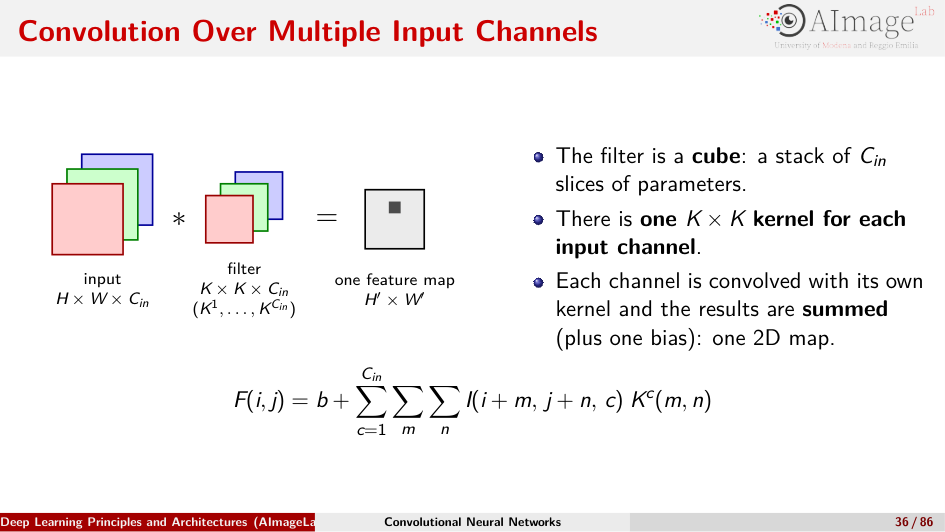
\includegraphics[keepaspectratio]{figure/fig_6266defdbcc45253.png}}
\caption{Slide 40 -- Convolution Over Multiple Input Channels}
\end{figure}
% END F02-B0160

% BEGIN F02-B0161
La formula formale per il calcolo del valore nella mappa di feature \(F(i, j)\) alla coordinata spaziale \((i, j)\) è (Slide 40):
% END F02-B0161

% BEGIN F02-B0162
\begin{center}
\begin{adjustbox}{max width=\linewidth}
$\displaystyle 
\boxed{F(i, j) = b + \sum_{c=1}^{C_{in}} \sum_{m} \sum_{n} I(i + m, j + n, c) \cdot K_c(m, n)}
$
\end{adjustbox}
\end{center}
% END F02-B0162

% BEGIN F02-B0163
dove \(I(i+m, j+n, c)\) denota il pixel dell\textquotesingle input nel canale \(c\), \(K_c(m, n)\) rappresenta il peso corrispondente nella fetta \(c\) del filtro, e \(b \in \mathbb{R}\) è l\textquotesingle unico termine scalare di bias associato al filtro.
% END F02-B0163

% BEGIN F02-B0164
Il calcolo procede dunque secondo tre passi: 1. Si calcola la convoluzione 2D tra il canale di ingresso \(c\) e la rispettiva fetta di kernel \(K_c\). 2. Si sommano i contributi scalari ottenuti attraverso \textbf{tutti} i \(C_{in}\) canali di ingresso. 3. Si aggiunge il bias scalare \(b\).
% END F02-B0164

% BEGIN F02-B0165
Il risultato dell\textquotesingle applicazione di questo filtro tridimensionale \(K \times K \times C_{in}\) è \textbf{una e una sola mappa di feature bidimensionale} di dimensioni \(H' \times W'\).
% END F02-B0165

% BEGIN F02-B0166
\subsection{\texorpdfstring{Generazione di Più Canali di Uscita (\(C_{out} > 1\), slide 41)}{Generazione di Più Canali di Uscita (C\_\{out\} \textgreater{} 1, slide 41)}}\label{f02-r518}
% END F02-B0166

% BEGIN F02-B0167
Se un singolo filtro tridimensionale produce sempre un\textquotesingle unica mappa 2D, come è possibile espandere la profondità del tensore (ad esempio trasformare un ingresso \(32 \times 32 \times 3\) in un volume \(32 \times 32 \times 32\), come visto nella Slide 22)?
% END F02-B0167

% BEGIN F02-B0168
A questo proposito è utile richiamare una metafora didattica efficace: se un pescatore prende una trota ogni volta che getta la canna da pesca, per ottenere 32 trote non può pretendere che una sola canna catturi magicamente 32 pesci insieme: deve compiere l\textquotesingle azione di pesca 32 volte distinte.
% END F02-B0168

% BEGIN F02-B0169
Allo stesso modo, \textbf{per ottenere \(C_{out}\) mappe di feature distinte dobbiamo applicare \(C_{out}\) filtri tridimensionali indipendenti}:
% END F02-B0169

% BEGIN F02-B0170
\begin{figure}[H]
\centering
\pandocbounded{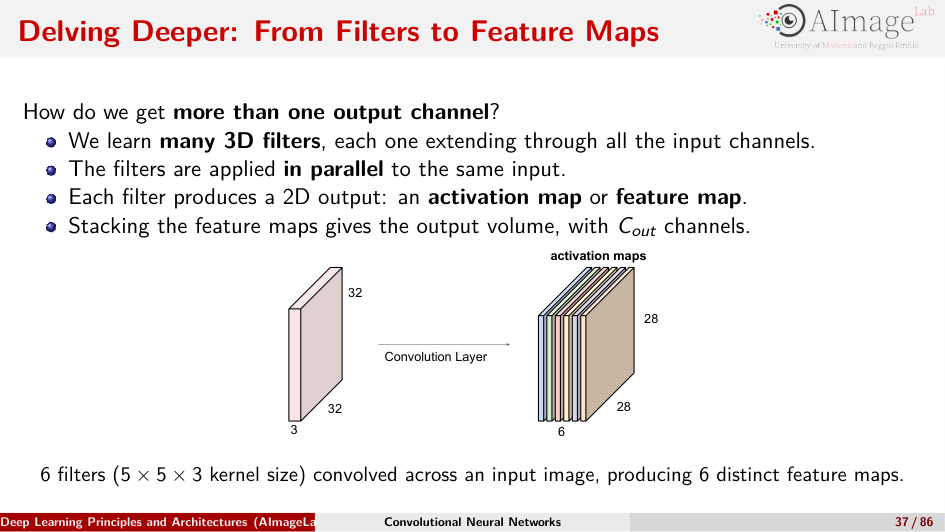
\includegraphics[keepaspectratio]{figure/fig_65b2598d36400200.png}}
\caption{Slide 41 -- Delving Deeper: From Filters to Feature Maps}
\end{figure}
% END F02-B0170

% BEGIN F02-B0171
Ciascuno dei \(C_{out}\) filtri possiede un proprio set esclusivo di pesi di dimensione \(K \times K \times C_{in}\) e un proprio bias \(b_k\). Ciascun filtro scorre sull\textquotesingle intero volume di ingresso e genera la propria mappa bidimensionale \(H' \times W'\). Impilando (\emph{stacking}) le \(C_{out}\) mappe di attivazione lungo l\textquotesingle asse della profondità si ottiene il volume di uscita:
% END F02-B0171

% BEGIN F02-B0172
\begin{center}
\begin{adjustbox}{max width=\linewidth}
$\displaystyle 
\boxed{Y \in \mathbb{R}^{H' \times W' \times C_{out}}}
$
\end{adjustbox}
\end{center}
% END F02-B0172

% BEGIN F02-B0173
Ad esempio, nell\textquotesingle illustrazione della Slide 41: * Ingresso: \(32 \times 32 \times 3\) (\(C_{in} = 3\)). * Strato convoluzionale: \(C_{out} = 6\) filtri indipendenti di dimensione \(5 \times 5 \times 3\). * Uscita: volume di 6 mappe di feature di dimensione \(28 \times 28\), ovvero forma complessiva \(28 \times 28 \times 6\).
% END F02-B0173

% BEGIN F02-B0174
\begin{center}\rule{0.5\linewidth}{0.5pt}\end{center}
% END F02-B0174

% BEGIN F02-B0175
\section{Iperparametri del Livello Convoluzionale: Kernel, Stride e Padding (slide 43--46)}\label{f02-r541}
% END F02-B0175

% BEGIN F02-B0176
La configurazione operativa di uno strato convoluzionale è governata da quattro iperparametri cardinali (Slide 43--44):
% END F02-B0176

% BEGIN F02-B0177
\begin{enumerate}
\def\labelenumi{\arabic{enumi}.}
\tightlist
\item
  \textbf{Numero di filtri (\(C_{out}\))}: determina la profondità del volume di uscita, ovvero quante feature maps distinte vengono estratte in parallelo.
\item
  \textbf{Dimensione spaziale del kernel (\(K \times K\))}: l\textquotesingle ampiezza geometrica del campo di vista locale dei filtri (generalmente quadrati e dispari: \(3 \times 3\), \(5 \times 5\), \(7 \times 7\)). La terza dimensione coincide per definizione con il numero di canali di ingresso \(C_{in}\).
\item
  \textbf{Passo di scorrimento (Stride \(S\))}: il numero di pixel di cui la finestra del filtro si sposta a ogni passo lungo l\textquotesingle asse orizzontale e verticale.
\item
  \textbf{Padding spaziale (\(P\))}: il numero di pixel fittizi aggiunti attorno al perimetro dell\textquotesingle immagine di ingresso.
\end{enumerate}
% END F02-B0177

% BEGIN F02-B0178
\begin{figure}[H]
\centering
\pandocbounded{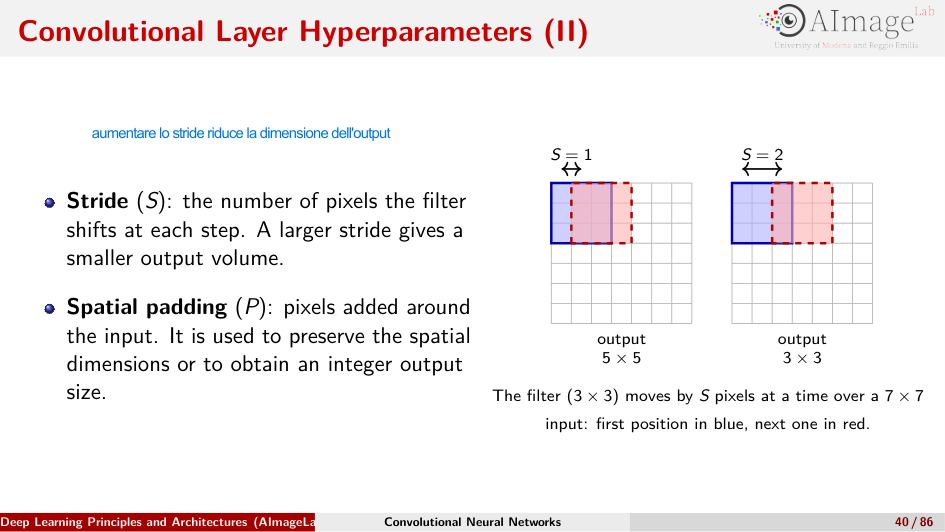
\includegraphics[keepaspectratio]{figure/fig_14c48838a6c748f3.png}}
\caption{Slide 44 -- Convolutional Layer Hyperparameters (II)}
\end{figure}
% END F02-B0178

% BEGIN F02-B0179
\subsection{\texorpdfstring{L\textquotesingle Effetto dello Stride (\(S\))}{L\textquotesingle Effetto dello Stride (S)}}\label{f02-r552}
% END F02-B0179

% BEGIN F02-B0180
\begin{itemize}
\tightlist
\item
  Con \textbf{\(S = 1\)}, il filtro trasla di una singola unità di pixel adiacente alla volta, scandendo capillarmente ogni coordinata.
\item
  Con \textbf{\(S > 1\)} (tipicamente \(S = 2\)), il filtro salta pixel intermedi. L\textquotesingle effetto immediato è una decisa riduzione spaziale delle dimensioni della mappa prodotta (un sottocampionamento diretto): con \(S = 2\) le dimensioni spaziali dell\textquotesingle uscita risultano approssimativamente dimezzate rispetto all\textquotesingle ingresso.
\end{itemize}
% END F02-B0180

% BEGIN F02-B0181
La Slide 44 mostra un input \(7 \times 7\) elaborato con filtro \(3 \times 3\): * Con \(S = 1\) e nessun padding: il filtro trasla di 1 pixel producendo una griglia \(5 \times 5\). * Con \(S = 2\) e nessun padding: il filtro compie salti di 2 pixel (posizioni alle coordinate 1, 3, 5), generando una mappa ridotta \(3 \times 3\).
% END F02-B0181

% BEGIN F02-B0182
\subsection{\texorpdfstring{Il Fenomeno dell\textquotesingle Erosione dei Bordi e il Ruolo del Padding (\(P\))}{Il Fenomeno dell\textquotesingle Erosione dei Bordi e il Ruolo del Padding (P)}}\label{f02-r561}
% END F02-B0182

% BEGIN F02-B0183
Quando un kernel di ampiezza \(K \times K\) scorre su un\textquotesingle immagine senza uscire dai bordi, le coordinate periferiche non dispongono di un numero sufficiente di vicini per centrare il filtro. Questo comporta due gravi inconvenienti: 1. \textbf{Erosione spaziale (\emph{Border eating phenomenon})}: a ogni strato convoluzionale privo di padding le dimensioni dell\textquotesingle immagine si restringono forzatamente. In reti profonde con decine di livelli, le dimensioni spaziali collasserebbero a \(1 \times 1\) dopo pochissimi strati. 2. \textbf{Sotto-rappresentazione dei bordi}: i pixel situati sugli angoli e lungo le cornici dell\textquotesingle immagine vengono inclusi in un numero di finestre molto inferiore rispetto ai pixel centrali, subendo una perdita ingiustificata di informazione.
% END F02-B0183

% BEGIN F02-B0184
Per ovviare a questo problema si introduce il \textbf{Padding (\(P\))}, ovvero una cornice di pixel sintetici aggiunta attorno all\textquotesingle immagine prima del filtraggio (Slide 45--46).
% END F02-B0184

% BEGIN F02-B0185
\begin{figure}[H]
\centering
\pandocbounded{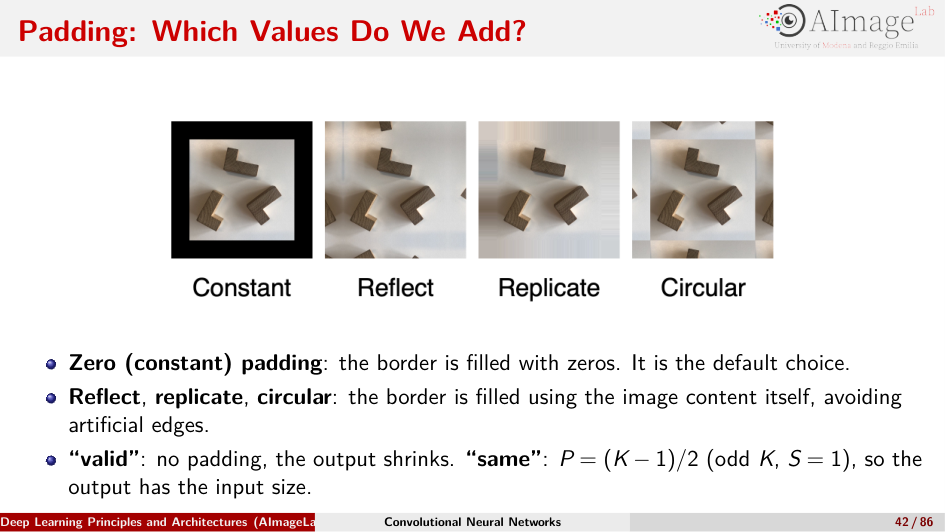
\includegraphics[keepaspectratio]{figure/fig_4bbe8f808d039366.png}}
\caption{Slide 46 -- Padding: Which Values Do We Add?}
\end{figure}
% END F02-B0185

% BEGIN F02-B0186
Le modalità principali di padding sono: * \textbf{Zero Padding (Constant Padding)}: i pixel di bordo vengono impostati a zero. Rappresenta la scelta di gran lunga prevalente e predefinita nel Deep Learning per via della sua semplicità computazionale. * \textbf{Reflect Padding}: i valori di bordo vengono riempiti specchiando specularmente i pixel interni verso l\textquotesingle esterno, attenuando la formazione di discontinuità artificiali ad alto contrasto sui bordi. * \textbf{Replicate Padding}: copia e ripete l\textquotesingle ultimo valore valido di riga o colonna fino al limite del bordo. * \textbf{Circular Padding}: assume una topologia toroidale periodica, ricopiando il margine opposto dell\textquotesingle immagine.
% END F02-B0186

% BEGIN F02-B0187
\subsubsection{Le Convenzioni "Valid" e "Same"}\label{f02-r577}
% END F02-B0187

% BEGIN F02-B0188
\begin{itemize}
\tightlist
\item
  \textbf{Padding "valid"}: corrisponde a \(P = 0\). Il filtro elabora unicamente posizioni in cui è interamente contenuto nell\textquotesingle immagine originaria; la mappa di uscita risulta più piccola dell\textquotesingle ingresso.
\item
  \textbf{Padding "same"}: dimensiona \(P\) in modo tale che, impostando uno stride unitario (\(S = 1\)), \textbf{le dimensioni spaziali della mappa di uscita siano esattamente identiche a quelle dell\textquotesingle ingresso} (\(H' = H, W' = W\)). Per un kernel quadrato di lato dispari \(K\), la quantità di padding necessaria per ciascun lato è determinata analiticamente da:
\end{itemize}
% END F02-B0188

% BEGIN F02-B0189
\begin{center}
\begin{adjustbox}{max width=\linewidth}
$\displaystyle 
\boxed{P = \frac{K - 1}{2}}
$
\end{adjustbox}
\end{center}
% END F02-B0189

% BEGIN F02-B0190
\begin{itemize}
\tightlist
\item
  Per kernel \(3 \times 3 \implies P = \frac{3 - 1}{2} = 1\) pixel di zero-padding su tutti e quattro i lati.
\item
  Per kernel \(5 \times 5 \implies P = \frac{5 - 1}{2} = 2\) pixel di padding per lato.
\item
  Per kernel \(7 \times 7 \implies P = \frac{7 - 1}{2} = 3\) pixel di padding per lato.
\end{itemize}
% END F02-B0190

% BEGIN F02-B0191
\subsection{Formula Universale per le Dimensioni dell\textquotesingle Uscita}\label{f02-r590}
% END F02-B0191

% BEGIN F02-B0192
Dato un volume di ingresso di dimensioni spaziali \(H \times W\), elaborato con kernel \(K \times K\), padding simmetrico \(P\) e stride \(S\), le dimensioni della mappa di feature di uscita \((H', W')\) sono rigorosamente date da:
% END F02-B0192

% BEGIN F02-B0193
\begin{center}
\begin{adjustbox}{max width=\linewidth}
$\displaystyle 
\boxed{H' = \left\lfloor \frac{H - K + 2P}{S} \right\rfloor + 1, \qquad W' = \left\lfloor \frac{W - K + 2P}{S} \right\rfloor + 1}
$
\end{adjustbox}
\end{center}
% END F02-B0193

% BEGIN F02-B0194
dove \(\lfloor \cdot \rfloor\) denota la funzione parte intera inferiore (\emph{floor}).
% END F02-B0194

% BEGIN F02-B0195
\textbf{Verifiche analitiche:} 1. \emph{Esempio Slide 41:} Input \(32 \times 32\), kernel \(5 \times 5\), \(P = 0\), \(S = 1\): \begin{center}
\begin{adjustbox}{max width=\linewidth}
$\displaystyle 
   H' = \frac{32 - 5 + 0}{1} + 1 = 27 + 1 = 28 \implies \mathbf{28 \times 28}
   $
\end{adjustbox}
\end{center} 2. \emph{Esempio Slide 44 (S=1):} Input \(7 \times 7\), kernel \(3 \times 3\), \(P = 0\), \(S = 1\): \begin{center}
\begin{adjustbox}{max width=\linewidth}
$\displaystyle 
   H' = \frac{7 - 3 + 0}{1} + 1 = 4 + 1 = 5 \implies \mathbf{5 \times 5}
   $
\end{adjustbox}
\end{center} 3. \emph{Esempio Slide 44 (S=2):} Input \(7 \times 7\), kernel \(3 \times 3\), \(P = 0\), \(S = 2\): \begin{center}
\begin{adjustbox}{max width=\linewidth}
$\displaystyle 
   H' = \left\lfloor \frac{7 - 3 + 0}{2} \right\rfloor + 1 = \frac{4}{2} + 1 = 3 \implies \mathbf{3 \times 3}
   $
\end{adjustbox}
\end{center}
% END F02-B0195

% BEGIN F02-B0196
\begin{center}\rule{0.5\linewidth}{0.5pt}\end{center}
% END F02-B0196

% BEGIN F02-B0197
Per ricavare la dimensione dell\textquotesingle uscita, si considera una sola direzione: l\textquotesingle input con padding ha \(H+2P\) posizioni. Una finestra di ampiezza \(K\) che parte in \(qS\) entra interamente se \(qS+K\leq H+2P\). Il massimo indice è \(q_{\max}=\lfloor(H+2P-K)/S\rfloor\); contando anche l\textquotesingle indice zero si ottiene \(H'=q_{\max}+1\). La stessa derivazione vale per la larghezza. Occorre che la finestra sia compatibile con l\textquotesingle input padded; si assume dilatazione 1.
% END F02-B0197

% BEGIN F02-B0198
\section{Calcolo dei Parametri Apprendibili (slide 47)}\label{f02-r618}
% END F02-B0198

% BEGIN F02-B0199
L\textquotesingle estrema efficienza delle reti convoluzionali rispetto agli strati densamente connessi emerge con evidenza dal calcolo formale dei parametri apprendibili di uno strato convoluzionale (Slide 47).
% END F02-B0199

% BEGIN F02-B0200
\begin{figure}[H]
\centering
\pandocbounded{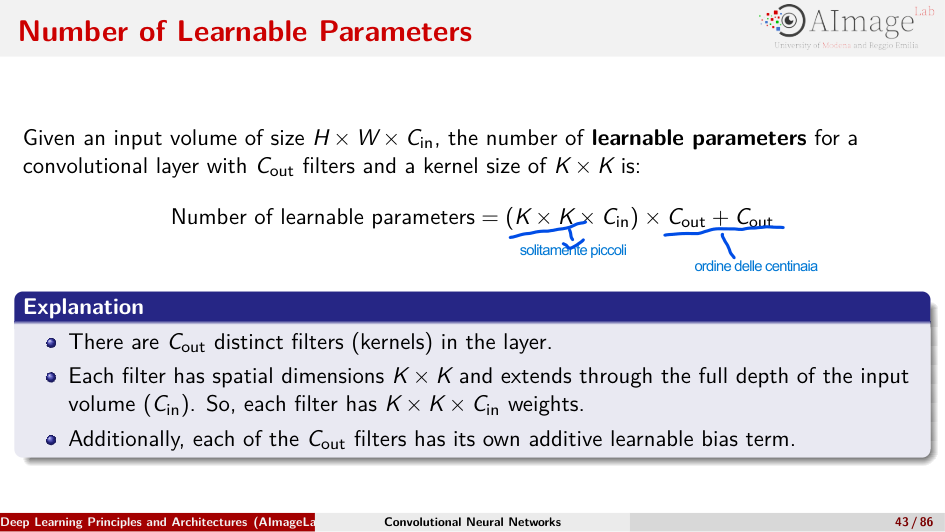
\includegraphics[keepaspectratio]{figure/fig_afd3fc828762fcef.png}}
\caption{Slide 47 -- Number of Learnable Parameters}
\end{figure}
% END F02-B0200

% BEGIN F02-B0201
Dato un volume di ingresso di forma \(H \times W \times C_{in}\) e uno strato convoluzionale definito da \(C_{out}\) filtri di dimensione \(K \times K\), il numero totale di parametri apprendibili è:
% END F02-B0201

% BEGIN F02-B0202
\begin{center}
\begin{adjustbox}{max width=\linewidth}
$\displaystyle 
\boxed{\text{Parametri} = (K \times K \times C_{in}) \times C_{out} + C_{out} = C_{out} \cdot (K^2 \cdot C_{in} + 1)}
$
\end{adjustbox}
\end{center}
% END F02-B0202

% BEGIN F02-B0203
\subsection{Dimostrazione e Scomposizione}\label{f02-r630}
% END F02-B0203

% BEGIN F02-B0204
\begin{enumerate}
\def\labelenumi{\arabic{enumi}.}
\tightlist
\item
  Ciascun filtro tridimensionale possiede dimensione spaziale \(K \times K\) ed estensione in profondità pari a \(C_{in}\). Il numero di coefficienti moltiplicativi (pesi) per ogni singolo filtro è quindi: \begin{center}
\begin{adjustbox}{max width=\linewidth}
$\displaystyle 
  \text{Pesi per filtro} = K \times K \times C_{in}
  $
\end{adjustbox}
\end{center}
\item
  Essendo presenti \(C_{out}\) filtri distinti, il numero complessivo di pesi moltiplicativi ammonta a: \begin{center}
\begin{adjustbox}{max width=\linewidth}
$\displaystyle 
  (K \times K \times C_{in}) \times C_{out}
  $
\end{adjustbox}
\end{center}
\item
  Ciascuno dei \(C_{out}\) filtri dispone di un proprio termine di \textbf{bias additivo scalare} \(b_k \in \mathbb{R}\), condiviso su tutte le coordinate della mappa \(H' \times W'\). Si hanno pertanto esattamente \(C_{out}\) bias apprendibili.
\item
  Sommando pesi e bias si ottiene la formula finale.
\end{enumerate}
% END F02-B0204

% BEGIN F02-B0205
\subsection{Il Risultato Chiave: Indipendenza dalla Risoluzione dell\textquotesingle Immagine}\label{f02-r643}
% END F02-B0205

% BEGIN F02-B0206
La proprietà teorica e computazionale più straordinaria di questa formula è che \textbf{il numero di parametri apprendibili di uno strato convoluzionale è totalmente indipendente dalle dimensioni spaziali dell\textquotesingle immagine (\(H\) e \(W\))}.
% END F02-B0206

% BEGIN F02-B0207
Si consideri un livello convoluzionale con filtri standard \(3 \times 3\), \(C_{in} = 32\) canali in ingresso e \(C_{out} = 64\) filtri in uscita:
% END F02-B0207

% BEGIN F02-B0208
\begin{center}
\begin{adjustbox}{max width=\linewidth}
$\displaystyle 
\text{Parametri} = (3 \times 3 \times 32) \times 64 + 64 = 288 \times 64 + 64 = 18.432 + 64 = \mathbf{18.496}
$
\end{adjustbox}
\end{center}
% END F02-B0208

% BEGIN F02-B0209
Che l\textquotesingle immagine di ingresso misuri \(32 \times 32\) pixel, oppure \(1000 \times 1000\) pixel, il numero di parametri liberi dello strato rimane rigorosamente \textbf{18.496} (nell\textquotesingle ordine delle decine di migliaia). Al contrario, come dimostrato nella Sezione \ref{f02-r170}, un MLP per immagini da \(1000 \times 1000\) pixel richiederebbe centinaia di milioni o miliardi di parametri. L\textquotesingle aumento della risoluzione dell\textquotesingle immagine incrementa il numero di operazioni aritmetiche nel forward pass, ma \textbf{non modifica il numero di pesi di quel livello}; non permette però di concludere che il rischio di overfitting dell'intero modello resti invariato.
% END F02-B0209

% BEGIN F02-B0210
\begin{center}\rule{0.5\linewidth}{0.5pt}\end{center}
% END F02-B0210

% BEGIN F02-B0211
\section{Visualizzazione dei Filtri e Gerarchia delle Rappresentazioni (slide 48--51)}\label{f02-r657}
% END F02-B0211

% BEGIN F02-B0212
Uno dei contributi scientifici più rilevanti dell\textquotesingle architettura \textbf{AlexNet} (Krizhevsky et al., 2012) è consistito nella possibilità di ispezionare visivamente i parametri appresi dal primo strato convoluzionale.
% END F02-B0212

% BEGIN F02-B0213
\pandocbounded{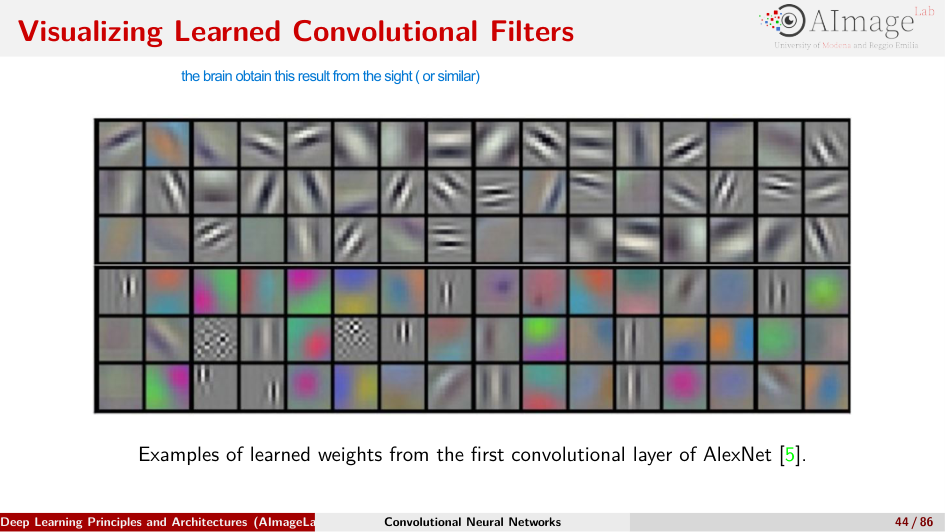
\includegraphics[keepaspectratio]{figure/fig_f416645b624d9f00.png}} \pandocbounded{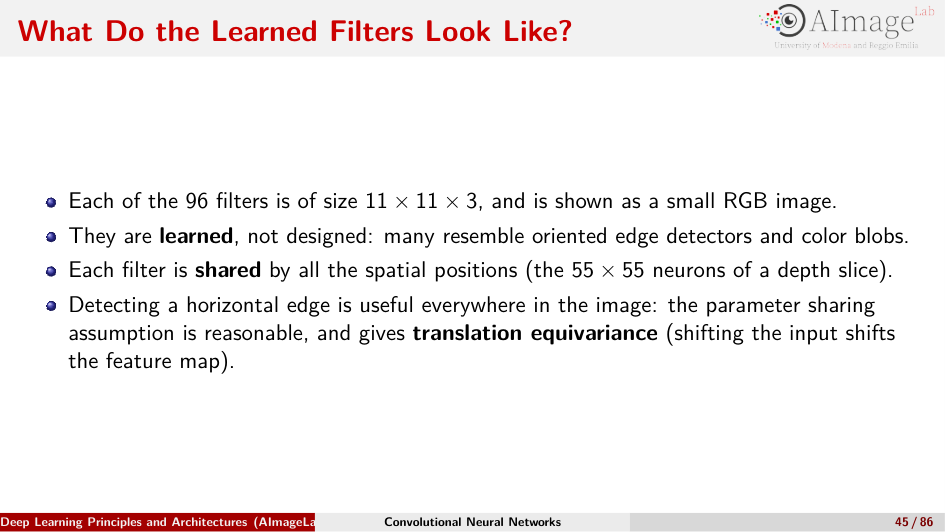
\includegraphics[keepaspectratio]{figure/fig_a6d4306da3563700.png}}
% END F02-B0213

% BEGIN F02-B0214
Il primo strato di AlexNet riceveva immagini RGB (\(C_{in} = 3\)) ed era composto da \(C_{out} = 96\) filtri con dimensione \(11 \times 11\). Poiché ciascun filtro ha dimensione \(11 \times 11 \times 3\), esso può essere direttamente convertito e renderizzato come una minuscola immagine a colori di \(11 \times 11\) pixel (Slide 49).
% END F02-B0214

% BEGIN F02-B0215
L\textquotesingle ispezione dei 96 filtri svela pattern regolari e significativi: * Molti filtri apprendono risposte a \textbf{bordi orientati (oriented edge detectors)} ad angolazioni specifiche (orizzontali, verticali, diagonali), con bande alternate di luce e buio. * Altri filtri mostrano selettività cromatica, manifestando gradienti netti o chiazze di colore opposte (\emph{color blobs}, ad esempio transizioni dal rosso al ciano o dal giallo al blu). * Altri ancora assomigliano a filtri di Gabor su diverse frequenze spaziali.
% END F02-B0215

% BEGIN F02-B0216
I filtri visualizzati emergono dall'addestramento: alcuni rilevano bordi orientati, contrasti di colore o texture. L'analogia con la visione biologica è qualitativa e non dimostra identità dei meccanismi.
% END F02-B0216

% BEGIN F02-B0217
\subsubsection{\texorpdfstring{Forma vs Texture (\emph{Shape over Texture})}{Forma vs Texture (Shape over Texture)}}\label{f02-r673}
% END F02-B0217

% BEGIN F02-B0218
Bordi, forme e texture possono contribuire al riconoscimento. Le visualizzazioni mostrano feature locali utili, ma non stabiliscono una priorità universale della forma sulla texture: il risultato dipende dal compito e dall'addestramento.
% END F02-B0218

% BEGIN F02-B0219
\subsection{Le Mappe di Attivazione (Activation Maps, slide 50)}\label{f02-r677}
% END F02-B0219

% BEGIN F02-B0220
Mentre i filtri rappresentano i parametri statici appresi dalla rete, le \textbf{mappe di attivazione (Activation Maps)} rappresentano le risposte dinamiche dei neuroni a una specifica immagine di ingresso.
% END F02-B0220

% BEGIN F02-B0221
\begin{figure}[H]
\centering
\pandocbounded{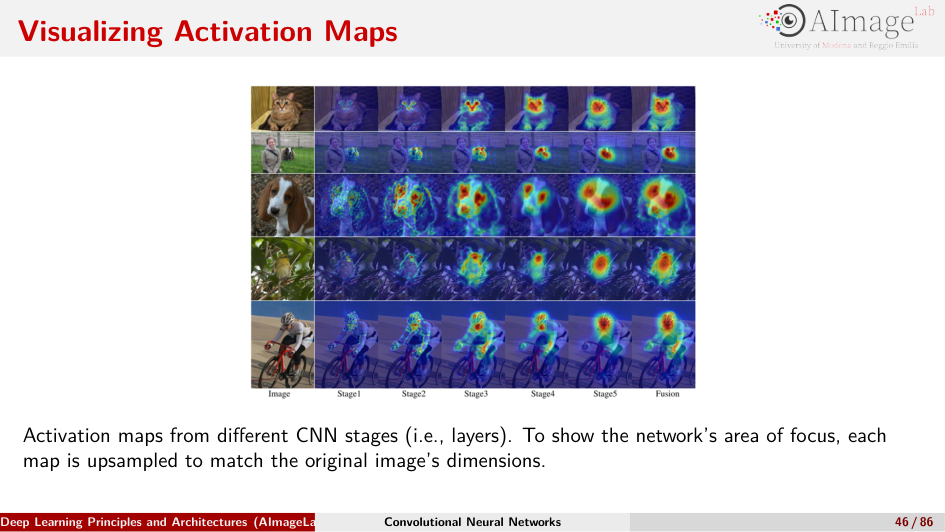
\includegraphics[keepaspectratio]{figure/fig_6c2af1f43f562e1b.png}}
\caption{Slide 50 -- Visualizing Activation Maps}
\end{figure}
% END F02-B0221

% BEGIN F02-B0222
Come mostrato nella Slide 50 (in cui le mappe vengono ricampionate alle dimensioni dell\textquotesingle immagine originale per renderle interpretabili): * Nei primi strati, le mappe si accendono in corrispondenza di singoli pixel o linee sottili che presentano l\textquotesingle orientamento o il colore ricercato dal filtro. * Negli strati intermedi e profondi, le mappe di attivazione non rispondono più a singoli pixel, ma si concentrano su intere regioni coerenti della scena (il muso di un animale, le ruote di un veicolo, una figura umana), evidenziando le aree semantiche su cui la rete focalizza la propria attenzione decisionale.
% END F02-B0222

% BEGIN F02-B0223
\subsection{La Gerarchia dei Concetti e il Transfer Learning (slide 51)}\label{f02-r687}
% END F02-B0223

% BEGIN F02-B0224
L\textquotesingle impilamento sequenziale di strati convoluzionali realizza una transizione graduale dal segnale grezzo all\textquotesingle astrazione semantica (Slide 51):
% END F02-B0224

% BEGIN F02-B0225
\begin{figure}[H]
\centering
\pandocbounded{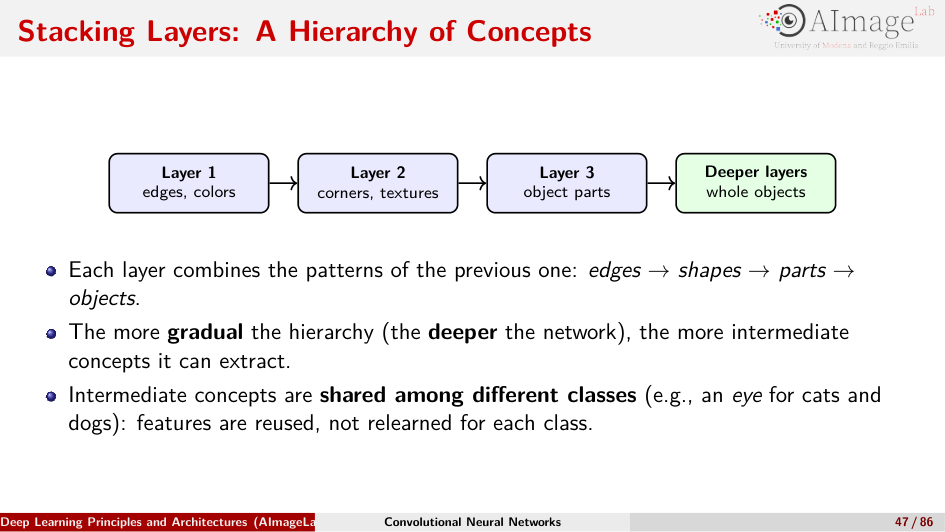
\includegraphics[keepaspectratio]{figure/fig_895e1872a6f60602.png}}
\caption{Slide 51 -- Stacking Layers: A Hierarchy of Concepts}
\end{figure}
% END F02-B0225

% BEGIN F02-B0226
\pandocbounded{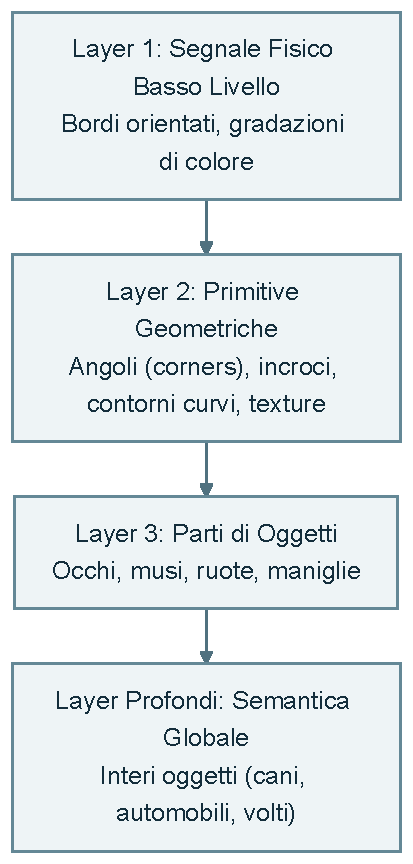
\includegraphics[keepaspectratio]{figure/diagramma_f02_05.pdf}}
% END F02-B0226

% BEGIN F02-B0227
\begin{enumerate}
\def\labelenumi{\arabic{enumi}.}
\tightlist
\item
  \textbf{Strato 1}: rileva bordi, linee e variazioni elementari di contrasto.
\item
  \textbf{Strato 2}: combina linearmente i bordi intercettando angoli (\emph{corners}), incroci a T, archi e trame tessili.
\item
  \textbf{Strato 3}: combina le forme geometriche per assemblare parti anatomiche o meccaniche riconoscibili (occhi, nasi, ruote di automobile).
\item
  \textbf{Strati profondi}: assemblano le parti per identificare l\textquotesingle oggetto intero nella sua configurazione globale.
\end{enumerate}
% END F02-B0227

% BEGIN F02-B0228
\subsubsection{Implicazioni per il Transfer Learning e il Fine-Tuning}\label{f02-r705}
% END F02-B0228

% BEGIN F02-B0229
\begin{itemize}
\tightlist
\item
  Le feature iniziali, come bordi e contrasti, possono essere riutilizzabili fra compiti e domini diversi. La trasferibilità non è universale: dipende dalla compatibilità fra le immagini di partenza e quelle del nuovo problema.
\end{itemize}
% END F02-B0229

% BEGIN F02-B0230
\begin{center}\rule{0.5\linewidth}{0.5pt}\end{center}
% END F02-B0230

% BEGIN F02-B0231
\section{Funzioni di Attivazione e Superamento della ReLU Standard (slide 52--54)}\label{f02-r711}
% END F02-B0231

% BEGIN F02-B0232
\subsection{La Necessità Fondamentale della Non-Linearità (slide 53)}\label{f02-r713}
% END F02-B0232

% BEGIN F02-B0233
Uno strato convoluzionale puro calcola unicamente una combinazione lineare dei pixel coperti dal kernel. Perché è tassativo interporre una funzione di attivazione non lineare tra livelli convoluzionali successivi?
% END F02-B0233

% BEGIN F02-B0234
Si considerino due trasformazioni convoluzionali lineari applicate in cascata:
% END F02-B0234

% BEGIN F02-B0235
\begin{center}
\begin{adjustbox}{max width=\linewidth}
$\displaystyle 
y = \mathcal{T}_2(\mathcal{T}_1(x)) = W_2 * (W_1 * x)
$
\end{adjustbox}
\end{center}
% END F02-B0235

% BEGIN F02-B0236
Per la proprietà associativa dell\textquotesingle operatore di convoluzione, la composizione di due convoluzioni lineari equivale a un\textquotesingle unica convoluzione con un kernel equivalente \(W_{eq}\):
% END F02-B0236

% BEGIN F02-B0237
\begin{center}
\begin{adjustbox}{max width=\linewidth}
$\displaystyle 
W_2 * (W_1 * x) = (W_2 * W_1) * x = W_{eq} * x
$
\end{adjustbox}
\end{center}
% END F02-B0237

% BEGIN F02-B0238
\textbf{In assenza di funzioni di attivazione non lineari, una rete profonda composta da cento strati convoluzionali collasserebbe algebricamente in un unico, banale strato convoluzionale lineare}. La profondità non apporterebbe alcun incremento di capacità espressiva. L\textquotesingle inserimento di una non-linearità puntuale rompe questa equivalenza algebrica e conferisce alla rete la capacità di approssimare varietà decisionali complesse.
% END F02-B0238

% BEGIN F02-B0239
\pandocbounded{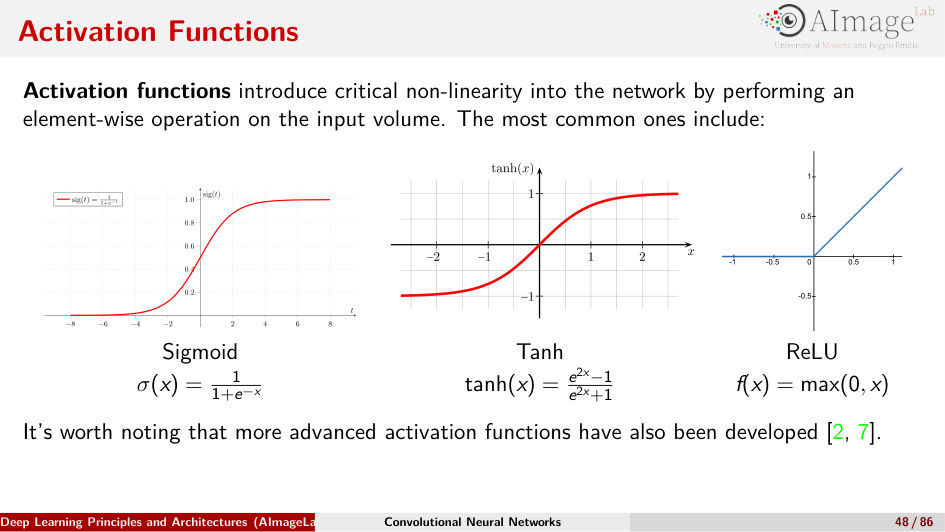
\includegraphics[keepaspectratio]{figure/fig_805f927f4b8485ec.png}} \pandocbounded{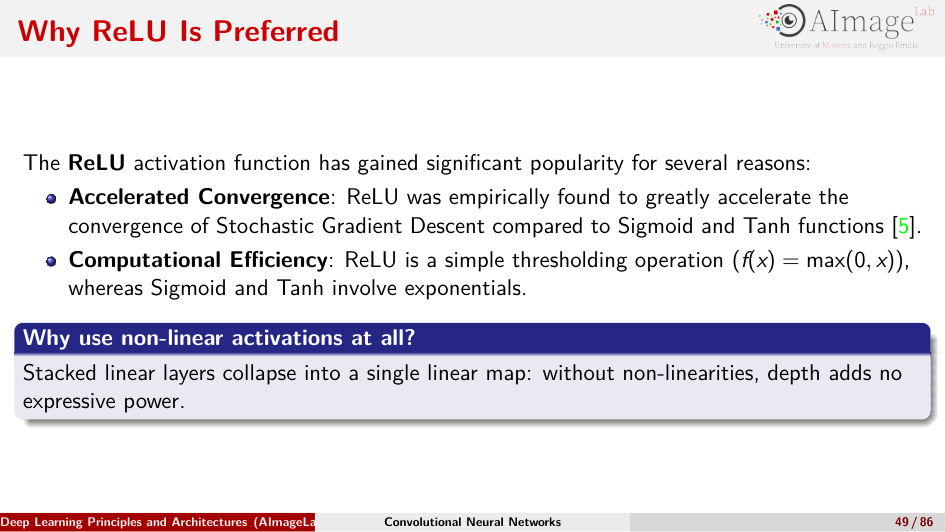
\includegraphics[keepaspectratio]{figure/fig_6c08c2ce08dc0745.png}}
% END F02-B0239

% BEGIN F02-B0240
\subsection{Dai Limiti di Sigmoide e Tanh al Successo della ReLU (slide 52--53)}\label{f02-r734}
% END F02-B0240

% BEGIN F02-B0241
Storicamente, le prime reti neurali impiegavano come attivazioni la \textbf{Sigmoide} o la \textbf{Tangente Iperbolica (Tanh)} (Slide 52):
% END F02-B0241

% BEGIN F02-B0242
\begin{center}
\begin{adjustbox}{max width=\linewidth}
$\displaystyle 
\sigma(x) = \frac{1}{1 + e^{-x}}, \qquad \tanh(x) = \frac{e^x - e^{-x}}{e^x + e^{-x}} = \frac{e^{2x} - 1}{e^{2x} + 1}
$
\end{adjustbox}
\end{center}
% END F02-B0242

% BEGIN F02-B0243
Entrambe queste funzioni presentano due gravi svantaggi nell\textquotesingle addestramento di reti profonde: 1. \textbf{Saturazione e scomparsa del gradiente (\emph{Vanishing Gradient})}: per valori di ingresso elevati (positivi o negativi), la curva si appiattisce asintoticamente. La derivata prima tende esponenzialmente a zero (\(\sigma'(x) \approx 0\)). Durante la retropropagazione, moltiplicando gradienti vicini allo zero lungo molti strati, il segnale di errore si annulla prima di raggiungere gli strati iniziali, bloccando l\textquotesingle apprendimento dei filtri. 2. \textbf{Costo computazionale elevato}: il calcolo degli esponenziali (\(e^{-x}\)) è operativamente dispendioso rispetto a operazioni aritmetiche elementari.
% END F02-B0243

% BEGIN F02-B0244
La \textbf{ReLU (Rectified Linear Unit)}, introdotta sistematicamente su larga scala proprio con AlexNet (Slide 53), definisce una semplice sogliatura a zero:
% END F02-B0244

% BEGIN F02-B0245
\begin{center}
\begin{adjustbox}{max width=\linewidth}
$\displaystyle 
\boxed{f(x) = \max(0, x)}
$
\end{adjustbox}
\end{center}
% END F02-B0245

% BEGIN F02-B0246
La ReLU garantisce vantaggi decisivi: * \textbf{Accelerazione drammatica della convergenza}: per tutti i valori positivi (\(x > 0\)), la derivata è costante e pari a 1 (\(\frac{df}{dx} = 1\)). Il gradiente non è attenuato dal solo fattore derivativo della ReLU sul semiasse positivo; rimangono gli effetti dei pesi e degli altri strati, consentendo alla discesa stocastica del gradiente (SGD) di convergere molto più rapidamente. * \textbf{Efficienza di calcolo estrema}: richiede una banale operazione di confronto logico a livello di registri hardware, senza esponenziali né divisioni.
% END F02-B0246

% BEGIN F02-B0247
\subsection{La Patologia del Dying ReLU e le Attivazioni Avanzate: Leaky ReLU ed ELU (slide 54)}\label{f02-r756}
% END F02-B0247

% BEGIN F02-B0248
Nonostante i suoi benefici, la ReLU standard manifesta una debolezza intrinseca, evidenziata dall\textquotesingle annotazione presente sulla Slide 54:
% END F02-B0248

% BEGIN F02-B0249
\begin{quote}
\emph{"Nella ReLU normale qualsiasi valore negativo viene tagliato a 0 e questo ferma l\textquotesingle apprendimento del modello."}
\end{quote}
% END F02-B0249

% BEGIN F02-B0250
\begin{itemize}
\tightlist
\item
  Un\textquotesingle attivazione negativa annulla il gradiente \textbf{attraverso quella posizione}, non l\textquotesingle apprendimento dell\textquotesingle intero modello. Un filtro condiviso può ricevere contributi da altre posizioni o esempi dove è attivo. Il problema del \emph{dying ReLU} riguarda unità che rimangono inattive su tutti o quasi tutti gli input rilevanti; non segue da un solo valore negativo e non è necessariamente irreversibile.
\end{itemize}
% END F02-B0250

% BEGIN F02-B0251
\begin{figure}[H]
\centering
\pandocbounded{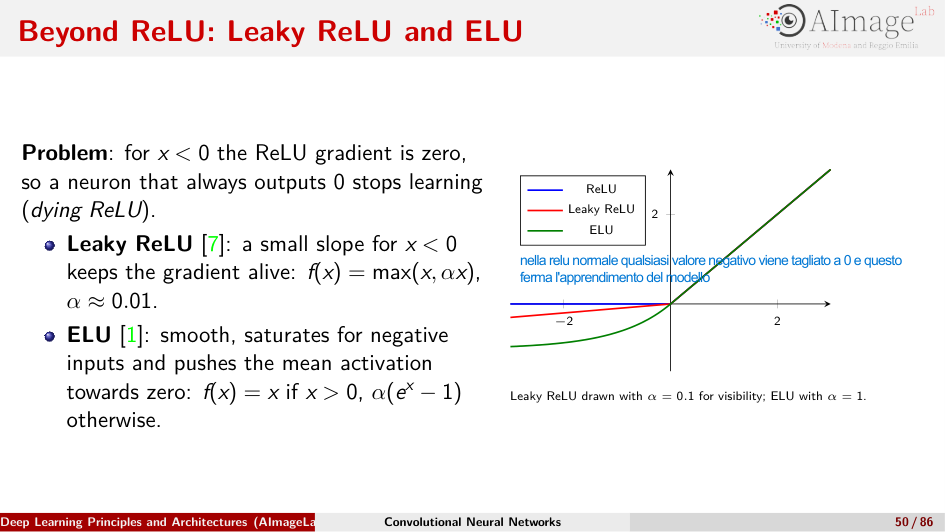
\includegraphics[keepaspectratio]{figure/fig_1afffea582f4d35e.png}}
\caption{Slide 54 -- Beyond ReLU: Leaky ReLU and ELU}
\end{figure}
% END F02-B0251

% BEGIN F02-B0252
Per sanare questa criticità sono state sviluppate due estensioni fondamentali (Slide 54):
% END F02-B0252

% BEGIN F02-B0253
\subsubsection{Leaky ReLU}\label{f02-r768}
% END F02-B0253

% BEGIN F02-B0254
La \textbf{Leaky ReLU} introduce una piccola pendenza lineare per la regione dei valori negativi, impedendo al gradiente di azzerarsi:
% END F02-B0254

% BEGIN F02-B0255
\begin{center}
\begin{adjustbox}{max width=\linewidth}
$\displaystyle 
\boxed{f(x) = \max(x, \alpha x) = \begin{cases} x & \text{se } x \ge 0 \\ \alpha x & \text{se } x < 0 \end{cases}}
$
\end{adjustbox}
\end{center}
% END F02-B0255

% BEGIN F02-B0256
dove \(\alpha\) è un iperparametro positivo molto piccolo (tipicamente fissato a \(\alpha = 0.01\); nella figura della Slide 54 è tracciato con \(\alpha = 0.1\) a scopo di visibilità grafica).
% END F02-B0256

% BEGIN F02-B0257
La derivata della Leaky ReLU vale:
% END F02-B0257

% BEGIN F02-B0258
\begin{center}
\begin{adjustbox}{max width=\linewidth}
$\displaystyle 
f'(x) = \begin{cases} 1 & \text{se } x > 0 \\ \alpha & \text{se } x < 0 \end{cases}
$
\end{adjustbox}
\end{center}
% END F02-B0258

% BEGIN F02-B0259
Poiché per \(x < 0\) la derivata vale \(\alpha \ne 0\), \textbf{il gradiente rimane vivo anche per attivazioni negative}, consentendo ai pesi del filtro di continuare a ricevere correzioni e di riattivarsi nelle iterazioni successive.
% END F02-B0259

% BEGIN F02-B0260
\subsubsection{ELU (Exponential Linear Unit)}\label{f02-r786}
% END F02-B0260

% BEGIN F02-B0261
L\textquotesingle{}\textbf{ELU (Exponential Linear Unit)} sostituisce la retta spezzata con un andamento esponenziale asintotico liscio nella semiretta negativa:
% END F02-B0261

% BEGIN F02-B0262
\begin{center}
\begin{adjustbox}{max width=\linewidth}
$\displaystyle 
\boxed{f(x) = \begin{cases} x & \text{se } x > 0 \\ \alpha (e^x - 1) & \text{se } x \le 0 \end{cases}}
$
\end{adjustbox}
\end{center}
% END F02-B0262

% BEGIN F02-B0263
(tipicamente impostata con \(\alpha = 1\)).
% END F02-B0263

% BEGIN F02-B0264
L\textquotesingle ELU è continua per ogni \(\alpha>0\). Le derivate laterali in zero sono \(\alpha\) e 1, quindi è differenziabile in zero \textbf{soltanto se \(\alpha=1\)}. Per \(x<0\) la derivata è \(\alpha e^x\): è positiva ma tende a zero per ingressi molto negativi. L\textquotesingle uscita tende a \(-\alpha\) e i valori negativi possono avvicinare la media delle attivazioni a zero, senza garantirne l\textquotesingle annullamento.
% END F02-B0264

% BEGIN F02-B0265
Con \(x=-2\), ReLU dà \(0\) e derivata \(0\); Leaky ReLU con \(\alpha=0.01\) dà \(-0.02\) e derivata \(0.01\); ELU con \(\alpha=1\) dà \(e^{-2}-1\approx-0.8647\) e derivata \(e^{-2}\approx0.1353\). Questi sono calcoli scalari applicati indipendentemente a ciascuna componente del tensore, senza cambiarne le dimensioni.
% END F02-B0265

% BEGIN F02-B0266
\begin{center}\rule{0.5\linewidth}{0.5pt}\end{center}
% END F02-B0266

% BEGIN F02-B0267
\section{Livelli di pooling: aggregazione locale e riduzione spaziale (slide 55--58)}\label{f02-r802}
% END F02-B0267

% BEGIN F02-B0268
Una convoluzione produce mappe di attivazione che descrivono pattern in posizioni diverse. Conservare tutte le posizioni a ogni profondità ha un costo di memoria e mantiene dettagli talvolta superflui per classificare. Il \textbf{pooling} riassume una finestra in un solo valore, riducendo la risoluzione quando lo stride è maggiore di uno.
% END F02-B0268

% BEGIN F02-B0269
L\textquotesingle operazione si applica \textbf{separatamente a ogni canale}: se entrano 16 mappe, ne escono 16. Il «kernel» indica qui la finestra di aggregazione, non pesi apprendibili. Dimensione della finestra, stride e funzione di aggregazione sono iperparametri; max e average pooling ordinari hanno \textbf{zero parametri apprendibili}, come annotato nella slide 55.
% END F02-B0269

% BEGIN F02-B0270
\begin{figure}[H]
\centering
\pandocbounded{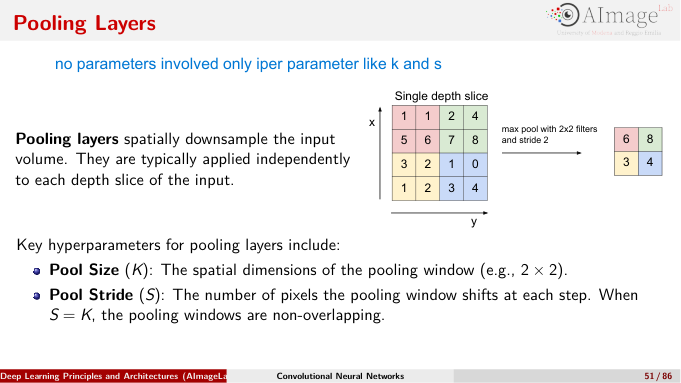
\includegraphics[keepaspectratio]{figure/fig_939ba149b22549ce.png}}
\caption{Slide 55 -- Finestra di max pooling e annotazione sui parametri}
\end{figure}
% END F02-B0270

% BEGIN F02-B0271
\subsection{Formule e dimensioni (slide 55--56)}\label{f02-r810}
% END F02-B0271

% BEGIN F02-B0272
Si usa \(X\in\mathbb{R}^{N\times C\times H\times W}\): batch \(N\), canali \(C\), altezza \(H\) e larghezza \(W\). Con finestra quadrata \(K\times K\), stride \(S\), nessun padding né dilatazione e indici spaziali da zero:
% END F02-B0272

% BEGIN F02-B0273
\begin{center}
\begin{adjustbox}{max width=\linewidth}
$\displaystyle 
\boxed{\begin{aligned}
Y^{\max}_{n,c,i,j}&=\max_{0\leq u,v<K}X_{n,c,iS+u,jS+v},\\
Y^{\mathrm{avg}}_{n,c,i,j}&=\frac1{K^2}\sum_{u=0}^{K-1}\sum_{v=0}^{K-1}X_{n,c,iS+u,jS+v}.
\end{aligned}}
$
\end{adjustbox}
\end{center}
% END F02-B0273

% BEGIN F02-B0274
Ogni uscita è uno scalare: il massimo seleziona il valore più alto fra i \(K^2\) elementi, la media ne somma i contributi e divide per il loro numero. Il massimo privilegia una risposta forte anche isolata; la media misura l\textquotesingle attivazione complessiva della regione. Un\textquotesingle attivazione non è necessariamente una probabilità: un valore 100 può essere semplicemente uno score.
% END F02-B0274

% BEGIN F02-B0275
La finestra di indice \(i\) parte dalla riga \(iS\) e deve soddisfare \(iS+K\leq H\). Quindi
% END F02-B0275

% BEGIN F02-B0276
\begin{center}
\begin{adjustbox}{max width=\linewidth}
$\displaystyle 
\begin{aligned}
i&\leq(H-K)/S,\\
i_{\max}&=\lfloor(H-K)/S\rfloor,\\
\boxed{H'}&=\boxed{\lfloor(H-K)/S\rfloor+1},\qquad
\boxed{W'}=\boxed{\lfloor(W-K)/S\rfloor+1}.
\end{aligned}
$
\end{adjustbox}
\end{center}
% END F02-B0276

% BEGIN F02-B0277
L\textquotesingle uscita è \(Y\in\mathbb{R}^{N\times C\times H'\times W'}\). Con \(K=S=2\) e dimensioni pari, entrambi gli assi si dimezzano e le attivazioni diventano un quarto. Batch e canali restano invariati. Con \(S=1\), invece, una griglia \(4\times4\) diventa \(3\times3\). Le finestre sono non sovrapposte per \(S=K\).
% END F02-B0277

% BEGIN F02-B0278
\begin{quote}
\textbf{Stride e riduzione}
\end{quote}
% END F02-B0278

% BEGIN F02-B0279
\begin{quote}
Il riferimento orale isolato a una configurazione usuale \(K=2,S=1\) contrasta con l\textquotesingle esempio e con la slide 57. La configurazione che dimezza entrambi gli assi è \(K=2,S=2\).
\end{quote}
% END F02-B0279

% BEGIN F02-B0280
\subsection{Esempio completo della slide 55 (slide 55--56)}\label{f02-r839}
% END F02-B0280

% BEGIN F02-B0281
Per un esempio e un canale:
% END F02-B0281

% BEGIN F02-B0282
\begin{center}
\begin{adjustbox}{max width=\linewidth}
$\displaystyle 
X=\begin{bmatrix}1&1&2&4\\5&6&7&8\\3&2&1&0\\1&2&3&4\end{bmatrix}\in\mathbb{R}^{4\times4}.
$
\end{adjustbox}
\end{center}
% END F02-B0282

% BEGIN F02-B0283
Con \(K=S=2\) si ottengono quattro finestre:
% END F02-B0283

% BEGIN F02-B0284
\begin{longtable}[]{@{}llrr@{}}
\toprule\noalign{}
Uscita & Valori & Massimo & Media \\
\midrule\noalign{}
\endhead
\bottomrule\noalign{}
\endlastfoot
\((0,0)\) & \(1,1,5,6\) & 6 & \(13/4=3.25\) \\
\((0,1)\) & \(2,4,7,8\) & 8 & \(21/4=5.25\) \\
\((1,0)\) & \(3,2,1,2\) & 3 & \(8/4=2\) \\
\((1,1)\) & \(1,0,3,4\) & 4 & \(8/4=2\) \\
\end{longtable}
% END F02-B0284

% BEGIN F02-B0285
\begin{center}
\begin{adjustbox}{max width=\linewidth}
$\displaystyle 
\boxed{Y^{\max}=\begin{bmatrix}6&8\\3&4\end{bmatrix}},\qquad
\boxed{Y^{\mathrm{avg}}=\begin{bmatrix}3.25&5.25\\2&2\end{bmatrix}}.
$
\end{adjustbox}
\end{center}
% END F02-B0285

% BEGIN F02-B0286
Le forme tornano: \(H'=W'=\lfloor(4-2)/2\rfloor+1=2\). La riduzione degli scalari è \((16-4)/16=75\%\). Un input \(N\times16\times8\times8\) diventa \(N\times16\times4\times4\): la medesima operazione viene ripetuta sui canali senza apprendere 16 nuovi filtri.
% END F02-B0286

% BEGIN F02-B0287
Zero parametri non significa assenza di backpropagation. Con massimo unico, la derivata rispetto agli elementi della finestra vale 1 nella posizione selezionata e 0 nelle altre; per la media vale \(1/K^2\) in ogni posizione. Sono le derivate delle due funzioni scalari. Se il gradiente in arrivo sulla prima uscita è 2, il massimo lo invia al valore 6; la media invia \(2/4=0.5\) a ciascun valore. Con massimi uguali occorre una convenzione per il sottogradiente; con finestre sovrapposte i contributi alla stessa posizione si sommano.
% END F02-B0287

% BEGIN F02-B0288
\subsection{Robustezza locale, gerarchia e campo recettivo (slide 57)}\label{f02-r865}
% END F02-B0288

% BEGIN F02-B0289
Il massimo di \((100,2,4,3)\) rimane 100 qualunque sia la posizione del 100 \textbf{entro la finestra}. Se il canale rileva un cerchio, interessa sapere che una forte risposta esiste nella regione, anche perdendone la coordinata precisa. La media è invece \(109/4=27.25\): una risposta isolata viene attenuata dai valori piccoli circostanti. Questa è la motivazione intuitiva per usare spesso il massimo negli stadi locali e la media per una descrizione complessiva; non dimostra che il max pooling sia sempre superiore.
% END F02-B0289

% BEGIN F02-B0290
La robustezza è limitata: se il 100 attraversa il confine fra due finestre cambia l\textquotesingle uscita. Pooling e stride non garantiscono invarianza a qualunque traslazione dell\textquotesingle immagine.
% END F02-B0290

% BEGIN F02-B0291
L\textquotesingle annotazione «gerarchia di concetti» si riferisce alla composizione progressiva delle rappresentazioni: i primi filtri descrivono bordi e contrasti, i successivi combinano risposte su regioni più estese. Eliminare dettagli di posizione può favorire l\textquotesingle astrazione, ma il pooling non produce da solo significati semantici: questi dipendono dai filtri appresi e dal compito.
% END F02-B0291

% BEGIN F02-B0292
\begin{figure}[H]
\centering
\pandocbounded{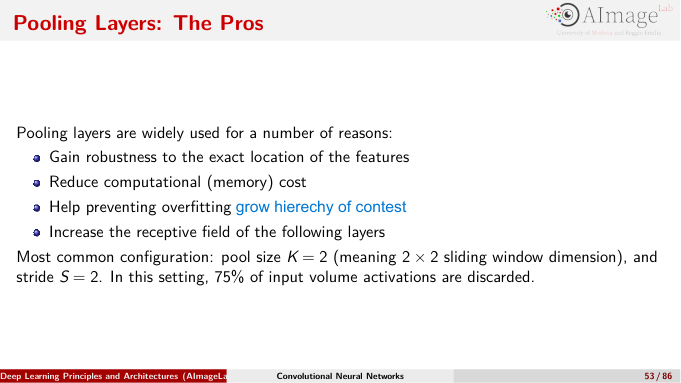
\includegraphics[keepaspectratio]{figure/fig_5e1ba8eca2281d23.png}}
\caption{Slide 57 -- Vantaggi del pooling e gerarchia}
\end{figure}
% END F02-B0292

% BEGIN F02-B0293
Con campo recettivo \(r\) e distanza \(j\) fra uscite adiacenti, misurata sull\textquotesingle immagine iniziale:
% END F02-B0293

% BEGIN F02-B0294
\begin{center}
\begin{adjustbox}{max width=\linewidth}
$\displaystyle \boxed{r_{\mathrm{out}}=r_{\mathrm{in}}+(K-1)j_{\mathrm{in}},\qquad j_{\mathrm{out}}=S j_{\mathrm{in}}.}$
\end{adjustbox}
\end{center}
% END F02-B0294

% BEGIN F02-B0295
La prima formula unisce \(K\) campi i cui centri distano \(j_{\mathrm{in}}\); la seconda esprime il salto di \(S\) posizioni. Dopo una convoluzione \(3\times3\) a stride 1 si ha \(r=3,j=1\). Un pooling \(2\times2\) a stride 2 dà \(r=4,j=2\); un\textquotesingle altra convoluzione \(3\times3\) dà \(r=4+2\cdot2=8\). L\textquotesingle uscita può dipendere da una regione \(8\times8\) dell\textquotesingle input originale. Si tratta del campo recettivo potenziale, distinto dalle posizioni effettivamente selezionate dal massimo.
% END F02-B0295

% BEGIN F02-B0296
Il pooling riduce la memoria delle attivazioni e il lavoro successivo. La perdita di dettagli può limitare dipendenze da peculiarità del training set, ma non garantisce l\textquotesingle assenza di overfitting.
% END F02-B0296

% BEGIN F02-B0297
\subsection{Il limite: perdita di localizzazione (slide 58)}\label{f02-r883}
% END F02-B0297

% BEGIN F02-B0298
Nella classificazione può bastare sapere che un oggetto è presente; nella segmentazione semantica occorre assegnare una classe a ogni pixel. Una riduzione aggressiva della risoluzione può cancellare confini e oggetti piccoli.
% END F02-B0298

% BEGIN F02-B0299
\begin{figure}[H]
\centering
\pandocbounded{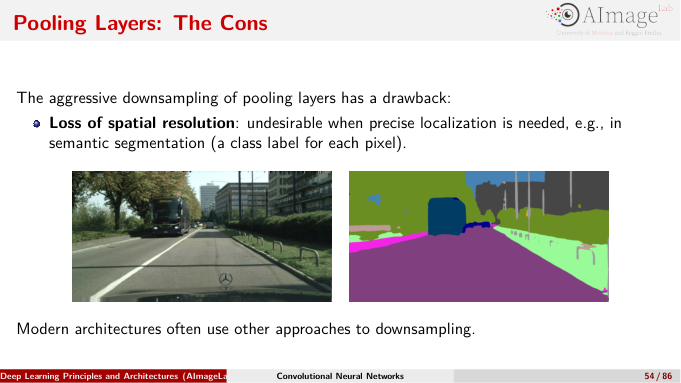
\includegraphics[keepaspectratio]{figure/fig_b31108d56dc62dd7.png}}
\caption{Slide 58 -- Risoluzione e segmentazione}
\end{figure}
% END F02-B0299

% BEGIN F02-B0300
Il pooling va scelto in funzione del compito. Questo non implica che ogni modello di segmentazione debba escluderlo, ma che la gestione della risoluzione richieda attenzione. Le alternative architetturali non vengono sviluppate qui.
% END F02-B0300

% BEGIN F02-B0301
\section{Dalle feature al classificatore: pooling adattivo (slide 59)}\label{f02-r891}
% END F02-B0301

% BEGIN F02-B0302
L\textquotesingle estrattore produce \(X\in\mathbb{R}^{N\times C\times h\times w}\). Un livello denso richiede un numero fisso di ingressi, perché la sua matrice dei pesi ha un numero fisso di colonne. Occorre quindi rendere compatibile una griglia dipendente dalla risoluzione con un classificatore di forma fissata.
% END F02-B0302

% BEGIN F02-B0303
\subsection{Flattening e risoluzione dell\textquotesingle ingresso (slide 59)}\label{f02-r895}
% END F02-B0303

% BEGIN F02-B0304
Il flattening riordina gli elementi senza aggregarli:
% END F02-B0304

% BEGIN F02-B0305
\begin{center}
\begin{adjustbox}{max width=\linewidth}
$\displaystyle \boxed{N\times C\times h\times w\ \longrightarrow\ N\times D,\qquad D=Chw.}$
\end{adjustbox}
\end{center}
% END F02-B0305

% BEGIN F02-B0306
Da \(16\times8\times8\) si ottengono 1024 elementi. Se un\textquotesingle immagine più grande produce \(16\times12\times12\), diventano 2304: una matrice \(W\in\mathbb{R}^{q\times1024}\) non può moltiplicare un vettore di lunghezza 2304. La flessibilità spaziale della convoluzione non rende automaticamente flessibile la testa densa.
% END F02-B0306

% BEGIN F02-B0307
Se la risoluzione è fissa, il flattening diretto è valido e conserva tutte le attivazioni. Non è necessariamente migliore: richiede più pesi e impone quella forma. Ridimensionare preventivamente le immagini è possibile, ma introduce interpolazione e, se si altera il rapporto degli assi, deformazione geometrica.
% END F02-B0307

% BEGIN F02-B0308
\subsection{Global average pooling e posizione esatta nella rete (slide 59)}\label{f02-r905}
% END F02-B0308

% BEGIN F02-B0309
La media globale sostituisce ciascun canale con un solo scalare:
% END F02-B0309

% BEGIN F02-B0310
\begin{center}
\begin{adjustbox}{max width=\linewidth}
$\displaystyle \boxed{z_{n,c}=\frac1{hw}\sum_{i=0}^{h-1}\sum_{j=0}^{w-1}X_{n,c,i,j}.}$
\end{adjustbox}
\end{center}
% END F02-B0310

% BEGIN F02-B0311
È l\textquotesingle average pooling con una finestra estesa a tutta la mappa: si sommano \(hw\) elementi e si divide per il loro numero. Il volume diventa \(N\times C\times1\times1\) e un successivo flattening produce \(N\times C\), indipendentemente da \(h,w\).
% END F02-B0311

% BEGIN F02-B0312
Per due canali
% END F02-B0312

% BEGIN F02-B0313
\begin{center}
\begin{adjustbox}{max width=\linewidth}
$\displaystyle X_1=\begin{bmatrix}1&3\\5&7\end{bmatrix},\qquad X_2=\begin{bmatrix}2&2\\6&10\end{bmatrix},$
\end{adjustbox}
\end{center}
% END F02-B0313

% BEGIN F02-B0314
si ottiene \(z=[16/4,20/4]^T=[4,5]^T\in\mathbb{R}^2\). Un classificatore con \(q\) uscite impiega \(W\in\mathbb{R}^{q\times C}\), \(b\in\mathbb{R}^q\):
% END F02-B0314

% BEGIN F02-B0315
\begin{center}
\begin{adjustbox}{max width=\linewidth}
$\displaystyle \boxed{s=Wz+b\in\mathbb{R}^q,\qquad P=qC+q=q(C+1).}$
\end{adjustbox}
\end{center}
% END F02-B0315

% BEGIN F02-B0316
Con \(q=3\), \(W=\begin{bmatrix}1&0\\0&1\\1&-1\end{bmatrix}\) e \(b=0\), gli score sono \([4,5,-1]^T\). I sei pesi e tre bias danno nove parametri: sono del classificatore, non del pooling. Una softmax finale può convertirli in probabilità del modello.
% END F02-B0316

% BEGIN F02-B0317
Il dubbio «solo nell\textquotesingle ultimo layer: dove?» si risolve localizzando l\textquotesingle interfaccia: \textbf{dopo le ultime mappe dell\textquotesingle estrattore convoluzionale, prima del flattening e dell\textquotesingle MLP}, non dopo gli score finali.
% END F02-B0317

% BEGIN F02-B0318
\pandocbounded{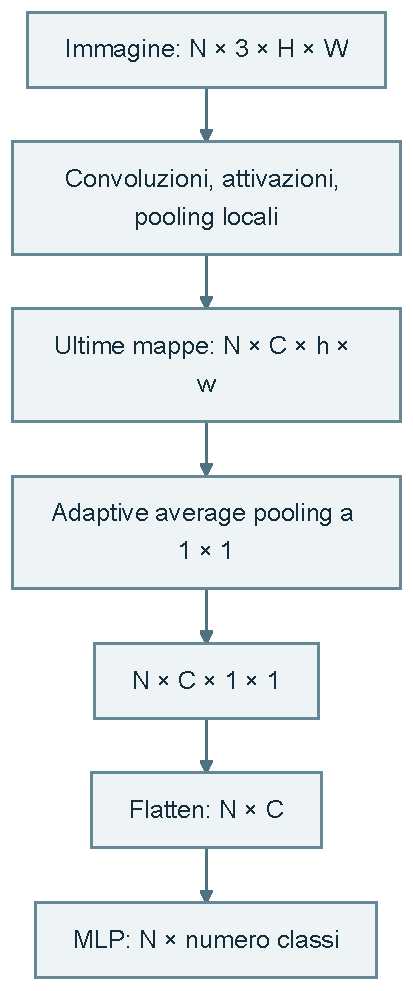
\includegraphics[keepaspectratio]{figure/diagramma_f02_06.pdf}}
% END F02-B0318

% BEGIN F02-B0319
\begin{figure}[H]
\centering
\pandocbounded{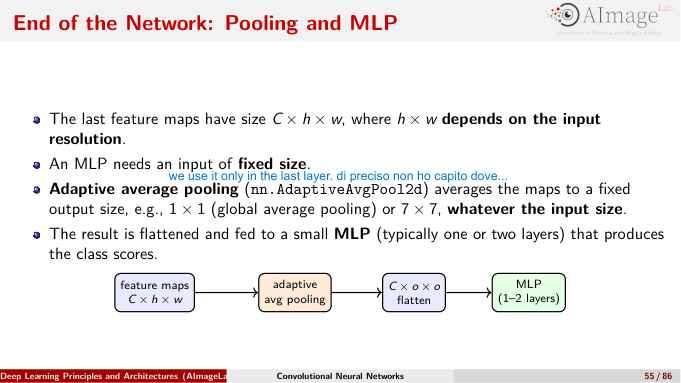
\includegraphics[keepaspectratio]{figure/fig_2feaa48e46e8677b.png}}
\caption{Slide 59 -- Collegamento fra estrattore e MLP}
\end{figure}
% END F02-B0319

% BEGIN F02-B0320
Il pooling \textbf{adattivo} fissa la dimensione di uscita adattando le regioni di aggregazione all\textquotesingle ingresso. L\textquotesingle uscita \(1\times1\) coincide con la media globale; una griglia fissa \(o\times o\), come \(7\times7\) nella slide, produce \(Co^2\) ingressi per l\textquotesingle MLP. Non si elimina il flattening: lo si applica dopo aver fissato la forma. Questa collocazione è il disegno discusso, non un divieto matematico di usare pooling adattivo altrove.
% END F02-B0320

% BEGIN F02-B0321
Con \(C=16,q=10\), il flattening diretto di \(8\times8\) richiede \(10(1024+1)=10250\) parametri; la media globale richiede \(10(16+1)=170\). Si risparmiano pesi perdendo disposizione spaziale. Più canali possono arricchire la descrizione, ma non ricostruiscono automaticamente le posizioni eliminate.
% END F02-B0321

% BEGIN F02-B0322
\section{LeNet e AlexNet: evoluzione delle CNN (slide 60--62)}\label{f02-r941}
% END F02-B0322

% BEGIN F02-B0323
Le architetture condividono convoluzioni, attivazioni, riduzione spaziale e classificazione, ma differiscono per profondità, kernel e canali. Queste scelte determinano campo recettivo e costo.
% END F02-B0323

% BEGIN F02-B0324
\subsection{LeNet: riconoscimento di cifre (slide 61)}\label{f02-r945}
% END F02-B0324

% BEGIN F02-B0325
LeNet mostra una pipeline completa per caratteri manoscritti: un\textquotesingle immagine a un canale \(32\times32\) attraversa filtri \(5\times5\) e sottocampionamenti. Il modello storico usa non linearità sigmoidi e sottocampionamento basato su medie; non va reinterpretato come una rete con ReLU e max pooling in ogni blocco.
% END F02-B0325

% BEGIN F02-B0326
\begin{figure}[H]
\centering
\pandocbounded{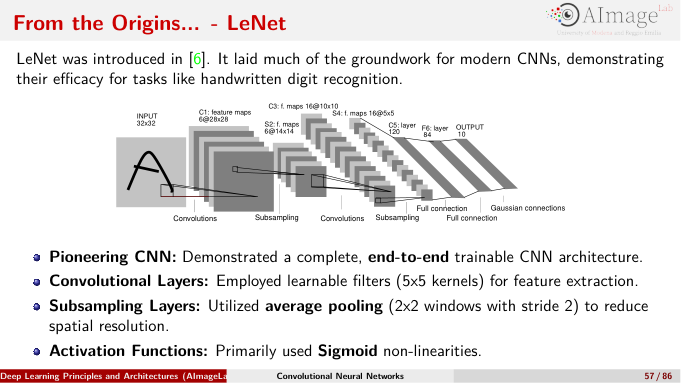
\includegraphics[keepaspectratio]{figure/fig_90e9546e7e5d9991.png}}
\caption{Slide 61 -- LeNet}
\end{figure}
% END F02-B0326

% BEGIN F02-B0327
\pandocbounded{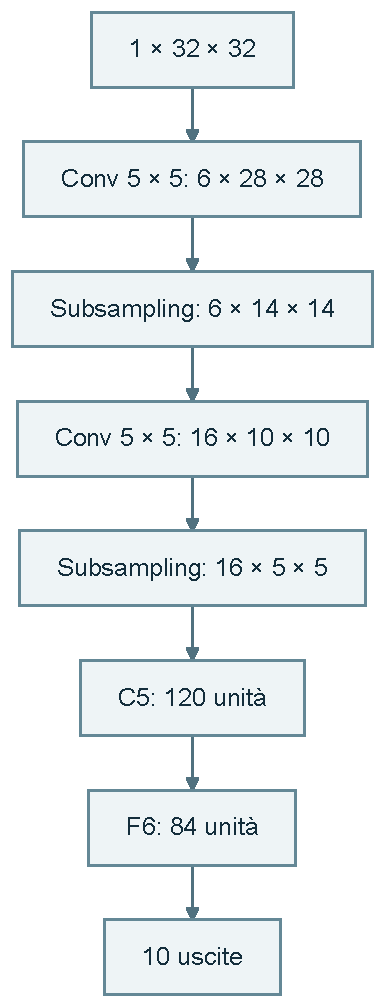
\includegraphics[keepaspectratio]{figure/diagramma_f02_07.pdf}}
% END F02-B0327

% BEGIN F02-B0328
Senza padding, \(32-5+1=28\); il sottocampionamento dimezza a 14. La convoluzione successiva dà \(14-5+1=10\) e il pooling porta a 5. Una finestra \(5\times5\) sull\textquotesingle ultima mappa copre tutta la sua estensione e dà un valore per filtro. La figura riporta connessioni gaussiane all\textquotesingle uscita, non una moderna softmax. Il conteggio zero dei parametri del pooling puro non va esteso automaticamente a ogni variante storica di sottocampionamento.
% END F02-B0328

% BEGIN F02-B0329
\subsection{AlexNet: scala computazionale e ReLU (slide 62)}\label{f02-r964}
% END F02-B0329

% BEGIN F02-B0330
AlexNet è associata al risultato ImageNet del 2012. Contiene \textbf{otto livelli con parametri}, cinque convoluzionali e tre fully connected; il conteggio non include separatamente ReLU e pooling. Utilizza un kernel iniziale \(11\times11\), ReLU e addestramento su due GPU nella realizzazione illustrata.
% END F02-B0330

% BEGIN F02-B0331
\begin{figure}[H]
\centering
\pandocbounded{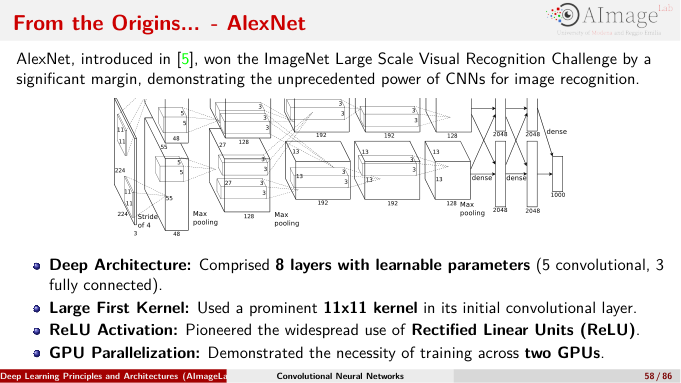
\includegraphics[keepaspectratio]{figure/fig_8ebd502982112089.png}}
\caption{Slide 62 -- AlexNet}
\end{figure}
% END F02-B0331

% BEGIN F02-B0332
Un kernel ampio aumenta rapidamente il campo recettivo quando ci sono pochi stadi convoluzionali, pagando più pesi. A canali fissati, passare da \(3\times3\) a \(11\times11\) moltiplica i pesi per \(121/9\approx13.44\). Il kernel grande non riduce da solo la risoluzione di un fattore fissato: contano anche stride e padding.
% END F02-B0332

% BEGIN F02-B0333
La GPU ha reso praticabile l\textquotesingle addestramento su larga scala; la ReLU evita la saturazione sul semiasse positivo. Non ne segue che AlexNet sia la prima rete profonda in assoluto o che due GPU siano necessarie per ogni CNN. Le indicazioni storiche esitanti nella trascrizione non vengono trasformate in fatti aggiuntivi.
% END F02-B0333

% BEGIN F02-B0334
\section{VGG: distribuire la capacità lungo la profondità (slide 63--68)}\label{f02-r974}
% END F02-B0334

% BEGIN F02-B0335
VGG, dal nome \textbf{Visual Geometry Group}, usa sequenze regolari di piccole convoluzioni \(3\times3\). L\textquotesingle elaborazione è distribuita lungo la profondità, costruendo gradualmente rappresentazioni più ampie. I pesi preaddestrati hanno inoltre favorito il trasferimento delle rappresentazioni fra compiti.
% END F02-B0335

% BEGIN F02-B0336
\subsection{Piccoli kernel e campo recettivo (slide 63--64)}\label{f02-r978}
% END F02-B0336

% BEGIN F02-B0337
A stride 1 e senza dilatazione, ogni convoluzione \(3\times3\) aggiunge due posizioni per asse:
% END F02-B0337

% BEGIN F02-B0338
\begin{center}
\begin{adjustbox}{max width=\linewidth}
$\displaystyle \boxed{r_L=1+\sum_{\ell=1}^L(3-1)=1+2L.}$
\end{adjustbox}
\end{center}
% END F02-B0338

% BEGIN F02-B0339
Due livelli hanno campo recettivo \(5\times5\), tre \(7\times7\). Non sono però equivalenti a un solo filtro grande: le attivazioni intermedie introducono ulteriori non linearità.
% END F02-B0339

% BEGIN F02-B0340
Supponendo \textbf{\(C\) canali in ingresso, in uscita e in tutti gli strati intermedi}, ogni coppia di canali possiede \(K^2\) pesi. Pertanto:
% END F02-B0340

% BEGIN F02-B0341
\begin{center}
\begin{adjustbox}{max width=\linewidth}
$\displaystyle 
\boxed{\begin{aligned}
P_{7\times7}&=49C^2,& P_{3\times(3\times3)}&=27C^2,\\
P_{5\times5}&=25C^2,& P_{2\times(3\times3)}&=18C^2.
\end{aligned}}
$
\end{adjustbox}
\end{center}
% END F02-B0341

% BEGIN F02-B0342
Nel primo confronto il risparmio è \(22/49\approx44.90\%\). Con \(C=64\), si passa da \(200704\) a \(110592\) pesi. Includendo i bias, sono \(200768\) contro \(110784\), perché tre strati hanno tre vettori di bias. La sequenza offre tre ReLU invece di una. Con canali intermedi diversi il conteggio va rifatto: il risparmio non vale per qualunque architettura.
% END F02-B0342

% BEGIN F02-B0343
\begin{figure}[H]
\centering
\pandocbounded{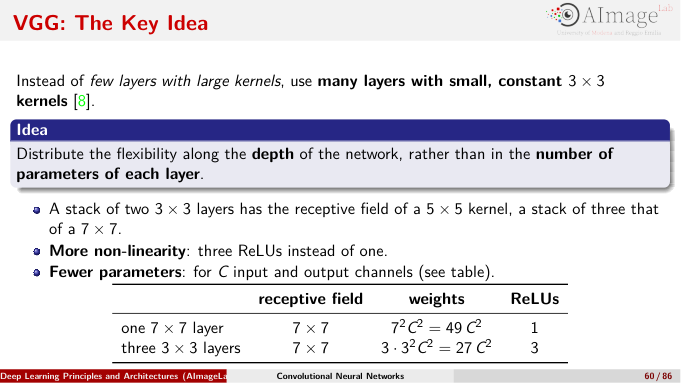
\includegraphics[keepaspectratio]{figure/fig_897b43cf81048614.png}}
\caption{Slide 64 -- Kernel grande e sequenza di kernel piccoli}
\end{figure}
% END F02-B0343

% BEGIN F02-B0344
Una costruzione graduale lascia spazio alla condivisione di feature fra classi: bordi e texture possono contribuire a categorie diverse prima di essere combinati in parti specifiche. È una motivazione progettuale, non una garanzia che aggiungere livelli migliori sempre l\textquotesingle accuratezza.
% END F02-B0344

% BEGIN F02-B0345
\subsection{VGG16: percorso delle dimensioni (slide 65--66)}\label{f02-r1001}
% END F02-B0345

% BEGIN F02-B0346
VGG16 contiene 13 convoluzioni e 3 livelli densi: \textbf{16 livelli con pesi}. Le convoluzioni \(3\times3\) hanno stride 1 e padding 1, mentre cinque max pooling \(2\times2\) a stride 2 dimezzano progressivamente gli assi dell\textquotesingle ingresso RGB \(224\times224\).
% END F02-B0346

% BEGIN F02-B0347
\begin{longtable}[]{@{}
  >{\raggedright\arraybackslash}p{(\linewidth - 6\tabcolsep) * \real{0.2500}}
  >{\raggedright\arraybackslash}p{(\linewidth - 6\tabcolsep) * \real{0.2500}}
  >{\raggedright\arraybackslash}p{(\linewidth - 6\tabcolsep) * \real{0.2500}}
  >{\raggedright\arraybackslash}p{(\linewidth - 6\tabcolsep) * \real{0.2500}}@{}}
\toprule\noalign{}
\begin{minipage}[b]{\linewidth}\raggedright
Blocco
\end{minipage} & \begin{minipage}[b]{\linewidth}\raggedright
Successione dei canali
\end{minipage} & \begin{minipage}[b]{\linewidth}\raggedright
Forma dopo le convoluzioni, senza batch
\end{minipage} & \begin{minipage}[b]{\linewidth}\raggedright
Forma dopo il pooling
\end{minipage} \\
\midrule\noalign{}
\endhead
\bottomrule\noalign{}
\endlastfoot
1 & \(3\to64\to64\) & \(64\times224\times224\) & \(64\times112\times112\) \\
2 & \(64\to128\to128\) & \(128\times112\times112\) & \(128\times56\times56\) \\
3 & \(128\to256\to256\to256\) & \(256\times56\times56\) & \(256\times28\times28\) \\
4 & \(256\to512\to512\to512\) & \(512\times28\times28\) & \(512\times14\times14\) \\
5 & \(512\to512\to512\to512\) & \(512\times14\times14\) & \(512\times7\times7\) \\
\end{longtable}
% END F02-B0347

% BEGIN F02-B0348
Le forme derivano da \((H-3+2)+1=H\) per le convoluzioni e \(H/2\) per i pooling su dimensioni pari. La catena spaziale è \(224\to112\to56\to28\to14\to7\). Il flattening produce \(512\cdot7\cdot7=25088\) ingressi per i livelli \(4096\to4096\to1000\).
% END F02-B0348

% BEGIN F02-B0349
\pandocbounded{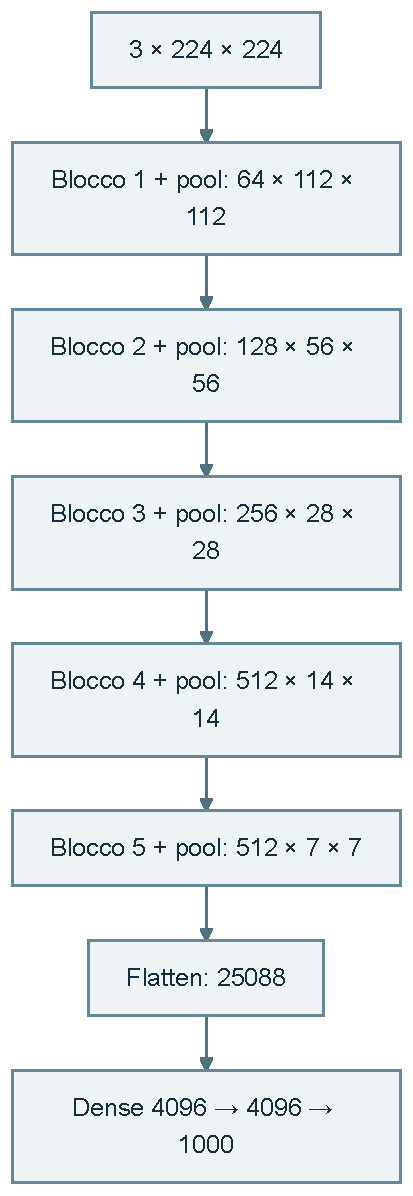
\includegraphics[keepaspectratio]{figure/diagramma_f02_08.pdf}}
% END F02-B0349

% BEGIN F02-B0350
\pandocbounded{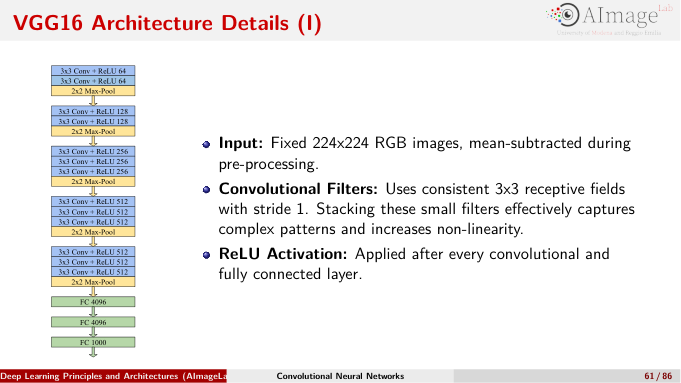
\includegraphics[keepaspectratio]{figure/fig_efe9830d74d66fbe.png}} \pandocbounded{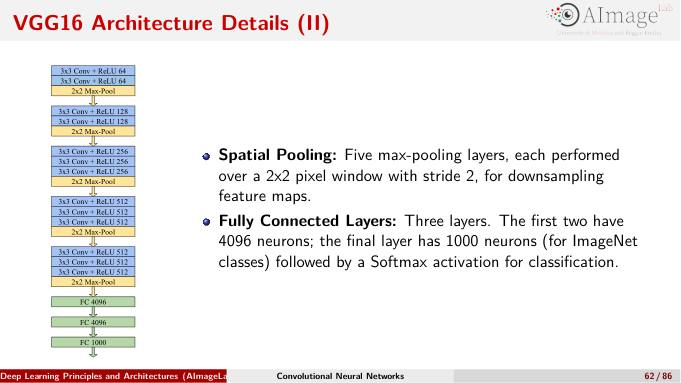
\includegraphics[keepaspectratio]{figure/fig_542d643edce8713b.png}}
% END F02-B0350

% BEGIN F02-B0351
La sottrazione della media all\textquotesingle ingresso è pre-processamento, distinto dalla Batch Normalization. Le ReLU seguono convoluzioni e livelli densi nascosti; gli score finali alimentano la softmax. L\textquotesingle espressione «dopo ogni fully connected» della slide 65 va letta insieme alla slide 66, che distingue l\textquotesingle uscita di classificazione.
% END F02-B0351

% BEGIN F02-B0352
\subsection{Dove sono i 138 milioni di parametri? (slide 67--68)}\label{f02-r1031}
% END F02-B0352

% BEGIN F02-B0353
Un livello denso ha un peso per ogni coppia ingresso--uscita e un bias per uscita:
% END F02-B0353

% BEGIN F02-B0354
\begin{center}
\begin{adjustbox}{max width=\linewidth}
$\displaystyle \boxed{P_{\mathrm{dense}}=d_{\mathrm{out}}d_{\mathrm{in}}+d_{\mathrm{out}}.}$
\end{adjustbox}
\end{center}
% END F02-B0354

% BEGIN F02-B0355
La domanda della slide 67 riguarda il \textbf{primo fully connected}, che riceve tutti i 25088 elementi:
% END F02-B0355

% BEGIN F02-B0356
\begin{center}
\begin{adjustbox}{max width=\linewidth}
$\displaystyle 
\begin{aligned}
P_{\mathrm{FC1}}&=25088\cdot4096+4096=102764544,\\
P_{\mathrm{FC2}}&=4096\cdot4096+4096=16781312,\\
P_{\mathrm{FC3}}&=4096\cdot1000+1000=4097000,\\
P_{\mathrm{FC}}&=123642856.
\end{aligned}
$
\end{adjustbox}
\end{center}
% END F02-B0356

% BEGIN F02-B0357
Per le convoluzioni si applica \(P=C_{\mathrm{out}}(9C_{\mathrm{in}}+1)\):
% END F02-B0357

% BEGIN F02-B0358
\begin{longtable}[]{@{}llr@{}}
\toprule\noalign{}
Blocco & Calcolo, bias inclusi & Totale \\
\midrule\noalign{}
\endhead
\bottomrule\noalign{}
\endlastfoot
1 & \(64(9\cdot3+1)+64(9\cdot64+1)\) & 38720 \\
2 & \(128(9\cdot64+1)+128(9\cdot128+1)\) & 221440 \\
3 & \(256(9\cdot128+1)+2\cdot256(9\cdot256+1)\) & 1475328 \\
4 & \(512(9\cdot256+1)+2\cdot512(9\cdot512+1)\) & 5899776 \\
5 & \(3\cdot512(9\cdot512+1)\) & 7079424 \\
Totale convoluzioni & somma dei cinque blocchi & \textbf{14714688} \\
\end{longtable}
% END F02-B0358

% BEGIN F02-B0359
Il totale è \(14714688+123642856=138357544\), circa 138 milioni. La parte densa contiene l\textquotesingle89.36\% dei parametri. Le cifre della slide 68 sono arrotondate in milioni e rappresentano soprattutto i pesi, perciò differiscono leggermente dai conti con bias. La percentuale dei pesi non coincide con quella del tempo di calcolo: una convoluzione riutilizza ciascun peso in molte posizioni.
% END F02-B0359

% BEGIN F02-B0360
\begin{figure}[H]
\centering
\pandocbounded{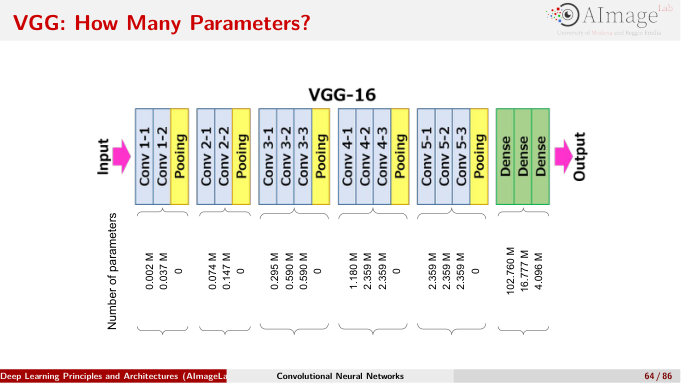
\includegraphics[keepaspectratio]{figure/fig_fa679b7b4b0dd4aa.png}}
\caption{Slide 68 -- Distribuzione dei parametri VGG16}
\end{figure}
% END F02-B0360

% BEGIN F02-B0361
\section{Profondità e residual learning: ResNet (slide 69--75)}\label{f02-r1063}
% END F02-B0361

% BEGIN F02-B0362
\subsection{Il problema della degradazione (slide 69--72)}\label{f02-r1065}
% END F02-B0362

% BEGIN F02-B0363
Aggiungere livelli a una rete tradizionale può peggiorare \textbf{sia training sia test}. Questo caso non è spiegato semplicemente dall\textquotesingle overfitting: una rete che memorizza meglio il training avrebbe tipicamente un errore di training inferiore; qui peggiora già l\textquotesingle ottimizzazione sui dati noti.
% END F02-B0363

% BEGIN F02-B0364
In linea di principio la rete più profonda potrebbe riprodurre quella corta facendo calcolare l\textquotesingle identità ai livelli aggiuntivi. La difficoltà è trovare quella configurazione durante l\textquotesingle addestramento: maggiore capacità non implica automaticamente maggiore facilità di ottimizzazione.
% END F02-B0364

% BEGIN F02-B0365
\pandocbounded{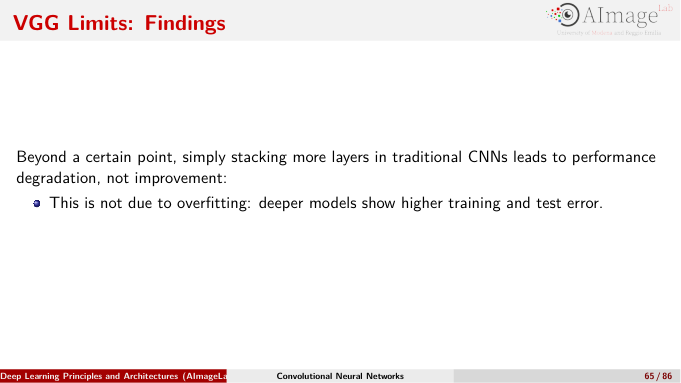
\includegraphics[keepaspectratio]{figure/fig_d8b838549cce650a.png}} \pandocbounded{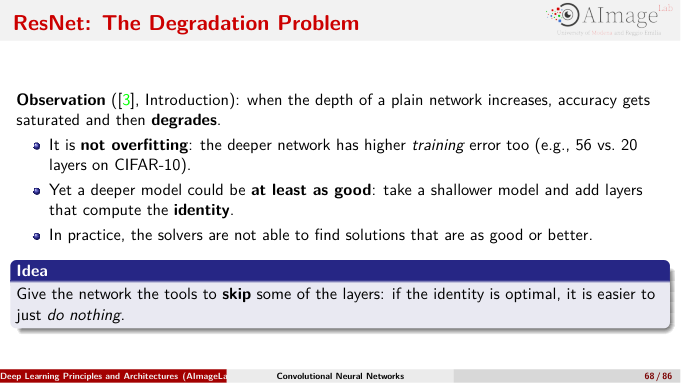
\includegraphics[keepaspectratio]{figure/fig_5d14ccdd6bd8b5d2.png}}
% END F02-B0365

% BEGIN F02-B0366
Per la catena scalare \(h_\ell=f_\ell(h_{\ell-1})\), applicando ripetutamente la regola della catena:
% END F02-B0366

% BEGIN F02-B0367
\begin{center}
\begin{adjustbox}{max width=\linewidth}
$\displaystyle \boxed{\frac{\partial\mathcal L}{\partial h_0}=\frac{\partial\mathcal L}{\partial h_L}\prod_{\ell=1}^{L}f'_\ell(h_{\ell-1}).}$
\end{adjustbox}
\end{center}
% END F02-B0367

% BEGIN F02-B0368
Ogni passo introduce un fattore: \(\partial\mathcal L/\partial h_{\ell-1}=(\partial\mathcal L/\partial h_\ell)f'_\ell\). Venti fattori 0.5 danno \(9.54\cdot10^{-7}\); venti fattori 2 danno 1048576. Sono esempi di gradiente che svanisce o esplode. Nel caso vettoriale compaiono prodotti di Jacobiane. L\textquotesingle instabilità è una difficoltà importante, ma non dimostra di esaurire ogni causa della degradazione.
% END F02-B0368

% BEGIN F02-B0369
\subsection{Blocco residuo e significato della shortcut (slide 71--74)}\label{f02-r1080}
% END F02-B0369

% BEGIN F02-B0370
Invece di apprendere direttamente \(H(x)\), si apprende la correzione rispetto all\textquotesingle ingresso:
% END F02-B0370

% BEGIN F02-B0371
\begin{center}
\begin{adjustbox}{max width=\linewidth}
$\displaystyle \boxed{F(x;\theta)=H(x)-x,\qquad H(x)=x+F(x;\theta).}$
\end{adjustbox}
\end{center}
% END F02-B0371

% BEGIN F02-B0372
La relazione si ricava isolando la differenza fra uscita e ingresso. Per \(x\in\mathbb{R}^{N\times C\times H\times W}\), il ramo \(F\) deve avere la stessa forma: la somma è elemento per elemento. Per rappresentare l\textquotesingle identità basta porre \(F(x)=0\).
% END F02-B0372

% BEGIN F02-B0373
\pandocbounded{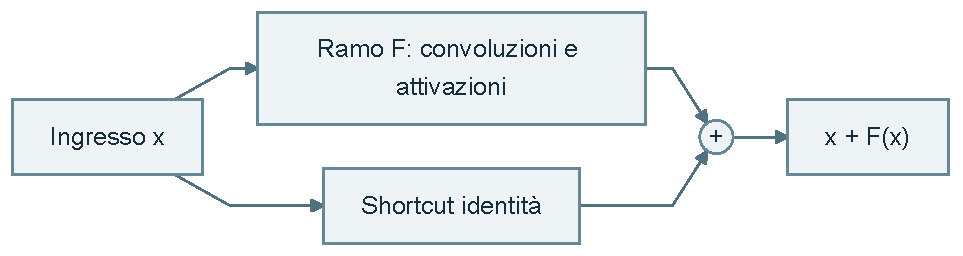
\includegraphics[keepaspectratio]{figure/diagramma_f02_09.pdf}}
% END F02-B0373

% BEGIN F02-B0374
\pandocbounded{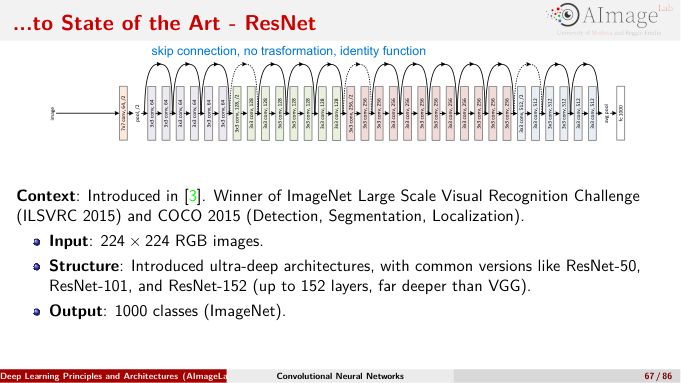
\includegraphics[keepaspectratio]{figure/fig_7b8f968adf2a5a58.png}} \pandocbounded{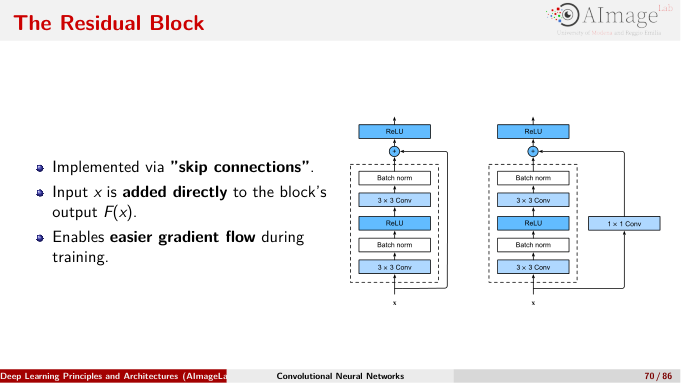
\includegraphics[keepaspectratio]{figure/fig_231b0a71661aabe3.png}}
% END F02-B0374

% BEGIN F02-B0375
\textbf{Entrambi i rami sono calcolati e poi sommati.} Non si evita fisicamente l\textquotesingle esecuzione di un ramo, non si confrontano i risultati per scegliere il migliore e non si scarta il ramo meno utile. «Ignorare il blocco» significa che il suo contributo appreso può essere vicino a zero, pur rimanendo il costo del calcolo.
% END F02-B0375

% BEGIN F02-B0376
Con \(x=[2,-1]^T\) e \(F(x)=0.25x\), il ramo produce \([0.5,-0.25]^T\) e la somma è \([2.5,-1.25]^T\). Se il coefficiente diventa zero, l\textquotesingle uscita è \(x\). La stessa funzione può produrre correzioni diverse per input diversi senza un selettore esterno di percorsi.
% END F02-B0376

% BEGIN F02-B0377
L\textquotesingle annotazione «nessuna trasformazione, identità» vale quando le forme coincidono. La figura 74 mostra anche una convoluzione \(1\times1\) sulla shortcut, necessaria quando cambiano canali o risoluzione. In tal caso
% END F02-B0377

% BEGIN F02-B0378
\begin{center}
\begin{adjustbox}{max width=\linewidth}
$\displaystyle \boxed{H(x)=P(x)+F(x)}$
\end{adjustbox}
\end{center}
% END F02-B0378

% BEGIN F02-B0379
con \(P(x)\) e \(F(x)\) della stessa forma, ma \(P\) non più identità. Per \(64\times8\times8\to128\times4\times4\), una convoluzione \(1\times1\) a stride 2 può adattare la shortcut. Ha \(128\cdot64=8192\) pesi, oppure \(128(64+1)=8320\) parametri includendo il bias. È il vincolo di compatibilità illustrato dalla figura, non un nuovo tipo di architettura.
% END F02-B0379

% BEGIN F02-B0380
\subsection{Backpropagation: i gradienti si sommano (slide 73--74)}\label{f02-r1110}
% END F02-B0380

% BEGIN F02-B0381
Rappresentando il tensore come vettore \(x\in\mathbb{R}^d\), siano \(J_F\in\mathbb{R}^{d\times d}\) la Jacobiana e \(g=\nabla_H\mathcal L\in\mathbb{R}^d\) il gradiente in arrivo. Si deriva la somma componente per componente:
% END F02-B0381

% BEGIN F02-B0382
\begin{center}
\begin{adjustbox}{max width=\linewidth}
$\displaystyle 
\begin{aligned}
\frac{\partial H_i}{\partial x_j}&=\delta_{ij}+\frac{\partial F_i}{\partial x_j},\\
\frac{\partial\mathcal L}{\partial x_j}&=\sum_i\frac{\partial\mathcal L}{\partial H_i}\left(\delta_{ij}+\frac{\partial F_i}{\partial x_j}\right),\\
\boxed{\nabla_x\mathcal L}&=\boxed{g+J_F^Tg.}
\end{aligned}
$
\end{adjustbox}
\end{center}
% END F02-B0382

% BEGIN F02-B0383
Il termine \(g\) attraversa l\textquotesingle identità senza moltiplicazioni per pesi o attivazioni interne a \(F\); \(J_F^Tg\) attraversa il ramo trasformato. \textbf{Non si sceglie il gradiente più grande: si sommano tutti i contributi.} Questo risponde al dubbio sui percorsi multipli nel backward.
% END F02-B0383

% BEGIN F02-B0384
Con \(F(x)=0.25x\) e \(g=[3,-2]^T\), i contributi sono \([3,-2]^T\) e \([0.75,-0.5]^T\): il risultato è \([3.75,-2.5]^T\). Con \(F=0\) e Jacobiana nulla, ritorna \(g\).
% END F02-B0384

% BEGIN F02-B0385
L\textquotesingle identità facilita la propagazione, ma non conserva necessariamente la norma del gradiente \textbf{totale}: i contributi possono amplificarsi o cancellarsi. Con \(J_F=-I\) la somma sarebbe zero. La figura contiene inoltre una ReLU dopo la somma: se \(y=\operatorname{ReLU}(H)\), prima si calcola \(g=\nabla_y\mathcal L\odot\mathbf1[H>0]\), poi si applica la formula. Con shortcut proiettata, il termine diretto è invece \(J_P^Tg\).
% END F02-B0385

% BEGIN F02-B0386
\subsection{Conseguenze architetturali (slide 75)}\label{f02-r1128}
% END F02-B0386

% BEGIN F02-B0387
Le connessioni residue rendono più praticabile l\textquotesingle ottimizzazione di reti profonde, fra cui ResNet-50, ResNet-101 e ResNet-152. La novità è il grafo delle connessioni: l\textquotesingle informazione può raggiungere un livello oltrepassando più trasformazioni. Il principio è riutilizzato in altre famiglie, senza svilupparle qui.
% END F02-B0387

% BEGIN F02-B0388
La possibilità di una correzione nulla non garantisce un miglioramento delle prestazioni a ogni livello aggiunto. I riferimenti orali a ipotetiche «VGG34» e «VGG100» illustrano l\textquotesingle aumento di profondità, non definiscono nuove varianti canoniche da aggiungere al programma.
% END F02-B0388

% BEGIN F02-B0389
\section{Batch Normalization: statistiche e trasformazione appresa (slide 76--86)}\label{f02-r1134}
% END F02-B0389

% BEGIN F02-B0390
\subsection{Perché normalizzare fra due livelli (slide 76--80)}\label{f02-r1136}
% END F02-B0390

% BEGIN F02-B0391
Aggiornare un livello modifica le sue attivazioni, cioè gli ingressi dei livelli successivi. Un livello che riceveva valori soprattutto fra 0.5 e 2 può trovarsi davanti a una scala diversa dopo gli aggiornamenti a monte. La variazione delle distribuzioni interne durante il training è descritta nelle slide come \textbf{internal covariate shift}.
% END F02-B0391

% BEGIN F02-B0392
Si introduce quindi una trasformazione che controlli posizione e scala delle attivazioni. Non esistono due aggiornamenti distinti, uno «per la loss» e uno «per inseguire il livello precedente»: rimane un unico gradiente della funzione obiettivo. L\textquotesingle analogia descrive l\textquotesingle accoppiamento fra trasformazioni apprese.
% END F02-B0392

% BEGIN F02-B0393
\pandocbounded{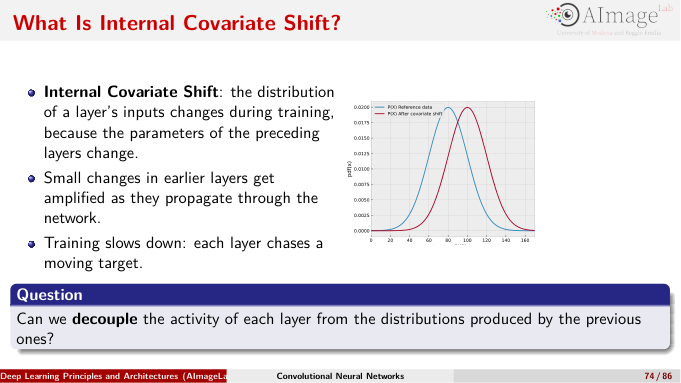
\includegraphics[keepaspectratio]{figure/fig_17875897a86c2eda.png}} \pandocbounded{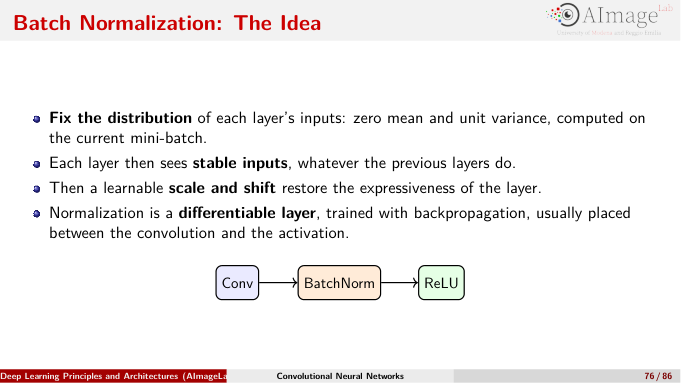
\includegraphics[keepaspectratio]{figure/fig_3598f417f405b2f8.png}}
% END F02-B0393

% BEGIN F02-B0394
La \textbf{Batch Normalization} standardizza con statistiche del mini-batch, poi applica scala e traslazione apprendibili. Nel blocco illustrato l\textquotesingle ordine è convoluzione → BatchNorm → ReLU. La stabilità delle distribuzioni è una motivazione: la trasformazione non rende immutabile l\textquotesingle intera distribuzione, indipendenti i livelli o gaussiani i valori.
% END F02-B0394

% BEGIN F02-B0395
\pandocbounded{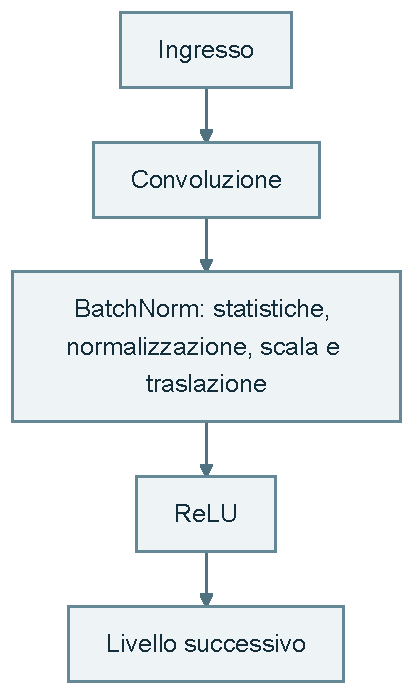
\includegraphics[keepaspectratio]{figure/diagramma_f02_10.pdf}}
% END F02-B0395

% BEGIN F02-B0396
\subsection{Formule e assi di aggregazione (slide 81--84)}\label{f02-r1155}
% END F02-B0396

% BEGIN F02-B0397
Sia \(X\in\mathbb{R}^{N\times C\times H\times W}\). Nelle CNN le statistiche sono calcolate \textbf{per canale}, aggregando batch e posizioni spaziali. Per ogni canale ci sono \(M=NHW\) valori. Media e varianza sono vettori in \(\mathbb{R}^C\), non una sola statistica per l\textquotesingle intero volume.
% END F02-B0397

% BEGIN F02-B0398
\begin{center}
\begin{adjustbox}{max width=\linewidth}
$\displaystyle 
\boxed{\begin{aligned}
\mu_{B,c}&=\frac1M\sum_{n=1}^N\sum_{h=1}^H\sum_{w=1}^W X_{n,c,h,w},\\
v_{B,c}&=\frac1M\sum_{n=1}^N\sum_{h=1}^H\sum_{w=1}^W(X_{n,c,h,w}-\mu_{B,c})^2,\\
\widehat X_{n,c,h,w}&=\frac{X_{n,c,h,w}-\mu_{B,c}}{\sqrt{v_{B,c}+\epsilon}},\\
Y_{n,c,h,w}&=\gamma_c\widehat X_{n,c,h,w}+\beta_c.
\end{aligned}}
$
\end{adjustbox}
\end{center}
% END F02-B0398

% BEGIN F02-B0399
\(\epsilon>0\) è una costante di stabilità; \(\gamma,\beta\in\mathbb{R}^C\) sono apprendibili. \(X,\widehat X,Y\) hanno la stessa forma. Le statistiche e i parametri vengono applicati mediante broadcasting a tutte le posizioni del rispettivo canale. Per un input denso \(N\times d\) si considera separatamente ogni feature, aggregando i \(N\) esempi.
% END F02-B0399

% BEGIN F02-B0400
\begin{figure}[H]
\centering
\pandocbounded{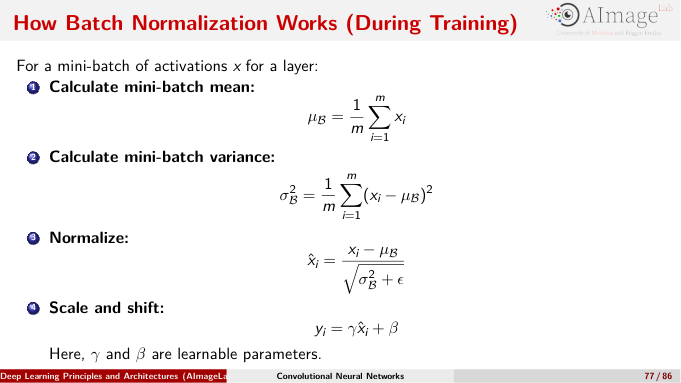
\includegraphics[keepaspectratio]{figure/fig_46e256c70ec88988.png}}
\caption{Slide 84 -- Quattro passaggi della Batch Normalization}
\end{figure}
% END F02-B0400

% BEGIN F02-B0401
La media è il centro aritmetico; sottrarla produce scarti con somma zero. La varianza è la media dei quadrati degli scarti e ha unità al quadrato. Per questo si divide per \textbf{la radice della varianza}, cioè la deviazione standard stabilizzata, non per la varianza.
% END F02-B0401

% BEGIN F02-B0402
Indicizzando i valori di un canale con \(a\):
% END F02-B0402

% BEGIN F02-B0403
\begin{center}
\begin{adjustbox}{max width=\linewidth}
$\displaystyle 
\begin{aligned}
\frac1M\sum_a(X_a-\mu_B)&=\frac1M\sum_aX_a-\mu_B=0,\\
\frac1M\sum_a\widehat X_a&=\frac{0}{\sqrt{v_B+\epsilon}}=0,\\
\frac1M\sum_a\widehat X_a^2&=\frac{\frac1M\sum_a(X_a-\mu_B)^2}{v_B+\epsilon}
=\frac{v_B}{v_B+\epsilon}.
\end{aligned}
$
\end{adjustbox}
\end{center}
% END F02-B0403

% BEGIN F02-B0404
La media normalizzata è zero; la varianza è vicina a 1 per \(v_B\gg\epsilon\), non esattamente 1. Se tutti i valori coincidono, \(v_B=0\) e le uscite normalizzate sono zero. Controllare questi due momenti non azzera le covarianze fra canali e non rende gaussiana la distribuzione.
% END F02-B0404

% BEGIN F02-B0405
\subsection{Esempio numerico completo (slide 81--85)}\label{f02-r1187}
% END F02-B0405

% BEGIN F02-B0406
Si prendano \(N=2,C=1,H=1,W=2\), quindi \(M=4\): le due mappe sono \([1,3]\) e \([5,7]\).
% END F02-B0406

% BEGIN F02-B0407
\begin{center}
\begin{adjustbox}{max width=\linewidth}
$\displaystyle 
\begin{aligned}
\mu_B&=(1+3+5+7)/4=4,\\
v_B&=\frac{(1-4)^2+(3-4)^2+(5-4)^2+(7-4)^2}{4}\\
&=(9+1+1+9)/4=5.
\end{aligned}
$
\end{adjustbox}
\end{center}
% END F02-B0407

% BEGIN F02-B0408
Con \(\epsilon=10^{-5}\), il denominatore è \(\sqrt{5.00001}\approx2.23607\) e
% END F02-B0408

% BEGIN F02-B0409
\begin{center}
\begin{adjustbox}{max width=\linewidth}
$\displaystyle \widehat X\approx(-1.34164,-0.44721,0.44721,1.34164).$
\end{adjustbox}
\end{center}
% END F02-B0409

% BEGIN F02-B0410
La varianza vale \(5/5.00001\approx0.999998\). Con \(\gamma=2,\beta=1\):
% END F02-B0410

% BEGIN F02-B0411
\begin{center}
\begin{adjustbox}{max width=\linewidth}
$\displaystyle \boxed{Y\approx(-1.68328,0.10557,1.89443,3.68328).}$
\end{adjustbox}
\end{center}
% END F02-B0411

% BEGIN F02-B0412
La forma rimane \(2\times1\times1\times2\). La media finale è 1, la varianza circa 4: la trasformazione affine non mantiene obbligatoriamente media zero e varianza unitaria.
% END F02-B0412

% BEGIN F02-B0413
\subsection{Perché apprendere gamma e beta? (slide 85)}\label{f02-r1209}
% END F02-B0413

% BEGIN F02-B0414
Una scala imposta permanentemente può limitare la rappresentazione. La normalizzazione fornisce una base controllata; \(\gamma_c\) e \(\beta_c\) scelgono scala e offset utili al compito.
% END F02-B0414

% BEGIN F02-B0415
\begin{center}
\begin{adjustbox}{max width=\linewidth}
$\displaystyle \boxed{\operatorname{media}_B(Y_c)=\beta_c,\qquad\operatorname{var}_B(Y_c)=\gamma_c^2\frac{v_{B,c}}{v_{B,c}+\epsilon}.}$
\end{adjustbox}
\end{center}
% END F02-B0415

% BEGIN F02-B0416
La prima relazione segue dalla linearità della media. La seconda deriva dal fatto che la traslazione non modifica gli scarti, mentre la moltiplicazione per \(\gamma\) ne moltiplica i quadrati per \(\gamma^2\). L\textquotesingle esempio con \(\gamma=2,\beta=1\) verifica entrambe.
% END F02-B0416

% BEGIN F02-B0417
A statistiche fissate, scegliere \(\gamma=\sqrt{v_B+\epsilon}\) e \(\beta=\mu_B\) ricostruisce l\textquotesingle ingresso:
% END F02-B0417

% BEGIN F02-B0418
\begin{center}
\begin{adjustbox}{max width=\linewidth}
$\displaystyle \gamma\frac{x-\mu_B}{\sqrt{v_B+\epsilon}}+\beta=(x-\mu_B)+\mu_B=x.$
\end{adjustbox}
\end{center}
% END F02-B0418

% BEGIN F02-B0419
Questo mostra la capacità di ripristinare la scala originale; due parametri fissi non invertono però esattamente ogni mini-batch se le sue statistiche cambiano.
% END F02-B0419

% BEGIN F02-B0420
Il numero dei parametri è
% END F02-B0420

% BEGIN F02-B0421
\begin{center}
\begin{adjustbox}{max width=\linewidth}
$\displaystyle \boxed{P_{\mathrm{BN}}=C+C=2C.}$
\end{adjustbox}
\end{center}
% END F02-B0421

% BEGIN F02-B0422
Con 64 canali si apprendono 128 scalari. Le statistiche mobili sono \textbf{stato del livello}, non parametri ottimizzati tramite gradient descent. Ponendo \(g_a=\partial\mathcal L/\partial Y_a\), la catena applicata a \(Y_a=\gamma\widehat X_a+\beta\) dà
% END F02-B0422

% BEGIN F02-B0423
\begin{center}
\begin{adjustbox}{max width=\linewidth}
$\displaystyle \boxed{\frac{\partial\mathcal L}{\partial\beta}=\sum_a g_a,\qquad\frac{\partial\mathcal L}{\partial\gamma}=\sum_a g_a\widehat X_a.}$
\end{adjustbox}
\end{center}
% END F02-B0423

% BEGIN F02-B0424
Si sommano i contributi perché gli stessi parametri sono condivisi dalle posizioni del canale. Con \(g=(1,0,0,0)\) nell\textquotesingle esempio, i gradienti sono 1 e circa \(-1.34164\).
% END F02-B0424

% BEGIN F02-B0425
\begin{figure}[H]
\centering
\pandocbounded{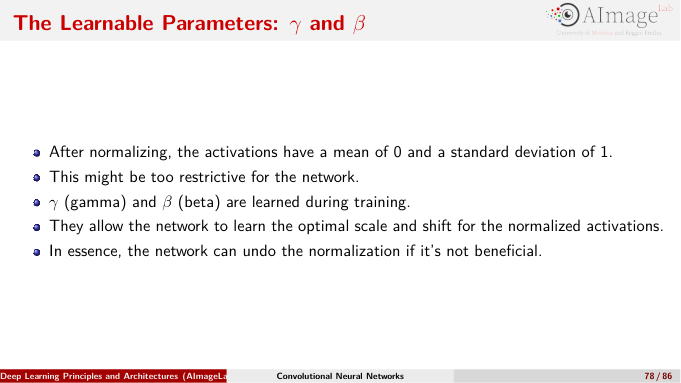
\includegraphics[keepaspectratio]{figure/fig_6c10410bff92bcbe.png}}
\caption{Slide 85 -- Parametri apprendibili gamma e beta}
\end{figure}
% END F02-B0425

% BEGIN F02-B0426
\subsection{Inferenza con statistiche memorizzate (slide 86)}\label{f02-r1235}
% END F02-B0426

% BEGIN F02-B0427
In training è disponibile un mini-batch; in inferenza può arrivare una sola immagine o un elemento di un flusso. Ricalcolare le statistiche renderebbe inoltre la predizione dipendente dagli altri esempi presenti nel batch di valutazione. Si conservano quindi statistiche durante il training e si riutilizzano dopo.
% END F02-B0427

% BEGIN F02-B0428
Con medie e varianze memorizzate \(\bar\mu,\bar v\in\mathbb{R}^C\):
% END F02-B0428

% BEGIN F02-B0429
\begin{center}
\begin{adjustbox}{max width=\linewidth}
$\displaystyle \boxed{Y_{n,c,h,w}=\gamma_c\frac{X_{n,c,h,w}-\bar\mu_c}{\sqrt{\bar v_c+\epsilon}}+\beta_c.}$
\end{adjustbox}
\end{center}
% END F02-B0429

% BEGIN F02-B0430
Si sostituiscono le statistiche correnti con quelle fissate dopo il training. A modello e ingresso fissati, questo livello non dipende dalla composizione del batch di inferenza. Con \(x=7\), \(\bar\mu=4\), \(\bar v=5\), \(\gamma=2\), \(\beta=1\) ed \(\epsilon=10^{-5}\), l\textquotesingle uscita è circa \(3.68328\).
% END F02-B0430

% BEGIN F02-B0431
Una media mobile esponenziale può aggiornare lo stato secondo
% END F02-B0431

% BEGIN F02-B0432
\begin{center}
\begin{adjustbox}{max width=\linewidth}
$\displaystyle \boxed{\begin{aligned}
\bar\mu_{t+1}&=(1-\rho)\bar\mu_t+\rho\mu_{B,t},\\
\bar v_{t+1}&=(1-\rho)\bar v_t+\rho\widetilde v_{B,t}.
\end{aligned}}$
\end{adjustbox}
\end{center}
% END F02-B0432

% BEGIN F02-B0433
\(0<\rho\leq1\) pesa la nuova osservazione e \(\widetilde v_B\) è la stima scelta per l\textquotesingle accumulatore. È una media pesata con coefficienti che sommano a 1. Con \(\rho=0.1\), media vecchia 2 e nuova osservazione 4 si ottiene \(0.9\cdot2+0.1\cdot4=2.2\). Con varianza vecchia 3 e nuova stima 5 si ottiene 3.2. La convenzione esatta dipende dall\textquotesingle implementazione: una media di varianze non coincide con il quadrato della media delle deviazioni standard.
% END F02-B0433

% BEGIN F02-B0434
\textbf{Un solo esempio non significa sempre un solo valore.} Per un unico scalare la varianza empirica con divisore 1 è definita e vale zero; quella corretta con divisore \(M-1\) non è definita per \(M=1\). Manca comunque informazione sulla dispersione della popolazione. Nella BatchNorm convoluzionale si aggregano \(M=NHW\) valori: anche con \(N=1\) possono esserci molti elementi spaziali. Usare statistiche fisse resta la procedura di inferenza discussa, ma non si giustifica affermando che ogni immagine singola abbia necessariamente varianza nulla.
% END F02-B0434

% BEGIN F02-B0435
\begin{figure}[H]
\centering
\pandocbounded{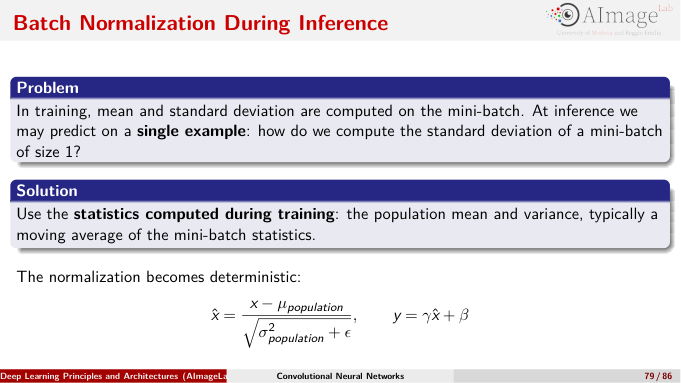
\includegraphics[keepaspectratio]{figure/fig_94728445c14605cb.png}}
\caption{Slide 86 -- Batch Normalization in inferenza}
\end{figure}
% END F02-B0435

% BEGIN F02-B0436
\subsection{Modalità training ed evaluation (slide 86 e chiusura della trascrizione)}\label{f02-r1258}
% END F02-B0436

% BEGIN F02-B0437
\begin{longtable}[]{@{}
  >{\raggedright\arraybackslash}p{(\linewidth - 4\tabcolsep) * \real{0.3333}}
  >{\raggedright\arraybackslash}p{(\linewidth - 4\tabcolsep) * \real{0.3333}}
  >{\raggedright\arraybackslash}p{(\linewidth - 4\tabcolsep) * \real{0.3333}}@{}}
\toprule\noalign{}
\begin{minipage}[b]{\linewidth}\raggedright
Livello
\end{minipage} & \begin{minipage}[b]{\linewidth}\raggedright
Training
\end{minipage} & \begin{minipage}[b]{\linewidth}\raggedright
Evaluation/inferenza
\end{minipage} \\
\midrule\noalign{}
\endhead
\bottomrule\noalign{}
\endlastfoot
BatchNorm con statistiche mobili & Usa il batch corrente e aggiorna lo stato & Usa le statistiche memorizzate \\
Dropout ordinario & Campiona una maschera che azzera alcune attivazioni & Non elimina casualmente le attivazioni \\
\end{longtable}
% END F02-B0437

% BEGIN F02-B0438
In PyTorch si usano \texttt{net.train()} e \texttt{net.eval()}. \texttt{net.training} è lo stato booleano, non la chiamata per impostarlo. Queste modalità governano i livelli; \texttt{eval()} non disabilita da solo il calcolo dei gradienti. Impostare correttamente la modalità è quindi necessario per valutare il comportamento previsto del modello.
% END F02-B0438

% BEGIN F02-B0439
\begin{quote}
\textbf{Stop-line verificata --- 08/10/2026}
\end{quote}
% END F02-B0439

% BEGIN F02-B0440
\begin{quote}
La trattazione termina alla \textbf{pagina PDF 86 di \texttt{03\_conv.pdf}}, ``Batch Normalization During Inference'', numerata \textbf{79/86} nel piè di pagina. La trascrizione si chiude con le statistiche di inferenza e il confronto BatchNorm/dropout nelle modalità training/eval. La successiva pagina PDF 87, ``Benefits of Batch Normalization'', non risulta spiegata nella registrazione e non viene sviluppata. Titoli e nomi delle immagini usano le pagine fisiche del PDF.
\end{quote}
% END F02-B0440

% BEGIN F02-B0441
\begin{center}\rule{0.5\linewidth}{0.5pt}\end{center}
% END F02-B0441

% BEGIN F02-B0442
\section{Riepilogo Formule Operative}\label{f02-r1273}
% END F02-B0442

% BEGIN F02-B0443
\begin{longtable}[]{@{}
  >{\raggedright\arraybackslash}p{(\linewidth - 4\tabcolsep) * \real{0.3333}}
  >{\raggedright\arraybackslash}p{(\linewidth - 4\tabcolsep) * \real{0.3333}}
  >{\raggedright\arraybackslash}p{(\linewidth - 4\tabcolsep) * \real{0.3333}}@{}}
\toprule\noalign{}
\begin{minipage}[b]{\linewidth}\raggedright
Concetto
\end{minipage} & \begin{minipage}[b]{\linewidth}\raggedright
Formula Matematica
\end{minipage} & \begin{minipage}[b]{\linewidth}\raggedright
Significato e Vincoli
\end{minipage} \\
\midrule\noalign{}
\endhead
\bottomrule\noalign{}
\endlastfoot
\textbf{Tensore Immagine RGB} & \(X \in \mathbb{R}^{C \times H \times W}\) & Standard PyTorch: \(C=3\) canali, \(H\) altezza, \(W\) larghezza \\
\textbf{Operatore LSI Discreto} & \(o(x, y) = \sum_m \sum_n i(m, n) K(x-m, y-n)\) & Convoluzione 2D con risposta all\textquotesingle impulso \(K\) \\
\textbf{Mappa di Feature Multicanale} & \(F(i, j) = b + \sum_{c=1}^{C_{in}} \sum_m \sum_n I(i+m, j+n, c) K_c(m, n)\) & Somma attraverso tutti i \(C_{in}\) canali di ingresso più bias scalare \(b\) \\
\textbf{Dimensioni Spaziali Uscita} & \(H' = \left\lfloor \frac{H - K + 2P}{S} \right\rfloor + 1, \; W' = \left\lfloor \frac{W - K + 2P}{S} \right\rfloor + 1\) & \(K\): kernel, \(P\): padding, \(S\): stride, \(\lfloor \cdot \rfloor\): floor \\
\textbf{Padding per Dimensione Costante ("same")} & \(P = \frac{K - 1}{2}\) & Valido per kernel dispari \(K\) con stride unitario \(S = 1\) \\
\textbf{Parametri Apprendibili Strato Conv} & \(\text{Parametri} = C_{out} \cdot (K^2 \cdot C_{in} + 1)\) & Completamente indipendente dalla risoluzione spaziale \(H \times W\) \\
\textbf{Attivazione ReLU} & \(f(x) = \max(0, x)\) & Gradiente 1 per \(x>0\); gradiente 0 per \(x<0\) (rischio dying ReLU) \\
\textbf{Attivazione Leaky ReLU} & \(f(x) = \max(x, \alpha x)\) & Pendenza \(\alpha \approx 0.01\) per \(x<0\) (mantiene vivo il gradiente) \\
\textbf{Attivazione ELU} & \(f(x) = x \text{ se } x>0, \; \alpha(e^x - 1) \text{ se } x \le 0\) & Asintoto a \(-\alpha\) per \(x \to -\infty\); media attivazioni vicina a 0 \\
\textbf{Pooling: forma, senza padding} & \(H'=\lfloor(H-K)/S\rfloor+1\), \(W'=\lfloor(W-K)/S\rfloor+1\) & \(N,C\) invariati; dilatazione 1, finestre compatibili \\
\textbf{Max pooling} & \(Y_{n,c,i,j}=\max_{u,v}X_{n,c,iS+u,jS+v}\) & \(0\leq u,v<K\); zero parametri apprendibili \\
\textbf{Average pooling} & \(Y_{n,c,i,j}=K^{-2}\sum_{u,v}X_{n,c,iS+u,jS+v}\) & Media sulla finestra; zero parametri apprendibili \\
\textbf{Global average pooling} & \(z_{n,c}=(hw)^{-1}\sum_{i,j}X_{n,c,i,j}\) & \(N\times C\times h\times w\to N\times C\times1\times1\) \\
\textbf{Pool adattivo a griglia fissa} & \(N\times C\times h\times w\to N\times C\times o\times o\) & Dopo flatten: \(Co^2\) ingressi per esempio \\
\textbf{Campo recettivo} & \(r_\ell=r_{\ell-1}+(k_\ell-1)j_{\ell-1}\), \(j_\ell=s_\ell j_{\ell-1}\) & \(r_0=j_0=1\), senza dilatazione \\
\textbf{Parametri dense} & \(d_{\mathrm{out}}(d_{\mathrm{in}}+1)\) & Bias incluso \\
\textbf{Blocco residuo} & \(H=x+F(x)\) & Stesse forme; entrambi i rami calcolati \\
\textbf{Gradiente residuo} & \(\nabla_x\mathcal L=g+J_F^Tg\) & Somma, non selezione, dei contributi \\
\textbf{BN: media e varianza} & \(\mu_{B,c}=M^{-1}\sum_aX_{a,c}\), \(v_{B,c}=M^{-1}\sum_a(X_{a,c}-\mu_{B,c})^2\) & \(M=NHW\), una coppia per canale \\
\textbf{BN: training} & \(Y_c=\gamma_c(X_c-\mu_{B,c})/\sqrt{v_{B,c}+\epsilon}+\beta_c\) & Forma invariata; \(2C\) parametri apprendibili \\
\textbf{BN: inferenza} & \(Y_c=\gamma_c(X_c-\bar\mu_c)/\sqrt{\bar v_c+\epsilon}+\beta_c\) & Statistiche memorizzate; nessun nuovo calcolo sul batch \\
\end{longtable}
% END F02-B0443

% BEGIN F02-B0444
\section{Errata e precisazioni principali}\label{f02-r1299}
% END F02-B0444

% BEGIN F02-B0445
\begin{longtable}[]{@{}
  >{\raggedright\arraybackslash}p{(\linewidth - 2\tabcolsep) * \real{0.5000}}
  >{\raggedright\arraybackslash}p{(\linewidth - 2\tabcolsep) * \real{0.5000}}@{}}
\toprule\noalign{}
\begin{minipage}[b]{\linewidth}\raggedright
Riferimento
\end{minipage} & \begin{minipage}[b]{\linewidth}\raggedright
Precisazione
\end{minipage} \\
\midrule\noalign{}
\endhead
\bottomrule\noalign{}
\endlastfoot
Slide 25 & Linearità significa sovrapposizione dei segnali, non movimento rettilineo della finestra. \\
Slide 32 e spiegazione orale & Convoluzione e correlazione differiscono per il ribaltamento del kernel, non per la scelta del centro dell\textquotesingle uscita. \\
Slide 38 & Il campo recettivo teorico cresce componendo regioni; due kernel \(3\times3\) a stride 1 danno \(5\times5\). \\
Slide 54 & Una ReLU negativa non blocca l\textquotesingle intero modello; ELU è differenziabile in zero solo per \(\alpha=1\). \\
Slide 55--57 & Il dimezzamento dei due assi richiede \(K=S=2\) nell\textquotesingle esempio; pooling non cambia i canali. \\
Slide 59 & Il pooling adattivo precede flattening e MLP; non li sostituisce entrambi. \\
Slide 65--66 & Le ReLU dei livelli nascosti sono distinte dall\textquotesingle uscita finale di classificazione. \\
Slide 71--74 & Shortcut identità solo a forme coincidenti; i rami e i gradienti vengono sommati. \\
Slide 80--85 & BN non impone gaussianità né decorrelazione; con \(\epsilon>0\) la varianza normalizzata non è esattamente 1. \\
Slide 86 & Nelle CNN \(N=1\) non implica \(NHW=1\); \texttt{train()}/\texttt{eval()} cambiano la modalità dei livelli. \\
\end{longtable}
% END F02-B0445


% BEGIN F03-B0001
\chapter{RNN - Reti neurali ricorrenti}\label{fonte03}
% END F03-B0001

% BEGIN F03-B0002
\begin{indiceargomento}
\item \hyperref[f03-r34]{Serie temporali e sequenze di lunghezza variabile (slide 3--4)}
\item \hyperref[f03-r66]{Pattern temporali: trend, stagionalità e residuo (slide 5--8)}
\item \hyperref[f03-r106]{Forecasting: continuare una sequenza (slide 9--12)}
\item \hyperref[f03-r139]{Autoregressione e richiamo ai modelli statistici (slide 13--14)}
\item \hyperref[f03-r172]{Preparazione dei dati e codifica ciclica (slide 15--18)}
\item \hyperref[f03-r230]{Reti ricorrenti e forme dei problemi sequenziali (slide 19--21)}
\item \hyperref[f03-r248]{Vanilla RNN: equazioni, dimensioni e significato (slide 22)}
\item \hyperref[f03-r346]{Hidden state: un riassunto utile, non il modello appreso (slide 23)}
\item \hyperref[f03-r384]{Unfolding: esplicitare il calcolo nel tempo (slide 24--26)}
\item \hyperref[f03-r410]{BPTT: sommare i contributi ai parametri condivisi (slide 27)}
\item \hyperref[f03-r547]{Dipendenze a lungo termine e instabilità del gradiente (slide 28--29)}
\item \hyperref[f03-r638]{Memoria selettiva e architetture con gate (slide 30)}
\item \hyperref[f03-r648]{LSTM: stato interno e quadro delle equazioni (slide 31)}
\item \hyperref[f03-r687]{Gate: interruttori continui apprendibili (slide 32)}
\item \hyperref[f03-r741]{Stato candidato: proporre un nuovo contenuto (slide 33)}
\item \hyperref[f03-r762]{Aggiornare la memoria ed esporre lo stato (slide 34)}
\item \hyperref[f03-r838]{Perché separare cell state e hidden state (slide 35)}
\item \hyperref[f03-r874]{Riepilogo operativo (slide 4--35)}
\item \hyperref[f03-r898]{Errata e precisazioni da conservare nel ripasso (slide 4--35)}
\end{indiceargomento}
% END F03-B0002

% BEGIN F03-B0003
Le reti convoluzionali sfruttano la struttura spaziale delle immagini. Le \textbf{reti neurali ricorrenti}, o \textbf{RNN}, sfruttano invece l\textquotesingle ordine di una sequenza: a ogni passo combinano una nuova osservazione con una rappresentazione di quanto è stato elaborato prima. Il problema centrale è costruire e apprendere una memoria utile al compito, anche quando le sequenze hanno lunghezze diverse.
% END F03-B0003

% BEGIN F03-B0004
\pandocbounded{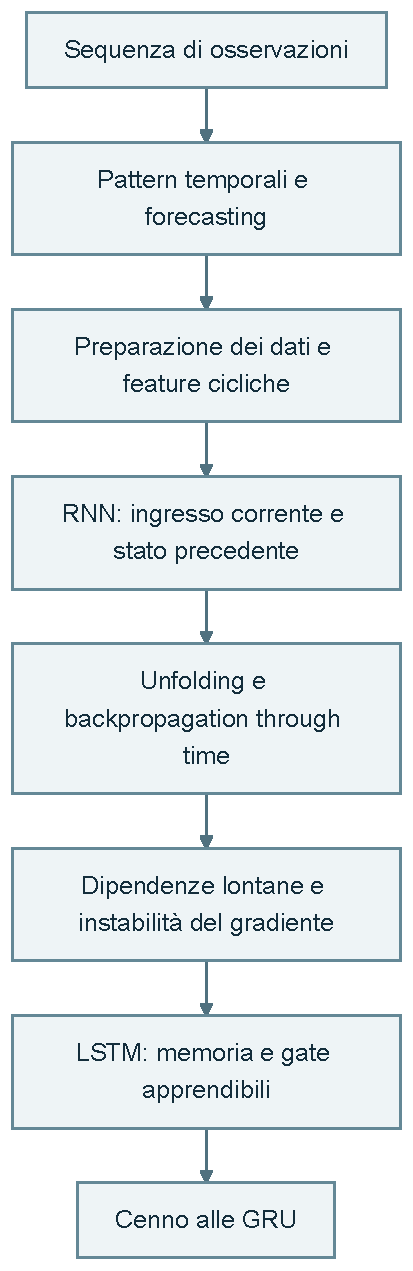
\includegraphics[keepaspectratio]{figure/diagramma_f03_01.pdf}}
% END F03-B0004

% BEGIN F03-B0005
\section{Serie temporali e sequenze di lunghezza variabile (slide 3--4)}\label{f03-r34}
% END F03-B0005

% BEGIN F03-B0006
Una \textbf{serie temporale} è una successione ordinata di osservazioni raccolte nel tempo. Esempi sono un segnale audio o una canzone, la temperatura misurata giorno per giorno, il prezzo di un titolo finanziario e le misure di un sensore. L\textquotesingle ordine è parte dell\textquotesingle informazione: scambiare due osservazioni può modificare il significato della sequenza.
% END F03-B0006

% BEGIN F03-B0007
Si distinguono un tempo continuo, in cui il segnale è definito su un intervallo temporale, e un tempo discreto, in cui si considerano istanti separati. Qui si lavora con sequenze discrete osservate per un numero finito di passi:
% END F03-B0007

% BEGIN F03-B0008
\begin{center}
\begin{adjustbox}{max width=\linewidth}
$\displaystyle \boxed{X=(x_1,x_2,\ldots,x_T),\qquad x_t\in\mathbb R^d.}$
\end{adjustbox}
\end{center}
% END F03-B0008

% BEGIN F03-B0009
\(T\) è la \textbf{lunghezza della sequenza}; \(d\) è il \textbf{numero di feature di ogni osservazione}. Con vettori colonna, ogni \(x_t\) ha forma \(d\times1\). Disporre una osservazione per riga produce una rappresentazione tabellare \(X\in\mathbb R^{T\times d}\).
% END F03-B0009

% BEGIN F03-B0010
\begin{itemize}
\tightlist
\item
  Una serie \textbf{univariata} ha \(d=1\): per esempio il solo numero di passeggeri.
\item
  Una serie \textbf{multivariata} ha \(d>1\): per esempio più misure meteorologiche per ciascun giorno. Aggiungere una codifica della data alle misure aumenta il numero di feature.
\end{itemize}
% END F03-B0010

% BEGIN F03-B0011
La differenza fra una e più componenti è analoga a quella fra un valore grayscale e i tre canali RGB di \hyperref[fonte02]{reti convoluzionali}; un\textquotesingle immagine RGB isolata, però, non è per questo una serie temporale. Una successione di immagini, come un video, possiede anche l\textquotesingle asse temporale. Analogamente, una nuvola di punti LiDAR isolata è un insieme spaziale, mentre misure LiDAR successive possono formare una sequenza.
% END F03-B0011

% BEGIN F03-B0012
Se il campionamento è regolare, gli istanti soddisfano
% END F03-B0012

% BEGIN F03-B0013
\begin{center}
\begin{adjustbox}{max width=\linewidth}
$\displaystyle \boxed{t_k=t_0+k\Delta t,\qquad f_c=\frac1{\Delta t}.}$
\end{adjustbox}
\end{center}
% END F03-B0013

% BEGIN F03-B0014
Il primo istante è \(t_0\) e ogni passo aggiunge lo stesso intervallo \(\Delta t\). In un secondo entrano \(1/\Delta t\) intervalli, da cui la frequenza di campionamento \(f_c\). Per esempio, una misura ogni \(0.5\) secondi corrisponde a \(f_c=2\) Hz. Per dati mensili il passo è invece un mese: si usa l\textquotesingle unità temporale appropriata.
% END F03-B0014

% BEGIN F03-B0015
\begin{quote}
\textbf{Errata slide 4 --- Discreto non significa finito}
\end{quote}
% END F03-B0015

% BEGIN F03-B0016
\begin{quote}
Il tempo discreto è definito dall\textquotesingle insieme separato degli indici, non dalla finitezza della serie. Una serie discreta può continuare indefinitamente; è il campione osservato nel dataset a essere finito. Il campionamento regolare richiede inoltre un intervallo costante, non soltanto osservazioni discrete.
\end{quote}
% END F03-B0016

% BEGIN F03-B0017
\subsection{Sequenze di parole e limite dell\textquotesingle ingresso fisso (slide 4)}\label{f03-r58}
% END F03-B0017

% BEGIN F03-B0018
Una frase è una sequenza in cui l\textquotesingle indice \(t\) indica la posizione, senza dover rappresentare un tempo fisico. Ogni elemento può essere un token, identificato da un indice in un vocabolario e fornito alla rete mediante una rappresentazione numerica. Due frasi possono contenere numeri diversi di token.
% END F03-B0018

% BEGIN F03-B0019
Per classificare il sentiment di una frase, un MLP applicato direttamente alla concatenazione degli ingressi richiede una dimensione iniziale fissata. Con \(T\) osservazioni di \(d\) feature, la concatenazione ha \(Td\) componenti: se \(T\) cambia, cambia anche il numero di ingressi richiesto al primo livello denso. È la stessa rigidità della testa densa discussa in \hyperref[fonte02]{reti convoluzionali}.
% END F03-B0019

% BEGIN F03-B0020
Non significa che un MLP non possa mai essere usato con dati temporali: finestre e rappresentazioni di lunghezza fissata sono possibili. La RNN affronta direttamente il problema riutilizzando \textbf{lo stesso aggiornamento per ogni elemento}, per quante osservazioni siano presenti. Può variare \(T\), mentre la dimensione \(d\) dell\textquotesingle osservazione e quella dello stato rimangono fissate dal modello.
% END F03-B0020

% BEGIN F03-B0021
\section{Pattern temporali: trend, stagionalità e residuo (slide 5--8)}\label{f03-r66}
% END F03-B0021

% BEGIN F03-B0022
Il grafico dei passeggeri aerei internazionali contiene misure mensili espresse in migliaia. Mostra contemporaneamente due regolarità: picchi che tendono a ripetersi e un livello complessivo che cresce. La prima suggerisce una componente stagionale; la seconda un trend crescente. Le annotazioni della slide evidenziano proprio la coesistenza delle due componenti.
% END F03-B0022

% BEGIN F03-B0023
\begin{figure}[H]
\centering
\pandocbounded{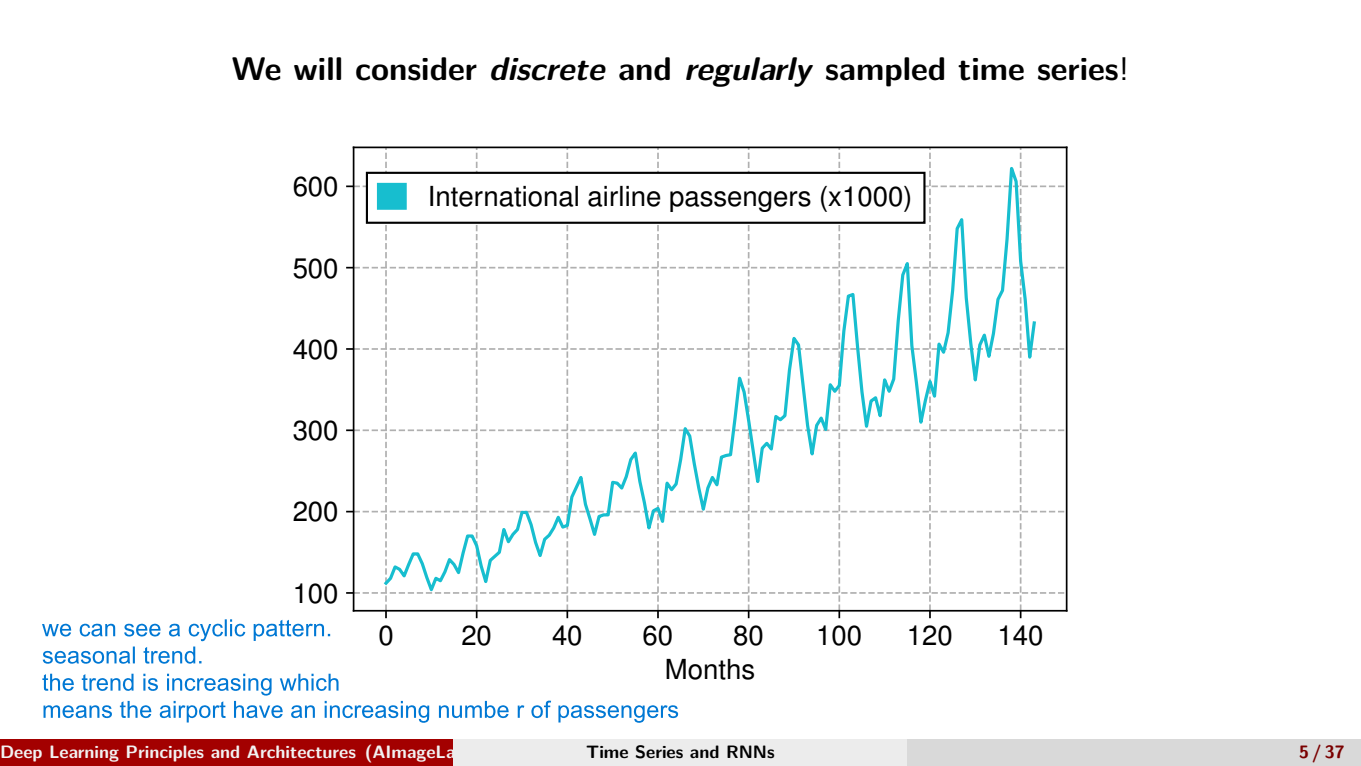
\includegraphics[keepaspectratio]{figure/fig_f22301011c2de1ca.png}}
\caption{Slide 5 --- Serie dei passeggeri con annotazioni su periodicità e trend}
\end{figure}
% END F03-B0023

% BEGIN F03-B0024
\begin{longtable}[]{@{}
  >{\raggedright\arraybackslash}p{(\linewidth - 4\tabcolsep) * \real{0.3333}}
  >{\raggedright\arraybackslash}p{(\linewidth - 4\tabcolsep) * \real{0.3333}}
  >{\raggedright\arraybackslash}p{(\linewidth - 4\tabcolsep) * \real{0.3333}}@{}}
\toprule\noalign{}
\begin{minipage}[b]{\linewidth}\raggedright
Componente
\end{minipage} & \begin{minipage}[b]{\linewidth}\raggedright
Significato
\end{minipage} & \begin{minipage}[b]{\linewidth}\raggedright
Lettura dell\textquotesingle esempio
\end{minipage} \\
\midrule\noalign{}
\endhead
\bottomrule\noalign{}
\endlastfoot
\textbf{Trend} & Tendenza di fondo verso valori più alti o più bassi & Il numero di passeggeri cresce negli anni \\
\textbf{Stagionalità} & Fluttuazione che si ripete secondo un periodo di riferimento & Mesi corrispondenti tendono a mostrare comportamenti ricorrenti \\
\textbf{Ciclo} & Oscillazione attorno al trend & Una variazione ricorrente, non necessariamente legata a un calendario rigidamente fissato \\
\textbf{Outlier} & Osservazione insolita rispetto al comportamento atteso & Un valore eccezionalmente alto o basso, da interpretare nel suo contesto \\
\textbf{Residuo} & Parte non spiegata dalle componenti considerate & Rumore, irregolarità e pattern rimasti fuori dalla decomposizione \\
\end{longtable}
% END F03-B0024

% BEGIN F03-B0025
Le misure possono contenere rumore di acquisizione; inoltre, l\textquotesingle evoluzione reale può dipendere da fattori non osservati. Nei dati finanziari, per esempio, molte cause influenzano il prezzo. Una componente stocastica non implica soltanto un sensore impreciso: può descrivere anche incertezza del processo o fattori non modellati.
% END F03-B0025

% BEGIN F03-B0026
Una scomposizione additiva permette di leggere il grafico come
% END F03-B0026

% BEGIN F03-B0027
\begin{center}
\begin{adjustbox}{max width=\linewidth}
$\displaystyle \boxed{x_t=a_t+s_t+r_t,}$
\end{adjustbox}
\end{center}
% END F03-B0027

% BEGIN F03-B0028
dove \(a_t\) è il trend, \(s_t\) la stagionalità e \(r_t\) il residuo, tutti scalari con le stesse unità di \(x_t\). Si ottiene il residuo sottraendo le parti spiegate:
% END F03-B0028

% BEGIN F03-B0029
\begin{center}
\begin{adjustbox}{max width=\linewidth}
$\displaystyle 
\begin{aligned}
x_t&=a_t+s_t+r_t &&\text{somma delle componenti},\\
x_t-a_t-s_t&=r_t &&\text{sottrazione di trend e stagionalità}.
\end{aligned}
$
\end{adjustbox}
\end{center}
% END F03-B0029

% BEGIN F03-B0030
Se in un mese si osservano 135 migliaia di passeggeri, con trend stimato 120 e componente stagionale 10, il residuo è \(135-120-10=5\). La ricostruzione trend più stagionalità vale 130; la differenza di 5 è ciò che quella ricostruzione non descrive. Non è automaticamente rumore bianco.
% END F03-B0030

% BEGIN F03-B0031
\begin{figure}[H]
\centering
\pandocbounded{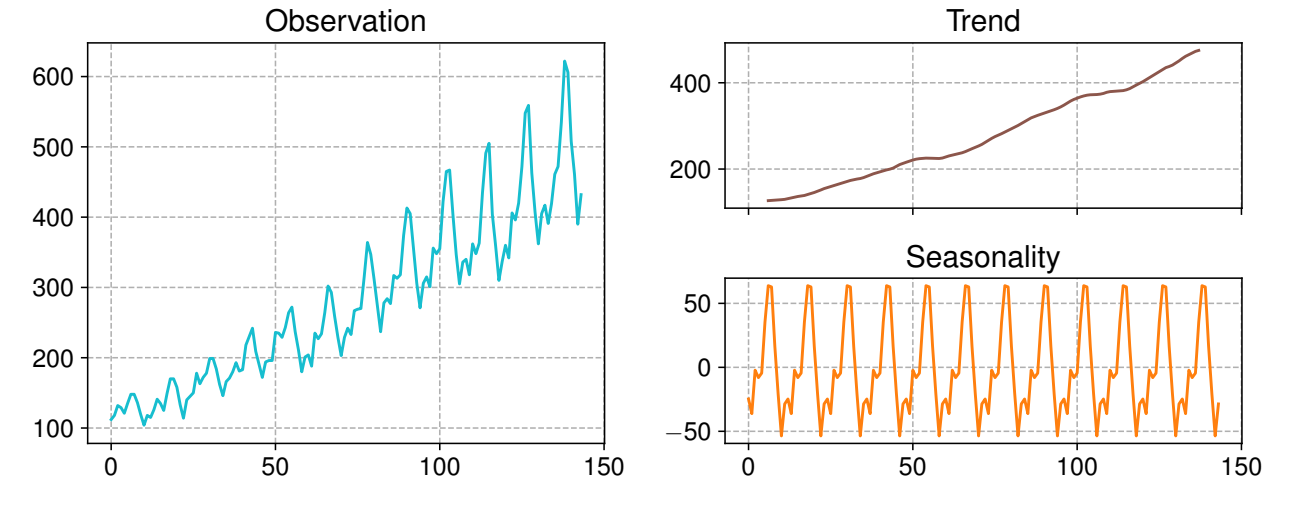
\includegraphics[keepaspectratio]{figure/fig_762a5612ce759898.png}}
\caption{Slide 7 --- Osservazione, trend e componente stagionale}
\end{figure}
% END F03-B0031

% BEGIN F03-B0032
\begin{figure}[H]
\centering
\pandocbounded{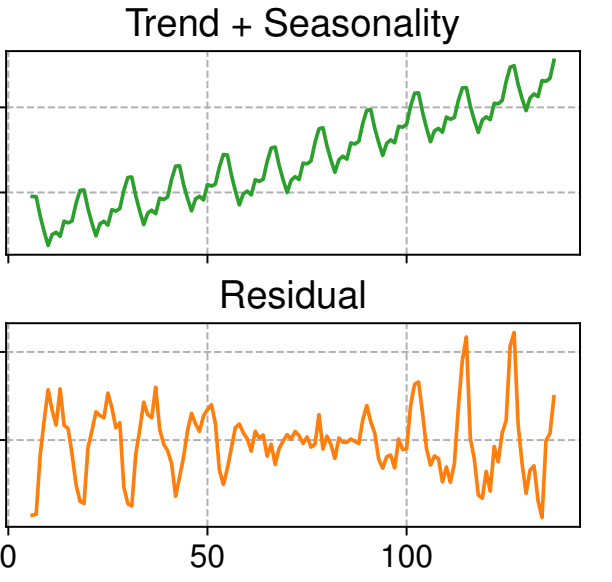
\includegraphics[keepaspectratio]{figure/fig_9adbce5099a492af.png}}
\caption{Slide 8 --- Somma delle componenti e residuo}
\end{figure}
% END F03-B0032

% BEGIN F03-B0033
La \textbf{stazionarietà} descrive proprietà statistiche che non cambiano nel tempo. Una media che aumenta con il trend è già sufficiente a escludere la stazionarietà. Media e varianza costanti, da sole, non esauriscono tutte le condizioni: per la stazionarietà debole anche la covarianza deve dipendere dalla distanza temporale, non dall\textquotesingle istante assoluto. Qui il concetto serve a leggere i dati, senza introdurre test o procedure di stazionarizzazione.
% END F03-B0033

% BEGIN F03-B0034
\begin{quote}
\textbf{Slide 6--8 --- Formalizzazione presente nelle slide, non approfondita}
\end{quote}
% END F03-B0034

% BEGIN F03-B0035
\begin{quote}
Le slide nominano la decomposizione \textbf{STL}, basata su regressione LOESS per separare trend e stagionalità, e la definizione di stazionarietà. La lettura qualitativa dei pattern è centrale; l\textquotesingle algoritmo LOESS, i test statistici e i dettagli della procedura STL non sono sviluppati e non vengono aggiunti.
\end{quote}
% END F03-B0035

% BEGIN F03-B0036
\section{Forecasting: continuare una sequenza (slide 9--12)}\label{f03-r106}
% END F03-B0036

% BEGIN F03-B0037
Il \textbf{forecasting} consiste nel prevedere valori futuri usando osservazioni disponibili fino a un certo istante. Indichiamo con \(T\) l\textquotesingle ultimo passo osservato e con \(h>0\) l\textquotesingle{}\textbf{orizzonte di previsione}:
% END F03-B0037

% BEGIN F03-B0038
\begin{center}
\begin{adjustbox}{max width=\linewidth}
$\displaystyle \boxed{\widehat x_{T+h}=F_\theta(x_1,\ldots,x_T;h).}$
\end{adjustbox}
\end{center}
% END F03-B0038

% BEGIN F03-B0039
\(F_\theta\) è il modello con parametri \(\theta\); \(\widehat x_{T+h}\) è la stima della futura osservazione. Nel caso multivariato appartiene a \(\mathbb R^d\), come \(x_t\). Per ottenere più passi si può considerare il vettore delle previsioni da \(T+1\) a \(T+H\).
% END F03-B0039

% BEGIN F03-B0040
La costruzione del problema avviene in tre passaggi: si sceglie dove terminano i dati osservati; si decide quanto avanti guardare; si confronta la previsione con il valore futuro effettivamente osservato. Per esempio, osservando i valori mensili \((100,110,120)\), una prosecuzione illustrativa della crescita di 10 al mese darebbe 130 a orizzonte 1 e 140 a orizzonte 2. È una possibile previsione, non una conseguenza certa dei tre numeri.
% END F03-B0040

% BEGIN F03-B0041
Tra le applicazioni ci sono la previsione della traiettoria di un veicolo, della domanda elettrica, della domanda di prodotti e dei valori finanziari. Prevedere la domanda permette di preparare l\textquotesingle offerta; prevedere una traiettoria aiuta ad anticipare dove si troverà un oggetto.
% END F03-B0041

% BEGIN F03-B0042
\subsection{Previsione puntuale e incertezza (slide 10--11)}\label{f03-r118}
% END F03-B0042

% BEGIN F03-B0043
La linea tratteggiata nella figura rappresenta una possibile previsione puntuale. La fascia attorno alla linea esprime invece un intervallo di valori plausibili. Nell\textquotesingle esempio la fascia si allarga all\textquotesingle aumentare dell\textquotesingle orizzonte: più ci si allontana dalle osservazioni, maggiore è l\textquotesingle incertezza rappresentata.
% END F03-B0043

% BEGIN F03-B0044
\begin{figure}[H]
\centering
\pandocbounded{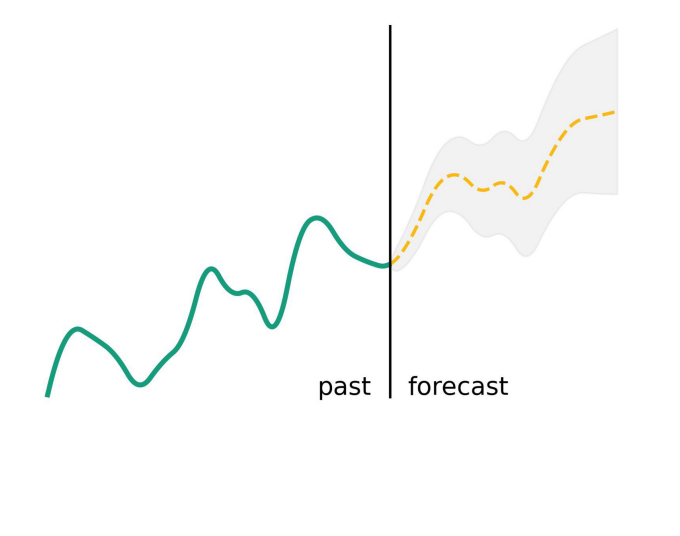
\includegraphics[keepaspectratio]{figure/fig_2e8b6609ad5f75ec.png}}
\caption{Slide 11 --- Passato osservato, previsione e fascia di incertezza}
\end{figure}
% END F03-B0044

% BEGIN F03-B0045
Un intervallo dichiarato al 90\% mira a contenere il valore futuro con quella copertura, sotto le ipotesi e la calibrazione del metodo. Per esempio, una previsione 130 accompagnata dall\textquotesingle intervallo \([120,140]\) comunica sia un valore centrale sia la sua incertezza. La sola presenza di una fascia nel disegno non dimostra la copertura del 90\%, né impone una distribuzione gaussiana. La costruzione di tali intervalli non viene sviluppata qui.
% END F03-B0045

% BEGIN F03-B0046
\begin{quote}
\textbf{Errata slide 10 --- Conoscere il processo non elimina il caso}
\end{quote}
% END F03-B0046

% BEGIN F03-B0047
\begin{quote}
Conoscere il processo generatore dei dati permette di descrivere correttamente la distribuzione futura; non garantisce di prevedere perfettamente ogni realizzazione se rimangono innovazioni casuali. Una previsione esatta a ogni orizzonte richiederebbe anche assenza di imprevedibilità residua e disponibilità delle informazioni necessarie.
\end{quote}
% END F03-B0047

% BEGIN F03-B0048
\subsection{Finestre di osservazione e componente casuale (slide 12)}\label{f03-r129}
% END F03-B0048

% BEGIN F03-B0049
Spesso la previsione usa una finestra limitata di osservazioni precedenti. Per prevedere il passo \(t\) a partire da \(q\) ritardi, l\textquotesingle ingresso è \((x_{t-1},\ldots,x_{t-q})\): sono \(q\) osservazioni. La funzione appresa cerca di sfruttare le relazioni temporali contenute in quella finestra.
% END F03-B0049

% BEGIN F03-B0050
\begin{quote}
\textbf{Slide 12 --- Schema statistico generale non sviluppato}
\end{quote}
% END F03-B0050

% BEGIN F03-B0051
\begin{quote}
La slide scrive \(x_t=f(x_{t-1},\ldots,x_{t-q};\phi)+g(\xi_{t-1},\ldots,\xi_{t-q};\theta)\), separando una funzione dei valori passati da una dei disturbi. \(\phi,\theta\) sono parametri e \(\xi\) indica disturbi casuali. È una rappresentazione introduttiva, non l\textquotesingle equazione della RNN né una definizione universale dei modelli di forecasting. Non si sviluppano qui stima dei disturbi o modelli combinati.
\end{quote}
% END F03-B0051

% BEGIN F03-B0052
\begin{quote}
\textbf{Errata slide 12 --- Indici della finestra}
\end{quote}
% END F03-B0052

% BEGIN F03-B0053
\begin{quote}
L\textquotesingle insieme \(\{x_t,\ldots,x_{t-q}\}\) riportato nel testo contiene \(q+1\) osservazioni e include il valore da prevedere nella formula sottostante. Per prevedere \(x_t\) con \(q\) soli valori passati si usa \(\{x_{t-1},\ldots,x_{t-q}\}\). Inoltre lo schema dei disturbi non esplicita un\textquotesingle innovazione corrente \(\xi_t\): non va letto come un modello stocastico completo senza ulteriori ipotesi.
\end{quote}
% END F03-B0053

% BEGIN F03-B0054
\section{Autoregressione e richiamo ai modelli statistici (slide 13--14)}\label{f03-r139}
% END F03-B0054

% BEGIN F03-B0055
Un modello è \textbf{autoregressivo} quando descrive un valore attraverso i valori precedenti della stessa sequenza. Nel modello lineare AR di ordine \(p\):
% END F03-B0055

% BEGIN F03-B0056
\begin{center}
\begin{adjustbox}{max width=\linewidth}
$\displaystyle \boxed{x_t=\sum_{i=1}^{p}\phi_i x_{t-i}+\xi_t.}$
\end{adjustbox}
\end{center}
% END F03-B0056

% BEGIN F03-B0057
Qui \(x_t,x_{t-i},\xi_t\) sono scalari; \(\phi=(\phi_1,\ldots,\phi_p)\in\mathbb R^p\) contiene i coefficienti da stimare. Il termine \(\xi_t\) rappresenta un\textquotesingle innovazione a media zero. Il rumore bianco ha assenza di correlazione fra istanti distinti; la gaussianità è una possibile ipotesi aggiuntiva, non la sua definizione.
% END F03-B0057

% BEGIN F03-B0058
L\textquotesingle equazione nasce scegliendo una combinazione lineare di \(p\) ritardi e aggiungendo ciò che non è previsto da quella combinazione. Con \(p=2\):
% END F03-B0058

% BEGIN F03-B0059
\begin{center}
\begin{adjustbox}{max width=\linewidth}
$\displaystyle 
\begin{aligned}
x_t&=\phi_1x_{t-1}+\phi_2x_{t-2}+\xi_t &&\text{sviluppo della somma},\\
\widehat x_t&=\phi_1x_{t-1}+\phi_2x_{t-2} &&\text{previsione con innovazione a media condizionale zero}.
\end{aligned}
$
\end{adjustbox}
\end{center}
% END F03-B0059

% BEGIN F03-B0060
Con coefficienti \(0.6\) e \(0.2\) e osservazioni precedenti 120 e 100:
% END F03-B0060

% BEGIN F03-B0061
\begin{center}
\begin{adjustbox}{max width=\linewidth}
$\displaystyle \widehat x_t=0.6\cdot120+0.2\cdot100=72+20=92.$
\end{adjustbox}
\end{center}
% END F03-B0061

% BEGIN F03-B0062
Se l\textquotesingle innovazione realizzata è 3, il valore osservato è 95. La differenza rende concreta la distinzione fra previsione e osservazione. L\textquotesingle equazione mostrata omette l\textquotesingle intercetta; una trasformazione affine può includere anche un termine costante.
% END F03-B0062

% BEGIN F03-B0063
\begin{figure}[H]
\centering
\pandocbounded{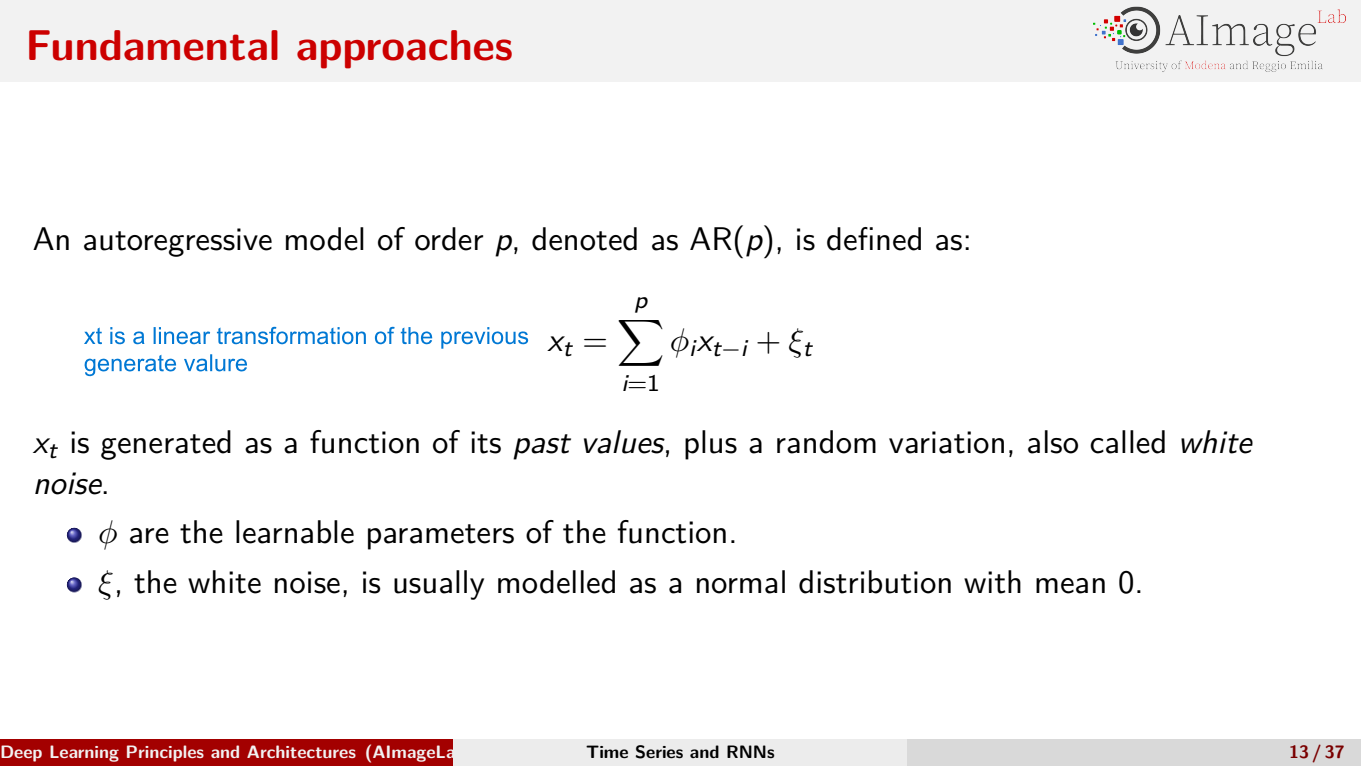
\includegraphics[keepaspectratio]{figure/fig_c490ed9c25c37069.png}}
\caption{Slide 13 --- Modello AR e annotazione sulla dipendenza dai valori precedenti}
\end{figure}
% END F03-B0063

% BEGIN F03-B0064
Il principio autoregressivo ricompare nella generazione di testo: il nuovo token è condizionato al contesto già disponibile, compresi i token generati prima. Questo non rende un generatore linguistico un modello AR lineare: il principio di condizionamento è condiviso, la funzione che lo realizza può essere non lineare.
% END F03-B0064

% BEGIN F03-B0065
\begin{quote}
\textbf{Slide 14 --- Moving Average, presente nelle slide ma non sviluppato}
\end{quote}
% END F03-B0065

% BEGIN F03-B0066
\begin{quote}
Il modello MA di ordine \(q\) è riportato come \(x_t=\mu+\xi_t+\sum_{i=1}^q\theta_i\xi_{t-i}\): combina innovazione corrente e innovazioni precedenti mediante coefficienti \(\theta_i\). Qui \(\mu\) è la media teorica del processo quando i disturbi hanno media zero; la media empirica può stimarla, ma non coincide per definizione con essa. Non è una media mobile dei valori osservati. Stima e applicazioni del modello MA non sono state sviluppate.
\end{quote}
% END F03-B0066

% BEGIN F03-B0067
\begin{quote}
\textbf{Errata slide 14 --- Media del processo e media campionaria}
\end{quote}
% END F03-B0067

% BEGIN F03-B0068
\begin{quote}
Identificare direttamente il parametro \(\mu\) con la media empirica confonde una quantità del modello con un suo possibile stimatore. Sono concetti distinti anche se la seconda viene usata per stimare la prima.
\end{quote}
% END F03-B0068

% BEGIN F03-B0069
\section{Preparazione dei dati e codifica ciclica (slide 15--18)}\label{f03-r172}
% END F03-B0069

% BEGIN F03-B0070
Preparare una serie richiede di distinguere il \textbf{valore osservato} dall\textquotesingle{}\textbf{informazione temporale} associata. Una stringa come \texttt{1949-01} deve essere interpretata come una data, non come una generica etichetta: anno e mese possono essere estratti per organizzare e rappresentare le osservazioni. Le prime righe mostrate nelle slide associano, per esempio, gennaio 1949 a 112 migliaia di passeggeri e febbraio a 118.
% END F03-B0070

% BEGIN F03-B0071
Una seconda scelta riguarda la rappresentazione del segnale. Nel \textbf{dominio del tempo} si mantengono le osservazioni ordinate; nel \textbf{dominio delle frequenze} si descrivono componenti oscillatorie, per esempio mediante Fourier. Per vibrazioni di motori, le componenti in frequenza possono essere informative. Le reti ricorrenti qui descritte lavorano sugli ingressi nel dominio del tempo, senza richiedere una trasformata di Fourier preliminare.
% END F03-B0071

% BEGIN F03-B0072
\begin{figure}[H]
\centering
\pandocbounded{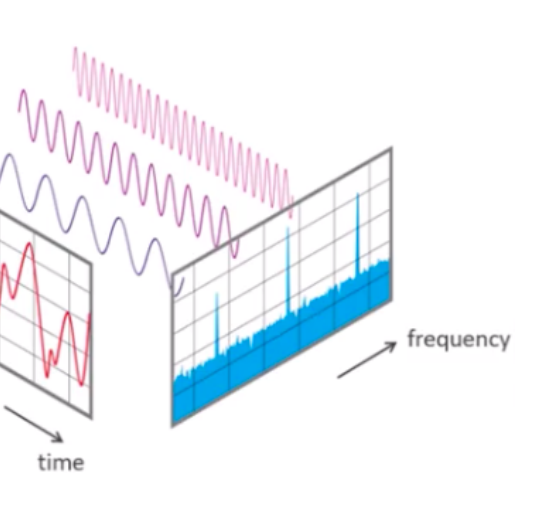
\includegraphics[keepaspectratio]{figure/fig_1b37f2cd21254e9d.png}}
\caption{Slide 16 --- Rappresentazione nel tempo e nelle frequenze}
\end{figure}
% END F03-B0072

% BEGIN F03-B0073
\begin{quote}
\textbf{Slide 16 --- Trasformate soltanto elencate}
\end{quote}
% END F03-B0073

% BEGIN F03-B0074
\begin{quote}
La slide cita anche wavelet e Hilbert--Huang. Non ne vengono sviluppate definizioni, formule o algoritmi; rimangono indicazioni di possibili rappresentazioni alternative.
\end{quote}
% END F03-B0074

% BEGIN F03-B0075
\subsection{Perché i mesi non sono un semplice asse numerico (slide 18)}\label{f03-r183}
% END F03-B0075

% BEGIN F03-B0076
Numerare gennaio con 0, febbraio con 1, fino a dicembre con 11 mantiene una differenza di 1 fra molti mesi consecutivi, ma separa dicembre e gennaio di 11 unità. Nel calendario, invece, sono adiacenti.
% END F03-B0076

% BEGIN F03-B0077
Per una variabile con periodo \(P\), una codifica su una circonferenza conserva questa vicinanza:
% END F03-B0077

% BEGIN F03-B0078
\begin{center}
\begin{adjustbox}{max width=\linewidth}
$\displaystyle \boxed{\theta_k=\frac{2\pi k}{P},\qquad e(k)=\begin{bmatrix}\cos\theta_k\\\sin\theta_k\end{bmatrix}\in\mathbb R^2.}$
\end{adjustbox}
\end{center}
% END F03-B0078

% BEGIN F03-B0079
Si divide un giro completo, \(2\pi\) radianti, in \(P\) intervalli; l\textquotesingle indice \(k\) determina l\textquotesingle angolo. Coseno e seno forniscono le coordinate del punto sulla circonferenza unitaria. L\textquotesingle ordine delle due coordinate può essere invertito, purché si mantenga la convenzione.
% END F03-B0079

% BEGIN F03-B0080
Per le ore, \(P=24\); per i mesi con indice \(0,\ldots,11\), \(P=12\). La periodicità deriva direttamente da seno e coseno:
% END F03-B0080

% BEGIN F03-B0081
\begin{center}
\begin{adjustbox}{max width=\linewidth}
$\displaystyle 
\begin{aligned}
\theta_{k+P}&=\frac{2\pi(k+P)}P=\theta_k+2\pi,\\
\cos(\theta_k+2\pi)&=\cos\theta_k,\\
\sin(\theta_k+2\pi)&=\sin\theta_k,\\
e(k+P)&=e(k).
\end{aligned}
$
\end{adjustbox}
\end{center}
% END F03-B0081

% BEGIN F03-B0082
\begin{longtable}[]{@{}lrlrr@{}}
\toprule\noalign{}
Mese & \(k\) & Angolo & \(\cos\theta_k\) & \(\sin\theta_k\) \\
\midrule\noalign{}
\endhead
\bottomrule\noalign{}
\endlastfoot
Gennaio & 0 & \(0\) & 1 & 0 \\
Febbraio & 1 & \(\pi/6\) & \(\sqrt3/2\approx0.8660\) & \(1/2\) \\
Dicembre & 11 & \(11\pi/6\) & \(\sqrt3/2\approx0.8660\) & \(-1/2\) \\
\end{longtable}
% END F03-B0082

% BEGIN F03-B0083
La distanza gennaio--dicembre è
% END F03-B0083

% BEGIN F03-B0084
\begin{center}
\begin{adjustbox}{max width=\linewidth}
$\displaystyle 
\begin{aligned}
\|e(0)-e(11)\|_2
&=\sqrt{(1-\sqrt3/2)^2+(0+1/2)^2} &&\text{distanza euclidea},\\
&=\sqrt{2-\sqrt3}\approx0.5176 &&\text{sviluppo dei quadrati}.
\end{aligned}
$
\end{adjustbox}
\end{center}
% END F03-B0084

% BEGIN F03-B0085
È la stessa distanza di gennaio--febbraio. Usando mesi da 1 a 12 si può porre \(k=m-1\); usare direttamente \(m\) produce soltanto una rotazione comune della codifica.
% END F03-B0085

% BEGIN F03-B0086
\begin{figure}[H]
\centering
\pandocbounded{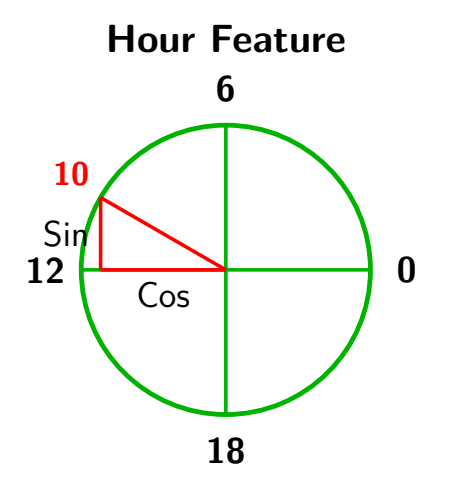
\includegraphics[keepaspectratio]{figure/fig_62fad448dfe46649.png}}
\caption{Slide 18 --- Ora del giorno rappresentata sulla circonferenza}
\end{figure}
% END F03-B0086

% BEGIN F03-B0087
Servono entrambe le coordinate per distinguere posizioni che una sola funzione confonderebbe: il seno, per esempio, vale zero sia a mezzanotte sia a mezzogiorno. Per l\textquotesingle ora 10, l\textquotesingle angolo è \(5\pi/6\) e la coppia \((\cos,\sin)\) è \((-\sqrt3/2,1/2)\), coerente con il punto nel secondo quadrante della figura.
% END F03-B0087

% BEGIN F03-B0088
La codifica periodica è appropriata per grandezze \textbf{effettivamente cicliche}. L\textquotesingle anno assoluto non riparte automaticamente da zero: non gli si impone un ciclo senza una ragione legata al problema. Inoltre coordinate limitate fra \(-1\) e 1 non garantiscono media empirica zero o una particolare varianza se i dati non coprono uniformemente il ciclo.
% END F03-B0088

% BEGIN F03-B0089
Il preprocessing costruisce le feature fornite al modello; non cambia la regola di ricorrenza. I richiami alla scala degli ingressi si collegano a \hyperref[fonte01]{Multilayer Perceptron} e, per il diverso caso della normalizzazione delle attivazioni interne, a \hyperref[fonte02]{reti convoluzionali}.
% END F03-B0089

% BEGIN F03-B0090
\section{Reti ricorrenti e forme dei problemi sequenziali (slide 19--21)}\label{f03-r230}
% END F03-B0090

% BEGIN F03-B0091
In una rete feedforward il calcolo procede dall\textquotesingle ingresso attraverso livelli intermedi fino all\textquotesingle uscita. Una RNN introduce una connessione di ritorno: \textbf{lo stato calcolato a un passo viene utilizzato nel passo successivo}. Il feedback riguarda qui la rappresentazione nascosta, non necessariamente la predizione finale.
% END F03-B0091

% BEGIN F03-B0092
La sequenza può comparire all\textquotesingle ingresso, all\textquotesingle uscita o in entrambi. I termini «one» e «many» contano gli elementi della sequenza, non il numero di componenti del singolo vettore.
% END F03-B0092

% BEGIN F03-B0093
\begin{longtable}[]{@{}
  >{\raggedright\arraybackslash}p{(\linewidth - 4\tabcolsep) * \real{0.3333}}
  >{\raggedright\arraybackslash}p{(\linewidth - 4\tabcolsep) * \real{0.3333}}
  >{\raggedright\arraybackslash}p{(\linewidth - 4\tabcolsep) * \real{0.3333}}@{}}
\toprule\noalign{}
\begin{minipage}[b]{\linewidth}\raggedright
Schema
\end{minipage} & \begin{minipage}[b]{\linewidth}\raggedright
Ingresso e uscita
\end{minipage} & \begin{minipage}[b]{\linewidth}\raggedright
Interpretazione
\end{minipage} \\
\midrule\noalign{}
\endhead
\bottomrule\noalign{}
\endlastfoot
\textbf{One-to-one} & Un elemento → un risultato & Situazione ordinaria non sequenziale \\
\textbf{One-to-many} & Un elemento → una sequenza & Un ingresso avvia più passi di uscita \\
\textbf{Many-to-one} & Una sequenza → un risultato & Sentiment o categoria di una frase \\
\textbf{Many-to-many con uscita successiva} & Sequenza osservata → sequenza prodotta & Traduzione o prosecuzione futura di una serie \\
\textbf{Many-to-many allineato} & Una uscita associata a ogni ingresso & Ingressi e uscite sono indicizzati lungo la stessa sequenza \\
\end{longtable}
% END F03-B0093

% BEGIN F03-B0094
\begin{figure}[H]
\centering
\pandocbounded{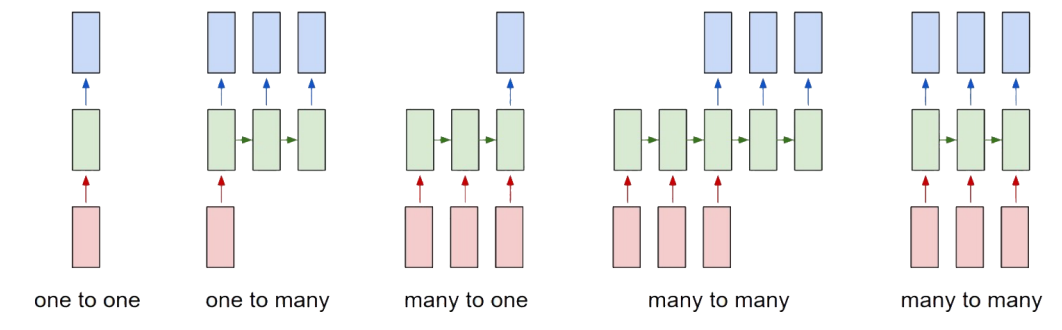
\includegraphics[keepaspectratio]{figure/fig_b9b03ce1d05693da.png}}
\caption{Slide 21 --- Schemi di ingresso e uscita delle reti sequenziali}
\end{figure}
% END F03-B0094

% BEGIN F03-B0095
Una frase può contenere molti token ma avere un solo target di classificazione; quel target può essere rappresentato da un vettore di score. Nel forecasting multipasso si osservano più valori e si prevedono più valori futuri. Nella traduzione, lunghezza dell\textquotesingle ingresso e lunghezza dell\textquotesingle uscita possono essere differenti. Anche domanda e risposta testuale illustrano il rapporto fra una sequenza in ingresso e una sequenza in uscita, senza che questo determini da solo l\textquotesingle architettura usata.
% END F03-B0095

% BEGIN F03-B0096
\section{Vanilla RNN: equazioni, dimensioni e significato (slide 22)}\label{f03-r248}
% END F03-B0096

% BEGIN F03-B0097
La forma più semplice, detta \textbf{vanilla RNN}, aggiorna lo stato mediante due contributi: l\textquotesingle osservazione corrente e lo stato precedente. Adottiamo vettori colonna e la notazione della slide 22:
% END F03-B0097

% BEGIN F03-B0098
\begin{center}
\begin{adjustbox}{max width=\linewidth}
$\displaystyle \boxed{\begin{aligned}
a_t&=Wh_{t-1}+Ux_t,\\
h_t&=\phi(a_t),\\
o_t&=Vh_t.
\end{aligned}}$
\end{adjustbox}
\end{center}
% END F03-B0098

% BEGIN F03-B0099
\begin{longtable}[]{@{}
  >{\raggedright\arraybackslash}p{(\linewidth - 4\tabcolsep) * \real{0.1444}}
  >{\raggedright\arraybackslash}p{(\linewidth - 4\tabcolsep) * \real{0.3889}}
  >{\raggedright\arraybackslash}p{(\linewidth - 4\tabcolsep) * \real{0.4667}}@{}}
\toprule\noalign{}
\begin{minipage}[b]{\linewidth}\raggedright
Simbolo
\end{minipage} & \begin{minipage}[b]{\linewidth}\raggedright
Forma
\end{minipage} & \begin{minipage}[b]{\linewidth}\raggedright
Ruolo
\end{minipage} \\
\midrule\noalign{}
\endhead
\bottomrule\noalign{}
\endlastfoot
\(x_t\) & \(d\times1\) & Osservazione al passo \(t\) \\
\(h_{t-1},h_t\) & \(m\times1\) & Stato nascosto precedente e corrente \\
\(a_t\) & \(m\times1\) & Pre-attivazione, prima della non linearità \\
\(U\) & \(m\times d\) & Proiezione ingresso → stato \\
\(W\) & \(m\times m\) & Trasformazione dello stato precedente \\
\(\phi\) & Applicata componente per componente & Attivazione, per esempio \(\tanh\) \\
\(V\) & \(r\times m\) & Proiezione stato → uscita \\
\(o_t\) & \(r\times1\) & Uscita o score del passo corrente \\
\end{longtable}
% END F03-B0099

% BEGIN F03-B0100
La dimensione \(m\) dello stato è una scelta architetturale, come la larghezza di un livello nascosto di un MLP. Anche una serie univariata può essere proiettata in uno stato di 256 componenti: \(d=1\) non impone \(m=1\).
% END F03-B0100

% BEGIN F03-B0101
\subsection{Come si costruisce un aggiornamento (slide 22)}\label{f03-r271}
% END F03-B0101

% BEGIN F03-B0102
La formula si legge verificando prima le dimensioni:
% END F03-B0102

% BEGIN F03-B0103
\begin{center}
\begin{adjustbox}{max width=\linewidth}
$\displaystyle 
\begin{aligned}
u_t&=Ux_t\in\mathbb R^m &&(m\times d)(d\times1)=m\times1,\\
v_t&=Wh_{t-1}\in\mathbb R^m &&(m\times m)(m\times1)=m\times1,\\
a_t&=u_t+v_t\in\mathbb R^m &&\text{somma di vettori della stessa forma},\\
h_t&=\phi(a_t)\in\mathbb R^m &&\text{attivazione componente per componente},\\
o_t&=Vh_t\in\mathbb R^r &&(r\times m)(m\times1)=r\times1.
\end{aligned}
$
\end{adjustbox}
\end{center}
% END F03-B0103

% BEGIN F03-B0104
Le trasformazioni portano ingresso e memoria nello stesso spazio; la somma li fonde; l\textquotesingle attivazione produce il nuovo stato. È lo schema del neurone di \hyperref[fonte01]{Multilayer Perceptron}, con un secondo ingresso che arriva dal passato.
% END F03-B0104

% BEGIN F03-B0105
Le slide omettono i bias per semplicità. Se presenti, si aggiungono un vettore \(b_h\in\mathbb R^m\) prima di \(\phi\) e un vettore \(b_o\in\mathbb R^r\) nell\textquotesingle uscita. L\textquotesingle omissione non implica che un\textquotesingle implementazione debba esserne priva.
% END F03-B0105

% BEGIN F03-B0106
\begin{figure}[H]
\centering
\pandocbounded{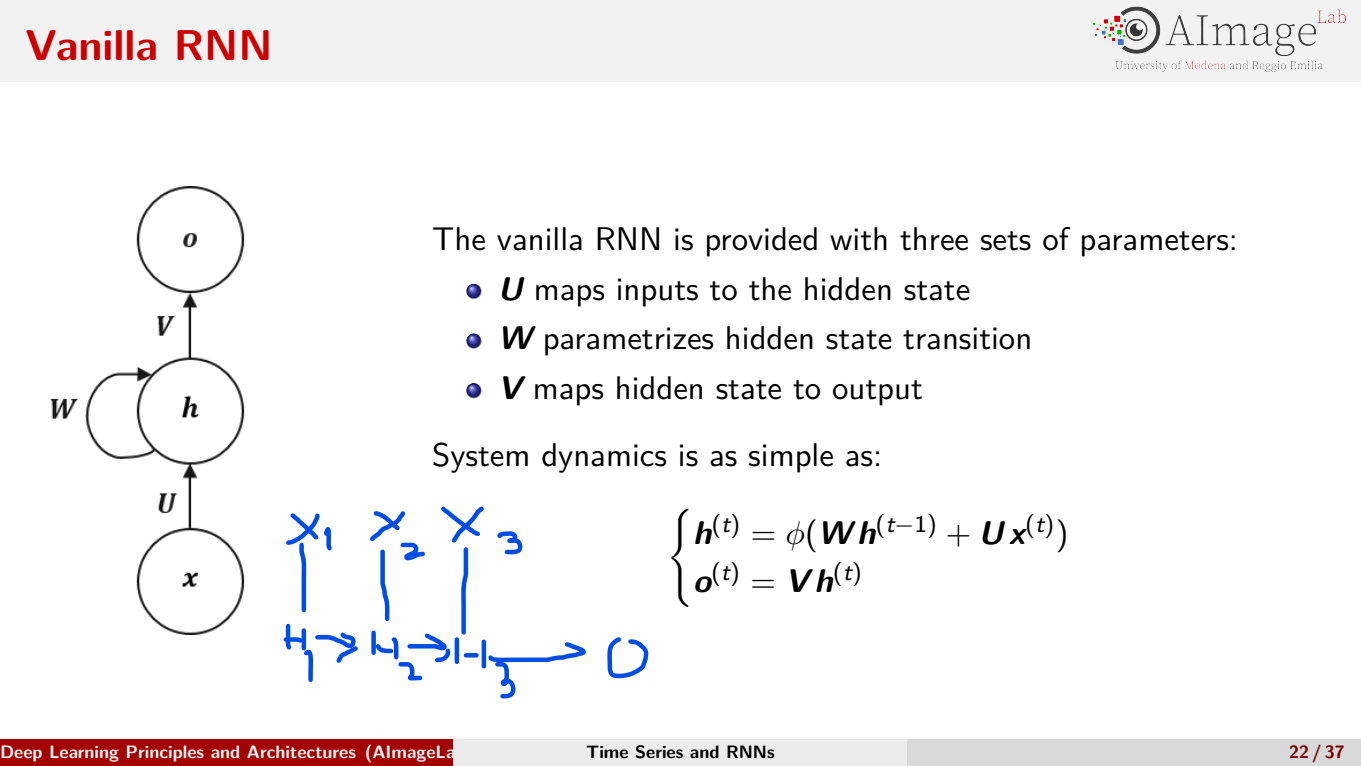
\includegraphics[keepaspectratio]{figure/fig_a3642bd8b36508e6.png}}
\caption{Slide 22 --- RNN con annotazione a mano dello srotolamento in tre passi}
\end{figure}
% END F03-B0106

% BEGIN F03-B0107
\subsection{Esempio numerico di un passo (slide 22)}\label{f03-r291}
% END F03-B0107

% BEGIN F03-B0108
Consideriamo due feature di ingresso, due unità nascoste e una uscita: \(d=m=2\), \(r=1\). Siano
% END F03-B0108

% BEGIN F03-B0109
\begin{center}
\begin{adjustbox}{max width=\linewidth}
$\displaystyle 
x_t=\begin{bmatrix}1\\2\end{bmatrix},\quad
h_{t-1}=\begin{bmatrix}0.5\\-0.5\end{bmatrix},\quad
U=\begin{bmatrix}1&0\\0&0.5\end{bmatrix},\quad
W=\begin{bmatrix}0.2&0\\0&0.2\end{bmatrix},\quad
V=\begin{bmatrix}1&-1\end{bmatrix}.
$
\end{adjustbox}
\end{center}
% END F03-B0109

% BEGIN F03-B0110
Applicando i passaggi precedenti:
% END F03-B0110

% BEGIN F03-B0111
\begin{center}
\begin{adjustbox}{max width=\linewidth}
$\displaystyle 
\begin{aligned}
Ux_t&=\begin{bmatrix}1\cdot1+0\cdot2\\0\cdot1+0.5\cdot2\end{bmatrix}
=\begin{bmatrix}1\\1\end{bmatrix},\\
Wh_{t-1}&=\begin{bmatrix}0.2\cdot0.5\\0.2\cdot(-0.5)\end{bmatrix}
=\begin{bmatrix}0.1\\-0.1\end{bmatrix},\\
a_t&=\begin{bmatrix}1.1\\0.9\end{bmatrix},\\
h_t&=\tanh(a_t)\approx\begin{bmatrix}0.800499\\0.716298\end{bmatrix},\\
o_t&=1\cdot0.800499-1\cdot0.716298\approx0.084201.
\end{aligned}
$
\end{adjustbox}
\end{center}
% END F03-B0111

% BEGIN F03-B0112
L\textquotesingle uscita è qui uno scalare generico. In classificazione può essere uno score su cui costruire la loss appropriata; in regressione può rappresentare la quantità da stimare. Una trasformazione lineare \(Vh_t\) non produce automaticamente probabilità.
% END F03-B0112

% BEGIN F03-B0113
\subsection{Lunghezza variabile e pesi condivisi (slide 22)}\label{f03-r319}
% END F03-B0113

% BEGIN F03-B0114
Per una sequenza di tre elementi il modello calcola:
% END F03-B0114

% BEGIN F03-B0115
\begin{center}
\begin{adjustbox}{max width=\linewidth}
$\displaystyle 
\begin{aligned}
h_1&=\phi(Wh_0+Ux_1),\\
h_2&=\phi(Wh_1+Ux_2),\\
h_3&=\phi(Wh_2+Ux_3).
\end{aligned}
$
\end{adjustbox}
\end{center}
% END F03-B0115

% BEGIN F03-B0116
Se arriva un quarto elemento si esegue un altro aggiornamento con \textbf{le stesse matrici}. Non si crea un nuovo insieme di pesi per ogni posizione. La ricorrenza cambia il numero delle iterazioni richieste, non la forma delle trasformazioni.
% END F03-B0116

% BEGIN F03-B0117
Senza bias e senza apprendere \(h_0\), il conteggio deriva dal numero di elementi delle tre matrici:
% END F03-B0117

% BEGIN F03-B0118
\begin{center}
\begin{adjustbox}{max width=\linewidth}
$\displaystyle 
\begin{aligned}
P_U&=md,\qquad P_W=m^2,\qquad P_V=rm,\\
\boxed{P_{\mathrm{RNN}}}&=\boxed{md+m^2+rm.}
\end{aligned}
$
\end{adjustbox}
\end{center}
% END F03-B0118

% BEGIN F03-B0119
Nell\textquotesingle esempio \(d=m=2,r=1\) sono \(4+4+2=10\) pesi, sia per una sequenza di 3 passi sia per una di 100. Due bias aggiungerebbero \(m+r=3\) parametri; uno stato iniziale apprendibile aggiungerebbe altri \(m=2\) valori. È il conteggio della parametrizzazione descritta, non una formula universale per qualsiasi implementazione multilivello.
% END F03-B0119

% BEGIN F03-B0120
La condivisione è temporale: nelle CNN lo stesso filtro viene riutilizzato in posizioni spaziali differenti; qui la stessa regola viene riutilizzata in istanti differenti. Più passi significano comunque più calcolo.
% END F03-B0120

% BEGIN F03-B0121
\section{Hidden state: un riassunto utile, non il modello appreso (slide 23)}\label{f03-r346}
% END F03-B0121

% BEGIN F03-B0122
Lo stato \(h_t\) può essere influenzato da tutti gli ingressi elaborati fino a \(t\), perché \(h_t\) dipende da \(h_{t-1}\), che dipende da \(h_{t-2}\), e così via. È un \textbf{riassunto della storia disponibile}, orientato al compito e generalmente con perdita di informazione. Una dimensione fissa \(m\) non equivale a memorizzare esplicitamente una lista che cresce con la sequenza.
% END F03-B0122

% BEGIN F03-B0123
Per una classificazione many-to-one si può usare lo stato finale \(h_T\) per ottenere la decisione. La RNN agisce da estrattore di feature temporali, come la parte convoluzionale estrae feature spaziali; sopra lo stato o la sua proiezione si può collegare un MLP.
% END F03-B0123

% BEGIN F03-B0124
\pandocbounded{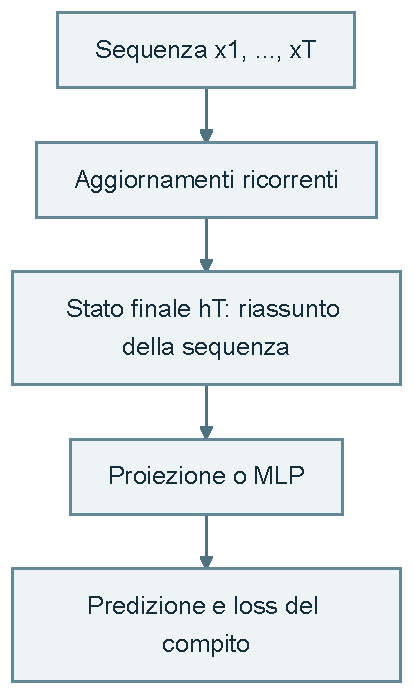
\includegraphics[keepaspectratio]{figure/diagramma_f03_02.pdf}}
% END F03-B0124

% BEGIN F03-B0125
Il riassunto non è necessariamente completo né sempre efficace: proprio l\textquotesingle apprendimento di informazioni lontane sarà il problema successivo. Il legame strutturale con il passato non garantisce che tutti gli elementi conservino la stessa influenza.
% END F03-B0125

% BEGIN F03-B0126
\subsection{Che cosa rimane dopo il training? (slide 23)}\label{f03-r362}
% END F03-B0126

% BEGIN F03-B0127
Le matrici \(U,W,V\) sono \textbf{parametri}, condivisi fra esempi. Lo stato \(h_t\) è una \textbf{attivazione}, calcolata per una specifica sequenza. Il risultato dell\textquotesingle apprendimento sono le matrici e gli eventuali altri parametri, non l\textquotesingle ultimo stato prodotto dall\textquotesingle ultimo esempio di training.
% END F03-B0127

% BEGIN F03-B0128
Su una nuova sequenza si inizializza lo stato e si ripete il forward. \(h_0\) può essere fissato, spesso a zero, oppure essere un parametro apprendibile. Per proseguire una stessa sequenza in inferenza è sufficiente mantenere lo stato corrente e aggiornarlo con la nuova osservazione; per esempi indipendenti non si trasferisce automaticamente la storia dell\textquotesingle esempio precedente.
% END F03-B0128

% BEGIN F03-B0129
In training, per calcolare i gradienti lungo la sequenza, servono invece gli intermedi del grafo o un modo di ricostruirli: dimensione fissa dello stato non significa memoria di addestramento indipendente da \(T\).
% END F03-B0129

% BEGIN F03-B0130
\subsection{Comporre CNN e RNN per un video (slide 23)}\label{f03-r370}
% END F03-B0130

% BEGIN F03-B0131
Un video è una sequenza di immagini. Una CNN può elaborare ciascun fotogramma e produrre un vettore di feature; la RNN può elaborare la successione di quei vettori. I due blocchi trattano rispettivamente struttura spaziale e ordine temporale.
% END F03-B0131

% BEGIN F03-B0132
\pandocbounded{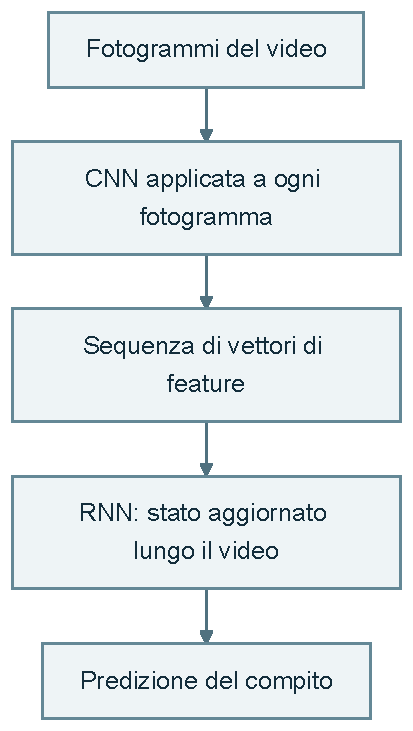
\includegraphics[keepaspectratio]{figure/diagramma_f03_03.pdf}}
% END F03-B0132

% BEGIN F03-B0133
È un esempio di composizione dei blocchi già studiati, senza introdurre una nuova regola di apprendimento.
% END F03-B0133

% BEGIN F03-B0134
\section{Unfolding: esplicitare il calcolo nel tempo (slide 24--26)}\label{f03-r384}
% END F03-B0134

% BEGIN F03-B0135
Il disegno con un arco che torna sullo stato è una rappresentazione compatta. Lo \textbf{srotolamento}, o \textbf{unfolding/unrolling}, esplicita un nodo per ogni aggiornamento. Ogni copia usa gli stessi parametri: non rappresenta una cella con pesi nuovi.
% END F03-B0135

% BEGIN F03-B0136
\begin{figure}[H]
\centering
\pandocbounded{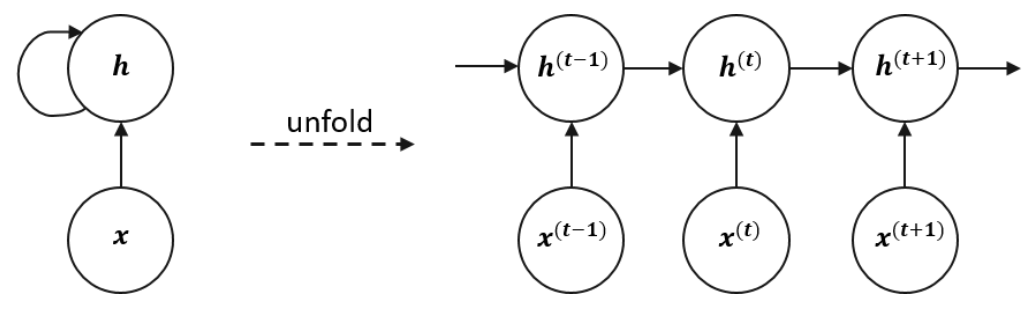
\includegraphics[keepaspectratio]{figure/fig_5cd686723b91f868.png}}
\caption{Slide 24 --- Grafo ricorrente e srotolamento}
\end{figure}
% END F03-B0136

% BEGIN F03-B0137
Per tre osservazioni e una sola uscita finale:
% END F03-B0137

% BEGIN F03-B0138
\pandocbounded{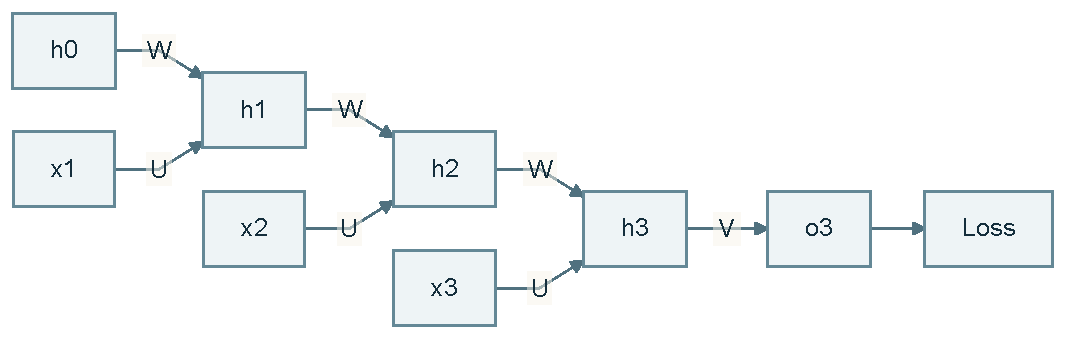
\includegraphics[keepaspectratio]{figure/diagramma_f03_04.pdf}}
% END F03-B0138

% BEGIN F03-B0139
\begin{figure}[H]
\centering
\pandocbounded{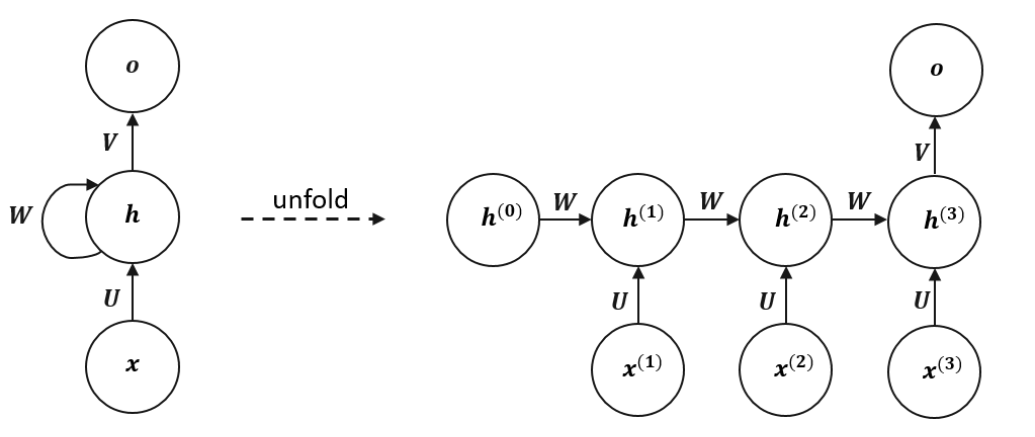
\includegraphics[keepaspectratio]{figure/fig_73242035e461b501.png}}
\caption{Slide 26 --- Esempio many-to-one con tre passi e stato iniziale}
\end{figure}
% END F03-B0139

% BEGIN F03-B0140
Una volta fissata una sequenza finita, il grafo srotolato è un \textbf{DAG}, un grafo diretto senza cicli: \(h_1\) dipende da \(h_0\), \(h_2\) da \(h_1\), e nessun nodo torna indietro modificando il valore di un nodo precedente nello stesso forward. L\textquotesingle arco di ritorno del disegno compatto indica il riutilizzo al passo successivo.
% END F03-B0140

% BEGIN F03-B0141
Si può quindi applicare la backpropagation ordinaria. Poiché il backward attraversa i passi temporali in ordine inverso, si parla di \textbf{Backpropagation Through Time}, abbreviata \textbf{BPTT}. La regola della catena è quella di \hyperref[fonte01]{Multilayer Perceptron}; qui le stesse matrici compaiono in più punti del grafo. Un sistema di differenziazione automatica può registrare questi passaggi e accumulare i gradienti corrispondenti.
% END F03-B0141

% BEGIN F03-B0142
\section{BPTT: sommare i contributi ai parametri condivisi (slide 27)}\label{f03-r410}
% END F03-B0142

% BEGIN F03-B0143
Consideriamo il caso mostrato: \(T=3\), un\textquotesingle uscita finale \(o_3=Vh_3\) e una loss differenziabile \(\mathcal L(y,o_3)\). Manteniamo vettori colonna, \(h_0\) inizialmente indipendente da \(U,W\) e bias omessi.
% END F03-B0143

% BEGIN F03-B0144
Definiamo:
% END F03-B0144

% BEGIN F03-B0145
\begin{center}
\begin{adjustbox}{max width=\linewidth}
$\displaystyle 
\boxed{g=\nabla_{o_3}\mathcal L\in\mathbb R^r,\qquad
D_t=\operatorname{diag}\bigl(\phi'(a_t)\bigr)\in\mathbb R^{m\times m}.}
$
\end{adjustbox}
\end{center}
% END F03-B0145

% BEGIN F03-B0146
La matrice diagonale \(D_t\) contiene una derivata di attivazione per ogni unità. Come già visto per l\textquotesingle MLP, la derivata della loss rispetto alla pre-attivazione combina il gradiente in arrivo con la derivata locale.
% END F03-B0146

% BEGIN F03-B0147
\subsection{Gradiente della proiezione finale V (slide 27)}\label{f03-r423}
% END F03-B0147

% BEGIN F03-B0148
Per ogni componente:
% END F03-B0148

% BEGIN F03-B0149
\begin{center}
\begin{adjustbox}{max width=\linewidth}
$\displaystyle 
\begin{aligned}
o_{3,j}&=\sum_{i=1}^{m}V_{ji}h_{3,i},\\
\frac{\partial o_{3,j}}{\partial V_{ji}}&=h_{3,i}
&&\text{derivata locale della combinazione lineare},\\
\frac{\partial\mathcal L}{\partial V_{ji}}&=g_jh_{3,i}
&&\text{regola della catena},\\
\boxed{\nabla_V\mathcal L}&=\boxed{g h_3^T\in\mathbb R^{r\times m}.}
\end{aligned}
$
\end{adjustbox}
\end{center}
% END F03-B0149

% BEGIN F03-B0150
È un \textbf{prodotto esterno}: un gradiente per ciascun peso. Nel grafo considerato \(V\) compare soltanto nella proiezione finale, quindi c\textquotesingle è un solo contributo locale. Il suo valore dipende comunque da \(h_3\), che riassume la sequenza: non significa che il passato sia irrilevante per \(V\).
% END F03-B0150

% BEGIN F03-B0151
\subsection{Gradiente attraverso gli stati (slide 27)}\label{f03-r440}
% END F03-B0151

% BEGIN F03-B0152
Poniamo \(\delta_t=\nabla_{a_t}\mathcal L\in\mathbb R^m\). Dall\textquotesingle uscita finale si torna prima allo stato e poi alla pre-attivazione:
% END F03-B0152

% BEGIN F03-B0153
\begin{center}
\begin{adjustbox}{max width=\linewidth}
$\displaystyle 
\begin{aligned}
\nabla_{h_3}\mathcal L&=V^Tg
&&\text{backward della trasformazione lineare},\\
\delta_3&=D_3V^Tg
&&\text{backward dell'attivazione},\\
\nabla_{h_2}\mathcal L&=W^T\delta_3
&&\text{dipendenza di }a_3\text{ da }h_2,\\
\delta_2&=D_2W^T\delta_3
&&\text{backward dell'attivazione al passo 2},\\
\delta_1&=D_1W^T\delta_2
&&\text{stessa regola al passo 1}.
\end{aligned}
$
\end{adjustbox}
\end{center}
% END F03-B0153

% BEGIN F03-B0154
In generale, quando la loss è soltanto sull\textquotesingle uscita finale:
% END F03-B0154

% BEGIN F03-B0155
\begin{center}
\begin{adjustbox}{max width=\linewidth}
$\displaystyle \boxed{\delta_T=D_TV^Tg,\qquad\delta_t=D_tW^T\delta_{t+1}\quad(t<T).}$
\end{adjustbox}
\end{center}
% END F03-B0155

% BEGIN F03-B0156
Tutti i prodotti restituiscono un vettore di \(m\) componenti. Se ci sono loss anche su uscite intermedie si aggiungono i contributi locali di quelle uscite: il caso della slide rimane quello con una sola loss finale.
% END F03-B0156

% BEGIN F03-B0157
\subsection{Perché compare una somma per W e U (slide 27)}\label{f03-r465}
% END F03-B0157

% BEGIN F03-B0158
La componente \(i\) della pre-attivazione è
% END F03-B0158

% BEGIN F03-B0159
\begin{center}
\begin{adjustbox}{max width=\linewidth}
$\displaystyle a_{t,i}=\sum_jW_{ij}h_{t-1,j}+\sum_\ell U_{i\ell}x_{t,\ell}.$
\end{adjustbox}
\end{center}
% END F03-B0159

% BEGIN F03-B0160
Trattando gli ingressi al singolo nodo come fissati, le derivate \textbf{locali} sono:
% END F03-B0160

% BEGIN F03-B0161
\begin{center}
\begin{adjustbox}{max width=\linewidth}
$\displaystyle 
\begin{aligned}
\left.\frac{\partial a_{t,i}}{\partial W_{ij}}\right|_{\mathrm{locale}}
&=h_{t-1,j},\\
\left.\frac{\partial a_{t,i}}{\partial U_{i\ell}}\right|_{\mathrm{locale}}
&=x_{t,\ell}.
\end{aligned}
$
\end{adjustbox}
\end{center}
% END F03-B0161

% BEGIN F03-B0162
Moltiplicando per \(\delta_{t,i}\) si ottiene il contributo di quella specifica occorrenza del parametro. Poiché il parametro è lo stesso in ogni passo, si sommano tutte le occorrenze:
% END F03-B0162

% BEGIN F03-B0163
\begin{center}
\begin{adjustbox}{max width=\linewidth}
$\displaystyle 
\boxed{\begin{aligned}
\nabla_W\mathcal L&=\sum_{t=1}^{T}\delta_t h_{t-1}^T\in\mathbb R^{m\times m},\\
\nabla_U\mathcal L&=\sum_{t=1}^{T}\delta_t x_t^T\in\mathbb R^{m\times d}.
\end{aligned}}
$
\end{adjustbox}
\end{center}
% END F03-B0163

% BEGIN F03-B0164
Per \(T=3\), per esempio:
% END F03-B0164

% BEGIN F03-B0165
\begin{center}
\begin{adjustbox}{max width=\linewidth}
$\displaystyle \nabla_W\mathcal L=\delta_1h_0^T+\delta_2h_1^T+\delta_3h_2^T.$
\end{adjustbox}
\end{center}
% END F03-B0165

% BEGIN F03-B0166
La \textbf{sovrapposizione degli effetti} consiste nel tenere conto di tutti i modi in cui un parametro condiviso influenza l\textquotesingle uscita. I prodotti dentro \(\delta_t\) trasportano l\textquotesingle effetto lungo un percorso; la somma combina le diverse occorrenze del peso. Somma fra contributi e prodotto lungo una catena hanno ruoli differenti.
% END F03-B0166

% BEGIN F03-B0167
\begin{quote}
\textbf{Errata slide 27 --- Derivate locali e stato iniziale}
\end{quote}
% END F03-B0167

% BEGIN F03-B0168
\begin{quote}
Le somme con \(\partial h^{(k)}/\partial W\) e \(\partial h^{(k)}/\partial U\) richiedono di intendere queste derivate come contributi \textbf{locali} dell\textquotesingle occorrenza del parametro al passo \(k\). Se fossero derivate totali, si conterebbero più volte percorsi già inclusi. Con aggiornamenti indicizzati da 1 a \(T\) e \(h_0\) indipendente dai pesi, le occorrenze sono \(k=1,\ldots,T\); il termine \(k=0\) della slide è nullo. Un \(h_0\) appreso ha il proprio gradiente, non un\textquotesingle ulteriore occorrenza di \(W\) o \(U\).
\end{quote}
% END F03-B0168

% BEGIN F03-B0169
Se \(h_0\) è apprendibile, il suo gradiente in questo esempio è \(W^T\delta_1\). Se c\textquotesingle è un bias nascosto condiviso, il contributo locale è \(\delta_t\) e il gradiente del bias è la loro somma. Sono le stesse regole di accumulo.
% END F03-B0169

% BEGIN F03-B0170
\subsection{Esempio numerico completo su tre passi (slide 26--27)}\label{f03-r502}
% END F03-B0170

% BEGIN F03-B0171
Per rendere trasparenti i conti, usiamo \textbf{solo in questo esempio} una ricorrenza scalare con attivazione identità: \(h_t=Wh_{t-1}+Ux_t\). Non è il caso non lineare con \(\tanh\) dell\textquotesingle esempio precedente; serve a isolare condivisione e regola della catena.
% END F03-B0171

% BEGIN F03-B0172
Siano \(h_0=0\), \(U=1\), \(W=0.5\), \(V=1\), ingressi \((x_1,x_2,x_3)=(1,2,0)\) e target \(y=1\). La loss è \(\mathcal L=\tfrac12(o_3-y)^2\), collegata alla MSE di \hyperref[fonte01]{Multilayer Perceptron}.
% END F03-B0172

% BEGIN F03-B0173
\begin{longtable}[]{@{}llr@{}}
\toprule\noalign{}
Passo & Calcolo dello stato & Risultato \\
\midrule\noalign{}
\endhead
\bottomrule\noalign{}
\endlastfoot
1 & \(0.5\cdot0+1\cdot1\) & \(h_1=1\) \\
2 & \(0.5\cdot1+1\cdot2\) & \(h_2=2.5\) \\
3 & \(0.5\cdot2.5+1\cdot0\) & \(h_3=1.25\) \\
\end{longtable}
% END F03-B0173

% BEGIN F03-B0174
Seguono \(o_3=1.25\) e \(\mathcal L=\tfrac12(0.25)^2=0.03125\). La derivata della loss è \(g=o_3-y=0.25\); con attivazione identità tutti i fattori \(D_t\) valgono 1:
% END F03-B0174

% BEGIN F03-B0175
\begin{center}
\begin{adjustbox}{max width=\linewidth}
$\displaystyle 
\begin{aligned}
\delta_3&=1\cdot1\cdot0.25=0.25,\\
\delta_2&=1\cdot0.5\cdot0.25=0.125,\\
\delta_1&=1\cdot0.5\cdot0.125=0.0625.
\end{aligned}
$
\end{adjustbox}
\end{center}
% END F03-B0175

% BEGIN F03-B0176
\begin{longtable}[]{@{}
  >{\raggedright\arraybackslash}p{(\linewidth - 4\tabcolsep) * \real{0.2727}}
  >{\raggedleft\arraybackslash}p{(\linewidth - 4\tabcolsep) * \real{0.3636}}
  >{\raggedleft\arraybackslash}p{(\linewidth - 4\tabcolsep) * \real{0.3636}}@{}}
\toprule\noalign{}
\begin{minipage}[b]{\linewidth}\raggedright
Passo
\end{minipage} & \begin{minipage}[b]{\linewidth}\raggedleft
Contributo a \(\partial\mathcal L/\partial W\)
\end{minipage} & \begin{minipage}[b]{\linewidth}\raggedleft
Contributo a \(\partial\mathcal L/\partial U\)
\end{minipage} \\
\midrule\noalign{}
\endhead
\bottomrule\noalign{}
\endlastfoot
1 & \(\delta_1h_0=0\) & \(\delta_1x_1=0.0625\) \\
2 & \(\delta_2h_1=0.125\) & \(\delta_2x_2=0.25\) \\
3 & \(\delta_3h_2=0.625\) & \(\delta_3x_3=0\) \\
\textbf{Somma} & \textbf{0.75} & \textbf{0.3125} \\
\end{longtable}
% END F03-B0176

% BEGIN F03-B0177
Per la proiezione finale, \(\partial\mathcal L/\partial V=g h_3=0.25\cdot1.25=0.3125\). Si può verificare anche sviluppando la ricorrenza:
% END F03-B0177

% BEGIN F03-B0178
\begin{center}
\begin{adjustbox}{max width=\linewidth}
$\displaystyle 
\begin{aligned}
h_1&=Ux_1,\\
h_2&=WUx_1+Ux_2,\\
h_3&=W^2Ux_1+WUx_2+Ux_3,\\
\frac{\partial h_3}{\partial W}&=2WUx_1+Ux_2=1+2=3,\\
\frac{\partial\mathcal L}{\partial W}&=gV\frac{\partial h_3}{\partial W}=0.25\cdot1\cdot3=0.75.
\end{aligned}
$
\end{adjustbox}
\end{center}
% END F03-B0178

% BEGIN F03-B0179
Il risultato coincide con la somma dei tre contributi. Il primo contributo locale a \(W\) è nullo perché \(h_0=0\), non perché il primo ingresso sia ignorato: \(x_1\) influenza anche gli stati successivi e il gradiente di \(U\).
% END F03-B0179

% BEGIN F03-B0180
Con un passo di gradient descent di ampiezza \(\eta=0.1\), tutti i gradienti vengono prima calcolati con gli stessi valori correnti, poi i parametri diventano \(W'=0.425\), \(U'=0.96875\) e \(V'=0.96875\). Non si modifica \(W\) a metà del backward per usarlo nella derivazione degli altri contributi.
% END F03-B0180

% BEGIN F03-B0181
\section{Dipendenze a lungo termine e instabilità del gradiente (slide 28--29)}\label{f03-r547}
% END F03-B0181

% BEGIN F03-B0182
Una dipendenza a lungo termine si presenta quando un\textquotesingle informazione ricevuta molto prima è utile alla predizione corrente. La RNN possiede un percorso che collega i due istanti, ma il gradiente deve attraversare tutti gli aggiornamenti intermedi per apprendere come conservare quell\textquotesingle informazione.
% END F03-B0182

% BEGIN F03-B0183
Definiamo la Jacobiana di una transizione:
% END F03-B0183

% BEGIN F03-B0184
\begin{center}
\begin{adjustbox}{max width=\linewidth}
$\displaystyle \boxed{J_t=\frac{\partial h_t}{\partial h_{t-1}}=D_tW\in\mathbb R^{m\times m}.}$
\end{adjustbox}
\end{center}
% END F03-B0184

% BEGIN F03-B0185
La formula si ricava da \(h_t=\phi(a_t)\) e \(a_t=Wh_{t-1}+Ux_t\): la derivata dell\textquotesingle attivazione è \(D_t\); la derivata della pre-attivazione rispetto allo stato precedente è \(W\). Per la regola della catena i due fattori si moltiplicano in quest\textquotesingle ordine.
% END F03-B0185

% BEGIN F03-B0186
\subsection{Il prodotto lungo il tempo (slide 28)}\label{f03-r557}
% END F03-B0186

% BEGIN F03-B0187
Con tre passi:
% END F03-B0187

% BEGIN F03-B0188
\begin{center}
\begin{adjustbox}{max width=\linewidth}
$\displaystyle 
\begin{aligned}
\frac{\partial h_3}{\partial h_1}
&=\frac{\partial h_3}{\partial h_2}\frac{\partial h_2}{\partial h_1}
&&\text{regola della catena},\\
&=J_3J_2
&&\text{definizione delle Jacobiane},\\
&=D_3WD_2W
&&\text{sostituzione delle derivate locali}.
\end{aligned}
$
\end{adjustbox}
\end{center}
% END F03-B0188

% BEGIN F03-B0189
In generale, per \(t>k\):
% END F03-B0189

% BEGIN F03-B0190
\begin{center}
\begin{adjustbox}{max width=\linewidth}
$\displaystyle \boxed{\frac{\partial h_t}{\partial h_k}=J_tJ_{t-1}\cdots J_{k+1}.}$
\end{adjustbox}
\end{center}
% END F03-B0190

% BEGIN F03-B0191
Il gradiente rispetto allo stato iniziale del tratto si ottiene moltiplicando il gradiente in arrivo per la trasposta di questo prodotto. Nel caso scalare sono semplicemente prodotti di derivate.
% END F03-B0191

% BEGIN F03-B0192
Se ogni fattore scalare vale \(0.5\), dieci transizioni danno \(0.5^{10}=0.0009765625\); venti danno circa \(9.54\cdot10^{-7}\). Un contributo partito con ampiezza 1 può quindi arrivare molto attenuato. Nell\textquotesingle esempio lineare della sezione precedente, \(J_t=W=0.5\) e \(\partial h_3/\partial h_1=0.25\).
% END F03-B0192

% BEGIN F03-B0193
Il \textbf{vanishing gradient} rende debole il segnale che dovrebbe insegnare alla rete a usare gli ingressi lontani. Non implica che ogni gradiente della rete sia nullo o che non rimanga alcuna informazione del passato: indica una difficoltà di apprendimento crescente lungo percorsi che contraggono ripetutamente il segnale.
% END F03-B0193

% BEGIN F03-B0194
\subsection{Derivata dell\textquotesingle attivazione e matrice ricorrente (slide 28)}\label{f03-r583}
% END F03-B0194

% BEGIN F03-B0195
Per \(\tanh\) e sigmoide, richiamando \hyperref[fonte01]{Multilayer Perceptron}:
% END F03-B0195

% BEGIN F03-B0196
\begin{center}
\begin{adjustbox}{max width=\linewidth}
$\displaystyle 
\boxed{\tanh'(a)=1-\tanh^2(a)\leq1,\qquad
\sigma'(a)=\sigma(a)(1-\sigma(a))\leq\tfrac14.}
$
\end{adjustbox}
\end{center}
% END F03-B0196

% BEGIN F03-B0197
Il limite della sigmoide si verifica completando il quadrato: posto \(s=\sigma(a)\in(0,1)\),
% END F03-B0197

% BEGIN F03-B0198
\begin{center}
\begin{adjustbox}{max width=\linewidth}
$\displaystyle 
\begin{aligned}
s(1-s)&=s-s^2,\\
&=\frac14-\left(s-\frac12\right)^2,\\
&\leq\frac14.
\end{aligned}
$
\end{adjustbox}
\end{center}
% END F03-B0198

% BEGIN F03-B0199
Per \(\tanh\), il quadrato è non negativo, quindi \(1-\tanh^2(a)\leq1\); in saturazione il quadrato è vicino a 1 e la derivata è piccola. Per esempio, \(\tanh'(0)=1\); \(\tanh'(2)\approx0.07065\). Per la sigmoide, \(\sigma'(0)=0.25\).
% END F03-B0199

% BEGIN F03-B0200
Questi sono i limiti delle \textbf{derivate delle attivazioni}, non della transizione completa. Per la norma spettrale, la proprietà \(\|AB\|_2\leq\|A\|_2\|B\|_2\) dà:
% END F03-B0200

% BEGIN F03-B0201
\begin{center}
\begin{adjustbox}{max width=\linewidth}
$\displaystyle 
\begin{aligned}
\|J_t\|_2&=\|D_tW\|_2\leq\|D_t\|_2\|W\|_2,\\
\left\|\frac{\partial h_t}{\partial h_k}\right\|_2
&\leq\prod_{j=k+1}^{t}\|J_j\|_2.
\end{aligned}
$
\end{adjustbox}
\end{center}
% END F03-B0201

% BEGIN F03-B0202
Se ogni fattore è al più \(c<1\), il prodotto è al più \(c^{t-k}\), che diminuisce geometricamente. Con \(c=0.5\) si ritrovano i numeri precedenti.
% END F03-B0202

% BEGIN F03-B0203
\begin{quote}
\textbf{Errata slide 28 --- Il limite non vale senza W}
\end{quote}
% END F03-B0203

% BEGIN F03-B0204
\begin{quote}
I limiti 1 per \(\tanh\) e \(1/4\) per sigmoide riguardano \(D_t\). La Jacobiana temporale è \(J_t=D_tW\) e dipende anche dai pesi. Per esempio, nel caso scalare con \(W=2\) e pre-attivazione zero, \(\tanh'(0)=1\) ma \(J_t=2\). Non si può dedurre dalla sola attivazione che ogni transizione abbia norma al più 1 o \(1/4\).
\end{quote}
% END F03-B0204

% BEGIN F03-B0205
\subsection{Exploding gradient e mitigazioni (slide 29)}\label{f03-r619}
% END F03-B0205

% BEGIN F03-B0206
L\textquotesingle effetto opposto si verifica quando i prodotti amplificano il gradiente. Dieci fattori scalari uguali a 2 danno 1024; venti danno 1 048 576. Aggiornamenti molto grandi possono rendere instabile l\textquotesingle ottimizzazione e produrre problemi numerici. Si parla di \textbf{exploding gradient}.
% END F03-B0206

% BEGIN F03-B0207
Un limite superiore grande non dimostra che ogni direzione venga amplificata: nei vettori contano anche i pesi, le attivazioni e la direzione del gradiente. Gli esempi scalari isolano il meccanismo.
% END F03-B0207

% BEGIN F03-B0208
Inizializzazione e scelta delle attivazioni influenzano questi prodotti. Il \textbf{gradient clipping} limita gradienti eccessivamente grandi; per chiarirne il significato, un clipping sulla norma ha la forma:
% END F03-B0208

% BEGIN F03-B0209
\begin{center}
\begin{adjustbox}{max width=\linewidth}
$\displaystyle \boxed{g_{\mathrm{clip}}=g\min\left(1,\frac{c}{\|g\|_2}\right),\qquad c>0,}$
\end{adjustbox}
\end{center}
% END F03-B0209

% BEGIN F03-B0210
con \(g_{\mathrm{clip}}=0\) se \(g=0\). Se \(\|g\|_2\leq c\), il minimo vale 1 e il gradiente non cambia. Se la norma supera \(c\), lo si moltiplica per \(c/\|g\|_2\), preservandone la direzione e portandone la norma a \(c\). Per \(g=(6,8)\) la norma è 10; con \(c=5\) il risultato è \((3,4)\), la cui norma è 5.
% END F03-B0210

% BEGIN F03-B0211
\begin{quote}
\textbf{Errata slide 29 --- Il clipping non recupera gradienti svaniti}
\end{quote}
% END F03-B0211

% BEGIN F03-B0212
\begin{quote}
Il clipping controlla soprattutto l\textquotesingle esplosione del gradiente. Non ricostruisce un contributo già diventato trascurabile. Inizializzazione, attivazioni e architettura intervengono sul flusso dei gradienti in modi differenti; non sono rimedi intercambiabili ai due problemi.
\end{quote}
% END F03-B0212

% BEGIN F03-B0213
Una RNN srotolata su molti passi crea una grande profondità temporale anche se contiene un solo livello ricorrente. Problemi analoghi possono comparire nelle reti feedforward profonde, come già discusso in \hyperref[fonte02]{reti convoluzionali} per le connessioni residue.
% END F03-B0213

% BEGIN F03-B0214
La condivisione dei pesi è una proprietà dell\textquotesingle architettura; la BPTT ne calcola correttamente le conseguenze, non la introduce. La difficoltà deriva dai lunghi prodotti di Jacobiane, non dalla sola presenza di parametri condivisi. Non basta inserire un logaritmo nel backward: il gradiente deve rimanere la derivata della funzione effettivamente calcolata. Per cambiarne i percorsi si interviene su modello e calcolo, non sostituendo arbitrariamente la regola della catena.
% END F03-B0214

% BEGIN F03-B0215
\section{Memoria selettiva e architetture con gate (slide 30)}\label{f03-r638}
% END F03-B0215

% BEGIN F03-B0216
La difficoltà delle dipendenze lontane motiva celle che possano imparare \textbf{quali informazioni conservare, quali aggiornare e quali esporre}. Le \textbf{Long Short-Term Memory}, o \textbf{LSTM}, introducono una memoria interna e gate apprendibili. Le \textbf{Gated Recurrent Unit}, o \textbf{GRU}, sono un\textquotesingle altra variante ricorrente, qui soltanto richiamata.
% END F03-B0216

% BEGIN F03-B0217
L\textquotesingle intuizione è accettare una memoria di dimensione fissata e imparare a gestirla. Non si può trattare lo stato come un archivio esplicito che contiene tutto il passato: conviene selezionare ciò che aiuta a ridurre la loss. Anche la vanilla RNN apprende una trasformazione selettiva degli ingressi; la differenza è che nella LSTM la selezione viene resa esplicita mediante gate e un percorso additivo della memoria.
% END F03-B0217

% BEGIN F03-B0218
Un \textbf{gate} si può immaginare come un interruttore graduabile. Un interruttore rigido lascia passare tutto o niente; un gate continuo può attenuare una componente in misura intermedia. I valori vicini a 1 lasciano passare quasi tutto, quelli vicini a 0 quasi nulla. Questa regolazione è appresa attraverso i pesi e la loss del compito, non impostata manualmente per ciascun ingresso.
% END F03-B0218

% BEGIN F03-B0219
Per le GRU basta qui ricordare il cenno conclusivo: impiegano \textbf{due gate}, comunemente detti aggiornamento e reset, e una struttura più compatta rispetto alla LSTM standard a parità di dimensioni. Non vengono sviluppate le equazioni GRU, né si deduce che due gate siano universalmente sufficienti per qualsiasi problema.
% END F03-B0219

% BEGIN F03-B0220
\section{LSTM: stato interno e quadro delle equazioni (slide 31)}\label{f03-r648}
% END F03-B0220

% BEGIN F03-B0221
La LSTM mantiene due vettori di dimensione \(m\):
% END F03-B0221

% BEGIN F03-B0222
\begin{itemize}
\tightlist
\item
  il \textbf{cell state} \(C_t\), la memoria interna;
\item
  lo \textbf{hidden state} \(h_t\), la rappresentazione esposta dalla cella.
\end{itemize}
% END F03-B0222

% BEGIN F03-B0223
Entrambi vengono aggiornati lungo la sequenza. Il simbolo \(o_t\) ora indica l\textquotesingle{}\textbf{output gate}: non è l\textquotesingle uscita \(o_t=Vh_t\) usata per la vanilla RNN. Per evitare ambiguità, una eventuale proiezione finale della LSTM sarà chiamata \(s_t\).
% END F03-B0223

% BEGIN F03-B0224
Le slide LSTM usano prodotti con vettori riga, mentre la slide 22 usava vettori colonna. Manteniamo qui la convenzione a colonne: la trasformazione \(x_tU_i\) della slide diventa \(U_ix_t\), con la matrice trasposta rispetto alla convenzione a righe. Non cambia l\textquotesingle operazione rappresentata.
% END F03-B0224

% BEGIN F03-B0225
Come nelle slide, i bias sono omessi. Il passo completo è:
% END F03-B0225

% BEGIN F03-B0226
\begin{center}
\begin{adjustbox}{max width=\linewidth}
$\displaystyle 
\boxed{\begin{aligned}
i_t&=\sigma(U_ix_t+W_ih_{t-1}),\\
f_t&=\sigma(U_fx_t+W_fh_{t-1}),\\
o_t&=\sigma(U_ox_t+W_oh_{t-1}),\\
\widetilde C_t&=\tanh(U_Cx_t+W_Ch_{t-1}),\\
C_t&=f_t\odot C_{t-1}+i_t\odot\widetilde C_t,\\
h_t&=o_t\odot\tanh(C_t).
\end{aligned}}
$
\end{adjustbox}
\end{center}
% END F03-B0226

% BEGIN F03-B0227
\begin{longtable}[]{@{}
  >{\raggedright\arraybackslash}p{(\linewidth - 4\tabcolsep) * \real{0.3333}}
  >{\raggedright\arraybackslash}p{(\linewidth - 4\tabcolsep) * \real{0.3333}}
  >{\raggedright\arraybackslash}p{(\linewidth - 4\tabcolsep) * \real{0.3333}}@{}}
\toprule\noalign{}
\begin{minipage}[b]{\linewidth}\raggedright
Quantità
\end{minipage} & \begin{minipage}[b]{\linewidth}\raggedright
Forma
\end{minipage} & \begin{minipage}[b]{\linewidth}\raggedright
Significato
\end{minipage} \\
\midrule\noalign{}
\endhead
\bottomrule\noalign{}
\endlastfoot
\(x_t\) & \(d\times1\) & Osservazione corrente \\
\(h_{t-1},h_t\) & \(m\times1\) & Stato nascosto precedente e corrente \\
\(C_{t-1},C_t\) & \(m\times1\) & Memoria precedente e corrente \\
\(i_t,f_t,o_t\) & \(m\times1\) & Gate di ingresso, mantenimento e uscita \\
\(\widetilde C_t\) & \(m\times1\) & Contenuto candidato da scrivere \\
\(U_i,U_f,U_o,U_C\) & \(m\times d\) & Pesi che elaborano l\textquotesingle ingresso \\
\(W_i,W_f,W_o,W_C\) & \(m\times m\) & Pesi che elaborano lo stato precedente \\
\(\odot\) & Operazione fra vettori della stessa forma & Prodotto elemento per elemento \\
\end{longtable}
% END F03-B0227

% BEGIN F03-B0228
\begin{figure}[H]
\centering
\pandocbounded{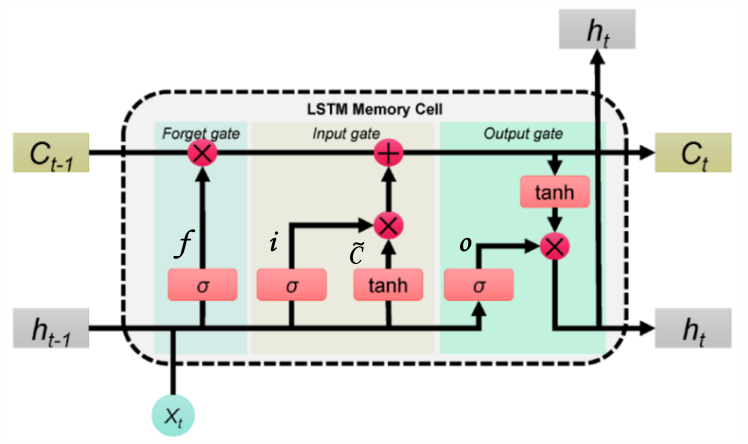
\includegraphics[keepaspectratio]{figure/fig_f0c5f113382b53d0.png}}
\caption{Slide 31 --- Schema della cella LSTM}
\end{figure}
% END F03-B0228

% BEGIN F03-B0229
Le equazioni non sono un risultato da dedurre dalla vanilla RNN: \textbf{definiscono la nuova architettura}. Per comprenderle si segue il flusso del calcolo: si costruiscono i gate e il candidato da \(x_t,h_{t-1}\); si aggiorna la memoria; si ricava lo stato nascosto. I passaggi seguenti esplicitano ogni operazione.
% END F03-B0229

% BEGIN F03-B0230
\section{Gate: interruttori continui apprendibili (slide 32)}\label{f03-r687}
% END F03-B0230

% BEGIN F03-B0231
Tutti i gate ricevono ingresso corrente e stato nascosto precedente, ma hanno \textbf{matrici proprie}. Per un gate generico \(g_t\):
% END F03-B0231

% BEGIN F03-B0232
\begin{center}
\begin{adjustbox}{max width=\linewidth}
$\displaystyle 
\begin{aligned}
z_{g,t}&=U_gx_t+W_gh_{t-1}\in\mathbb R^m
&&\text{combinazione delle due sorgenti},\\
g_{t,j}&=\sigma(z_{g,t,j})=\frac1{1+e^{-z_{g,t,j}}}\in(0,1)
&&\text{sigmoide per ciascuna componente}.
\end{aligned}
$
\end{adjustbox}
\end{center}
% END F03-B0232

% BEGIN F03-B0233
La sigmoide dà una quantità interpretabile come frazione da lasciare passare. Per esempio:
% END F03-B0233

% BEGIN F03-B0234
\begin{longtable}[]{@{}lrl@{}}
\toprule\noalign{}
Pre-attivazione & Gate risultante & Interpretazione \\
\midrule\noalign{}
\endhead
\bottomrule\noalign{}
\endlastfoot
\(0\) & \(0.5\) & Passaggio a metà \\
\(\ln3\) & \(1/(1+1/3)=0.75\) & Passaggio al 75\% \\
\(-\ln3\) & \(1/(1+3)=0.25\) & Passaggio al 25\% \\
\end{longtable}
% END F03-B0234

% BEGIN F03-B0235
Con pre-attivazioni finite, una sigmoide matematica è strettamente fra 0 e 1. I casi esatti 0 e 1 sono idealizzazioni utili per capire i meccanismi. La sigmoide è la scelta della cella descritta: il requisito concettuale è una selezione continua compatibile con l\textquotesingle apprendimento, non un teorema che impedisce ogni altro possibile gate.
% END F03-B0235

% BEGIN F03-B0236
\subsection{Prodotto di Hadamard (slide 31--32)}\label{f03-r710}
% END F03-B0236

% BEGIN F03-B0237
Il simbolo \(\odot\) è il \textbf{prodotto di Hadamard}:
% END F03-B0237

% BEGIN F03-B0238
\begin{center}
\begin{adjustbox}{max width=\linewidth}
$\displaystyle \boxed{(a\odot b)_j=a_jb_j.}$
\end{adjustbox}
\end{center}
% END F03-B0238

% BEGIN F03-B0239
Due vettori di \(m\) componenti producono un vettore di \(m\) componenti. Ogni posizione viene moltiplicata soltanto per la posizione corrispondente, senza sommare fra coordinate.
% END F03-B0239

% BEGIN F03-B0240
L\textquotesingle esempio dell\textquotesingle interruttore selettivo è:
% END F03-B0240

% BEGIN F03-B0241
\begin{center}
\begin{adjustbox}{max width=\linewidth}
$\displaystyle \begin{bmatrix}1\\2\\3\end{bmatrix}\odot\begin{bmatrix}0\\1\\0\end{bmatrix}
=\begin{bmatrix}1\cdot0\\2\cdot1\\3\cdot0\end{bmatrix}
=\begin{bmatrix}0\\2\\0\end{bmatrix}.$
\end{adjustbox}
\end{center}
% END F03-B0241

% BEGIN F03-B0242
Un gate può quindi conservare una componente e sopprimerne altre. È diverso sia da un prodotto scalare, che restituirebbe un solo numero, sia dalla trasformazione tramite una matrice che mescola componenti.
% END F03-B0242

% BEGIN F03-B0243
\subsection{I tre ruoli distinti (slide 32)}\label{f03-r726}
% END F03-B0243

% BEGIN F03-B0244
\begin{longtable}[]{@{}
  >{\raggedright\arraybackslash}p{(\linewidth - 4\tabcolsep) * \real{0.3333}}
  >{\raggedright\arraybackslash}p{(\linewidth - 4\tabcolsep) * \real{0.3333}}
  >{\raggedright\arraybackslash}p{(\linewidth - 4\tabcolsep) * \real{0.3333}}@{}}
\toprule\noalign{}
\begin{minipage}[b]{\linewidth}\raggedright
Gate
\end{minipage} & \begin{minipage}[b]{\linewidth}\raggedright
Dove interviene
\end{minipage} & \begin{minipage}[b]{\linewidth}\raggedright
Cosa controlla
\end{minipage} \\
\midrule\noalign{}
\endhead
\bottomrule\noalign{}
\endlastfoot
\textbf{Forget} \(f_t\) & \(f_t\odot C_{t-1}\) & Quanto della memoria precedente conservare \\
\textbf{Input} \(i_t\) & \(i_t\odot\widetilde C_t\) & Quanto del candidato scrivere nella memoria \\
\textbf{Output} \(o_t\) & \(o_t\odot\tanh(C_t)\) & Quanto dello stato trasformato esporre come \(h_t\) \\
\end{longtable}
% END F03-B0244

% BEGIN F03-B0245
Il nome \emph{forget gate} può trarre in inganno: un valore grande \textbf{conserva} il contenuto precedente; un valore piccolo lo attenua. La quantità scartata, lungo quel percorso, cresce quando \(f_t\) diminuisce. Il gate di ingresso filtra il candidato, che dipende anche da \(h_{t-1}\), non semplicemente i valori grezzi di \(x_t\).
% END F03-B0245

% BEGIN F03-B0246
\begin{quote}
\textbf{Errata slide 32 --- Interpretazione del forget gate}
\end{quote}
% END F03-B0246

% BEGIN F03-B0247
\begin{quote}
La descrizione in termini di memoria da «sovrascrivere» va letta attraverso l\textquotesingle equazione: il valore del forget gate è la frazione di memoria \textbf{conservata} sul percorso diretto. Un valore vicino a 1 non significa dimenticare tutto.
\end{quote}
% END F03-B0247

% BEGIN F03-B0248
I gate non sono tre RNN indipendenti con tre memorie nascoste separate: sono tre trasformazioni apprendibili che leggono lo stesso \(x_t\) e lo stesso \(h_{t-1}\) e operano in punti diversi della cella.
% END F03-B0248

% BEGIN F03-B0249
\section{Stato candidato: proporre un nuovo contenuto (slide 33)}\label{f03-r741}
% END F03-B0249

% BEGIN F03-B0250
Il candidato usa una combinazione di ingresso e stato precedente simile alla vanilla RNN:
% END F03-B0250

% BEGIN F03-B0251
\begin{center}
\begin{adjustbox}{max width=\linewidth}
$\displaystyle \boxed{\widetilde C_t=\tanh(U_Cx_t+W_Ch_{t-1})\in\mathbb R^m.}$
\end{adjustbox}
\end{center}
% END F03-B0251

% BEGIN F03-B0252
Prima si proiettano le due sorgenti nello stesso spazio, poi si sommano e si applica \(\tanh\). Le matrici sono proprie del candidato, distinte da quelle dei gate. Ogni componente del candidato è compresa fra \(-1\) e 1: può proporre un contributo positivo o negativo.
% END F03-B0252

% BEGIN F03-B0253
Per esempio, se una componente della pre-attivazione vale \(\ln3\), allora
% END F03-B0253

% BEGIN F03-B0254
\begin{center}
\begin{adjustbox}{max width=\linewidth}
$\displaystyle 
\begin{aligned}
\widetilde C_{t,j}
&=\tanh(\ln3)
=\frac{e^{\ln3}-e^{-\ln3}}{e^{\ln3}+e^{-\ln3}}\\
&=\frac{3-1/3}{3+1/3}=\frac{8/3}{10/3}=0.8.
\end{aligned}
$
\end{adjustbox}
\end{center}
% END F03-B0254

% BEGIN F03-B0255
È un contenuto \textbf{candidato}, non ancora la nuova memoria. Se il gate di ingresso corrispondente vale \(0.5\), la componente effettivamente scritta è \(0.5\cdot0.8=0.4\). Il modello separa così la proposta del contenuto dalla decisione su quanto scriverne.
% END F03-B0255

% BEGIN F03-B0256
\section{Aggiornare la memoria ed esporre lo stato (slide 34)}\label{f03-r762}
% END F03-B0256

% BEGIN F03-B0257
La memoria nuova combina due percorsi:
% END F03-B0257

% BEGIN F03-B0258
\begin{center}
\begin{adjustbox}{max width=\linewidth}
$\displaystyle \boxed{C_t=f_t\odot C_{t-1}+i_t\odot\widetilde C_t.}$
\end{adjustbox}
\end{center}
% END F03-B0258

% BEGIN F03-B0259
Per ciascuna componente:
% END F03-B0259

% BEGIN F03-B0260
\begin{center}
\begin{adjustbox}{max width=\linewidth}
$\displaystyle 
\begin{aligned}
p_{t,j}&=f_{t,j}C_{t-1,j} &&\text{parte conservata del passato},\\
n_{t,j}&=i_{t,j}\widetilde C_{t,j} &&\text{parte accettata del candidato},\\
C_{t,j}&=p_{t,j}+n_{t,j} &&\text{somma dei contributi}.
\end{aligned}
$
\end{adjustbox}
\end{center}
% END F03-B0260

% BEGIN F03-B0261
Non è obbligatoriamente una media pesata: \(f_{t,j}+i_{t,j}\) non deve essere 1. Le due selezioni sono apprese separatamente. Lo stato \(C_t\) non è perciò vincolato all\textquotesingle intervallo \([-1,1]\) del candidato.
% END F03-B0261

% BEGIN F03-B0262
Il secondo passaggio costruisce lo stato nascosto:
% END F03-B0262

% BEGIN F03-B0263
\begin{center}
\begin{adjustbox}{max width=\linewidth}
$\displaystyle \boxed{h_t=o_t\odot\tanh(C_t).}$
\end{adjustbox}
\end{center}
% END F03-B0263

% BEGIN F03-B0264
Prima si trasforma ogni componente della memoria con \(\tanh\), poi si applica il gate di uscita. La cella può conservare un contenuto in \(C_t\) e decidere di non esporlo pienamente in \(h_t\). Il risultato rimane un vettore di \(m\) componenti.
% END F03-B0264

% BEGIN F03-B0265
\pandocbounded{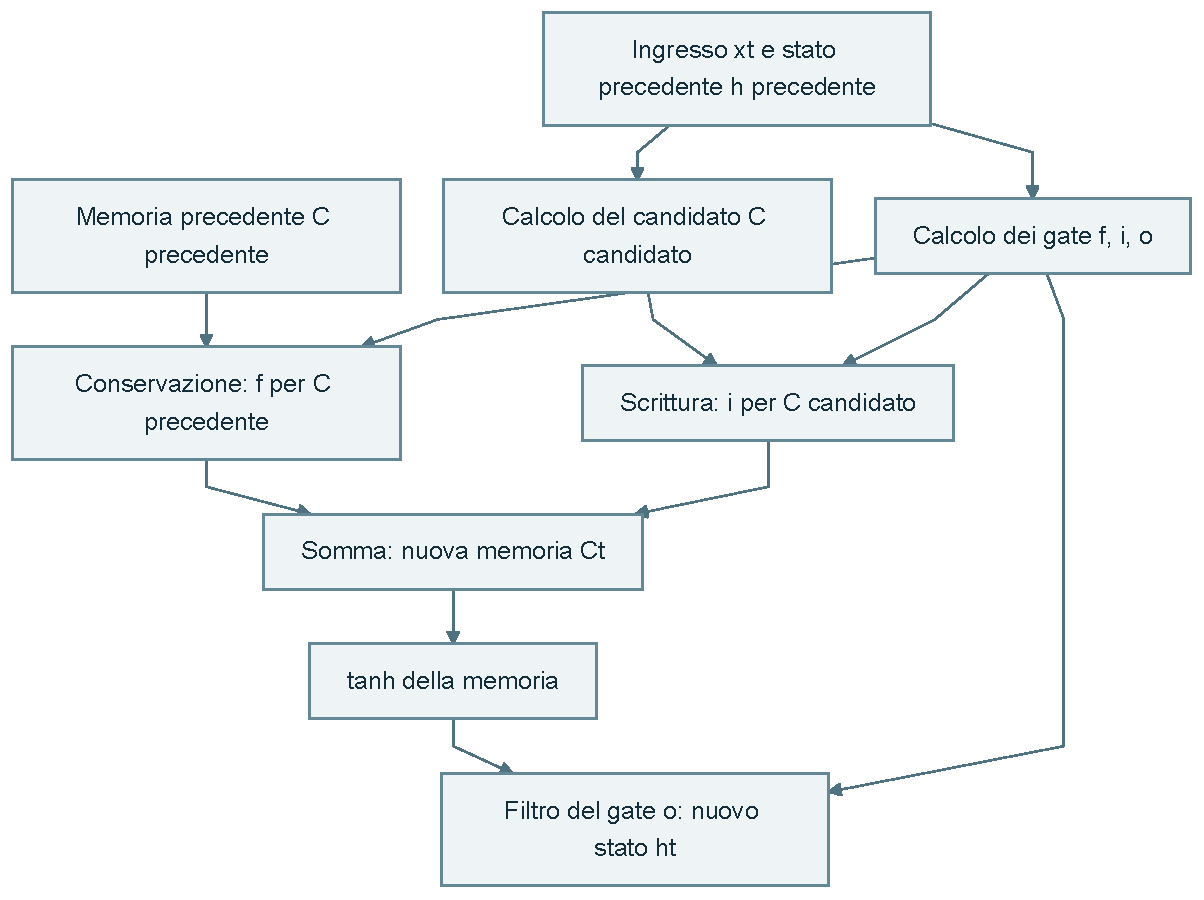
\includegraphics[keepaspectratio]{figure/diagramma_f03_05.pdf}}
% END F03-B0265

% BEGIN F03-B0266
\subsection{Che cosa accade quando un gate si chiude? (slide 34)}\label{f03-r801}
% END F03-B0266

% BEGIN F03-B0267
I casi limite rendono esplicito il significato delle formule:
% END F03-B0267

% BEGIN F03-B0268
\begin{longtable}[]{@{}
  >{\raggedright\arraybackslash}p{(\linewidth - 4\tabcolsep) * \real{0.3333}}
  >{\raggedright\arraybackslash}p{(\linewidth - 4\tabcolsep) * \real{0.3333}}
  >{\raggedright\arraybackslash}p{(\linewidth - 4\tabcolsep) * \real{0.3333}}@{}}
\toprule\noalign{}
\begin{minipage}[b]{\linewidth}\raggedright
Caso ideale, componente per componente
\end{minipage} & \begin{minipage}[b]{\linewidth}\raggedright
Nuova memoria
\end{minipage} & \begin{minipage}[b]{\linewidth}\raggedright
Significato
\end{minipage} \\
\midrule\noalign{}
\endhead
\bottomrule\noalign{}
\endlastfoot
\(f_t=1\), \(i_t=0\) & \(C_t=C_{t-1}\) & Conservare il passato senza nuova scrittura \\
\(f_t=0\), \(i_t=1\) & \(C_t=\widetilde C_t\) & Sostituire la memoria con il candidato \\
\(f_t=0\), \(i_t=0\) & \(C_t=0\) & Eliminare entrambi i contributi \\
\(i_t=0\), \(f_t=0.5\) & \(C_t=0.5C_{t-1}\) & Nessuna nuova scrittura, ma attenuazione del passato \\
\end{longtable}
% END F03-B0268

% BEGIN F03-B0269
Chiudere soltanto l\textquotesingle input gate non garantisce di conservare lo stato identico: rimane il fattore \(f_t\). Anche l\textquotesingle espressione «ignorare l\textquotesingle ingresso corrente» va intesa sul percorso di scrittura, perché \(x_t\) può continuare a influenzare gli altri gate.
% END F03-B0269

% BEGIN F03-B0270
Se l\textquotesingle output gate vale zero, \(h_t=0\) su quella componente, ma \(C_t\) può rimanere diverso da zero. Chiudere l\textquotesingle esposizione non equivale a cancellare la memoria.
% END F03-B0270

% BEGIN F03-B0271
\begin{quote}
\textbf{Errata slide 34 --- Indice della memoria precedente}
\end{quote}
% END F03-B0271

% BEGIN F03-B0272
\begin{quote}
Il testo descrittivo indica la memoria del passo precedente come \(C^{(t)}\): il simbolo corretto è \(C^{(t-1)}\). L\textquotesingle equazione dell\textquotesingle aggiornamento nella slide usa già l\textquotesingle indice corretto. Il forget gate pesa il contenuto precedente prima della somma con il candidato.
\end{quote}
% END F03-B0272

% BEGIN F03-B0273
\subsection{Esempio scalare completo della cella (slide 31--34)}\label{f03-r819}
% END F03-B0273

% BEGIN F03-B0274
Prendiamo \(d=m=1\), \(x_t=1\), \(h_{t-1}=0\) e \(C_{t-1}=2\). Poniamo tutti i pesi ricorrenti \(W_i,W_f,W_o,W_C\) a zero e scegliamo \(U_i=U_o=0\), \(U_f=U_C=\ln3\). I bias rimangono omessi.
% END F03-B0274

% BEGIN F03-B0275
\begin{longtable}[]{@{}llr@{}}
\toprule\noalign{}
Quantità & Calcolo & Valore \\
\midrule\noalign{}
\endhead
\bottomrule\noalign{}
\endlastfoot
Input gate & \(i_t=\sigma(0\cdot1+0\cdot0)\) & 0.5 \\
Forget gate & \(f_t=\sigma((\ln3)\cdot1+0\cdot0)\) & 0.75 \\
Output gate & \(o_t=\sigma(0\cdot1+0\cdot0)\) & 0.5 \\
Candidato & \(\widetilde C_t=\tanh((\ln3)\cdot1+0\cdot0)\) & 0.8 \\
Memoria conservata & \(f_tC_{t-1}=0.75\cdot2\) & 1.5 \\
Nuova scrittura & \(i_t\widetilde C_t=0.5\cdot0.8\) & 0.4 \\
Nuova memoria & \(C_t=1.5+0.4\) & 1.9 \\
Stato nascosto & \(h_t=0.5\tanh(1.9)\) & \(\approx0.478119\) \\
\end{longtable}
% END F03-B0275

% BEGIN F03-B0276
L\textquotesingle esempio verifica due punti: la memoria può superare 1 e la sua esposizione può essere attenuata dal gate di uscita. Il valore iniziale \(C_{t-1}=2\) è ammesso; con output gate precedente nullo si può anche avere \(h_{t-1}=0\) pur conservando memoria non nulla.
% END F03-B0276

% BEGIN F03-B0277
Con un\textquotesingle eventuale proiezione scalare \(s_t=2h_t\) si avrebbe \(s_t\approx0.956237\). Questa proiezione è esterna al meccanismo dei gate: il gate \(o_t=0.5\) non è la predizione finale.
% END F03-B0277

% BEGIN F03-B0278
\section{Perché separare cell state e hidden state (slide 35)}\label{f03-r838}
% END F03-B0278

% BEGIN F03-B0279
Il \textbf{cell state} offre un percorso di conservazione e aggiornamento additivo della memoria. Lo \textbf{hidden state} espone una versione trasformata e filtrata di tale memoria al resto della rete e al calcolo dei passi successivi.
% END F03-B0279

% BEGIN F03-B0280
L\textquotesingle interpretazione «memoria a lungo termine» per \(C_t\) e «a breve termine» per \(h_t\) descrive i loro ruoli, non due durate fissate. Non c\textquotesingle è un numero prestabilito di passi oltre il quale un contenuto debba scomparire: la conservazione dipende dai gate e dall\textquotesingle apprendimento.
% END F03-B0280

% BEGIN F03-B0281
\subsection{Percorso diretto della memoria e gradiente (slide 30--35)}\label{f03-r844}
% END F03-B0281

% BEGIN F03-B0282
Per chiarire il vantaggio rispetto alla vanilla RNN, consideriamo il percorso diretto da \(C_{t-1}\) a \(C_t\), mantenendo fissi gate e candidato. Per la componente \(j\):
% END F03-B0282

% BEGIN F03-B0283
\begin{center}
\begin{adjustbox}{max width=\linewidth}
$\displaystyle 
\begin{aligned}
C_{t,j}&=f_{t,j}C_{t-1,j}+i_{t,j}\widetilde C_{t,j},\\
\left.\frac{\partial C_{t,j}}{\partial C_{t-1,j}}\right|_{\mathrm{diretto}}
&=f_{t,j}
&&\text{derivata del termine lineare nella memoria},\\
\left.\frac{\partial C_t}{\partial C_{t-1}}\right|_{\mathrm{diretto}}
&=\operatorname{diag}(f_t)
&&\text{aggiornamento separato per componente}.
\end{aligned}
$
\end{adjustbox}
\end{center}
% END F03-B0283

% BEGIN F03-B0284
Se un gate di mantenimento è vicino a 1 per più passi, questo percorso può trasportare la memoria e il relativo gradiente senza imporre ogni volta una nuova moltiplicazione per \(W\) e una nuova derivata di \(\tanh\) come nella catena della vanilla RNN. Per esempio, dieci fattori \(0.99\) danno \(0.99^{10}\approx0.9044\), contro \(0.5^{10}\approx0.0009766\).
% END F03-B0284

% BEGIN F03-B0285
Si tratta del \textbf{contributo diretto}, non della derivata totale della cella: gate e candidato dipendono anche da \(h_{t-1}\) e quindi introducono altri percorsi. Le LSTM mitigano la difficoltà delle dipendenze lontane; non garantiscono memoria infinita né assenza di vanishing o exploding gradient in ogni condizione.
% END F03-B0285

% BEGIN F03-B0286
La conservazione rimane orientata alla loss: i gate non hanno un criterio esterno che stabilisca cosa sia interessante. La BPTT aggiorna le loro matrici affinché la selezione aiuti la predizione del target. L\textquotesingle intuizione di un interruttore è utile, ma la selezione è continua e differenziabile, non una decisione simbolica separata.
% END F03-B0286

% BEGIN F03-B0287
\subsection{Confine della trattazione e collegamenti (slide 35; riferimenti 36--37)}\label{f03-r866}
% END F03-B0287

% BEGIN F03-B0288
La trattazione delle slide termina con i due stati della LSTM. Il cenno alle GRU resta limitato alla variante con due gate e alla maggiore compattezza; non sono state sviluppate le relative equazioni. La bibliografia della slide 36 richiama i lavori su LSTM, GRU e difficoltà dell\textquotesingle addestramento ricorrente; la slide 37 contiene ringraziamenti.
% END F03-B0288

% BEGIN F03-B0289
I Transformer sono soltanto anticipati come successivo argomento: possono evitare la specifica catena di transizioni ricorrenti lungo il tempo, ma non è corretto trasformare questo richiamo nella garanzia che eliminino ogni difficoltà dei gradienti. La loro architettura non viene aggiunta a questa nota. Il laboratorio RNN è annunciato, senza sviluppare qui codice PyTorch non presente nelle fonti della lezione.
% END F03-B0289

% BEGIN F03-B0290
I collegamenti utili per il ripasso sono \hyperref[fonte01]{Multilayer Perceptron} per neurone, attivazioni, loss e regola della catena; \hyperref[fonte02]{reti convoluzionali} per condivisione dei pesi, composizione dei blocchi e connessioni residue; manuale introduttivo di Machine Learning (documento separato) per regressione e ottimizzazione.
% END F03-B0290

% BEGIN F03-B0291
\section{Riepilogo operativo (slide 4--35)}\label{f03-r874}
% END F03-B0291

% BEGIN F03-B0292
\begin{longtable}[]{@{}
  >{\raggedright\arraybackslash}p{(\linewidth - 4\tabcolsep) * \real{0.3333}}
  >{\raggedright\arraybackslash}p{(\linewidth - 4\tabcolsep) * \real{0.3333}}
  >{\raggedright\arraybackslash}p{(\linewidth - 4\tabcolsep) * \real{0.3333}}@{}}
\toprule\noalign{}
\begin{minipage}[b]{\linewidth}\raggedright
Concetto
\end{minipage} & \begin{minipage}[b]{\linewidth}\raggedright
Formula o forma
\end{minipage} & \begin{minipage}[b]{\linewidth}\raggedright
Interpretazione e condizioni
\end{minipage} \\
\midrule\noalign{}
\endhead
\bottomrule\noalign{}
\endlastfoot
Sequenza & \(X\in\mathbb R^{T\times d}\) & \(T\) passi, \(d\) feature per passo; \(T\) può variare \\
Codifica periodica & \((\cos(2\pi k/P),\sin(2\pi k/P))\) & Preserva la vicinanza a cavallo del ciclo \\
AR(\(p\)) & \(x_t=\sum_{i=1}^p\phi_ix_{t-i}+\xi_t\) & Dipendenza lineare dai ritardi più innovazione \\
Stato RNN & \(h_t=\phi(Wh_{t-1}+Ux_t)\) & Ingresso corrente e storia compressa \\
Uscita RNN & \(o_t=Vh_t\) & Score o quantità di uscita, non automaticamente probabilità \\
Dimensioni dei pesi & \(U:m\times d\), \(W:m\times m\), \(V:r\times m\) & Convenzione a vettori colonna \\
Pesi RNN & \(md+m^2+rm\) & Senza bias o stato iniziale appreso; indipendenti da \(T\) \\
Jacobiana temporale & \(J_t=D_tW\) & Include derivata dell\textquotesingle attivazione e pesi ricorrenti \\
Dipendenza lontana & \(\partial h_t/\partial h_k=J_t\cdots J_{k+1}\) & Prodotto delle transizioni intermedie \\
BPTT finale & \(\delta_T=D_TV^Tg\), \(\delta_t=D_tW^T\delta_{t+1}\) & Una sola loss finale; \(g=\nabla_{o_T}\mathcal L\) \\
Gradiente di \(V\) & \(g h_T^T\) & Prodotto esterno alla proiezione finale \\
Gradienti condivisi & \(\nabla_W\mathcal L=\sum_t\delta_th_{t-1}^T\), \(\nabla_U\mathcal L=\sum_t\delta_tx_t^T\) & Si sommano le occorrenze dello stesso parametro \\
Gate LSTM & \(g_t=\sigma(U_gx_t+W_gh_{t-1})\) & Un valore fra 0 e 1 per componente; \(g=i,f,o\) \\
Candidato LSTM & \(\widetilde C_t=\tanh(U_Cx_t+W_Ch_{t-1})\) & Proposta di contenuto da filtrare con \(i_t\) \\
Memoria LSTM & \(C_t=f_t\odot C_{t-1}+i_t\odot\widetilde C_t\) & Conservazione più scrittura; non necessariamente media \\
Hidden state LSTM & \(h_t=o_t\odot\tanh(C_t)\) & Esposizione filtrata della memoria \\
\end{longtable}
% END F03-B0292

% BEGIN F03-B0293
\begin{quote}
\textbf{Da saper spiegare}
\end{quote}
% END F03-B0293

% BEGIN F03-B0294
\begin{quote}
Una RNN riusa le stesse matrici per aggiornare uno stato di dimensione fissata, quindi può elaborare sequenze di lunghezza variabile. La BPTT applica la regola della catena al grafo srotolato e somma i contributi ai pesi condivisi. I lunghi prodotti di Jacobiane possono attenuare o amplificare il gradiente. La LSTM introduce una memoria con aggiornamento additivo e tre gate apprendibili: conservare il passato, scrivere il candidato ed esporre lo stato sono operazioni distinte.
\end{quote}
% END F03-B0294

% BEGIN F03-B0295
\section{Errata e precisazioni da conservare nel ripasso (slide 4--35)}\label{f03-r898}
% END F03-B0295

% BEGIN F03-B0296
\begin{longtable}[]{@{}
  >{\raggedright\arraybackslash}p{(\linewidth - 2\tabcolsep) * \real{0.5000}}
  >{\raggedright\arraybackslash}p{(\linewidth - 2\tabcolsep) * \real{0.5000}}@{}}
\toprule\noalign{}
\begin{minipage}[b]{\linewidth}\raggedright
Riferimento
\end{minipage} & \begin{minipage}[b]{\linewidth}\raggedright
Correzione o precisazione
\end{minipage} \\
\midrule\noalign{}
\endhead
\bottomrule\noalign{}
\endlastfoot
Slide 4 & Discreto non significa finito; il campione osservato è finito, il processo può proseguire. \\
Slide 6--8 & Stagionalità e ciclo non richiedono la stessa periodicità rigida; residuo non equivale automaticamente a rumore bianco. Media e varianza non esauriscono la stazionarietà. \\
Slide 10 & Un processo stocastico noto può mantenere innovazioni imprevedibili: conoscere il DGP non dà sempre il valore futuro esatto. \\
Slide 11 & Una fascia nel grafico non prova copertura al 90\% o gaussianità; l\textquotesingle incertezza è rappresentata, non derivata qui. \\
Slide 12 & Per prevedere \(x_t\) con \(q\) ritardi usare \(x_{t-1},\ldots,x_{t-q}\); lo schema dei disturbi non esplicita l\textquotesingle innovazione corrente. \\
Slide 13--14 & Rumore bianco non implica gaussianità; nel MA \(\mu\) è la media del processo, stimabile mediante la media empirica. \\
Slide 18 & Usare codifiche cicliche per periodi effettivi; l\textquotesingle anno assoluto non è automaticamente ciclico. Media empirica zero non è garantita dalla sola coppia seno-coseno. \\
Slide 22--23 & \(U,W,V\) sono parametri; \(h_t\) è un\textquotesingle attivazione della sequenza. Lunghezza variabile non significa numero di feature variabile. \\
Slide 24--27 & Lo srotolamento riusa i pesi; la BPTT non crea la condivisione. La profondità temporale cresce con i passi. \\
Slide 27 & Le derivate nella somma devono essere locali; per \(h_0\) indipendente dai pesi il termine \(k=0\) è nullo. Il gradiente di \(V\) usa lo stato finale, che dipende dalla storia. \\
Slide 28 & La Jacobiana della transizione è \(D_tW\), non la sola derivata dell\textquotesingle attivazione. \\
Slide 29 & Il clipping limita gradienti grandi, senza ricostruire contributi già svaniti. \\
Slide 30--32 & I gate sono continui, non bit rigidi; il forget gate alto conserva, basso attenua. La LSTM non è l\textquotesingle unico modello con memoria di dimensione fissata. \\
Slide 31 & Notazione LSTM a righe convertita coerentemente a colonne; l\textquotesingle output gate \(o_t\) è distinto dallo score della RNN. \\
Slide 34 & La memoria precedente è \(C_{t-1}\). Con \(i_t=0\) rimane \(f_t\odot C_{t-1}\): identità solo se anche \(f_t=1\) nelle componenti considerate. \\
Slide 35 & LSTM e GRU mitigano il problema delle dipendenze lontane; non garantiscono conservazione illimitata o stabilità assoluta. \\
\end{longtable}
% END F03-B0296

% BEGIN F03-B0297
Le forme trascritte come «Adamart/Adamard», «EFO» e «bad propagation» sono ricondotte rispettivamente a \textbf{Hadamard}, ai gate \textbf{\(i,f,o\)} e alla \textbf{backpropagation}, coerentemente con formule e contesto. I frammenti non intelligibili della domanda sul confronto con altri regressori non consentono di ricostruire un metodo preciso e non sono trasformati in contenuti aggiuntivi.
% END F03-B0297


% BEGIN F04-B0001
\chapter{TCN - Temporal Convolutional Networks}\label{argomento-tcn}
% END F04-B0001

% BEGIN F04-B0002
\begin{indiceargomento}
\item \hyperref[f04-r35]{Modelli per sequenze: l\textquotesingle ordine è informazione (slide 3--4)}
\item \hyperref[f04-r45]{Dalla convoluzione 2D alla convoluzione 1D (slide 5--8)}
\item \hyperref[f04-r135]{Dilatazione: ampliare la regione osservata senza nuovi pesi (slide 9)}
\item \hyperref[f04-r165]{Causalità: non leggere un futuro indisponibile (slide 10)}
\item \hyperref[f04-r190]{Temporal Convolutional Network: gerarchia e blocchi residui (slide 11)}
\item \hyperref[f04-r228]{Caso di studio finanziario: dati, baseline e risultati (slide 12--13)}
\item \hyperref[f04-r251]{TCN e RNN: memoria, parallelismo e spiegazioni (slide 14)}
\end{indiceargomento}
% END F04-B0002

% BEGIN F04-B0003
Le sequenze possono essere elaborate senza una ricorrenza sullo stato nascosto. Una prima possibilità consiste nello spostare un filtro convoluzionale lungo il tempo; una seconda nel costruire relazioni fra elementi mediante \textbf{attention}, con coefficienti che dipendono dall\textquotesingle ingresso corrente. Le \textbf{Temporal Convolutional Networks} (TCN) e i \textbf{Transformer} realizzano queste due idee.
% END F04-B0003

% BEGIN F04-B0004
\pandocbounded{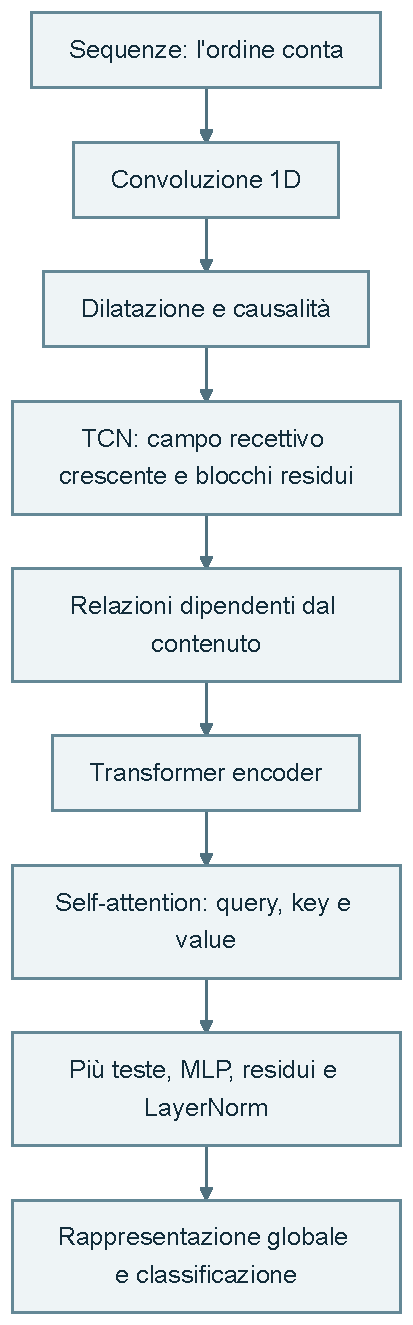
\includegraphics[keepaspectratio]{figure/diagramma_f04_01.pdf}}
% END F04-B0004

% BEGIN F04-B0005
\section{Modelli per sequenze: l\textquotesingle ordine è informazione (slide 3--4)}\label{f04-r35}
% END F04-B0005

% BEGIN F04-B0006
Un modello sequenziale riceve una successione di elementi e produce un risultato oppure un\textquotesingle altra successione. Gli elementi possono essere misure numeriche, parole, lettere, segnali audio o rappresentazioni di immagini. Una traduzione può trasformare «Je suis étudiant» in «I am a student»: il numero di elementi in ingresso e in uscita può essere diverso.
% END F04-B0006

% BEGIN F04-B0007
L\textquotesingle ordine modifica il significato. Nel testo, cambiare la posizione di soggetto e oggetto può cambiare chi compie un\textquotesingle azione; nelle serie temporali, scambiare due misure cambia l\textquotesingle evoluzione osservata. Traduzione, forecasting, descrizione di video, generazione audio e riassunto di testi sono esempi di compiti sequenziali.
% END F04-B0007

% BEGIN F04-B0008
Una sequenza di \(T\) osservazioni con \(C\) feature per osservazione si può disporre in una matrice \(X\in\mathbb R^{T\times C}\), con un\textquotesingle osservazione per riga. Qui l\textquotesingle indice temporale può anche indicare semplicemente una posizione nel testo. La distinzione fra lunghezza e numero di feature è quella introdotta in \hyperref[fonte03]{reti ricorrenti}.
% END F04-B0008

% BEGIN F04-B0009
Una RNN elabora gli ingressi successivamente e li riassume nello stato. Le alternative qui considerate mantengono invece una sequenza di rappresentazioni intermedie: le convoluzioni la trasformano con finestre locali; l\textquotesingle attention mette in relazione elementi in base al loro contenuto.
% END F04-B0009

% BEGIN F04-B0010
\section{Dalla convoluzione 2D alla convoluzione 1D (slide 5--8)}\label{f04-r45}
% END F04-B0010

% BEGIN F04-B0011
Una convoluzione sulle immagini sposta il kernel lungo altezza e larghezza. Per una sequenza basta un solo asse di scorrimento: il tempo o la posizione. Le feature di ogni osservazione svolgono il ruolo dei canali dell\textquotesingle immagine.
% END F04-B0011

% BEGIN F04-B0012
\textbf{Una convoluzione 1D ha un solo asse di scorrimento, non necessariamente un solo peso per posizione.} Un filtro su una finestra di \(k\) elementi, ciascuno con \(C_{\mathrm{in}}\) feature, contiene \(kC_{\mathrm{in}}\) pesi, più un eventuale bias. Il kernel copre tutti i canali e scorre lungo la sequenza, come descritto per i canali in \hyperref[fonte02]{reti convoluzionali}.
% END F04-B0012

% BEGIN F04-B0013
\begin{figure}[H]
\centering
\pandocbounded{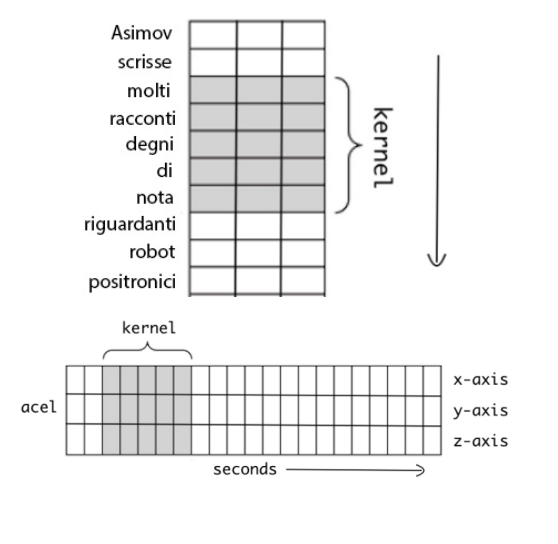
\includegraphics[keepaspectratio]{figure/fig_7430da53841d851d.png}}
\caption{Slide 7 --- Finestre su testo e segnale multivariato}
\end{figure}
% END F04-B0013

% BEGIN F04-B0014
\subsection{Operazione scalare e multicanale (slide 7)}\label{f04-r53}
% END F04-B0014

% BEGIN F04-B0015
La convoluzione discreta scalare riportata nelle slide è
% END F04-B0015

% BEGIN F04-B0016
\begin{center}
\begin{adjustbox}{max width=\linewidth}
$\displaystyle \boxed{y_t=(x*\omega)(t)=\sum_{i=0}^{k-1}x*(t-i)\omega_i.}$
\end{adjustbox}
\end{center}
% END F04-B0016

% BEGIN F04-B0017
\(x_t,y_t,\omega_i\) sono scalari; \(k\) è il numero di coefficienti del filtro. Si prende una finestra di valori, si moltiplica ogni valore per il peso associato e si sommano i risultati. Per \(k=3\):
% END F04-B0017

% BEGIN F04-B0018
\begin{center}
\begin{adjustbox}{max width=\linewidth}
$\displaystyle 
\begin{aligned}
y_t&=x_t\omega_0+x_{t-1}\omega_1+x_{t-2}\omega_2
&&\text{sviluppo della sommatoria}.
\end{aligned}
$
\end{adjustbox}
\end{center}
% END F04-B0018

% BEGIN F04-B0019
Con valori correnti e passati \((3,2,1)\) e pesi \((1,0,-1)\) si ottiene \(3\cdot1+2\cdot0+1\cdot(-1)=2\). La formula usa pesi ordinati per ritardo; all\textquotesingle inizio della serie occorre precisare come trattare gli indici mancanti, per esempio mediante padding.
% END F04-B0019

% BEGIN F04-B0020
Per l\textquotesingle esempio a finestre delle slide è più comoda la notazione di \textbf{correlazione incrociata} senza ribaltamento del kernel, come già chiarito in \hyperref[fonte02]{reti convoluzionali}. Per una finestra che parte in \(t\), con stride 1:
% END F04-B0020

% BEGIN F04-B0021
\begin{center}
\begin{adjustbox}{max width=\linewidth}
$\displaystyle \boxed{Y_{t,o}=b_o+\sum_{i=0}^{k-1}\sum_{c=1}^{C_{\mathrm{in}}}X_{t+i,c}K_{i,c,o}.}$
\end{adjustbox}
\end{center}
% END F04-B0021

% BEGIN F04-B0022
\(X\) è la sequenza di feature; \(K_{i,c,o}\) è il peso all\textquotesingle offset temporale \(i\), canale di ingresso \(c\), filtro di uscita \(o\); \(b_o\) è il bias di quel filtro. Si somma prima sui canali e poi sulle posizioni della finestra. Ogni filtro produce una feature per posizione, quindi \(C_{\mathrm{out}}\) filtri producono \(C_{\mathrm{out}}\) canali di uscita.
% END F04-B0022

% BEGIN F04-B0023
Non cambia il principio di apprendimento: la differenza fra le due convenzioni riguarda orientamento dei pesi e indici, non l\textquotesingle idea di applicare un prodotto scalare locale condiviso. La finestra \(t,t+1,t+2\) descrive qui l\textquotesingle inizio della patch; non va confusa con un\textquotesingle uscita causalmente allineata al suo primo istante.
% END F04-B0023

% BEGIN F04-B0024
\subsection{Esempio completo: «Asimov scrisse molti racconti sui robot positronici» (slide 8)}\label{f04-r78}
% END F04-B0024

% BEGIN F04-B0025
Ogni parola è rappresentata da quattro feature:
% END F04-B0025

% BEGIN F04-B0026
\begin{longtable}[]{@{}lrrrr@{}}
\toprule\noalign{}
Parola & Feature 1 & Feature 2 & Feature 3 & Feature 4 \\
\midrule\noalign{}
\endhead
\bottomrule\noalign{}
\endlastfoot
Asimov & 0.2 & 0.1 & −0.3 & 0.4 \\
scrisse & 0.5 & 0.2 & −0.3 & −0.1 \\
molti & −0.1 & −0.3 & −0.2 & 0.4 \\
racconti & 0.3 & −0.3 & 0.1 & 0.1 \\
sui & 0.2 & −0.3 & 0.4 & 0.2 \\
robot & 0.1 & 0.2 & −0.1 & −0.1 \\
positronici & −0.4 & −0.4 & 0.2 & 0.3 \\
\end{longtable}
% END F04-B0026

% BEGIN F04-B0027
La finestra temporale è lunga 3, perciò un filtro ha forma \(3\times4\):
% END F04-B0027

% BEGIN F04-B0028
\begin{center}
\begin{adjustbox}{max width=\linewidth}
$\displaystyle K=\begin{bmatrix}3&1&2&-3\\-1&2&1&-3\\1&1&-1&1\end{bmatrix}.$
\end{adjustbox}
\end{center}
% END F04-B0028

% BEGIN F04-B0029
Le tre righe corrispondono alle tre posizioni della finestra; le quattro colonne alle feature. Non è una convoluzione che scorre anche sull\textquotesingle asse delle feature: quell\textquotesingle asse è coperto interamente, mentre lo scorrimento avviene lungo le parole.
% END F04-B0029

% BEGIN F04-B0030
Sulla prima finestra, con bias omesso, i tre prodotti scalari sono:
% END F04-B0030

% BEGIN F04-B0031
\begin{center}
\begin{adjustbox}{max width=\linewidth}
$\displaystyle 
\begin{aligned}
u_1&=0.2\cdot3+0.1\cdot1+(-0.3)\cdot2+0.4\cdot(-3)\\
&=0.6+0.1-0.6-1.2=-1.1,\\
u_2&=0.5\cdot(-1)+0.2\cdot2+(-0.3)\cdot1+(-0.1)\cdot(-3)\\
&=-0.5+0.4-0.3+0.3=-0.1,\\
u_3&=(-0.1)\cdot1+(-0.3)\cdot1+(-0.2)\cdot(-1)+0.4\cdot1\\
&=-0.1-0.3+0.2+0.4=0.2,\\
y_1&=u_1+u_2+u_3=-1.1-0.1+0.2=\boxed{-1}.
\end{aligned}
$
\end{adjustbox}
\end{center}
% END F04-B0031

% BEGIN F04-B0032
Spostando la finestra di una parola alla volta:
% END F04-B0032

% BEGIN F04-B0033
\begin{longtable}[]{@{}lr@{}}
\toprule\noalign{}
Finestra & Risultato verificato \\
\midrule\noalign{}
\endhead
\bottomrule\noalign{}
\endlastfoot
Asimov -- scrisse -- molti & −1.0 \\
scrisse -- molti -- racconti & −0.5 \\
molti -- racconti -- sui & −3.6 \\
racconti -- sui -- robot & −0.2 \\
sui -- robot -- positronici & 0.3 \\
\end{longtable}
% END F04-B0033

% BEGIN F04-B0034
\begin{figure}[H]
\centering
\pandocbounded{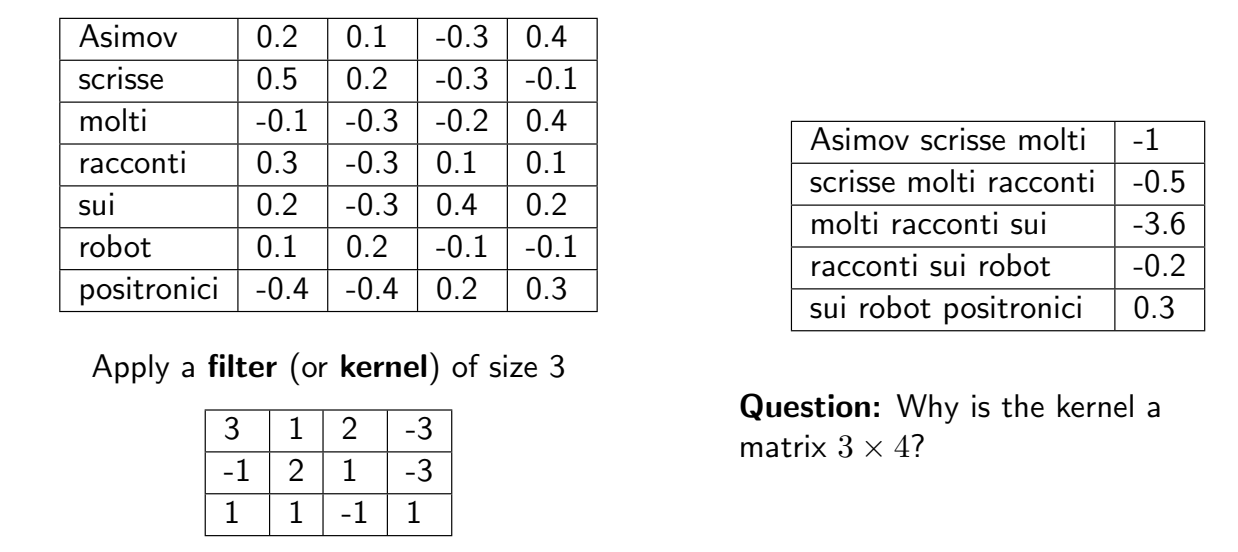
\includegraphics[keepaspectratio]{figure/fig_e92cb21c04ffd1e8.png}}
\caption{Slide 8 --- Feature delle parole, filtro e risultati}
\end{figure}
% END F04-B0034

% BEGIN F04-B0035
Da 7 posizioni si ottengono \(7-3+1=5\) uscite con stride 1 e senza padding. Un filtro produce un canale; per generare più feature si usano più filtri distinti.
% END F04-B0035

% BEGIN F04-B0036
Il conteggio per uno strato standard, con bias, è
% END F04-B0036

% BEGIN F04-B0037
\begin{center}
\begin{adjustbox}{max width=\linewidth}
$\displaystyle \boxed{P_{\mathrm{Conv1D}}=C_{\mathrm{out}}(kC_{\mathrm{in}}+1).}$
\end{adjustbox}
\end{center}
% END F04-B0037

% BEGIN F04-B0038
Si contano \(kC_{\mathrm{in}}\) pesi e un bias per filtro, poi si moltiplica per il numero di filtri. Con \(k=3\), \(C_{\mathrm{in}}=4\) e 8 filtri sono \(8(12+1)=104\) parametri; nell\textquotesingle esempio con un solo filtro senza bias sono 12 pesi. La lunghezza della sequenza non compare nel conteggio.
% END F04-B0038

% BEGIN F04-B0039
\begin{quote}
\textbf{Precisazione slide 5--6 --- Richiamo storico e significato di 1D}
\end{quote}
% END F04-B0039

% BEGIN F04-B0040
\begin{quote}
LeNet-5 è un riferimento storico importante, ma non segna la prima comparsa in assoluto delle idee convoluzionali. La distinzione 1D/2D riguarda il numero di assi lungo cui scorre il filtro; con più canali, un filtro 1D non è semplicemente un vettore di soli \(k\) scalari.
\end{quote}
% END F04-B0040

% BEGIN F04-B0041
\section{Dilatazione: ampliare la regione osservata senza nuovi pesi (slide 9)}\label{f04-r135}
% END F04-B0041

% BEGIN F04-B0042
Una finestra piccola coglie relazioni locali. Per osservare elementi più lontani si può introdurre una \textbf{dilatazione}: i pesi vengono applicati a posizioni distanziate, lasciando intervalli fra un campione e il successivo.
% END F04-B0042

% BEGIN F04-B0043
\begin{center}
\begin{adjustbox}{max width=\linewidth}
$\displaystyle \boxed{y_t=\sum_{i=0}^{k-1}x_{t-di}\omega_i,\qquad d\geq1.}$
\end{adjustbox}
\end{center}
% END F04-B0043

% BEGIN F04-B0044
\(d\) è il fattore di dilatazione, intero positivo. Nell\textquotesingle indice del campione si sostituisce il ritardo \(i\) con \(di\). Per \(k=3\):
% END F04-B0044

% BEGIN F04-B0045
\begin{center}
\begin{adjustbox}{max width=\linewidth}
$\displaystyle y_t=x_t\omega_0+x_{t-d}\omega_1+x_{t-2d}\omega_2.$
\end{adjustbox}
\end{center}
% END F04-B0045

% BEGIN F04-B0046
La distanza fra primo e ultimo campione è \((k-1)d\); contando entrambi gli estremi, l\textquotesingle ampiezza temporale coperta è
% END F04-B0046

% BEGIN F04-B0047
\begin{center}
\begin{adjustbox}{max width=\linewidth}
$\displaystyle \boxed{k_{\mathrm{eff}}=1+(k-1)d.}$
\end{adjustbox}
\end{center}
% END F04-B0047

% BEGIN F04-B0048
Con \(k=3,d=2\) si usano gli offset \(0,2,4\), quindi si copre un intervallo di 5 posizioni con \textbf{tre} pesi per canale. Con \(d=4\), gli offset sono \(0,4,8\) e l\textquotesingle intervallo è lungo 9. La dilatazione non trasforma il kernel in un filtro denso di 5 o 9 pesi.
% END F04-B0048

% BEGIN F04-B0049
\begin{figure}[H]
\centering
\pandocbounded{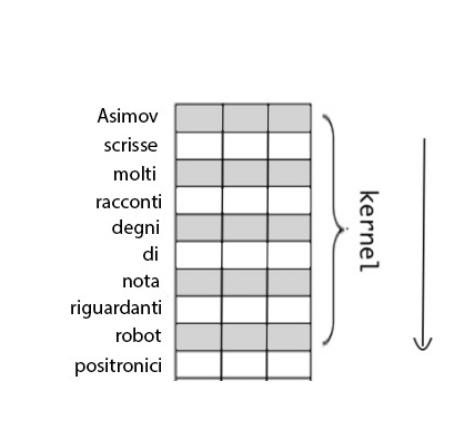
\includegraphics[keepaspectratio]{figure/fig_81e8f4cdd2640e61.png}}
\caption{Slide 9 --- Campioni distanziati nella finestra dilatata}
\end{figure}
% END F04-B0049

% BEGIN F04-B0050
La differenza dallo \textbf{stride} è essenziale:
% END F04-B0050

% BEGIN F04-B0051
\begin{itemize}
\tightlist
\item
  la dilatazione modifica la distanza fra i punti letti all\textquotesingle interno della finestra;
\item
  lo stride modifica la distanza fra le posizioni di uscita a cui si applica la finestra.
\end{itemize}
% END F04-B0051

% BEGIN F04-B0052
Si può usare \(d>1\) mantenendo stride 1, senza sottocampionare la griglia delle uscite. È utile quando un evento molto breve, quasi impulsivo, non deve scomparire fra due posizioni campionate. Anche nelle immagini un sottocampionamento può perdere dettagli: la differenza è una scelta legata al compito, non una garanzia assoluta dei dati visivi.
% END F04-B0052

% BEGIN F04-B0053
Un livello dilatato legge solo alcuni punti della sua griglia di ingresso; se i livelli precedenti hanno già combinato osservazioni locali, quei punti rappresentano però regioni più estese. Saltare una posizione intermedia a un livello profondo non equivale necessariamente a scartare il corrispondente dato grezzo dall\textquotesingle intera rete.
% END F04-B0053

% BEGIN F04-B0054
\begin{quote}
\textbf{Precisazione slide 9--11 --- Indici, stride e crescita del campo recettivo}
\end{quote}
% END F04-B0054

% BEGIN F04-B0055
\begin{quote}
Con kernel di tre elementi e dilatazione 2 si leggono, in avanti, le posizioni 1, 3 e 5, non 1, 3 e 6. La dilatazione non richiede stride 2. Inoltre anche convoluzioni non dilatate a stride 1 fanno crescere il campo recettivo quando si impilano livelli: la dilatazione ne accelera la crescita.
\end{quote}
% END F04-B0055

% BEGIN F04-B0056
\section{Causalità: non leggere un futuro indisponibile (slide 10)}\label{f04-r165}
% END F04-B0056

% BEGIN F04-B0057
Per produrre un risultato al tempo \(t\) usando soltanto ciò che è già disponibile, una convoluzione deve dipendere da ingressi con indice \textbf{minore o uguale a \(t\)}. Questo è il vincolo di \textbf{causalità temporale}. Una finestra centrata su \(t\) che leggesse anche \(t+1\) o \(t+2\) violerebbe il vincolo.
% END F04-B0057

% BEGIN F04-B0058
La formula dilatata precedente è già scritta in forma causale, perché usa \(t,t-d,\ldots,t-(k-1)d\). All\textquotesingle inizio mancano alcuni valori passati: un padding soltanto a sinistra permette di trattarli senza leggere valori futuri. Per stride 1 e uscita lunga quanto l\textquotesingle ingresso:
% END F04-B0058

% BEGIN F04-B0059
\begin{center}
\begin{adjustbox}{max width=\linewidth}
$\displaystyle \boxed{P_{\mathrm{sinistra}}=(k-1)d,\qquad P_{\mathrm{destra}}=0.}$
\end{adjustbox}
\end{center}
% END F04-B0059

% BEGIN F04-B0060
Infatti il kernel effettivo è lungo \(k_{\mathrm{eff}}=1+(k-1)d\). Partendo da una sequenza di lunghezza \(T\):
% END F04-B0060

% BEGIN F04-B0061
\begin{center}
\begin{adjustbox}{max width=\linewidth}
$\displaystyle 
\begin{aligned}
T_{\mathrm{out}}&=T+P_{\mathrm{sinistra}}-k_{\mathrm{eff}}+1
&&\text{conteggio delle finestre a stride 1},\\
&=T+(k-1)d-[1+(k-1)d]+1=T
&&\text{sostituzione e semplificazione}.
\end{aligned}
$
\end{adjustbox}
\end{center}
% END F04-B0061

% BEGIN F04-B0062
Con \(k=3,d=2\) servono quattro valori di padding a sinistra. Se i pesi sono tutti 1 e i primi dati sono \((1,2,3,4,5)\), l\textquotesingle uscita al terzo istante usa \(x_3+x_1+x_{-1}=3+1+0=4\); al quinto usa \(x_5+x_3+x_1=5+3+1=9\). Nessuno dei due risultati richiede valori futuri.
% END F04-B0062

% BEGIN F04-B0063
\begin{figure}[H]
\centering
\pandocbounded{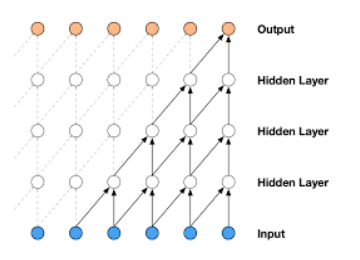
\includegraphics[keepaspectratio]{figure/fig_42545ec9e242409b.png}}
\caption{Slide 10 --- Collegamenti causali fra i livelli}
\end{figure}
% END F04-B0063

% BEGIN F04-B0064
La causalità indica un vincolo di disponibilità dell\textquotesingle informazione, non una prova che un ingresso causi fisicamente un evento. Inoltre \(y_t\) può dipendere da \(x_t\): se il compito consiste nel prevedere il valore ancora sconosciuto \(x_t\), occorre allineare i target rispetto agli ingressi, per esempio prevedendo \(x_{t+1}\) dai dati fino a \(t\). Causalità del filtro e definizione della previsione devono essere coerenti.
% END F04-B0064

% BEGIN F04-B0065
\section{Temporal Convolutional Network: gerarchia e blocchi residui (slide 11)}\label{f04-r190}
% END F04-B0065

% BEGIN F04-B0066
Una \textbf{TCN} combina convoluzioni causali e dilatate in una gerarchia. La figura mostra kernel di ampiezza 3 e dilatazioni \(1,2,4\): salendo di livello, ogni elemento riassume una porzione più lunga della sequenza originale.
% END F04-B0066

% BEGIN F04-B0067
\begin{figure}[H]
\centering
\pandocbounded{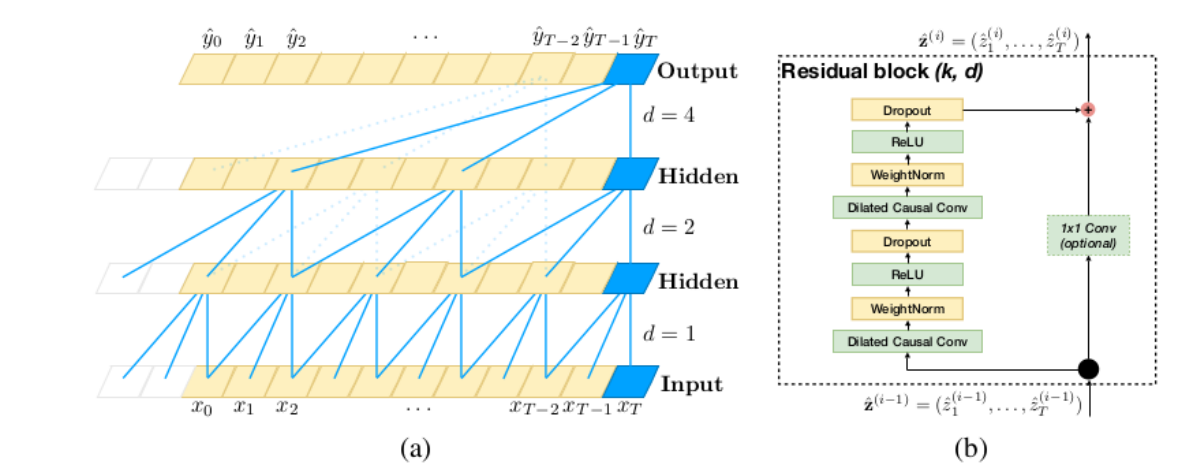
\includegraphics[keepaspectratio]{figure/fig_1eb346b8204e8b28.png}}
\caption{Slide 11 --- Crescita del campo recettivo e blocco residuo TCN}
\end{figure}
% END F04-B0067

% BEGIN F04-B0068
\subsection{Campo recettivo lungo la sequenza (slide 11)}\label{f04-r196}
% END F04-B0068

% BEGIN F04-B0069
Riprendiamo da \hyperref[fonte02]{reti convoluzionali} il campo recettivo \(r_\ell\) e la distanza \(j_\ell\) fra centri di uscite adiacenti, misurati sull\textquotesingle ingresso originale. Con kernel \(k_\ell\), dilatazione \(d_\ell\) e stride \(s_\ell\):
% END F04-B0069

% BEGIN F04-B0070
\begin{center}
\begin{adjustbox}{max width=\linewidth}
$\displaystyle \boxed{\begin{aligned}
r_\ell&=r_{\ell-1}+(k_\ell-1)d_\ell j_{\ell-1},\\
j_\ell&=s_\ell j_{\ell-1},\qquad r_0=j_0=1.
\end{aligned}}$
\end{adjustbox}
\end{center}
% END F04-B0070

% BEGIN F04-B0071
Fra primo e ultimo punto della finestra ci sono \(k_\ell-1\) intervalli; ognuno vale \(d_\ell\) posizioni della griglia precedente, distanziate di \(j_{\ell-1}\) sull\textquotesingle ingresso. Da qui il termine aggiunto. Lo stride determina invece la nuova distanza fra uscite.
% END F04-B0071

% BEGIN F04-B0072
Con stride sempre 1 si mantiene \(j_\ell=1\). Per i tre livelli della figura:
% END F04-B0072

% BEGIN F04-B0073
\begin{longtable}[]{@{}lrrlr@{}}
\toprule\noalign{}
Livello & \(k\) & \(d\) & Calcolo & Campo recettivo \\
\midrule\noalign{}
\endhead
\bottomrule\noalign{}
\endlastfoot
Ingresso & --- & --- & Valore iniziale & 1 \\
1 & 3 & 1 & \(1+2\cdot1\) & 3 \\
2 & 3 & 2 & \(3+2\cdot2\) & 7 \\
3 & 3 & 4 & \(7+2\cdot4\) & 15 \\
\end{longtable}
% END F04-B0073

% BEGIN F04-B0074
Un\textquotesingle uscita finale può quindi dipendere da 15 istanti, pur usando kernel di soli tre campioni. I salti di un livello si combinano con le regioni già elaborate dal precedente.
% END F04-B0074

% BEGIN F04-B0075
\subsection{Che cosa contiene il blocco reale (slide 11)}\label{f04-r218}
% END F04-B0075

% BEGIN F04-B0076
Il blocco a destra della figura comprende due sequenze convoluzione causale dilatata → normalizzazione dei pesi → ReLU → dropout, oltre a una connessione residua. La \textbf{WeightNorm} riguarda i pesi: non è la BatchNorm sulle attivazioni di \hyperref[fonte02]{reti convoluzionali} e non viene qui sviluppata matematicamente.
% END F04-B0076

% BEGIN F04-B0077
La shortcut somma ingresso e ramo trasformato. Se i canali non coincidono, una convoluzione \(1\times1\) può adattarli. È la stessa condizione di compatibilità delle forme già incontrata con ResNet: i due rami vengono calcolati e sommati, senza scegliere quale eseguire.
% END F04-B0077

% BEGIN F04-B0078
Il disegno a sinistra conta \textbf{una convoluzione per livello}. Se invece si impilano tre blocchi con due convoluzioni ciascuno alle dilatazioni \(1,2,4\), il campo recettivo massimo del ramo profondo diventa \(1+2\cdot2(1+2+4)=29\). Il conteggio va fatto sulle operazioni effettive, non confondendo un blocco con una singola convoluzione.
% END F04-B0078

% BEGIN F04-B0079
Le convoluzioni possono elaborare sequenze di lunghezza diversa mantenendo gli stessi pesi. Una eventuale testa densa su una concatenazione completa può tuttavia reintrodurre il vincolo di lunghezza fissa; la flessibilità dell\textquotesingle estrattore non rende automaticamente flessibile qualsiasi classificatore finale.
% END F04-B0079

% BEGIN F04-B0080
\section{Caso di studio finanziario: dati, baseline e risultati (slide 12--13)}\label{f04-r228}
% END F04-B0080

% BEGIN F04-B0081
Il caso illustrato combina tre fonti: valori giornalieri dell\textquotesingle indice DJIA, titoli di notizie e conoscenza strutturata da grafi. Il compito è classificare il movimento successivo come rialzo o ribasso. Le feature provenienti da più fonti possono essere allineate e affiancate lungo l\textquotesingle asse dei canali, mantenendo la struttura temporale.
% END F04-B0081

% BEGIN F04-B0082
\begin{figure}[H]
\centering
\pandocbounded{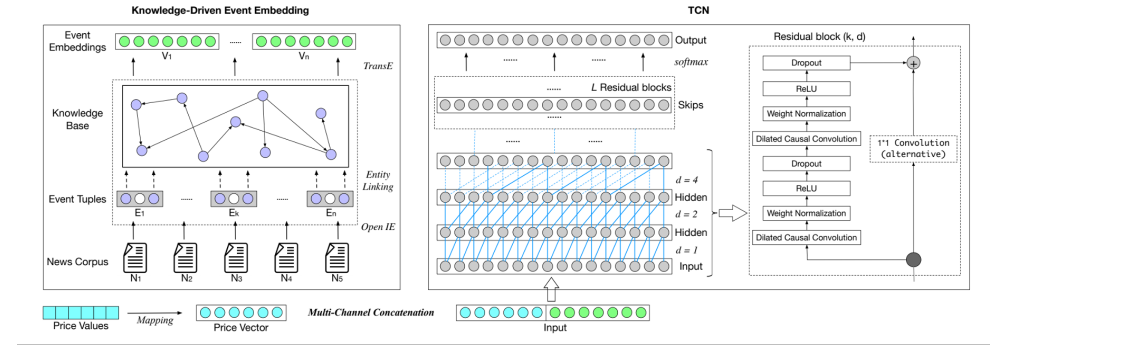
\includegraphics[keepaspectratio]{figure/fig_e3790bfdb3d922aa.png}}
\caption{Slide 12 --- Fusione delle fonti e classificazione del movimento}
\end{figure}
% END F04-B0082

% BEGIN F04-B0083
Aggiungere canali non cambia il principio convoluzionale, ma \textbf{aumenta i pesi del filtro}, perché ciascun filtro deve coprire anche le nuove feature. Non significa inserire dati eterogenei senza prima renderli rappresentabili e temporalmente coerenti. La costruzione dei grafi e degli embedding del caso di studio non è sviluppata.
% END F04-B0083

% BEGIN F04-B0084
\begin{figure}[H]
\centering
\pandocbounded{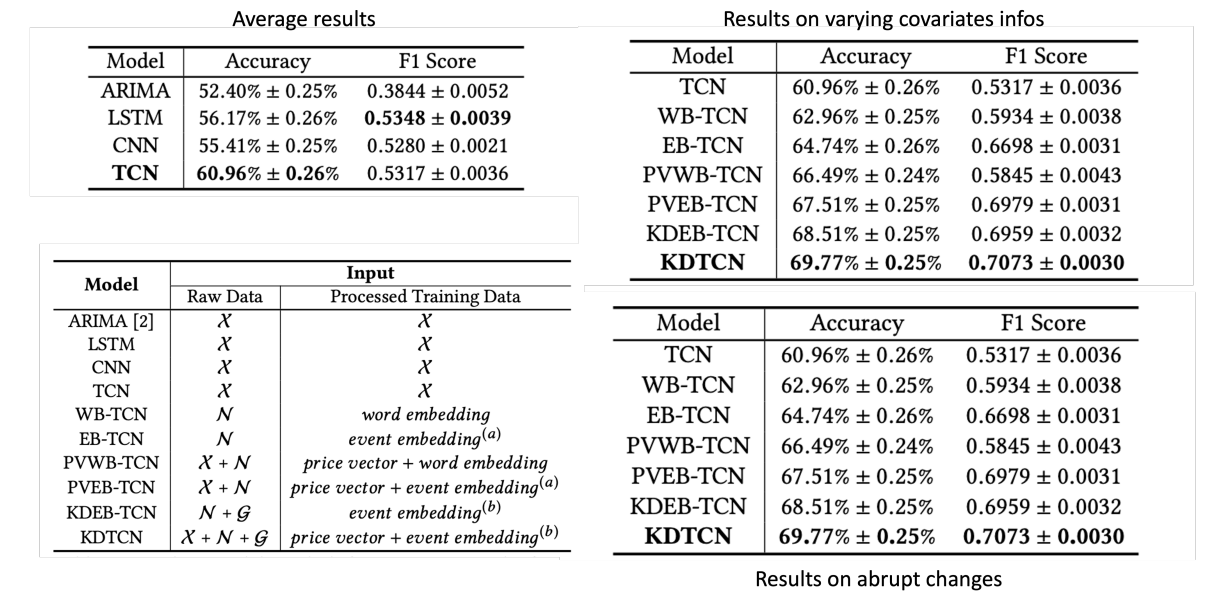
\includegraphics[keepaspectratio]{figure/fig_3965d448634bbfda.png}}
\caption{Slide 13 --- Tabelle dei risultati e confronto delle feature}
\end{figure}
% END F04-B0084

% BEGIN F04-B0085
\begin{longtable}[]{@{}lrr@{}}
\toprule\noalign{}
Modello, confronto iniziale & Accuracy media & F1 \\
\midrule\noalign{}
\endhead
\bottomrule\noalign{}
\endlastfoot
ARIMA & \(52.40\%\pm0.25\%\) & \(0.3844\pm0.0052\) \\
LSTM & \(56.17\%\pm0.26\%\) & \(0.5348\pm0.0039\) \\
CNN & \(55.41\%\pm0.25\%\) & \(0.5280\pm0.0021\) \\
TCN & \(60.96\%\pm0.26\%\) & \(0.5317\pm0.0036\) \\
\end{longtable}
% END F04-B0085

% BEGIN F04-B0086
La TCN migliora l\textquotesingle accuracy della LSTM di \(60.96-56.17=4.79\) \textbf{punti percentuali}. La F1 è però leggermente più bassa: \(0.5317<0.5348\). Dire che un modello è migliore richiede quindi di specificare la metrica, oltre al dataset e al protocollo.
% END F04-B0086

% BEGIN F04-B0087
Nella tabella con diverse covariate, il modello KDTCN che combina prezzi, notizie e conoscenza strutturata raggiunge \(69.77\%\pm0.25\%\) di accuracy e \(0.7073\pm0.0030\) di F1. La tabella sui cambiamenti bruschi riporta lo stesso valore centrale di accuracy, con dispersione \(0.24\%\): le due tabelle non vanno fuse attribuendo loro un\textquotesingle identica condizione sperimentale.
% END F04-B0087

% BEGIN F04-B0088
Un\textquotesingle accuracy attorno al 60\% è un risultato del caso studiato, non una garanzia di previsione finanziaria o redditività. Una baseline casuale al 50\% di accuracy presuppone una scelta binaria equiprobabile; per le metriche e il dataset reale servono confronti appropriati. In particolare una F1 pari a 0.5 non è una baseline universale: dipende da prevalenza della classe positiva e regola di predizione. Il significato delle metriche si collega a manuale introduttivo di Machine Learning (documento separato).
% END F04-B0088

% BEGIN F04-B0089
\section{TCN e RNN: memoria, parallelismo e spiegazioni (slide 14)}\label{f04-r251}
% END F04-B0089

% BEGIN F04-B0090
Una RNN conserva uno stato di dimensione fissata. Riassumere 20 osservazioni o 4000 osservazioni in 128 numeri pone un diverso carico alla stessa rappresentazione: è l\textquotesingle idea del \textbf{riassunto con perdita} discussa in \hyperref[fonte03]{reti ricorrenti}. Una TCN conserva invece mappe di feature indicizzate lungo la sequenza, fino a un\textquotesingle eventuale aggregazione finale.
% END F04-B0090

% BEGIN F04-B0091
La maggiore lunghezza delle mappe ha un costo di memoria. A parità di canali, raddoppiare la lunghezza raddoppia le attivazioni di un livello che la conserva. Inoltre una TCN di profondità fissata vede un campo recettivo finito: accettare ingressi più lunghi non amplia automaticamente la storia osservabile da ogni uscita.
% END F04-B0091

% BEGIN F04-B0092
Il vantaggio computazionale è l\textquotesingle assenza di una ricorrenza che imponga di completare \(h_t\) prima di calcolare \(h_{t+1}\). Le posizioni di una convoluzione nello stesso livello possono essere calcolate in parallelo, oltre ai filtri; rimane la dipendenza fra livelli successivi.
% END F04-B0092

% BEGIN F04-B0093
Per l\textquotesingle apprendimento si applica la backpropagation al grafo convoluzionale, senza srotolare una cella ricorrente per ogni istante. \textbf{La backpropagation non scompare.} Le connessioni residue e la struttura della rete possono facilitarla; non eliminano ogni possibile instabilità.
% END F04-B0093

% BEGIN F04-B0094
\begin{quote}
\textbf{Errata slide 14 --- Nessuna garanzia assoluta sui gradienti}
\end{quote}
% END F04-B0094

% BEGIN F04-B0095
\begin{quote}
L\textquotesingle affermazione «no vanishing/exploding gradients» è troppo forte. La TCN evita la specifica catena ricorrente attraverso tutti gli istanti, ma una rete convoluzionale profonda può comunque avere gradienti che svaniscono o esplodono. I risultati favorevoli rispetto a LSTM e GRU descrivono confronti sperimentali, non una superiorità universale.
\end{quote}
% END F04-B0095

% BEGIN F04-B0096
La struttura convoluzionale consente anche di adattare strumenti di localizzazione come Grad-CAM per evidenziare porzioni della sequenza associate a una decisione. Non segue che le RNN siano impossibili da analizzare: anche un grafo ricorrente srotolato può essere studiato con metodi di attribuzione. Il richiamo alla spiegabilità indica una possibilità pratica delle TCN, senza sviluppare qui l\textquotesingle algoritmo Grad-CAM né trasformare una mappa di attribuzione in una prova causale.
% END F04-B0096

% BEGIN F04-B0097
\chapter{Transformer}\label{fonte04}
% END F04-B0097

% BEGIN F04-B0098
\begin{indiceargomento}
\item \hyperref[f04-r266]{Dai collegamenti regolari alle relazioni dipendenti dal contenuto (slide 15--18)}
\item \hyperref[f04-r276]{Encoder e decoder: ruoli e perimetro (slide 19--20)}
\item \hyperref[f04-r296]{Dall\textquotesingle ingresso ai token e alla posizione (slide 21)}
\item \hyperref[f04-r325]{Blocco encoder: attention, MLP, residui e normalizzazione (slide 22--25)}
\item \hyperref[f04-r394]{Layer Normalization: normalizzare le feature del singolo token (slide 26--28)}
\item \hyperref[f04-r487]{Attention: ricostruire ogni token dal contesto (slide 29--32)}
\item \hyperref[f04-r540]{Query, key e value: tre proiezioni dello stesso ingresso (slide 33)}
\item \hyperref[f04-r596]{Single-head attention: dal confronto alla somma pesata (slide 34)}
\item \hyperref[f04-r716]{Multi-Head Attention: più confronti in parallelo (slide 35--36)}
\item \hyperref[f04-r766]{Dalla sequenza di rappresentazioni alla classificazione (slide 37--38)}
\item \hyperref[f04-r821]{TCN e Transformer: confronto, modalità e costi (slide 39--41)}
\item \hyperref[f04-r898]{Confine della spiegazione e materiale rinviato (slide 42--60)}
\item \hyperref[f04-r907]{Riepilogo delle forme e delle formule (slide 5--41)}
\item \hyperref[f04-r933]{Errata e precisazioni principali (slide 5--41)}
\end{indiceargomento}
% END F04-B0098

% BEGIN F04-B0099
\section{Dai collegamenti regolari alle relazioni dipendenti dal contenuto (slide 15--18)}\label{f04-r266}
% END F04-B0099

% BEGIN F04-B0100
Le convoluzioni impongono un\textquotesingle organizzazione regolare dei collegamenti. La dilatazione può ampliare la distanza fra campioni, ma la regola dei salti è fissata dall\textquotesingle architettura: una volta scelti kernel e dilatazioni, le posizioni potenzialmente collegate sono determinate.
% END F04-B0100

% BEGIN F04-B0101
Molte dipendenze non seguono una distanza costante. In una frase, un nome può essere collegato al suo articolo e poi richiamato molto più avanti; fra i due possono comparire quantità diverse di parole. Nel codice, la chiusura di un ciclo \texttt{for} è collegata alla sua apertura, ma la distanza cambia con la lunghezza del blocco. Non basta quindi scegliere un unico salto periodico adatto a tutti gli esempi.
% END F04-B0101

% BEGIN F04-B0102
La domanda è: \textbf{si possono calcolare, per ogni ingresso, coefficienti che descrivano quali elementi mettere in relazione?} L\textquotesingle attention costruisce proprio questi coefficienti. Non cambia i parametri del modello durante il forward: usa parametri già appresi per produrre relazioni che dipendono dai dati correnti.
% END F04-B0102

% BEGIN F04-B0103
Il Transformer presentato in \emph{Attention Is All You Need} del 2017 combina meccanismi di attention con trasformazioni lineari, MLP, connessioni residue e normalizzazione. Non è una rete priva di struttura o di bias induttivi: cambia il modo di far interagire le posizioni, rendendolo dipendente dal contenuto.
% END F04-B0103

% BEGIN F04-B0104
\section{Encoder e decoder: ruoli e perimetro (slide 19--20)}\label{f04-r276}
% END F04-B0104

% BEGIN F04-B0105
L\textquotesingle architettura illustrata ha due rami:
% END F04-B0105

% BEGIN F04-B0106
\begin{itemize}
\tightlist
\item
  l\textquotesingle{}\textbf{encoder} trasforma una sequenza in una sequenza di rappresentazioni;
\item
  il \textbf{decoder} costruisce una sequenza di uscita, eventualmente condizionandosi anche alle rappresentazioni dell\textquotesingle encoder.
\end{itemize}
% END F04-B0106

% BEGIN F04-B0107
\begin{figure}[H]
\centering
\pandocbounded{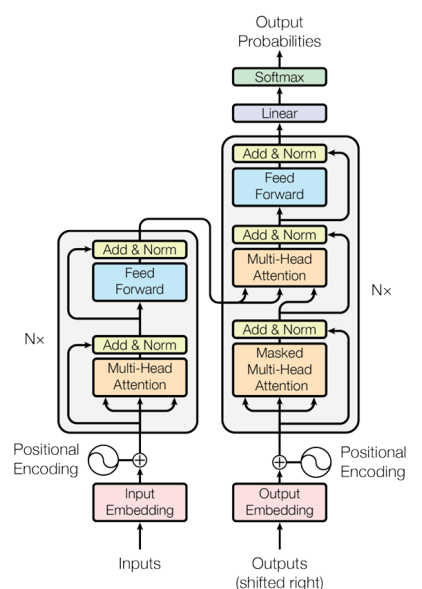
\includegraphics[keepaspectratio]{figure/fig_cac00fb9b59eba03.png}}
\caption{Slide 19 --- Architettura encoder--decoder di riferimento}
\end{figure}
% END F04-B0107

% BEGIN F04-B0108
Nella traduzione, l\textquotesingle encoder rappresenta la frase nella lingua di partenza e il decoder produce quella nella lingua di arrivo. Per classificare una frase come positiva o negativa può bastare un encoder con una testa di classificazione. Una rete di generazione può invece essere basata sul solo decoder, producendo progressivamente nuovi elementi condizionati al contesto.
% END F04-B0108

% BEGIN F04-B0109
La coppia encoder--decoder non serve soltanto a cambiare modalità: una traduzione fra lingue rimane interamente testuale. Analogamente, usare token di modalità differenti richiede rappresentazioni e addestramento coerenti, non necessariamente proprio lo schema completo della figura.
% END F04-B0109

% BEGIN F04-B0110
Il prompt «Elon Musk che mangia un Kinder Bueno» illustra il principio di \textbf{condizionare} una generazione di immagini con una descrizione testuale: il testo deve influire sul contenuto prodotto. L\textquotesingle esempio non identifica l\textquotesingle architettura esatta di ogni sistema di generazione d\textquotesingle immagini, né implica che tutti seguano il decoder testuale disegnato nella figura.
% END F04-B0110

% BEGIN F04-B0111
Il valore \(N=6\) riportato nelle slide è il numero di livelli della configurazione di riferimento, non una costante obbligatoria per ogni Transformer.
% END F04-B0111

% BEGIN F04-B0112
\begin{quote}
\textbf{Slide 20 --- Componenti non sviluppate in dettaglio}
\end{quote}
% END F04-B0112

% BEGIN F04-B0113
\begin{quote}
La trattazione si concentra sull\textquotesingle encoder. Del positional encoding viene data l\textquotesingle intuizione qualitativa; non vengono sviluppate le sue formule sinusoidali. Decoder, masking e cross-attention restano richiami di contesto: non si aggiungono le equazioni o la descrizione completa di questi moduli.
\end{quote}
% END F04-B0113

% BEGIN F04-B0114
\section{Dall\textquotesingle ingresso ai token e alla posizione (slide 21)}\label{f04-r296}
% END F04-B0114

% BEGIN F04-B0115
Per entrare nel Transformer, ogni elemento deve essere rappresentato mediante un vettore di dimensione fissata \(D=d_{\mathrm{model}}\). Con una riga per token:
% END F04-B0115

% BEGIN F04-B0116
\begin{center}
\begin{adjustbox}{max width=\linewidth}
$\displaystyle \boxed{X\in\mathbb R^{T\times D}.}$
\end{adjustbox}
\end{center}
% END F04-B0116

% BEGIN F04-B0117
\(T\) è il numero di token; \(D\) è il numero di feature di ogni token. Per esempio, 100 token con 10 feature danno una matrice \(100\times10\). Il blocco encoder descritto mantiene questa forma: non esegue pooling temporale fra un livello e il successivo.
% END F04-B0117

% BEGIN F04-B0118
\subsection{Tokenizzazione ed embedding sono passaggi distinti (slide 21)}\label{f04-r304}
% END F04-B0118

% BEGIN F04-B0119
Nel caso testuale, la \textbf{tokenizzazione} suddivide il testo in unità e le associa a identificativi; l\textquotesingle{}\textbf{embedding} associa agli identificativi dei vettori numerici. Nel linguaggio del calcolo, «token» può indicare anche il vettore che rappresenta quell\textquotesingle unità, ma è utile distinguere i due passaggi.
% END F04-B0119

% BEGIN F04-B0120
Una parola non corrisponde necessariamente a un solo token: un tokenizer può produrre sottoparole o altre unità. La corrispondenza «un ingresso, un vettore» descrive la sequenza dopo che quelle unità sono state definite. Il numero di feature per vettore rimane fissato, mentre il numero di vettori può variare.
% END F04-B0120

% BEGIN F04-B0121
Word2Vec è un esempio richiamato per l\textquotesingle idea di rappresentare parole con vettori. Non occorre che i vettori siano progettati manualmente; possono essere appresi e possono provenire da un modello già disponibile. Il modulo di embedding di un Transformer può anche essere addestrato insieme al resto della rete. Non si deve estendere al suo embedding l\textquotesingle idea che il tokenizer discreto venga normalmente scelto prima del training del modello.
% END F04-B0121

% BEGIN F04-B0122
\begin{quote}
\textbf{Precisazione slide 21 --- Token, parola e rappresentazione appresa}
\end{quote}
% END F04-B0122

% BEGIN F04-B0123
\begin{quote}
«Un token per parola» è una semplificazione dell\textquotesingle esempio, non una proprietà generale. Tokenizzazione ed embedding non sono la stessa operazione: la prima definisce le unità e gli identificativi, il secondo costruisce i vettori e può ricevere gradienti durante l\textquotesingle addestramento end-to-end.
\end{quote}
% END F04-B0123

% BEGIN F04-B0124
\subsection{Perché aggiungere la posizione (slide 21)}\label{f04-r315}
% END F04-B0124

% BEGIN F04-B0125
Confrontare il contenuto dei token, da solo, non assegna un significato alla loro posizione nella frase. Per rendere accessibile l\textquotesingle ordine si introduce una rappresentazione della posizione, qui descritta come un vettore aggiunto alle feature:
% END F04-B0125

% BEGIN F04-B0126
\begin{center}
\begin{adjustbox}{max width=\linewidth}
$\displaystyle \boxed{x_t=e_t+p_t,\qquad e_t,p_t,x_t\in\mathbb R^D.}$
\end{adjustbox}
\end{center}
% END F04-B0126

% BEGIN F04-B0127
\(e_t\) è l\textquotesingle embedding del contenuto e \(p_t\) codifica la posizione. La somma è possibile perché le forme coincidono. Per esempio, nell\textquotesingle illustrazione più semplice si potrebbe aggiungere l\textquotesingle indice a ogni feature: con \(e_1=(0.2,0.4)\) e \(p_1=(1,1)\) si ottiene \(x_1=(1.2,1.4)\); alla seconda posizione si potrebbe usare \(p_2=(2,2)\). È un esempio intuitivo, non la codifica sinusoidale dell\textquotesingle architettura di riferimento né una raccomandazione progettuale.
% END F04-B0127

% BEGIN F04-B0128
Nel caso descritto, le funzioni di posizione sono fissate; altri dettagli di progettazione non sono necessari per seguire il blocco encoder. Il collegamento con le feature cicliche di \hyperref[fonte03]{reti ricorrenti} è l\textquotesingle uso di funzioni numeriche per rappresentare una struttura dell\textquotesingle indice, senza identificare i due meccanismi.
% END F04-B0128

% BEGIN F04-B0129
\section{Blocco encoder: attention, MLP, residui e normalizzazione (slide 22--25)}\label{f04-r325}
% END F04-B0129

% BEGIN F04-B0130
Il blocco contiene due trasformazioni principali: \textbf{Multi-Head Attention} e \textbf{Feed-Forward Network}. Dopo ciascuna si somma l\textquotesingle ingresso del sottoblocco e si applica LayerNorm. L\textquotesingle ordine mostrato è quindi quello con normalizzazione successiva alla somma.
% END F04-B0130

% BEGIN F04-B0131
\begin{figure}[H]
\centering
\pandocbounded{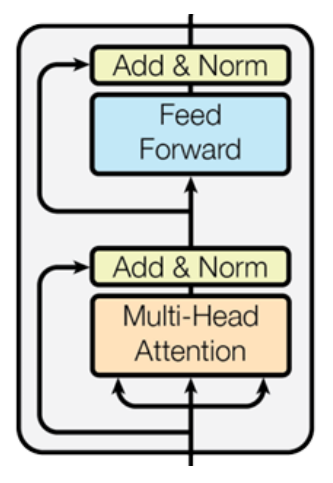
\includegraphics[keepaspectratio]{figure/fig_44aa361fa22c8d07.png}}
\caption{Slide 25 --- Blocco encoder con due connessioni residue}
\end{figure}
% END F04-B0131

% BEGIN F04-B0132
Scrivendo \(\operatorname{MHA}\) per la multi-head attention e \(\operatorname{FFN}\) per il piccolo MLP:
% END F04-B0132

% BEGIN F04-B0133
\begin{center}
\begin{adjustbox}{max width=\linewidth}
$\displaystyle \boxed{\begin{aligned}
Y&=\operatorname{LN}_1\bigl(X+\operatorname{MHA}(X)\bigr),\\
B&=\operatorname{LN}_2\bigl(Y+\operatorname{FFN}(Y)\bigr).
\end{aligned}}$
\end{adjustbox}
\end{center}
% END F04-B0133

% BEGIN F04-B0134
\(X,Y,B\) hanno forma \(T\times D\). Perché le somme siano definite, anche MHA e FFN devono restituire \(T\times D\). Le due LayerNorm hanno propri parametri. La forma resta uguale, ma il contenuto dei vettori cambia: ogni livello può affinare le rappresentazioni.
% END F04-B0134

% BEGIN F04-B0135
\pandocbounded{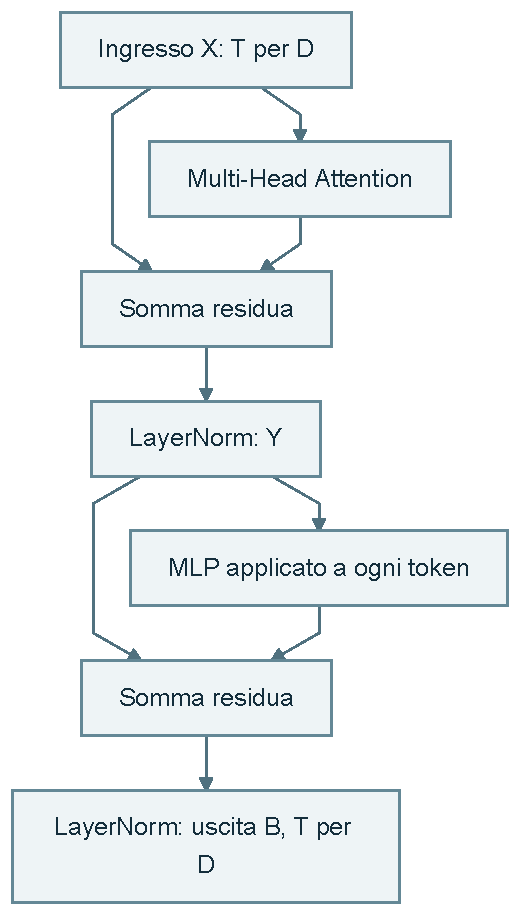
\includegraphics[keepaspectratio]{figure/diagramma_f04_02.pdf}}
% END F04-B0135

% BEGIN F04-B0136
\subsection{MLP per token e condivisione dei pesi (slide 23--25)}\label{f04-r352}
% END F04-B0136

% BEGIN F04-B0137
Il feed-forward comprende due trasformazioni lineari con ReLU in mezzo. Per un token riga \(y_t\in\mathbb R^{1\times D}\):
% END F04-B0137

% BEGIN F04-B0138
\begin{center}
\begin{adjustbox}{max width=\linewidth}
$\displaystyle \boxed{\operatorname{FFN}(y_t)=\operatorname{ReLU}(y_tW_1+b_1)W_2+b_2.}$
\end{adjustbox}
\end{center}
% END F04-B0138

% BEGIN F04-B0139
La dimensione interna \(F\) può essere diversa da \(D\):
% END F04-B0139

% BEGIN F04-B0140
\begin{longtable}[]{@{}ll@{}}
\toprule\noalign{}
Quantità & Forma \\
\midrule\noalign{}
\endhead
\bottomrule\noalign{}
\endlastfoot
\(W_1\) & \(D\times F\) \\
\(b_1\) & \(1\times F\) \\
\(y_tW_1+b_1\) & \(1\times F\) \\
\(W_2\) & \(F\times D\) \\
\(b_2\) & \(1\times D\) \\
\(\operatorname{FFN}(y_t)\) & \(1\times D\) \\
\end{longtable}
% END F04-B0140

% BEGIN F04-B0141
Il calcolo prima proietta da \(D\) a \(F\), applica la non linearità e poi torna da \(F\) a \(D\). \textbf{Lo stesso MLP, con gli stessi pesi, viene applicato a ogni posizione.} «Indipendentemente» significa che questa operazione non mescola token differenti, non che ogni token abbia un MLP distinto. Le posizioni possono essere elaborate in parallelo.
% END F04-B0141

% BEGIN F04-B0142
Per \(D=2,F=3\), con bias nulli:
% END F04-B0142

% BEGIN F04-B0143
\begin{center}
\begin{adjustbox}{max width=\linewidth}
$\displaystyle y_t=\begin{bmatrix}1&-1\end{bmatrix},\quad
W_1=\begin{bmatrix}1&0&-1\\0&1&1\end{bmatrix},\quad
W_2=\begin{bmatrix}2&0\\0&1\\1&1\end{bmatrix}.$
\end{adjustbox}
\end{center}
% END F04-B0143

% BEGIN F04-B0144
Si ottiene:
% END F04-B0144

% BEGIN F04-B0145
\begin{center}
\begin{adjustbox}{max width=\linewidth}
$\displaystyle 
\begin{aligned}
y_tW_1&=\begin{bmatrix}1&-1&-2\end{bmatrix}
&&\text{primo prodotto riga per matrice},\\
\operatorname{ReLU}(y_tW_1)&=\begin{bmatrix}1&0&0\end{bmatrix}
&&\text{soglia a zero},\\
\operatorname{FFN}(y_t)&=\begin{bmatrix}2&0\end{bmatrix}
&&\text{seconda proiezione},\\
y_t+\operatorname{FFN}(y_t)&=\begin{bmatrix}3&-1\end{bmatrix}
&&\text{somma residua prima della normalizzazione}.
\end{aligned}
$
\end{adjustbox}
\end{center}
% END F04-B0145

% BEGIN F04-B0146
Il MLP ha dimensione finale uguale all\textquotesingle ingresso pur cambiando la dimensione interna. La connessione residua aggiunge il contributo diretto, come in \hyperref[fonte02]{reti convoluzionali}; non sostituisce la trasformazione né ne evita il calcolo. Il ruolo dell\textquotesingle attention sarà invece quello di mescolare informazioni fra token.
% END F04-B0146

% BEGIN F04-B0147
\section{Layer Normalization: normalizzare le feature del singolo token (slide 26--28)}\label{f04-r394}
% END F04-B0147

% BEGIN F04-B0148
La \textbf{Layer Normalization}, o \textbf{LayerNorm}, controlla centro e scala delle attivazioni \textbf{all\textquotesingle interno di ogni token}. Su un tensore di forma \(N\times T\times D\), qui si aggrega l\textquotesingle ultimo asse \(D\): ogni coppia campione--posizione ha le proprie statistiche.
% END F04-B0148

% BEGIN F04-B0149
Per un token \(x\in\mathbb R^D\), con vettori scritti qui per componenti:
% END F04-B0149

% BEGIN F04-B0150
\begin{center}
\begin{adjustbox}{max width=\linewidth}
$\displaystyle \boxed{\begin{aligned}
\mu&=\frac1D\sum_{j=1}^{D}x_j,\\
v&=\frac1D\sum_{j=1}^{D}(x_j-\mu)^2,\\
\widehat x_j&=\frac{x_j-\mu}{\sqrt{v+\epsilon}},\\
y_j&=\gamma_j\widehat x_j+\beta_j.
\end{aligned}}$
\end{adjustbox}
\end{center}
% END F04-B0150

% BEGIN F04-B0151
\(\mu,v\) sono scalari calcolati dal token corrente; \(\epsilon>0\) è una costante di stabilità. I vettori \(\gamma,\beta\in\mathbb R^D\) sono apprendibili e condivisi fra le posizioni per lo stesso modulo. In uscita rimangono \(D\) componenti.
% END F04-B0151

% BEGIN F04-B0152
\subsection{Da dove vengono i passaggi (slide 26--27)}\label{f04-r409}
% END F04-B0152

% BEGIN F04-B0153
La sottrazione della media centra gli scarti:
% END F04-B0153

% BEGIN F04-B0154
\begin{center}
\begin{adjustbox}{max width=\linewidth}
$\displaystyle 
\begin{aligned}
\frac1D\sum_j(x_j-\mu)
&=\frac1D\sum_jx_j-\frac1D\sum_j\mu
&&\text{linearità della somma},\\
&=\mu-\mu=0
&&\text{definizione della media}.
\end{aligned}
$
\end{adjustbox}
\end{center}
% END F04-B0154

% BEGIN F04-B0155
La divisione per la deviazione standard stabilizzata controlla la scala. Poiché \(\widehat x\) ha media zero:
% END F04-B0155

% BEGIN F04-B0156
\begin{center}
\begin{adjustbox}{max width=\linewidth}
$\displaystyle 
\begin{aligned}
\operatorname{var}(\widehat x)
&=\frac1D\sum_j\frac{(x_j-\mu)^2}{v+\epsilon},\\
&=\frac{v}{v+\epsilon}.
\end{aligned}
$
\end{adjustbox}
\end{center}
% END F04-B0156

% BEGIN F04-B0157
Questa varianza è vicina a 1 quando \(v\) è grande rispetto a \(\epsilon\), non identicamente 1. Se tutte le componenti coincidono, \(v=0\) e gli scarti normalizzati sono zero; \(\epsilon\) evita la divisione per zero. Un esempio con componenti tutte uguali a 5 produce quindi \(\widehat x=0\) e \(y=\beta\).
% END F04-B0157

% BEGIN F04-B0158
\begin{quote}
\textbf{Precisazione slide 26--27 --- Deviazione standard e stabilizzatore}
\end{quote}
% END F04-B0158

% BEGIN F04-B0159
\begin{quote}
Il denominatore della slide è \(\sigma+\epsilon\): \(\sigma\) va letto come \textbf{deviazione standard}, non varianza né covarianza. Qui si esplicita la convenzione comune \(\sqrt{v+\epsilon}\). Le due collocazioni di \(\epsilon\) sono varianti numeriche diverse: non si sostituisce l\textquotesingle una all\textquotesingle altra come identità algebrica. Dividere direttamente per \(v\) non realizza la standardizzazione descritta.
\end{quote}
% END F04-B0159

% BEGIN F04-B0160
\subsection{Gamma e beta: scala e traslazione apprendibili (slide 26--27)}\label{f04-r438}
% END F04-B0160

% BEGIN F04-B0161
La normalizzazione è seguita da una trasformazione affine per feature. \(\gamma_j\) scala la componente \(j\); \(\beta_j\) la trasla. Una scala zero può annullare il contributo di una feature normalizzata, ma \textbf{\(\gamma\) non è un gate sigmoidale}: non è vincolato fra 0 e 1, può amplificare o cambiare segno. Non è una maschera nuova scelta separatamente per ciascun token.
% END F04-B0161

% BEGIN F04-B0162
I parametri apprendibili sono \(D\) scale e \(D\) traslazioni:
% END F04-B0162

% BEGIN F04-B0163
\begin{center}
\begin{adjustbox}{max width=\linewidth}
$\displaystyle \boxed{P_{\mathrm{LN}}=2D.}$
\end{adjustbox}
\end{center}
% END F04-B0163

% BEGIN F04-B0164
Per \(D=4\) sono 8 scalari. Media e varianza del token non sono parametri ottimizzati. Con valori generali di \(\gamma,\beta\), l\textquotesingle uscita finale non deve mantenere media zero o varianza unitaria.
% END F04-B0164

% BEGIN F04-B0165
\subsection{Esempio numerico completo (slide 26--27)}\label{f04-r448}
% END F04-B0165

% BEGIN F04-B0166
Per un token \(x=(1,3,5,7)\):
% END F04-B0166

% BEGIN F04-B0167
\begin{center}
\begin{adjustbox}{max width=\linewidth}
$\displaystyle 
\begin{aligned}
\mu&=(1+3+5+7)/4=4,\\
v&=[(-3)^2+(-1)^2+1^2+3^2]/4=20/4=5,\\
\sqrt{v+\epsilon}&=\sqrt{5.00001}\approx2.23607
\qquad(\epsilon=10^{-5}),\\
\widehat x&\approx(-1.34164,-0.44721,0.44721,1.34164).
\end{aligned}
$
\end{adjustbox}
\end{center}
% END F04-B0167

% BEGIN F04-B0168
Con \(\gamma=(2,2,2,2)\) e \(\beta=(1,1,1,1)\) si ottiene
% END F04-B0168

% BEGIN F04-B0169
\begin{center}
\begin{adjustbox}{max width=\linewidth}
$\displaystyle \boxed{y\approx(-1.68328,0.10557,1.89443,3.68328).}$
\end{adjustbox}
\end{center}
% END F04-B0169

% BEGIN F04-B0170
Qui la media finale è 1 e la varianza circa 4. Il modulo non impone una scala rigida finale: fornisce una base normalizzata e lascia apprendere la trasformazione successiva.
% END F04-B0170

% BEGIN F04-B0171
Se una feature è molto grande rispetto alle altre, per esempio \(x=(1000,0,0,0)\), con \(\epsilon\) trascurabile si hanno \(\mu=250\), \(v=187500\) e
% END F04-B0171

% BEGIN F04-B0172
\begin{center}
\begin{adjustbox}{max width=\linewidth}
$\displaystyle \widehat x=(\sqrt3,-1/\sqrt3,-1/\sqrt3,-1/\sqrt3).$
\end{adjustbox}
\end{center}
% END F04-B0172

% BEGIN F04-B0173
L\textquotesingle esempio chiarisce perché la normalizzazione ridimensiona il valore estremo rispetto alla scala del token; l\textquotesingle eventuale \(\gamma\) permette poi una scala diversa per ciascuna coordinata. Non è necessario supporre che il grande valore rimanga invariato dopo aver diviso per la deviazione standard.
% END F04-B0173

% BEGIN F04-B0174
\subsection{LayerNorm e BatchNorm a confronto (slide 27)}\label{f04-r474}
% END F04-B0174

% BEGIN F04-B0175
\begin{longtable}[]{@{}
  >{\raggedright\arraybackslash}p{(\linewidth - 4\tabcolsep) * \real{0.3333}}
  >{\raggedright\arraybackslash}p{(\linewidth - 4\tabcolsep) * \real{0.3333}}
  >{\raggedright\arraybackslash}p{(\linewidth - 4\tabcolsep) * \real{0.3333}}@{}}
\toprule\noalign{}
\begin{minipage}[b]{\linewidth}\raggedright
Aspetto
\end{minipage} & \begin{minipage}[b]{\linewidth}\raggedright
LayerNorm del Transformer
\end{minipage} & \begin{minipage}[b]{\linewidth}\raggedright
BatchNorm convoluzionale di \hyperref[fonte02]{reti convoluzionali}
\end{minipage} \\
\midrule\noalign{}
\endhead
\bottomrule\noalign{}
\endlastfoot
Statistiche & Fra le feature dello stesso token & Per canale, aggregando batch e posizioni spaziali \\
Dipendenza dagli altri esempi & Non serve il resto del batch & Presente durante il training \\
Inferenza & Ricalcola le statistiche del token & Nella configurazione standard usa statistiche mobili memorizzate \\
Parametri affini & Una scala e un bias per feature & Una scala e un bias per canale \\
\end{longtable}
% END F04-B0175

% BEGIN F04-B0176
La LayerNorm del caso descritto non richiede di passare a statistiche mobili per l\textquotesingle inferenza. Questo non rende identico in train ed eval l\textquotesingle intero Transformer, che può includere altri moduli con comportamenti differenti.
% END F04-B0176

% BEGIN F04-B0177
Controllare la scala non significa assegnare a tutti i token uguale importanza semantica, uguali gradienti o una probabilità identica di riceverli. Queste dipendenze sono determinate dal grafo, dalla loss e dai parametri; non sono una conseguenza garantita della normalizzazione. La LayerNorm non rende inoltre gaussiane le feature e non ne annulla automaticamente le correlazioni.
% END F04-B0177

% BEGIN F04-B0178
\section{Attention: ricostruire ogni token dal contesto (slide 29--32)}\label{f04-r487}
% END F04-B0178

% BEGIN F04-B0179
Il meccanismo di attention costruisce una nuova rappresentazione per ogni posizione combinando informazioni dalla sequenza. I coefficienti non sono uguali per tutte le posizioni: la prima può attribuire molto peso a certi elementi, la seconda ad altri. La scelta dipende dal contenuto dell\textquotesingle ingresso corrente.
% END F04-B0179

% BEGIN F04-B0180
Nella forma introduttiva della slide 30:
% END F04-B0180

% BEGIN F04-B0181
\begin{center}
\begin{adjustbox}{max width=\linewidth}
$\displaystyle \boxed{z_t=\sum_{i=1}^{T}\alpha_{t,i}x_i.}$
\end{adjustbox}
\end{center}
% END F04-B0181

% BEGIN F04-B0182
\(x_i\in\mathbb R^D\) è un vettore della sequenza; \(z_t\in\mathbb R^D\) è il nuovo vettore alla posizione \(t\); \textbf{\(\alpha_{t,i}\) è uno scalare} che pesa l\textquotesingle intero vettore \(x_i\). Non è una seconda rappresentazione multidimensionale. La somma di vettori pesati conserva la loro dimensione.
% END F04-B0182

% BEGIN F04-B0183
Se \(x_1=(2,0)\) e \(x_2=(0,4)\) e per una posizione si assegnano pesi \(0.75\) e \(0.25\), allora
% END F04-B0183

% BEGIN F04-B0184
\begin{center}
\begin{adjustbox}{max width=\linewidth}
$\displaystyle z_t=0.75(2,0)+0.25(0,4)=(1.5,1).$
\end{adjustbox}
\end{center}
% END F04-B0184

% BEGIN F04-B0185
Con pesi \(0.25\) e \(0.75\), un\textquotesingle altra posizione produce \((0.5,3)\). Cambiano i coefficienti e quindi la combinazione. L\textquotesingle attention concreta delle slide successive applicherà questi pesi ai \textbf{value proiettati}, non necessariamente agli embedding grezzi \(x_i\).
% END F04-B0185

% BEGIN F04-B0186
\subsection{Dalle similarità ai coefficienti (slide 30)}\label{f04-r503}
% END F04-B0186

% BEGIN F04-B0187
Per ogni posizione \(t\) si calcola un insieme di score \(s_{t,1},\ldots,s_{t,T}\) e si applica la softmax lungo l\textquotesingle indice \(i\):
% END F04-B0187

% BEGIN F04-B0188
\begin{center}
\begin{adjustbox}{max width=\linewidth}
$\displaystyle \boxed{\alpha_{t,i}=\frac{e^{s_{t,i}}}{\sum_{j=1}^{T}e^{s_{t,j}}},\qquad\sum_{i=1}^{T}\alpha_{t,i}=1.}$
\end{adjustbox}
\end{center}
% END F04-B0188

% BEGIN F04-B0189
La normalizzazione deriva dividendo ogni esponenziale per la somma degli esponenziali della \textbf{stessa riga}. La somma dei coefficienti è 1 perché numeratore sommato e denominatore coincidono. Con score \((\ln3,0)\), gli esponenziali sono \((3,1)\) e i pesi diventano \((3/4,1/4)\), come nell\textquotesingle esempio precedente.
% END F04-B0189

% BEGIN F04-B0190
Ogni riga può essere letta come una distribuzione sui token a cui si attinge. Non è una probabilità che una parola sia corretta, né una probabilità sulle classi del compito. Con score finiti e senza mascheramento i pesi sono positivi: «non selezionare» un elemento significa spesso attribuirgli peso molto piccolo, non necessariamente zero esatto.
% END F04-B0190

% BEGIN F04-B0191
I coefficienti sono calcolati durante il forward mediante funzioni parametriche apprese. Non sono un insieme di parametri statici \(\alpha_{t,i}\) memorizzati una volta per tutte per ciascuna posizione. A parità di modello, cambiando la frase possono cambiare le relazioni.
% END F04-B0191

% BEGIN F04-B0192
Anche CNN e RNN producono risposte dipendenti dall\textquotesingle ingresso; non trattano ogni contenuto come semanticamente uguale. La novità specifica dell\textquotesingle attention descritta è calcolare esplicitamente \textbf{coefficienti di interazione fra coppie di posizioni}.
% END F04-B0192

% BEGIN F04-B0193
\subsection{Analogia con una memoria interrogabile (slide 31--32)}\label{f04-r517}
% END F04-B0193

% BEGIN F04-B0194
L\textquotesingle attention si può leggere come un accesso a memoria guidato dal contenuto:
% END F04-B0194

% BEGIN F04-B0195
\begin{enumerate}
\def\labelenumi{\arabic{enumi}.}
\tightlist
\item
  La \textbf{query} descrive ciò che si cerca per costruire una certa uscita.
\item
  Le \textbf{key} rappresentano il contenuto in una forma confrontabile con la query.
\item
  Il confronto produce score e coefficienti normalizzati.
\item
  I \textbf{value} contengono le informazioni da combinare con quei coefficienti.
\end{enumerate}
% END F04-B0195

% BEGIN F04-B0196
La query interroga la stessa collezione di coppie key--value per ogni posizione. Il richiamo a tag e indici delle cache dei calcolatori aiuta a separare \textbf{ciò che consente il confronto} da \textbf{ciò che viene recuperato}. Le key sono però vettori appresi, non indirizzi interi né necessariamente identificativi univoci.
% END F04-B0196

% BEGIN F04-B0197
\pandocbounded{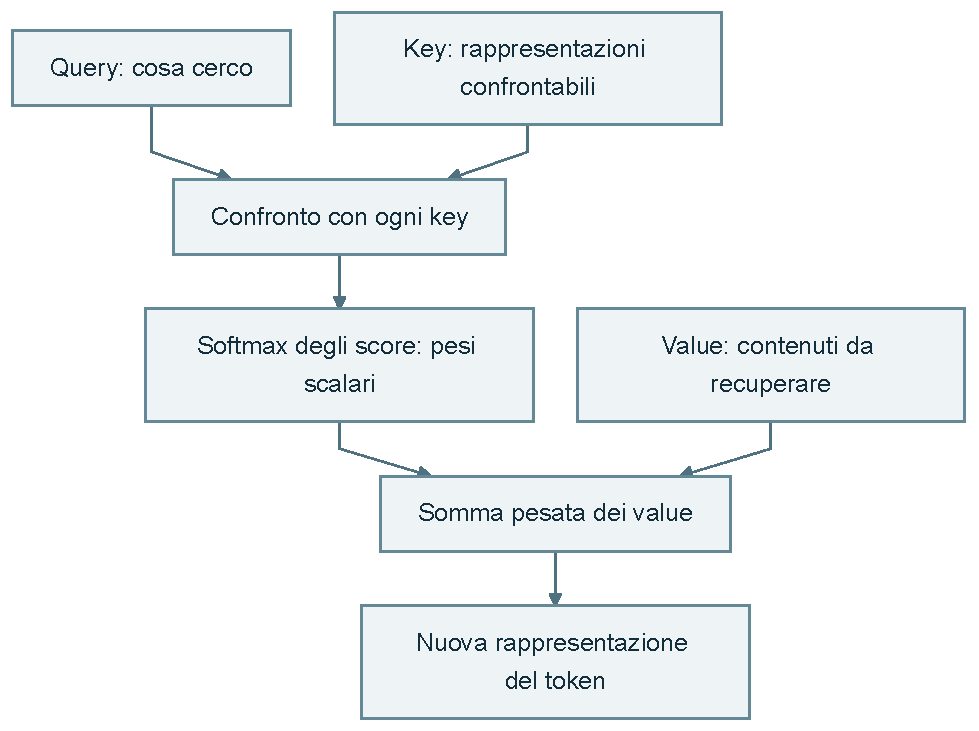
\includegraphics[keepaspectratio]{figure/diagramma_f04_03.pdf}}
% END F04-B0197

% BEGIN F04-B0198
L\textquotesingle analogia riguarda la selezione e la combinazione di contenuti, non dimostra una capacità generale di ragionamento. L\textquotesingle apprendimento sceglie come rappresentare query, key e value affinché l\textquotesingle uscita serva al compito.
% END F04-B0198

% BEGIN F04-B0199
\section{Query, key e value: tre proiezioni dello stesso ingresso (slide 33)}\label{f04-r540}
% END F04-B0199

% BEGIN F04-B0200
Le tre rappresentazioni si ottengono mediante trasformazioni lineari. Con una riga per token:
% END F04-B0200

% BEGIN F04-B0201
\begin{center}
\begin{adjustbox}{max width=\linewidth}
$\displaystyle \boxed{Q=XW^Q,\qquad K=XW^K,\qquad V=XW^V.}$
\end{adjustbox}
\end{center}
% END F04-B0201

% BEGIN F04-B0202
\begin{longtable}[]{@{}lll@{}}
\toprule\noalign{}
Quantità & Forma & Significato \\
\midrule\noalign{}
\endhead
\bottomrule\noalign{}
\endlastfoot
\(X\) & \(T\times D\) & Sequenza di ingresso, con \(D=d_{\mathrm{model}}\) \\
\(W^Q\) & \(D\times d_k\) & Proiezione verso le query \\
\(W^K\) & \(D\times d_k\) & Proiezione verso le key \\
\(W^V\) & \(D\times d_v\) & Proiezione verso i value \\
\(Q,K\) & \(T\times d_k\) & Una query e una key per token \\
\(V\) & \(T\times d_v\) & Un value per token \\
\end{longtable}
% END F04-B0202

% BEGIN F04-B0203
Le slide usano \(d_v=d_k\); la condizione essenziale per il prodotto scalare è che \textbf{query e key abbiano la stessa dimensione}. La dimensione dei value può, in generale, essere distinta. Nell\textquotesingle esempio successivo manteniamo la scelta della slide: \(D=4\) e \(d_k=d_v=3\).
% END F04-B0203

% BEGIN F04-B0204
Il prodotto \(XW^Q\) applica la stessa trasformazione a ogni riga:
% END F04-B0204

% BEGIN F04-B0205
\begin{center}
\begin{adjustbox}{max width=\linewidth}
$\displaystyle 
\begin{aligned}
q_{t,j}&=\sum_{a=1}^{D}X_{t,a}W^Q_{a,j},\\
q_t&=x_tW^Q\in\mathbb R^{1\times d_k}.
\end{aligned}
$
\end{adjustbox}
\end{center}
% END F04-B0205

% BEGIN F04-B0206
Si ripete il procedimento con matrici distinte per \(K\) e \(V\). Proiettare permette di apprendere spazi adatti al confronto e al contenuto da recuperare: l\textquotesingle embedding iniziale non deve già essere la rappresentazione migliore per tutti e tre i ruoli.
% END F04-B0206

% BEGIN F04-B0207
Poiché query, key e value derivano dalla \textbf{stessa sequenza}, si parla di \textbf{self-attention}. Nel richiamo alla cross-attention la query può provenire da una sequenza e key--value da un\textquotesingle altra; non viene sviluppato qui il relativo modulo.
% END F04-B0207

% BEGIN F04-B0208
\begin{figure}[H]
\centering
\pandocbounded{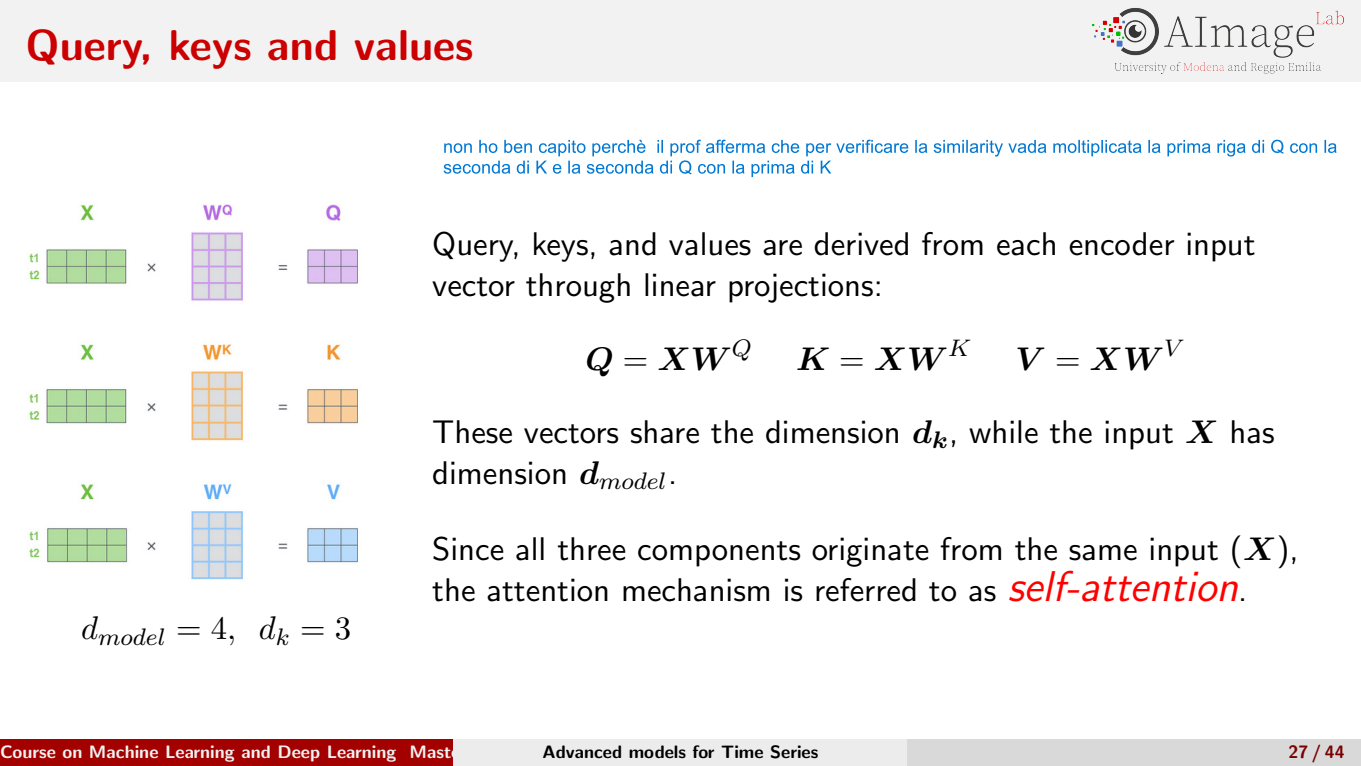
\includegraphics[keepaspectratio]{figure/fig_9a3effeee163c7e6.png}}
\caption{Slide 33 --- Proiezioni e annotazione sul confronto fra righe di Q e K}
\end{figure}
% END F04-B0208

% BEGIN F04-B0209
\subsection{Esempio delle tre proiezioni, con dimensioni esplicite (slide 33)}\label{f04-r572}
% END F04-B0209

% BEGIN F04-B0210
Consideriamo due token di quattro feature:
% END F04-B0210

% BEGIN F04-B0211
\begin{center}
\begin{adjustbox}{max width=\linewidth}
$\displaystyle X=\begin{bmatrix}1&0&1&0\\0&1&0&1\end{bmatrix}.$
\end{adjustbox}
\end{center}
% END F04-B0211

% BEGIN F04-B0212
Le seguenti matrici \(4\times3\) sono un piccolo esempio numerico costruito per esplicitare i prodotti, non valori leggibili nel disegno della slide:
% END F04-B0212

% BEGIN F04-B0213
\begin{center}
\begin{adjustbox}{max width=\linewidth}
$\displaystyle 
W^Q=\begin{bmatrix}1&0&0\\0&1&0\\0&0&0\\0&0&0\end{bmatrix},\quad
W^K=\begin{bmatrix}1&0&1\\2&2&0\\0&0&0\\0&0&0\end{bmatrix},\quad
W^V=\begin{bmatrix}1&2&0\\3&0&1\\0&0&0\\0&0&0\end{bmatrix}.
$
\end{adjustbox}
\end{center}
% END F04-B0213

% BEGIN F04-B0214
La prima riga di \(X\), \((1,0,1,0)\), combina prima e terza riga di ciascuna matrice di proiezione; la seconda combina seconda e quarta. Poiché terza e quarta sono qui nulle:
% END F04-B0214

% BEGIN F04-B0215
\begin{center}
\begin{adjustbox}{max width=\linewidth}
$\displaystyle 
\boxed{Q=\begin{bmatrix}1&0&0\\0&1&0\end{bmatrix},\quad
K=\begin{bmatrix}1&0&1\\2&2&0\end{bmatrix},\quad
V=\begin{bmatrix}1&2&0\\3&0&1\end{bmatrix}.}
$
\end{adjustbox}
\end{center}
% END F04-B0215

% BEGIN F04-B0216
Ogni risultato ha ancora \textbf{due righe}, una per token; la dimensione delle feature è passata da 4 a 3. Il valore \(d_k\) conta le componenti di query e key, non il numero dei token.
% END F04-B0216

% BEGIN F04-B0217
\section{Single-head attention: dal confronto alla somma pesata (slide 34)}\label{f04-r596}
% END F04-B0217

% BEGIN F04-B0218
La \textbf{scaled dot-product attention} esegue in forma matriciale tutti i confronti e tutte le combinazioni:
% END F04-B0218

% BEGIN F04-B0219
\begin{center}
\begin{adjustbox}{max width=\linewidth}
$\displaystyle \boxed{Z=\operatorname{Attention}(Q,K,V)=\operatorname{softmax}_{\mathrm{righe}}\!\left(\frac{QK^T}{\sqrt{d_k}}\right)V.}$
\end{adjustbox}
\end{center}
% END F04-B0219

% BEGIN F04-B0220
La lettura va fatta da dentro verso fuori: prodotti scalari query--key, riscalamento, softmax per riga e prodotto finale con i value.
% END F04-B0220

% BEGIN F04-B0221
\begin{figure}[H]
\centering
\pandocbounded{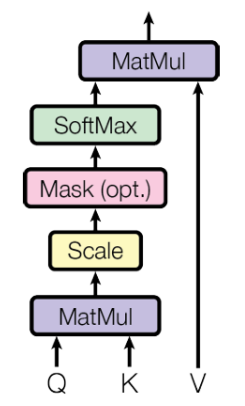
\includegraphics[keepaspectratio]{figure/fig_1a1af14eb3efc6a9.png}}
\caption{Slide 34 --- Flusso dello scaled dot-product attention}
\end{figure}
% END F04-B0221

% BEGIN F04-B0222
\subsection{Perché K viene trasposta e quali righe si confrontano (slide 33--34)}\label{f04-r606}
% END F04-B0222

% BEGIN F04-B0223
\(Q\) e \(K\) hanno forma \(T\times d_k\). Per confrontare ogni riga di \(Q\) con ogni riga di \(K\) occorre il prodotto
% END F04-B0223

% BEGIN F04-B0224
\begin{center}
\begin{adjustbox}{max width=\linewidth}
$\displaystyle \boxed{S_0=QK^T\in\mathbb R^{T\times T},\qquad (S_0)_{t,i}=\sum_{a=1}^{d_k}Q_{t,a}K_{i,a}=q_t\cdot k_i.}$
\end{adjustbox}
\end{center}
% END F04-B0224

% BEGIN F04-B0225
La trasposizione porta le righe delle key sulle colonne della matrice moltiplicata. Per due token si ottiene:
% END F04-B0225

% BEGIN F04-B0226
\begin{center}
\begin{adjustbox}{max width=\linewidth}
$\displaystyle QK^T=\begin{bmatrix}
q_1\cdot k_1&q_1\cdot k_2\\
q_2\cdot k_1&q_2\cdot k_2
\end{bmatrix}.$
\end{adjustbox}
\end{center}
% END F04-B0226

% BEGIN F04-B0227
Questa è la risposta al dubbio annotato nella slide 33: \textbf{non si moltiplicano soltanto la prima riga di \(Q\) con la seconda di \(K\) e la seconda di \(Q\) con la prima di \(K\)}. Quelli sono due confronti incrociati; si calcolano anche i confronti sulla diagonale. Per ogni query si considerano tutte le key ammesse.
% END F04-B0227

% BEGIN F04-B0228
Nel nostro esempio:
% END F04-B0228

% BEGIN F04-B0229
\begin{center}
\begin{adjustbox}{max width=\linewidth}
$\displaystyle 
\begin{aligned}
q_1\cdot k_1&=1\cdot1+0\cdot0+0\cdot1=1,\\
q_1\cdot k_2&=1\cdot2+0\cdot2+0\cdot0=2,\\
q_2\cdot k_1&=0\cdot1+1\cdot0+0\cdot1=0,\\
q_2\cdot k_2&=0\cdot2+1\cdot2+0\cdot0=2,\\
QK^T&=\begin{bmatrix}1&2\\0&2\end{bmatrix}.
\end{aligned}
$
\end{adjustbox}
\end{center}
% END F04-B0229

% BEGIN F04-B0230
Il prodotto è una misura di compatibilità appresa, non necessariamente una correlazione statistica normalizzata. Poiché \(W^Q\) e \(W^K\) sono diversi, \(q_t\) e \(k_t\) non sono in generale lo stesso vettore. Perciò la matrice non deve essere simmetrica e la diagonale \textbf{non deve essere la massima}. Nell\textquotesingle esempio la prima query ha score 2 con la seconda key, maggiore del proprio score diagonale 1. La conservazione dell\textquotesingle ingresso è favorita anche dalla connessione residua esterna, non garantita da una diagonale dominante.
% END F04-B0230

% BEGIN F04-B0231
\subsection{Perché dividere per la radice della dimensione (slide 34)}\label{f04-r635}
% END F04-B0231

% BEGIN F04-B0232
Il prodotto scalare somma \(d_k\) contributi. All\textquotesingle aumentare della dimensione, la sua scala può crescere e produrre score molto separati; la softmax può allora diventare estremamente concentrata, con gradienti piccoli.
% END F04-B0232

% BEGIN F04-B0233
Per chiarire il riscalamento, sotto l\textquotesingle ipotesi illustrativa di componenti indipendenti, a media zero e varianza unitaria, e query e key indipendenti:
% END F04-B0233

% BEGIN F04-B0234
\begin{center}
\begin{adjustbox}{max width=\linewidth}
$\displaystyle 
\begin{aligned}
s&=\sum_{a=1}^{d_k}q_ak_a,\\
\mathbb E[q_ak_a]&=\mathbb E[q_a]\mathbb E[k_a]=0
&&\text{indipendenza e medie nulle},\\
\operatorname{var}(q_ak_a)&=\mathbb E[q_a^2]\mathbb E[k_a^2]=1
&&\text{indipendenza e secondi momenti unitari},\\
\operatorname{var}(s)&=\sum_a1=d_k
&&\text{somma di contributi indipendenti},\\
\operatorname{var}\!\left(\frac{s}{\sqrt{d_k}}\right)&=\frac{d_k}{d_k}=1
&&\text{varianza di una quantità riscalata}.
\end{aligned}
$
\end{adjustbox}
\end{center}
% END F04-B0234

% BEGIN F04-B0235
Non è una garanzia che query e key apprese soddisfino queste ipotesi; è la motivazione di scala. Per \(d_k=64\), il denominatore è \textbf{8}, non 64. La normalizzazione degli score e la LayerNorm hanno posizioni e scopi collegati alla stabilità, ma sono operazioni diverse.
% END F04-B0235

% BEGIN F04-B0236
\begin{quote}
\textbf{Precisazione slide 34 --- Matrici e fattore di scala}
\end{quote}
% END F04-B0236

% BEGIN F04-B0237
\begin{quote}
Nella formula, \(Q,K,V\) sono matrici che raccolgono vettori per token, non tre singoli vettori di lunghezza 64. \(d_k=64\) è un esempio di dimensione delle query e delle key; il fattore di scala è \(1/\sqrt{d_k}\). Il numero di righe resta il numero di token e non viene sostituito da \(d_k\).
\end{quote}
% END F04-B0237

% BEGIN F04-B0238
\subsection{Softmax per riga: esempio completo (slide 34)}\label{f04-r660}
% END F04-B0238

% BEGIN F04-B0239
Con \(d_k=3\), si riscalano gli score:
% END F04-B0239

% BEGIN F04-B0240
\begin{center}
\begin{adjustbox}{max width=\linewidth}
$\displaystyle S=\frac1{\sqrt3}\begin{bmatrix}1&2\\0&2\end{bmatrix}
\approx\begin{bmatrix}0.577350&1.154701\\0&1.154701\end{bmatrix}.$
\end{adjustbox}
\end{center}
% END F04-B0240

% BEGIN F04-B0241
Per la prima riga:
% END F04-B0241

% BEGIN F04-B0242
\begin{center}
\begin{adjustbox}{max width=\linewidth}
$\displaystyle 
\begin{aligned}
\alpha_{1,1}
&=\frac{e^{1/\sqrt3}}{e^{1/\sqrt3}+e^{2/\sqrt3}}
=\frac1{1+e^{1/\sqrt3}}\approx0.359543,\\
\alpha_{1,2}&=1-\alpha_{1,1}\approx0.640457.
\end{aligned}
$
\end{adjustbox}
\end{center}
% END F04-B0242

% BEGIN F04-B0243
Si ripete sulla seconda riga, separatamente:
% END F04-B0243

% BEGIN F04-B0244
\begin{center}
\begin{adjustbox}{max width=\linewidth}
$\displaystyle 
\begin{aligned}
\alpha_{2,1}&=\frac1{1+e^{2/\sqrt3}}\approx0.239632,\\
\alpha_{2,2}&=1-\alpha_{2,1}\approx0.760368.
\end{aligned}
$
\end{adjustbox}
\end{center}
% END F04-B0244

% BEGIN F04-B0245
La matrice dei coefficienti è quindi
% END F04-B0245

% BEGIN F04-B0246
\begin{center}
\begin{adjustbox}{max width=\linewidth}
$\displaystyle \boxed{A\approx\begin{bmatrix}0.359543&0.640457\\0.239632&0.760368\end{bmatrix}.}$
\end{adjustbox}
\end{center}
% END F04-B0246

% BEGIN F04-B0247
Ogni riga somma a 1; le colonne non devono farlo. La prima riga risponde alla domanda «quanto pesa ciascun value per costruire l\textquotesingle uscita della prima query?». La seconda risponde alla stessa domanda per la seconda query. Applicare la softmax per colonne normalizzerebbe una domanda diversa e non realizzerebbe la formula descritta.
% END F04-B0247

% BEGIN F04-B0248
\subsection{Il prodotto finale con V ricostruisce i token (slide 34)}\label{f04-r693}
% END F04-B0248

% BEGIN F04-B0249
Il prodotto
% END F04-B0249

% BEGIN F04-B0250
\begin{center}
\begin{adjustbox}{max width=\linewidth}
$\displaystyle \boxed{Z=AV\in\mathbb R^{T\times d_v},\qquad z_t=\sum_{i=1}^{T}A_{t,i}v_i}$
\end{adjustbox}
\end{center}
% END F04-B0250

% BEGIN F04-B0251
usa i pesi per combinare i value. Con \(V=\begin{bmatrix}1&2&0\\3&0&1\end{bmatrix}\):
% END F04-B0251

% BEGIN F04-B0252
\begin{center}
\begin{adjustbox}{max width=\linewidth}
$\displaystyle 
\begin{aligned}
z_1&\approx0.359543(1,2,0)+0.640457(3,0,1)\\
&\approx(0.359543+1.921372,\;0.719085,\;0.640457)\\
&\approx(2.280915,0.719085,0.640457),\\
z_2&\approx0.239632(1,2,0)+0.760368(3,0,1)\\
&\approx(0.239632+2.281105,\;0.479263,\;0.760368)\\
&\approx(2.520737,0.479263,0.760368).
\end{aligned}
$
\end{adjustbox}
\end{center}
% END F04-B0252

% BEGIN F04-B0253
I conti usano i coefficienti non arrotondati fino al risultato finale. Si ottiene ancora una sequenza di due elementi, ora con tre feature ciascuno. Ogni uscita combina entrambe le righe di \(V\), con pesi diversi.
% END F04-B0253

% BEGIN F04-B0254
Il passaggio \(AV\) è lineare rispetto a \(V\) \textbf{a coefficienti fissati}. L\textquotesingle intero meccanismo è però non lineare rispetto all\textquotesingle ingresso, perché anche \(A\) dipende da \(X\) attraverso proiezioni, prodotti e softmax. Non è quindi uno strato lineare con una matrice di pesi costante per tutte le sequenze.
% END F04-B0254

% BEGIN F04-B0255
\section{Multi-Head Attention: più confronti in parallelo (slide 35--36)}\label{f04-r716}
% END F04-B0255

% BEGIN F04-B0256
Una sola testa costruisce un insieme di relazioni mediante le sue proiezioni. La \textbf{Multi-Head Attention}, o \textbf{MHA}, ripete il procedimento con proiezioni distinte, così che rappresentazioni differenti possano concorrere alla stessa uscita.
% END F04-B0256

% BEGIN F04-B0257
Per \(H\) teste:
% END F04-B0257

% BEGIN F04-B0258
\begin{center}
\begin{adjustbox}{max width=\linewidth}
$\displaystyle \boxed{\begin{aligned}
Z_h&=\operatorname{Attention}(XW_h^Q,XW_h^K,XW_h^V),\qquad h=1,\ldots,H,\\
\operatorname{MHA}(X)&=\operatorname{Concat}_{\mathrm{feature}}(Z_1,\ldots,Z_H)W^O.
\end{aligned}}$
\end{adjustbox}
\end{center}
% END F04-B0258

% BEGIN F04-B0259
La concatenazione avviene sulle \textbf{feature dello stesso token}, non sull\textquotesingle asse della sequenza. Se ogni \(Z_h\) ha forma \(T\times d_v\), la concatenazione ha forma \(T\times Hd_v\) e
% END F04-B0259

% BEGIN F04-B0260
\begin{center}
\begin{adjustbox}{max width=\linewidth}
$\displaystyle \boxed{W^O\in\mathbb R^{Hd_v\times D},\qquad\operatorname{MHA}(X)\in\mathbb R^{T\times D}.}$
\end{adjustbox}
\end{center}
% END F04-B0260

% BEGIN F04-B0261
Prima si tengono le uscite delle teste affiancate, poi si apprende come combinarle con la proiezione \(W^O\). Si torna così alla dimensione richiesta dalla somma residua.
% END F04-B0261

% BEGIN F04-B0262
\begin{figure}[H]
\centering
\pandocbounded{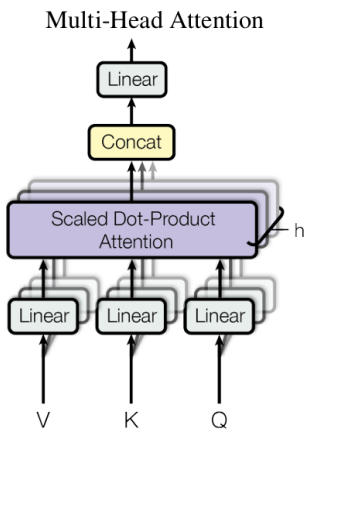
\includegraphics[keepaspectratio]{figure/fig_852979b0e322a93f.png}}
\caption{Slide 35 --- Struttura della multi-head attention}
\end{figure}
% END F04-B0262

% BEGIN F04-B0263
\begin{figure}[H]
\centering
\pandocbounded{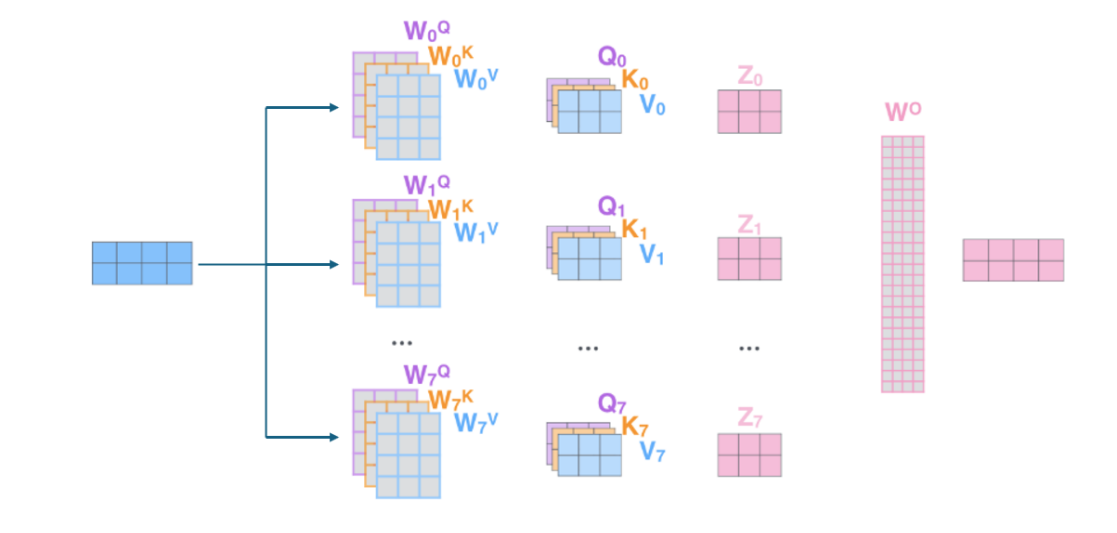
\includegraphics[keepaspectratio]{figure/fig_1a88427c5d5e67b5.png}}
\caption{Slide 36 --- Proiezioni distinte, teste e ricombinazione delle feature}
\end{figure}
% END F04-B0263

% BEGIN F04-B0264
\subsection{Esempio di concatenazione e proiezione (slide 35--36)}\label{f04-r737}
% END F04-B0264

% BEGIN F04-B0265
Con \(T=2\), \(H=2\) e \(d_v=1\), supponiamo che due teste abbiano prodotto:
% END F04-B0265

% BEGIN F04-B0266
\begin{center}
\begin{adjustbox}{max width=\linewidth}
$\displaystyle Z_1=\begin{bmatrix}1\\2\end{bmatrix},\qquad
Z_2=\begin{bmatrix}3\\4\end{bmatrix}.$
\end{adjustbox}
\end{center}
% END F04-B0266

% BEGIN F04-B0267
La concatenazione per feature è
% END F04-B0267

% BEGIN F04-B0268
\begin{center}
\begin{adjustbox}{max width=\linewidth}
$\displaystyle C=\begin{bmatrix}1&3\\2&4\end{bmatrix},$
\end{adjustbox}
\end{center}
% END F04-B0268

% BEGIN F04-B0269
non una sequenza di quattro righe. Se \(D=2\) e
% END F04-B0269

% BEGIN F04-B0270
\begin{center}
\begin{adjustbox}{max width=\linewidth}
$\displaystyle W^O=\begin{bmatrix}1&1\\1&-1\end{bmatrix},$
\end{adjustbox}
\end{center}
% END F04-B0270

% BEGIN F04-B0271
allora
% END F04-B0271

% BEGIN F04-B0272
\begin{center}
\begin{adjustbox}{max width=\linewidth}
$\displaystyle CW^O=\begin{bmatrix}1+3&1-3\\2+4&2-4\end{bmatrix}
=\boxed{\begin{bmatrix}4&-2\\6&-2\end{bmatrix}}.$
\end{adjustbox}
\end{center}
% END F04-B0272

% BEGIN F04-B0273
Rimangono due token e la proiezione combina le due informazioni di testa per ciascuno. È l\textquotesingle analogia con più filtri convoluzionali: si apprendono più trasformazioni parallele, senza assegnare manualmente a ogni testa un significato prestabilito.
% END F04-B0273

% BEGIN F04-B0274
Somma o media delle teste sarebbero altre regole di aggregazione, ma la formula della MHA qui studiata usa \textbf{concatenazione seguita da proiezione}. Nella configurazione frequente \(D=Hd_k\) e \(d_v=d_k\), il totale delle feature concatenate è già \(D\), ma \(W^O\) rimane una trasformazione apprendibile.
% END F04-B0274

% BEGIN F04-B0275
\begin{quote}
\textbf{Precisazione slide 35--36 --- Le teste non moltiplicano la lunghezza}
\end{quote}
% END F04-B0275

% BEGIN F04-B0276
\begin{quote}
Ogni testa produce \(T\) righe; le \(H\) sequenze sono risultati intermedi paralleli. La concatenazione finale della MHA unisce le feature allineate alla stessa posizione, dando \(T\times Hd_v\), non \(HT\) token successivamente compressi lungo il tempo. Una proiezione lineare applicata per token cambia le feature, non il numero dei token.
\end{quote}
% END F04-B0276

% BEGIN F04-B0277
All\textquotesingle interno dell\textquotesingle attention le teste possono cambiare dimensione delle feature; il modulo completo deve restituire \(D\) per la somma residua. Quando si dice che il blocco conserva la forma, si parla della sua interfaccia, non dell\textquotesingle assenza di proiezioni interne.
% END F04-B0277

% BEGIN F04-B0278
\section{Dalla sequenza di rappresentazioni alla classificazione (slide 37--38)}\label{f04-r766}
% END F04-B0278

% BEGIN F04-B0279
Dopo una pila di encoder rimane una matrice \(Z\in\mathbb R^{T\times D}\), non un unico vettore globale. Ogni riga è una rappresentazione \textbf{contestualizzata} della posizione: può aver ricevuto informazioni dagli altri token, ma rimane una riga della sequenza.
% END F04-B0279

% BEGIN F04-B0280
Per classificare l\textquotesingle intera frase o serie si può costruire un vettore globale mediante \textbf{average pooling} oppure tramite un \textbf{token di classificazione}. È l\textquotesingle interfaccia fra estrattore e classificatore, analoga a quella discussa per le CNN in \hyperref[fonte02]{reti convoluzionali}.
% END F04-B0280

% BEGIN F04-B0281
\subsection{Average pooling sui token (slide 37)}\label{f04-r772}
% END F04-B0281

% BEGIN F04-B0282
La media viene calcolata lungo l\textquotesingle asse della sequenza, separatamente per ogni feature:
% END F04-B0282

% BEGIN F04-B0283
\begin{center}
\begin{adjustbox}{max width=\linewidth}
$\displaystyle \boxed{g=\frac1T\sum_{t=1}^{T}z_t\in\mathbb R^{1\times D},\qquad
g_j=\frac1T\sum_{t=1}^{T}Z_{t,j}.}$
\end{adjustbox}
\end{center}
% END F04-B0283

% BEGIN F04-B0284
Si sommano le righe e si divide per il loro numero. Non si fa la media di tutte le feature in un singolo scalare. Per esempio:
% END F04-B0284

% BEGIN F04-B0285
\begin{center}
\begin{adjustbox}{max width=\linewidth}
$\displaystyle Z=\begin{bmatrix}1&3\\3&1\end{bmatrix}
\quad\Longrightarrow\quad
g=\left(\frac{1+3}2,\frac{3+1}2\right)=(2,2).$
\end{adjustbox}
\end{center}
% END F04-B0285

% BEGIN F04-B0286
Una testa lineare per \(C\) classi produce
% END F04-B0286

% BEGIN F04-B0287
\begin{center}
\begin{adjustbox}{max width=\linewidth}
$\displaystyle \boxed{s=gW_c+b_c\in\mathbb R^{1\times C},\qquad W_c\in\mathbb R^{D\times C},\quad b_c\in\mathbb R^{1\times C}.}$
\end{adjustbox}
\end{center}
% END F04-B0287

% BEGIN F04-B0288
Con \(C=3\), \(W_c=\begin{bmatrix}1&0&-1\\0&0.5&1\end{bmatrix}\) e bias nullo:
% END F04-B0288

% BEGIN F04-B0289
\begin{center}
\begin{adjustbox}{max width=\linewidth}
$\displaystyle s=(2,2)W_c=(2,1,0).$
\end{adjustbox}
\end{center}
% END F04-B0289

% BEGIN F04-B0290
Sono tre score di classe. La softmax darebbe circa \((0.66524,0.24473,0.09003)\), mentre una loss di classificazione può lavorare direttamente sugli score secondo la propria definizione, come spiegato in \hyperref[fonte01]{Multilayer Perceptron}. I parametri della testa sono \(DC+C=C(D+1)\): qui \(3(2+1)=9\) con bias incluso, indipendentemente da \(T\).
% END F04-B0290

% BEGIN F04-B0291
Il pooling finale riduce la sequenza; non contraddice il fatto che i singoli blocchi encoder conservino la lunghezza. Somma e media sono operazioni distinte: la media richiede il divisore \(T\), importante quando si confrontano lunghezze diverse.
% END F04-B0291

% BEGIN F04-B0292
\subsection{Token {[}CLS{]}: una posizione dedicata al riassunto (slide 38)}\label{f04-r797}
% END F04-B0292

% BEGIN F04-B0293
In alternativa si antepone un token speciale all\textquotesingle ingresso. Se gli elementi originari sono \(T\), la sequenza elaborata ha forma \((T+1)\times D\). Il token partecipa all\textquotesingle attention; alla fine si preleva la sua rappresentazione:
% END F04-B0293

% BEGIN F04-B0294
\begin{center}
\begin{adjustbox}{max width=\linewidth}
$\displaystyle \boxed{g=z_{\mathrm{[CLS]}}\in\mathbb R^{1\times D}.}$
\end{adjustbox}
\end{center}
% END F04-B0294

% BEGIN F04-B0295
Per esempio, tre token ordinari più {[}CLS{]} danno quattro righe; dopo i blocchi rimangono quattro righe e soltanto quella corrispondente a {[}CLS{]} viene data alla testa di classificazione. Il token speciale non è di per sé l\textquotesingle etichetta della classe: è una posizione a cui il modello può imparare a trasferire informazioni utili.
% END F04-B0295

% BEGIN F04-B0296
La selezione finale della riga non è una somma manuale: il riassunto è stato costruito dalle interazioni nei blocchi. Il modello deve essere addestrato o adattato a utilizzare quella posizione; inserire un token arbitrario in una rete preaddestrata non garantisce che il relativo vettore sia già un buon riassunto.
% END F04-B0296

% BEGIN F04-B0297
\pandocbounded{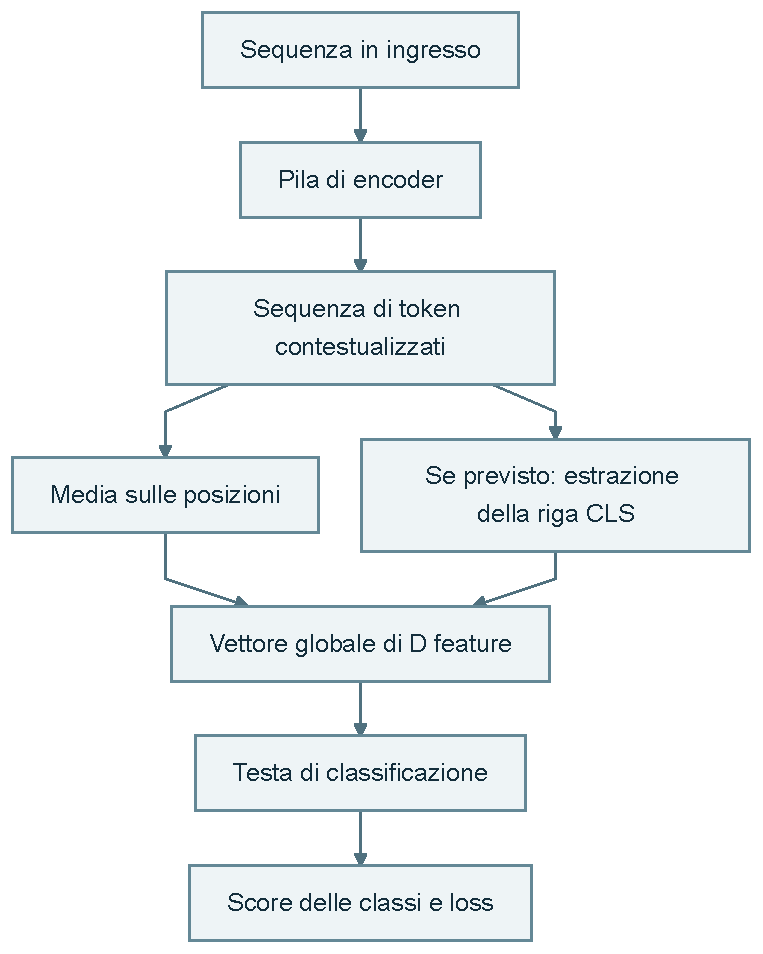
\includegraphics[keepaspectratio]{figure/diagramma_f04_04.pdf}}
% END F04-B0297

% BEGIN F04-B0298
Il pooling medio può essere calcolato su rappresentazioni già disponibili, ma la sua efficacia va valutata rispetto al compito e all\textquotesingle addestramento del modello. Non è intercambiabile per definizione con una rappresentazione {[}CLS{]} appresa.
% END F04-B0298

% BEGIN F04-B0299
\section{TCN e Transformer: confronto, modalità e costi (slide 39--41)}\label{f04-r821}
% END F04-B0299

% BEGIN F04-B0300
Le due famiglie organizzano in modo diverso il contesto disponibile:
% END F04-B0300

% BEGIN F04-B0301
\begin{longtable}[]{@{}
  >{\raggedright\arraybackslash}p{(\linewidth - 4\tabcolsep) * \real{0.3333}}
  >{\raggedright\arraybackslash}p{(\linewidth - 4\tabcolsep) * \real{0.3333}}
  >{\raggedright\arraybackslash}p{(\linewidth - 4\tabcolsep) * \real{0.3333}}@{}}
\toprule\noalign{}
\begin{minipage}[b]{\linewidth}\raggedright
Aspetto
\end{minipage} & \begin{minipage}[b]{\linewidth}\raggedright
TCN descritta
\end{minipage} & \begin{minipage}[b]{\linewidth}\raggedright
Transformer encoder descritto
\end{minipage} \\
\midrule\noalign{}
\endhead
\bottomrule\noalign{}
\endlastfoot
Interazioni & Filtri causali locali con dilatazioni fissate & Coefficienti query--key calcolati dal contenuto \\
Contesto di un\textquotesingle uscita & Campo recettivo determinato da kernel, dilatazioni e profondità & Tutti i token ammessi dall\textquotesingle attention \\
Asse temporale & Mappe indicizzate per posizione & Token indicizzati per posizione \\
Parallelismo & Posizioni e filtri nello stesso livello & Proiezioni, teste, confronti e MLP per token \\
Trasformazioni & Convoluzioni e blocchi residui & MHA, MLP, residui e LayerNorm \\
Memoria & Attivazioni delle mappe convoluzionali & Attivazioni dei token e, nell\textquotesingle implementazione diretta, matrici di attention \\
\end{longtable}
% END F04-B0301

% BEGIN F04-B0302
«Campo recettivo non fisso» nei Transformer indica che cambiano \textbf{le rilevanze attribuite alle posizioni}. Nell\textquotesingle encoder con attention piena le posizioni potenzialmente accessibili sono già tutte quelle del contesto fornito. Non vengono creati accessi a una sequenza infinita o a informazioni non presenti nell\textquotesingle ingresso.
% END F04-B0302

% BEGIN F04-B0303
Il vincolo causale non nasce dal semplice uso della parola Transformer: l\textquotesingle encoder qui studiato può usare entrambi i lati della sequenza. Se il compito richiede predizioni online, bisogna impedire l\textquotesingle accesso al futuro mediante una configurazione appropriata. I dettagli del masking restano fuori dal perimetro sviluppato.
% END F04-B0303

% BEGIN F04-B0304
\subsection{Stesso meccanismo, ingressi di modalità diverse (slide 39--41)}\label{f04-r838}
% END F04-B0304

% BEGIN F04-B0305
L\textquotesingle attention opera su vettori. Se testo, musica, misure numeriche o porzioni di immagini vengono rappresentati in uno spazio di feature compatibile, lo stesso tipo di blocco può elaborarli.
% END F04-B0305

% BEGIN F04-B0306
Per un\textquotesingle immagine, l\textquotesingle intuizione è dividerla in piccoli quadrati, rappresentare ciascuna \textbf{patch} con un vettore e organizzare i vettori in una sequenza. L\textquotesingle attention può allora collegare parti diverse dell\textquotesingle immagine. È il richiamo ai Vision Transformer, senza sviluppare un\textquotesingle architettura visiva completa.
% END F04-B0306

% BEGIN F04-B0307
L\textquotesingle analogia delle patch come «parole visive» riguarda il formato a token. Non significa che un tokenizer testuale possa elaborare direttamente pixel grezzi o che basti rendere uguali le dimensioni per ottenere comprensione fra modalità. Servono proiezioni compatibili e un addestramento che dia significato alle relazioni. L\textquotesingle architettura comune rende possibile la fusione, non la realizza automaticamente.
% END F04-B0307

% BEGIN F04-B0308
\subsection{Dove sono i parametri: proiezioni e MLP (slide 39--41)}\label{f04-r846}
% END F04-B0308

% BEGIN F04-B0309
MHA richiede proiezioni per query, key e value di ogni testa, oltre alla proiezione di uscita. L\textquotesingle MLP aggiunge due matrici, e ogni blocco della pila ha i propri pesi. La condivisione del MLP fra posizioni non implica condivisione fra tutti i blocchi.
% END F04-B0309

% BEGIN F04-B0310
Con \(H\) teste, dimensioni \(d_k=d_v\) e bias omessi:
% END F04-B0310

% BEGIN F04-B0311
\begin{center}
\begin{adjustbox}{max width=\linewidth}
$\displaystyle 
\begin{aligned}
P_Q+P_K+P_V&=3HDd_k &&\text{tre proiezioni per testa},\\
P_O&=Hd_kD &&\text{ricombinazione delle feature},\\
\boxed{P_{\mathrm{MHA}}}&=\boxed{4HDd_k.}
\end{aligned}
$
\end{adjustbox}
\end{center}
% END F04-B0311

% BEGIN F04-B0312
Se si mantiene \(D=Hd_k\), il conteggio diventa \(4D^2\). A \(D\) fisso, aumentare \(H\) riducendo \(d_k\) proporzionalmente non moltiplica automaticamente i pesi della MHA. Se invece si mantiene \(d_k\) fisso e si aumentano le teste, il conteggio cresce con \(H\). Occorre sempre dichiarare quale dimensione è mantenuta costante.
% END F04-B0312

% BEGIN F04-B0313
Per il feed-forward con dimensione interna \(F\):
% END F04-B0313

% BEGIN F04-B0314
\begin{center}
\begin{adjustbox}{max width=\linewidth}
$\displaystyle 
\begin{aligned}
P_{W_1}&=DF,\qquad P_{W_2}=FD,\\
\boxed{P_{\mathrm{FFN}}}&=\boxed{2DF}\quad\text{senza bias},\\
P_{\mathrm{FFN,con\ bias}}&=2DF+F+D.
\end{aligned}
$
\end{adjustbox}
\end{center}
% END F04-B0314

% BEGIN F04-B0315
Con \(D=4,H=2,d_k=2,F=8\), la MHA ha \(4\cdot2\cdot4\cdot2=64\) pesi e il feed-forward \(2\cdot4\cdot8=64\) pesi; includendo i bias del solo FFN, quest\textquotesingle ultimo arriva a 76. Sono conteggi delle trasformazioni, non di tutto il modello con embedding e testa finale.
% END F04-B0315

% BEGIN F04-B0316
Per una configurazione illustrativa più grande, \(D=512\) e \(F=4D=2048\), si hanno \(1\,048\,576\) pesi di MHA e \(2\,097\,152\) pesi di FFN. Fra queste due componenti il FFN pesa \(2/3\), circa il 66.7\%. Può essere la parte predominante, ma una quota dell\textquotesingle80\% non è una proprietà universale: dipende dalle dimensioni interne e da quali componenti si includono nel totale. La stessa cautela nel distinguere estrattore e parte densa era necessaria per VGG in \hyperref[fonte02]{reti convoluzionali}.
% END F04-B0316

% BEGIN F04-B0317
Il numero dei parametri dei blocchi descritti non cresce direttamente con \(T\): le proiezioni e il MLP vengono riutilizzati sulle posizioni. Ciò che cresce con \(T\) è il \textbf{calcolo e la memoria delle attivazioni}.
% END F04-B0317

% BEGIN F04-B0318
\subsection{Lunghezza del contesto e matrici di attention (slide 39--41)}\label{f04-r878}
% END F04-B0318

% BEGIN F04-B0319
Una sequenza più lunga richiede più righe di rappresentazioni in ogni blocco. Per una testa con attention piena, inoltre, \(QK^T\) ha \(T^2\) coefficienti:
% END F04-B0319

% BEGIN F04-B0320
\begin{center}
\begin{adjustbox}{max width=\linewidth}
$\displaystyle \boxed{QK^T\in\mathbb R^{T\times T}\quad\Longrightarrow\quad T^2\text{ score per testa}.}$
\end{adjustbox}
\end{center}
% END F04-B0320

% BEGIN F04-B0321
Con 100 token sono 10 000 score; con 200 token sono 40 000. Raddoppiare la lunghezza quadruplica i confronti della matrice piena. Con otto teste, nell\textquotesingle implementazione diretta si avrebbero rispettivamente 80 000 e 320 000 score, prima di considerare batch e numero di blocchi.
% END F04-B0321

% BEGIN F04-B0322
Questa crescita si aggiunge ai vettori di feature, alle attivazioni dei MLP e allo stato necessario al training. Non significa che ogni implementazione debba materializzare sempre tutte le matrici allo stesso modo; chiarisce il costo della formula diretta studiata.
% END F04-B0322

% BEGIN F04-B0323
L\textquotesingle esempio di un libro molto lungo rende intuitiva la differenza rispetto a comprimere tutto in un singolo stato ricorrente: preservare una rappresentazione per ogni elemento è costoso. Parole e token non coincidono necessariamente, e ogni modello concreto ha limiti di contesto e memoria: non si assume che una sequenza arbitrariamente lunga entri interamente nel modello.
% END F04-B0323

% BEGIN F04-B0324
\subsection{Cenno conclusivo: cache di key e value nella generazione (slide 39--41, estensione orale)}\label{f04-r890}
% END F04-B0324

% BEGIN F04-B0325
Nella generazione progressiva, una procedura ingenua potrebbe ricalcolare a ogni nuovo token tutte le rappresentazioni del prefisso precedente. Questo ripeterebbe molto lavoro. La \textbf{KV cache} conserva le key e i value già calcolati, per riutilizzarli quando arriva il nuovo elemento.
% END F04-B0325

% BEGIN F04-B0326
Per il singolo livello e la singola testa, se il prefisso contiene \(T\) elementi, la cache contiene \(T\) righe di key e \(T\) righe di value. Dopo un nuovo elemento le righe diventano \(T+1\): si aggiungono le sue rappresentazioni e la nuova query può confrontarsi con le key conservate. Il nuovo token deve comunque interagire con il contesto: la cache riduce ricalcoli, non rende nullo il costo dell\textquotesingle attention e occupa memoria crescente.
% END F04-B0326

% BEGIN F04-B0327
Il riuso così descritto riguarda una generazione \textbf{causale}: aggiungere un token futuro non deve cambiare le rappresentazioni già calcolate del passato. Non si trasferisce automaticamente all\textquotesingle encoder bidirezionale pieno qui studiato, dove un token precedente potrebbe cambiare rappresentazione vedendo il nuovo elemento. La cache viene mantenuta nei livelli e nelle teste interessate, non è soltanto una lista di token grezzi. I dettagli implementativi non sono sviluppati.
% END F04-B0327

% BEGIN F04-B0328
\section{Confine della spiegazione e materiale rinviato (slide 42--60)}\label{f04-r898}
% END F04-B0328

% BEGIN F04-B0329
La spiegazione si conclude dopo il confronto delle architetture e il cenno alla KV cache. L\textquotesingle ultima slide di contenuto corrispondente è il riepilogo stampato \textbf{32/44}, completato alla \textbf{pagina PDF 41}. La pagina PDF 42 apre invece «Loss Function for Regression», numerata 33/44.
% END F04-B0329

% BEGIN F04-B0330
\begin{quote}
\textbf{Slide 42--60 --- Materiale nel PDF non ancora spiegato}
\end{quote}
% END F04-B0330

% BEGIN F04-B0331
\begin{quote}
La parte successiva contiene loss di regressione, MSE e MAE, discretizzazione del target in intervalli, limiti delle penalizzazioni simmetriche, quantili e quantile loss. La trascrizione rinvia esplicitamente questi argomenti alla spiegazione successiva. Non vengono integrati come contenuti già trattati, né si aggiungono qui derivazioni o esempi di queste loss. Le pagine 61--63 contengono riferimenti e ringraziamenti.
\end{quote}
% END F04-B0331

% BEGIN F04-B0332
La causalità delle TCN, il riassunto delle RNN e la differenza fra parametri e attivazioni si collegano a \hyperref[fonte03]{reti ricorrenti}; filtri, canali, campo recettivo, pooling, residui e BatchNorm a \hyperref[fonte02]{reti convoluzionali}; MLP, ReLU, softmax e loss di classificazione a \hyperref[fonte01]{Multilayer Perceptron}.
% END F04-B0332

% BEGIN F04-B0333
\section{Riepilogo delle forme e delle formule (slide 5--41)}\label{f04-r907}
% END F04-B0333

% BEGIN F04-B0334
\begin{longtable}[]{@{}
  >{\raggedright\arraybackslash}p{(\linewidth - 4\tabcolsep) * \real{0.3333}}
  >{\raggedright\arraybackslash}p{(\linewidth - 4\tabcolsep) * \real{0.3333}}
  >{\raggedright\arraybackslash}p{(\linewidth - 4\tabcolsep) * \real{0.3333}}@{}}
\toprule\noalign{}
\begin{minipage}[b]{\linewidth}\raggedright
Operazione
\end{minipage} & \begin{minipage}[b]{\linewidth}\raggedright
Formula o forma
\end{minipage} & \begin{minipage}[b]{\linewidth}\raggedright
Da ricordare
\end{minipage} \\
\midrule\noalign{}
\endhead
\bottomrule\noalign{}
\endlastfoot
Conv1D multicanale & \(Y_{t,o}=b_o+\sum_{i,c}X_{t+i,c}K_{i,c,o}\) & Filtro condiviso lungo un solo asse \\
Parametri Conv1D & \(C_{\mathrm{out}}(kC_{\mathrm{in}}+1)\) & Con bias; non dipendono da \(T\) \\
Dilatazione causale & \(y_t=\sum_{i=0}^{k-1}x_{t-di}\omega_i\) & Punti distanziati di \(d\) \\
Ampiezza del kernel dilatato & \(1+(k-1)d\) & Ampiezza coperta, non numero di pesi \\
Padding causale & \(P_{\mathrm{sinistra}}=(k-1)d\) & Stride 1, stessa lunghezza in uscita \\
Campo recettivo & \(r_\ell=r_{\ell-1}+(k_\ell-1)d_\ell j_{\ell-1}\) & \(j_\ell=s_\ell j_{\ell-1}\) \\
Sequenza Transformer & \(X:T\times D\) & Una riga per token \\
Feed-forward & \(\operatorname{ReLU}(y_tW_1+b_1)W_2+b_2\) & Stessi pesi sulle posizioni; \(D\to F\to D\) \\
LayerNorm & \(y_j=\gamma_j(x_j-\mu)/\sqrt{v+\epsilon}+\beta_j\) & Statistiche sulle feature del singolo token \\
Proiezioni & \(Q=XW^Q\), \(K=XW^K\), \(V=XW^V\) & Q e K: \(T\times d_k\); V: \(T\times d_v\) \\
Score & \(QK^T:T\times T\) & Riga = query; colonna = key \\
Scala & \(S=QK^T/\sqrt{d_k}\) & Con \(d_k=64\) si divide per 8 \\
Pesi & \(A=\operatorname{softmax}_{\mathrm{righe}}(S)\) & Ogni riga somma a 1 \\
Attention & \(Z=AV:T\times d_v\) & Somma pesata dei value per query \\
Multi-head & \(\operatorname{Concat}(Z_1,\ldots,Z_H)W^O\) & Concatenazione sulle feature, uscita \(T\times D\) \\
Residui e norm & \(Y=\operatorname{LN}_1(X+\operatorname{MHA}(X))\); \(B=\operatorname{LN}_2(Y+\operatorname{FFN}(Y))\) & Forma del blocco conservata \\
Average pooling & \(g=T^{-1}\sum_tz_t\) & Da \(T\times D\) a un vettore di \(D\) feature \\
Token {[}CLS{]} & Ingresso \((T+1)\times D\), poi estrazione di una riga & Il riassunto va appreso dal modello \\
\end{longtable}
% END F04-B0334

% BEGIN F04-B0335
\begin{quote}
\textbf{Percorso essenziale da saper ricostruire}
\end{quote}
% END F04-B0335

% BEGIN F04-B0336
\begin{quote}
Le TCN combinano localmente una sequenza usando filtri condivisi, dilatati e causali. Il Transformer rende invece dinamici i coefficienti delle interazioni: proietta i token in query, key e value; confronta ogni query con le key; normalizza gli score per riga; combina i value. Più teste offrono proiezioni diverse, poi ricombinate sulle feature. Residui, LayerNorm e MLP completano il blocco, mantenendone la forma. Per classificare l\textquotesingle intera sequenza occorre infine un riassunto, per esempio media dei token o rappresentazione {[}CLS{]}.
\end{quote}
% END F04-B0336

% BEGIN F04-B0337
\section{Errata e precisazioni principali (slide 5--41)}\label{f04-r933}
% END F04-B0337

% BEGIN F04-B0338
\begin{longtable}[]{@{}
  >{\raggedright\arraybackslash}p{(\linewidth - 2\tabcolsep) * \real{0.5000}}
  >{\raggedright\arraybackslash}p{(\linewidth - 2\tabcolsep) * \real{0.5000}}@{}}
\toprule\noalign{}
\begin{minipage}[b]{\linewidth}\raggedright
Riferimento
\end{minipage} & \begin{minipage}[b]{\linewidth}\raggedright
Precisazione
\end{minipage} \\
\midrule\noalign{}
\endhead
\bottomrule\noalign{}
\endlastfoot
Slide 5--6 & LeNet-5 non è la prima comparsa assoluta delle idee convoluzionali. 1D descrive l\textquotesingle asse di scorrimento, non l\textquotesingle assenza di canali. \\
Slide 7--8 & La formula a ritardi e l\textquotesingle esempio a finestre usano convenzioni di orientamento diverse; esplicitare indici e ribaltamento del kernel. I cinque risultati numerici della slide 8 sono verificati. \\
Slide 9--11 & Dilatazione 2 su tre punti dà offset 0, 2, 4. La dilatazione è distinta dallo stride; il campo recettivo cresce anche a stride 1. \\
Slide 10 & Causalità significa non accedere a ingressi futuri; non dimostra causalità fisica e non sostituisce l\textquotesingle allineamento corretto dei target. \\
Slide 11 & Tre convoluzioni con dilatazioni 1, 2, 4 danno campo recettivo 15; tre blocchi con due convoluzioni ciascuno danno 29 alle stesse dilatazioni. \\
Slide 12--13 & Aggiungere feature aumenta i canali e i pesi; accuracy e F1 possono ordinare diversamente i modelli. F1 casuale 0.5 non è una baseline universale. \\
Slide 14 & TCN non garantisce assenza di vanishing/exploding gradient; usa la backpropagation. Anche RNN può essere studiata con metodi di attribuzione. \\
Slide 19--20 & Encoder--decoder non serve soltanto a cambiare modalità. Sei livelli sono una configurazione di riferimento, non una regola generale. \\
Slide 21 & Tokenizzazione ed embedding sono distinti; non c\textquotesingle è sempre un token per parola e l\textquotesingle embedding può essere addestrato end-to-end. \\
Slide 22--25 & Il MLP è applicato separatamente alle posizioni ma con pesi condivisi; la forma finale uguale non esclude dimensioni interne diverse. \\
Slide 26--27 & Si divide per una deviazione standard stabilizzata, non per la varianza. \(\gamma\) è una scala apprendibile non vincolata, non un gate sigmoidale. \\
Slide 26--27 & LayerNorm non rende tutti i token ugualmente rilevanti e non garantisce identici gradienti; le statistiche sono per token, non fra tutti i token della sequenza. \\
Slide 30 & Ogni \(\alpha_{t,i}\) è uno scalare; la softmax normalizza l\textquotesingle intero insieme degli score della riga. Nell\textquotesingle attenzione concreta si combinano i value proiettati. \\
Slide 33 & Si confrontano tutte le coppie query--key, comprese quelle sulla diagonale. Q e K devono avere la stessa dimensione; V può in generale averne una diversa. \\
Slide 34 & \(Q,K,V\) raccolgono vettori in matrici. Il fattore di scala usa \(\sqrt{d_k}\), non \(d_k\). La matrice degli score non è necessariamente simmetrica e la diagonale non deve dominare. \\
Slide 35--36 & Si concatenano le feature delle teste allineate per posizione, non le lunghezze delle sequenze. \\
Slide 37--38 & Il pooling finale riduce la sequenza; i blocchi interni la conservano. Un token {[}CLS{]} arbitrario non è automaticamente un riassunto utile. \\
Slide 39--41 & L\textquotesingle80\% di parametri nel MLP non è una quota universale; contano le dimensioni. Più token aumentano attivazioni e calcolo, non direttamente i pesi condivisi. \\
Slide 39--41 & La cache KV descritta richiede la stabilità delle rappresentazioni passate nella generazione causale; non si trasferisce invariata all\textquotesingle encoder bidirezionale. \\
\end{longtable}
% END F04-B0338

% BEGIN F04-B0339
Le forme trascritte come «deletion», «casual», «GCN/DCN/TCM», «MootGate/MootHead attention», «Venus/batteries» e «graph count» sono ricondotte, dove il contesto lo rende univoco, a \textbf{dilation}, \textbf{causal}, \textbf{TCN}, \textbf{Multi-Head Attention}, \textbf{values} e \textbf{Grad-CAM}. Il passaggio dai termini corrotti alle nozioni corrette segue formule e figure, senza introdurre nuovi moduli.
% END F04-B0339

\end{document}
